%!TEX root = ./template-skripsi.tex
%-------------------------------------------------------------------------------
%                            	BAB IV
%               		KESIMPULAN DAN SARAN
%-------------------------------------------------------------------------------

\chapter{HASIL DAN PEMBAHASAN}

\begin{spacing}{1.5}

\section{Perancangan Sistem Dengan Scrum}

Pengembangan aplikasi Aqua Breeding ini dirancang menggunakan metode Scrum. Dalam metode Scrum, proses pengembangan dilakukan secara bertahap yang bisa disebut sebagai Sprint. Pada penelitian ini terdapat 5 Sprint yang masing-masing Sprintnya memiliki waktu penyelesaian yang berbeda-beda. Sebelum memulai Sprint, dilakukan perencanaan Sprint Backlog yang diambil dari Product Backlog yang sebelumnya sudah disepakati. Adapun laporan setiap Sprint dalam proses pengembangan sistem dapat dilihat sebagai berikut :

\subsection{Sprint 1}

Sprint 1 dilaksanakan pada tanggal 07 Maret 2023 - 29 Maret 2023. Detail dari Sprint 1 ini adalah mengerjakan tugas yang ada pada Sprint 1 Backlog di tabel berikut.

	\begin{table}[H]	
		\begin{center}
			\caption{Sprint 1 Backlog}
			\label{tab:table6}
			\begin{tabular}{|c|c|m{13em}|c|}
			\hline
			\textbf{No} & \textbf{Stories} & \textbf{Task} & \textbf{Status} \\
			\hline
			1 & \multirow{2}{12em}{Fitur pencatatan inventaris} & - Membuat skema database dari pencatatan inventaris & Selesai \\
			&  & - Membuat integrasi skema database dengan skema database sebelumnya & Selesai \\
			&  & - Membuat mockup dari fitur inventaris & Selesai \\
			\hline
			\end{tabular}
		\end{center}
	\end{table}

	\hfill \break

	Berikut merupakan skema database yang mewakili fitur inventaris dapat dilihat pada \textbf{Gambar 4.1} berikut.
	
	\begin{figure}[H]
		\centering
		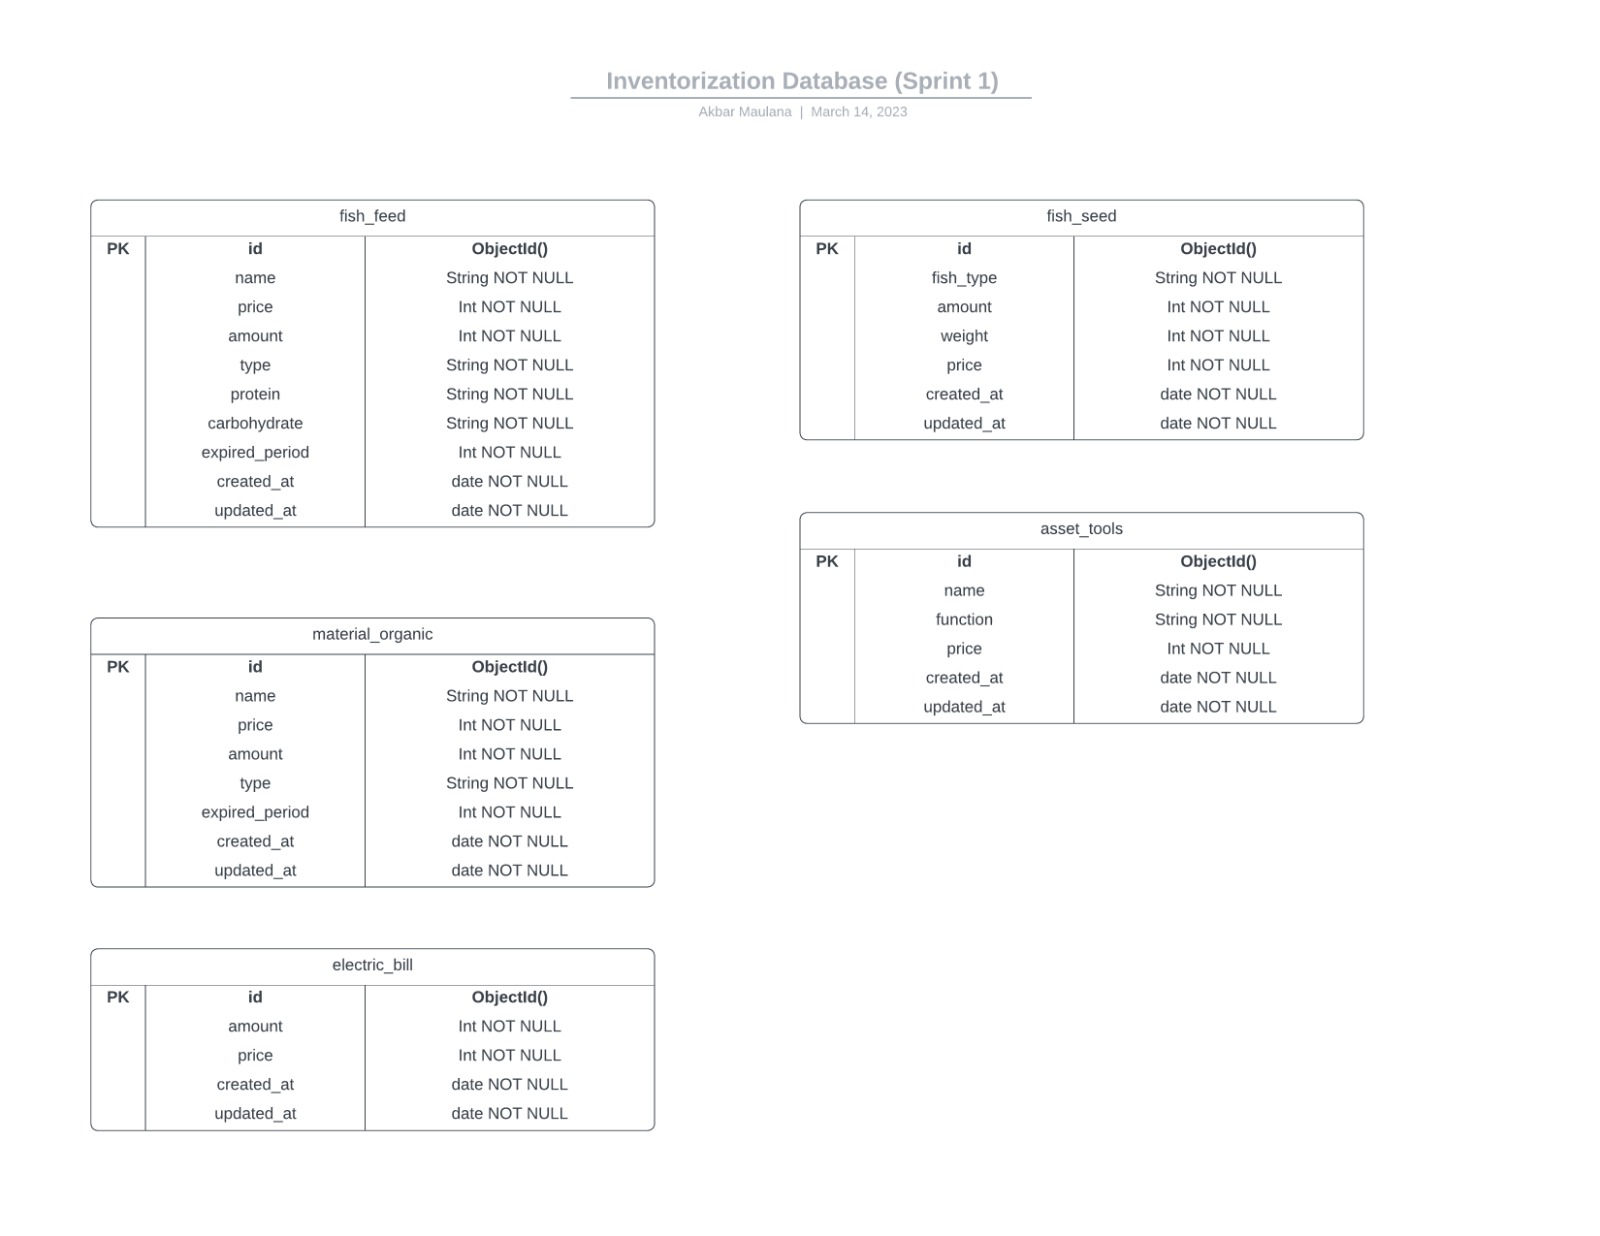
\includegraphics[width=1\textwidth]{gambar/sprint1/sprint1_inventaris_database.jpeg}
		\caption{Skema Database Fitur Inventaris}
	\end{figure}

	Dari skema database tersebut, terdapat lima opsi kategori inventaris yang sudah dijelaskan sebelumnya. Pada skema database ini, masing-masing kategori memiliki kebutuhan yang berbeda antara lain.

	\begin{enumerate}
		\item fish\_feed (Pakan Ikan)
		\item material\_organic (Bahan Organik)
		\item electric\_bill (Tagihan Listrik)
		\item fish\_seed (Benih Ikan)
		\item asset\_tools (Peralatan)
	\end{enumerate}

	Dalam tabel database tersebut, pada kolom pertama terdapat jenis \textit{key} yang dijadikan patokan dalam tabel database tersebut. Kemudian kolom kedua dan ketiga merupakan hubungan antara nama data dan tipe data yang mewakili nama data tersebut.

	Setelah skema database dari inventaris telah dibuat, tabel-tabel database tersebut harus diintegrasikan dengan skema database sebelumnya untuk menyesuaikan kebutuhan fitur yang akan dibuat nantinya. Berikut merupakan skema database yang telah diintegrasikan dengan skema database dari inventaris dapat dilihat pada \textbf{Gambar 4.2}.

	\begin{figure}[H]
		\centering
		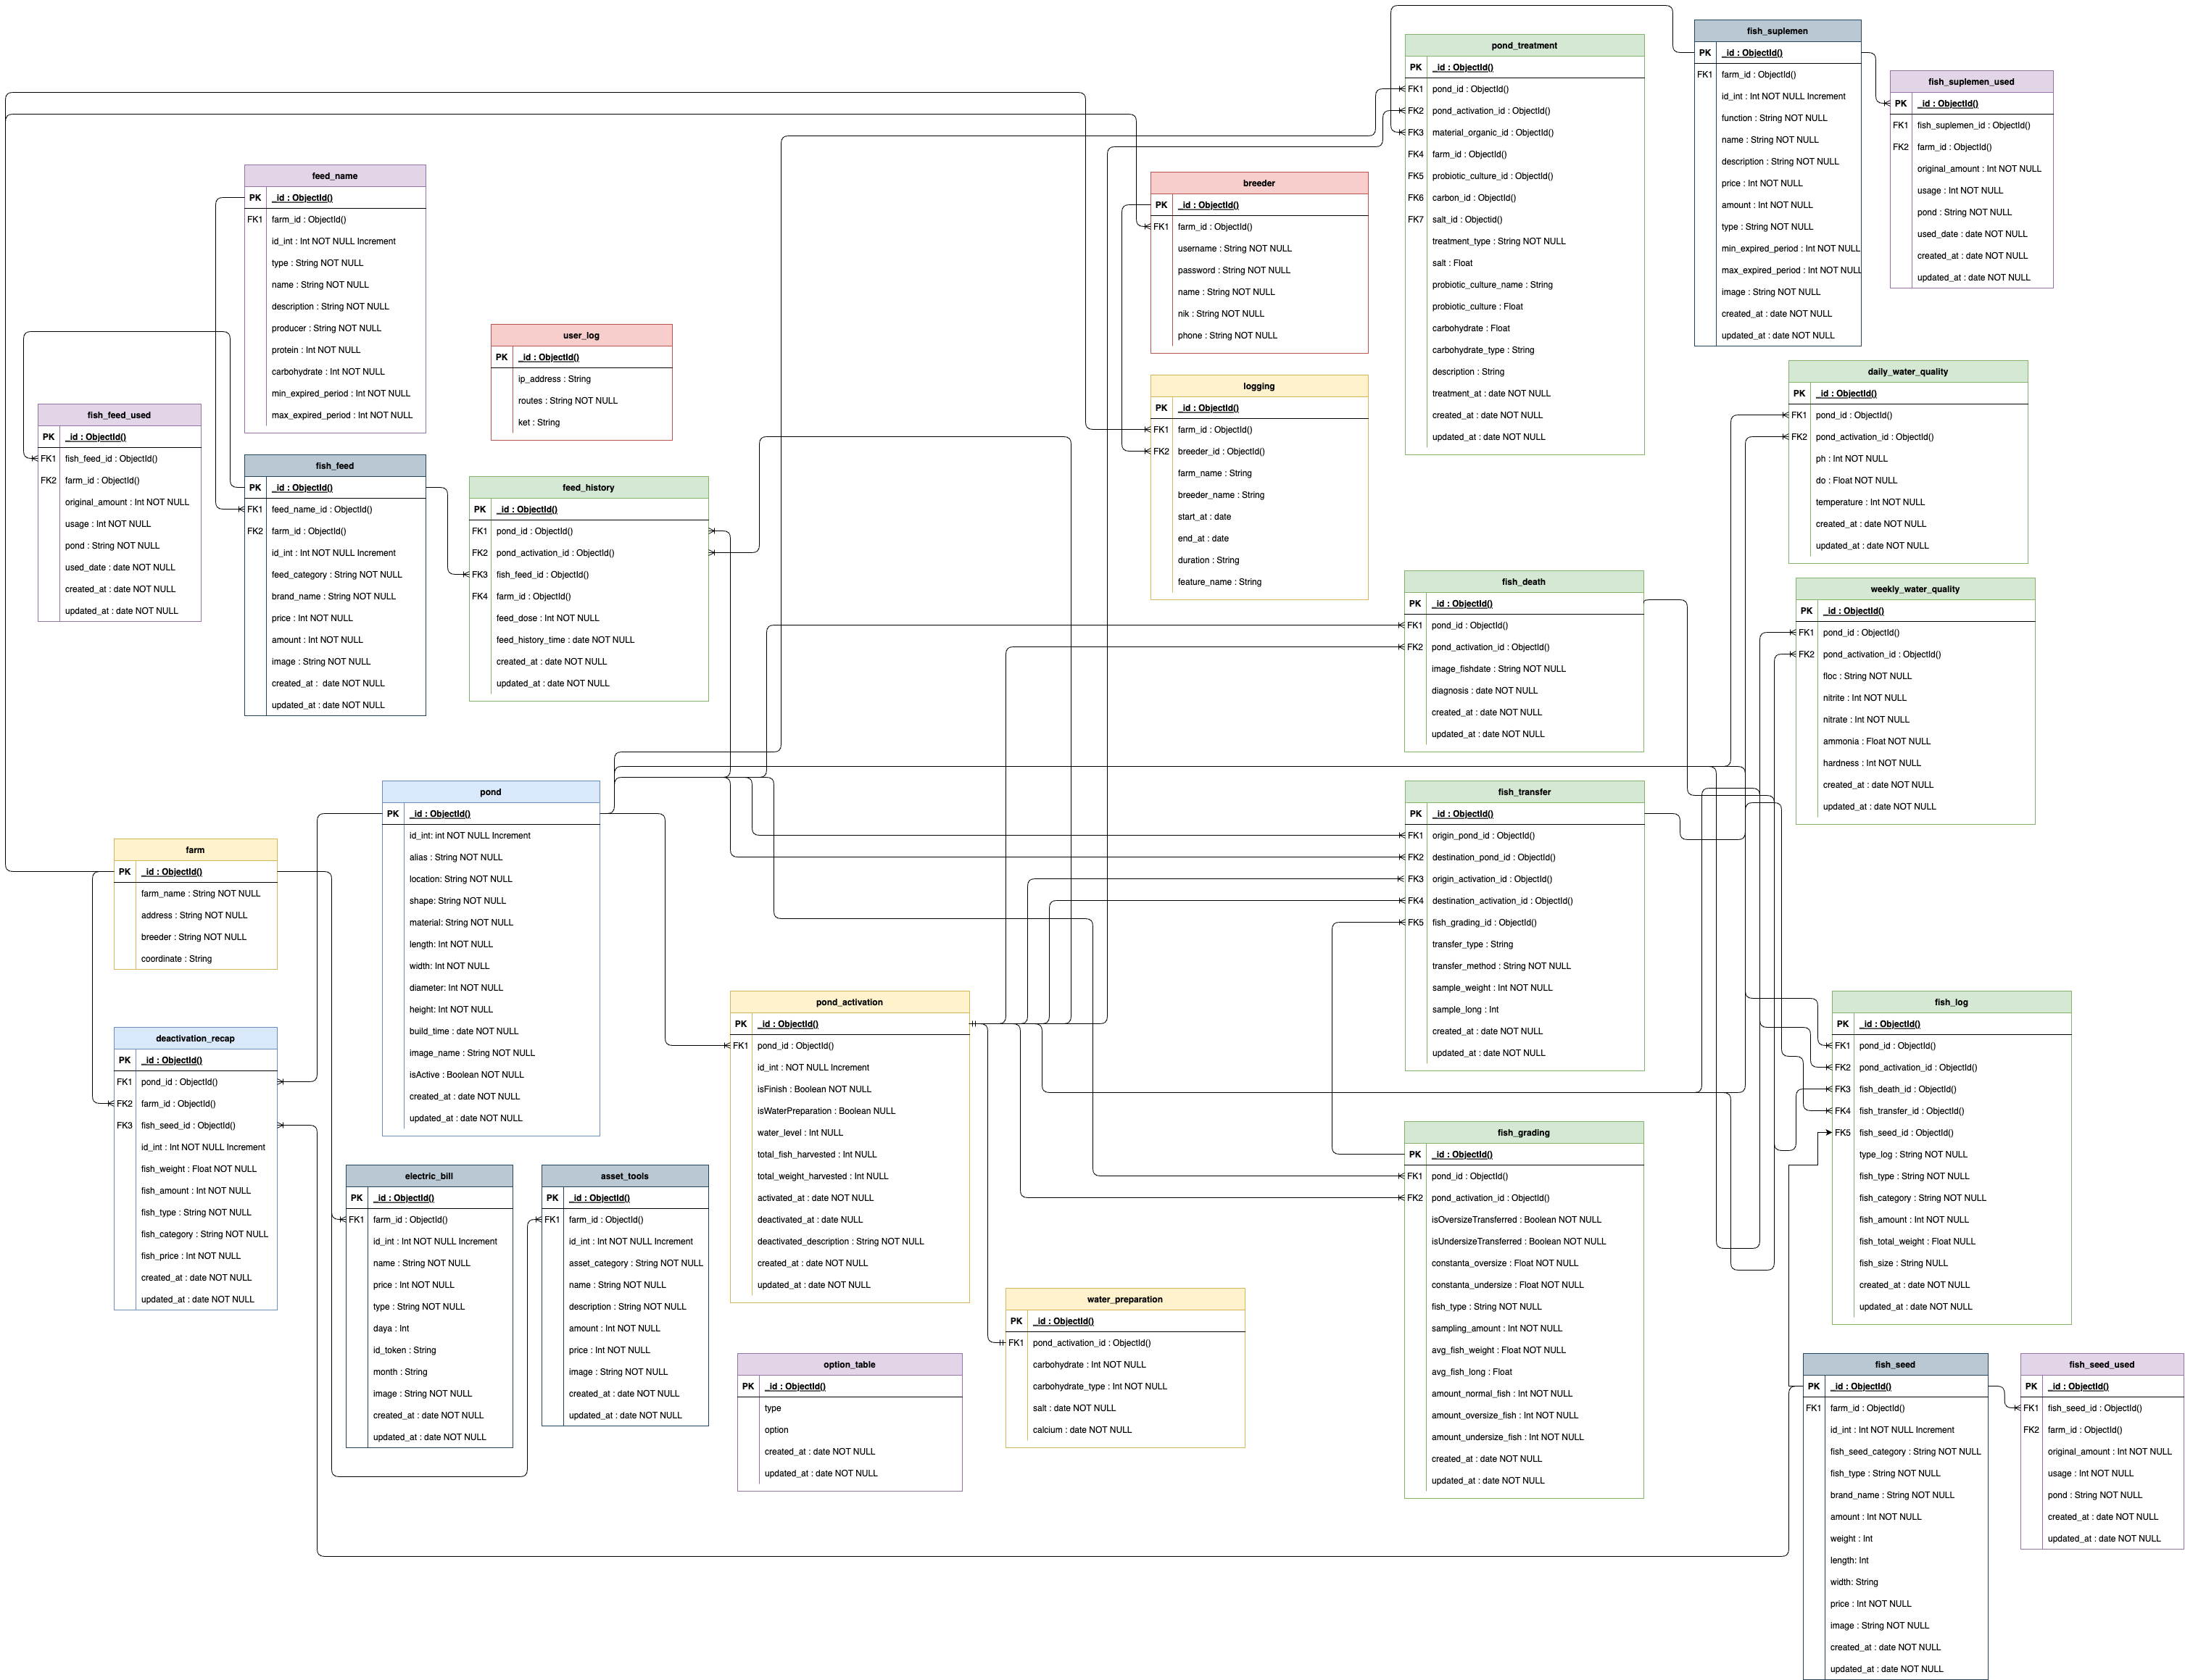
\includegraphics[width=1.5\linewidth,height=1.00\linewidth, angle=270]{gambar/sprint1/sprint1_skema_database.png}
		\caption{Integrasi Database Inventaris dengan Skema Database Iterasi 1}
	\end{figure}

	Dari integrasi diatas, tabel fish\_feed diintegrasikan dengan tabel feed\_type yang digunakan untuk input pakan dan tabel material\_organic diintegrasikan dengan tabel pond\_treatment karena dalam fitur treatment kolam diperlukan data dari tabel material organik tersebut. Lalu tabel fish\_seed diintegrasikan dengan tabel pond\_activation dan fish\_log untuk aktivasi kolam dan perhitungan jumlah ikan. Sementara itu, tabel electric\_bill dan asset\_tools merupakan individu yang tidak terintegrasi dengan tabel yang lain. Hal ini dikarenakan tabel tersebut hanya untuk menyimpan datanya saja dan tidak digunakan di dalam fitur.
	
	Berikut merupakan mockup dari fitur inventaris yang mencakup skema database sebelumnya.

	\begin{figure}[H]
		\hspace{.15\linewidth}
		\minipage{0.32\textwidth}
			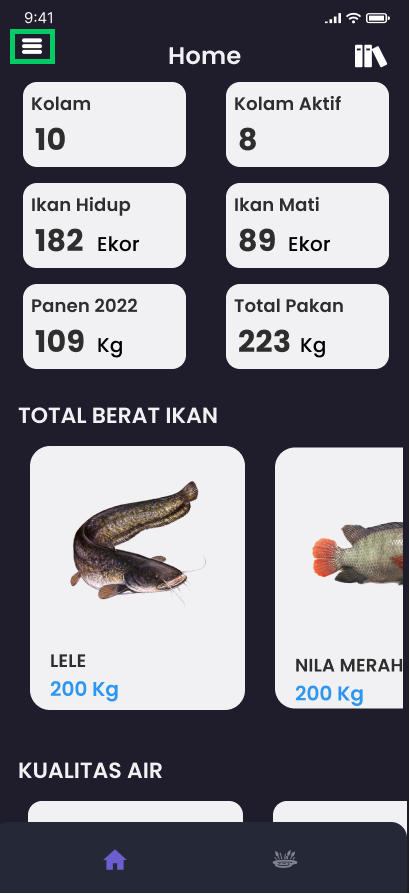
\includegraphics[width=\linewidth]{gambar/sprint1/mockup_dashboard.png}
			\caption{Halaman Dashboard}
		\endminipage\hfill
		\minipage{0.32\textwidth}
			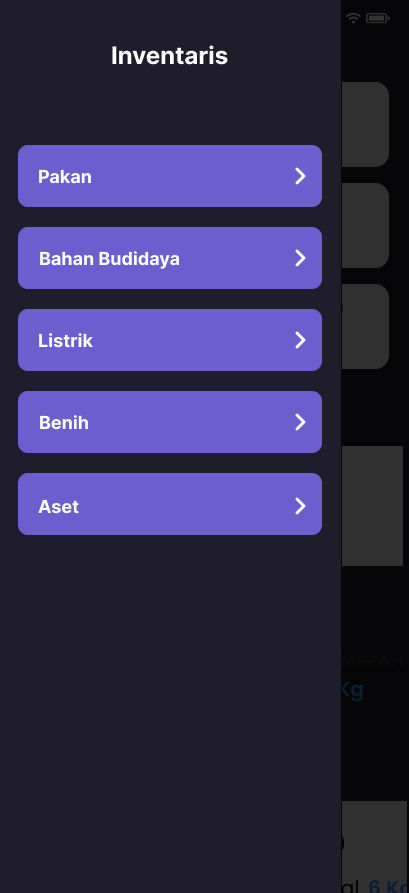
\includegraphics[width=\linewidth]{gambar/sprint1/mockup_home.png}
			\caption{Halaman Menu Inventaris}
		\endminipage
		\hspace{.05\linewidth}
	\end{figure}

	Pada halaman dashboard, dipojok kiri atas terdapat ikon \textit{hamburger} atau list yang ketika ditekan akan menampilkan halaman menu inventaris seperti \textbf{Gambar 4.4}. Masing-masing list menu yang ada pada halaman menu inventaris memiliki fungsi yang sesuai dengan skema inventaris.

	\begin{figure}[H]
		\minipage{0.32\textwidth}
			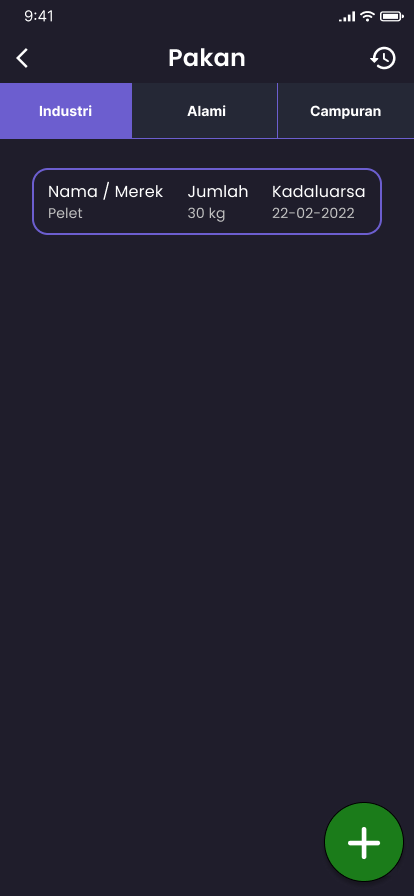
\includegraphics[width=\linewidth]{gambar/sprint1/mockup_detail_feed.png}
			\caption{Halaman Data Inventaris Pakan}
		\endminipage\hfill
		\minipage{0.32\textwidth}
			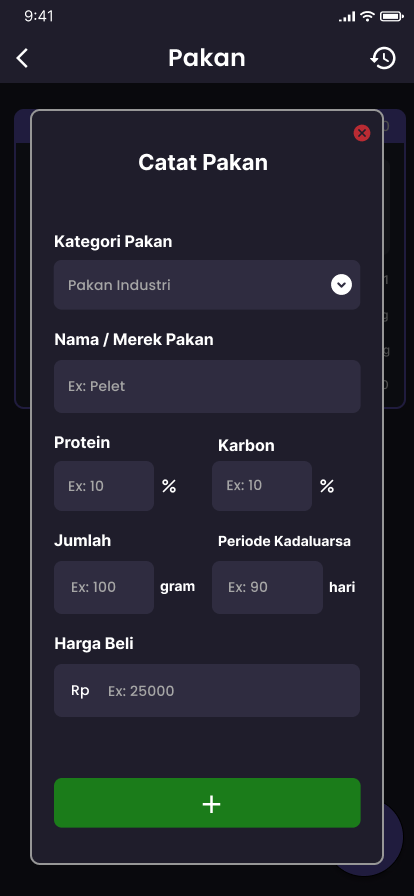
\includegraphics[width=\linewidth]{gambar/sprint1/mockup_input_feed.png}
			\caption{Halaman Input Inventaris Pakan}
		\endminipage\hfill
		\minipage{0.32\textwidth}%
			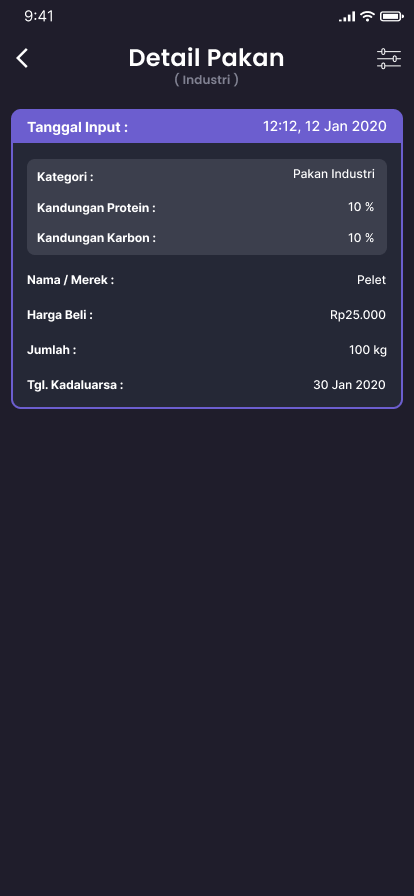
\includegraphics[width=\linewidth]{gambar/sprint1/mockup_list_feed.png}
			\caption{Halaman Detail Inventaris Pakan}
		\endminipage
	\end{figure}

	Jika pada halaman menu inventaris sebelumnya dipilih menu "Pakan", maka akan masuk ke halaman data inventaris pakan. Pada halaman ini terdapat 3 jenis pakan yaitu pakan industri (pelet), alami (tumbuh-tumbuhan), serta campuran (tepung, terigu, dll). Masing-masing jenis pakan memiliki detail data yaitu nama atau merek pakan, total jumlah pakan yang tersedia, serta tanggal kadaluarsa dari pakan tersebut.

	Tombol (+) yang ada di pojok kanan bawah akan mengarahkan ke halaman input dari inventaris pakan. Disini diberikan form input yang beragam seperti yang ada pada \textbf{Gambar 4.6}.

	Sementara tombol riwayat yang ada di pojok kanan atas akan mengarahkan ke halaman detail dari inventaris pakan. Di halaman ini ditampilkan detail pemasukkan pakan ke sistem inventaris.

	\begin{figure}[H]
		\minipage{0.32\textwidth}
			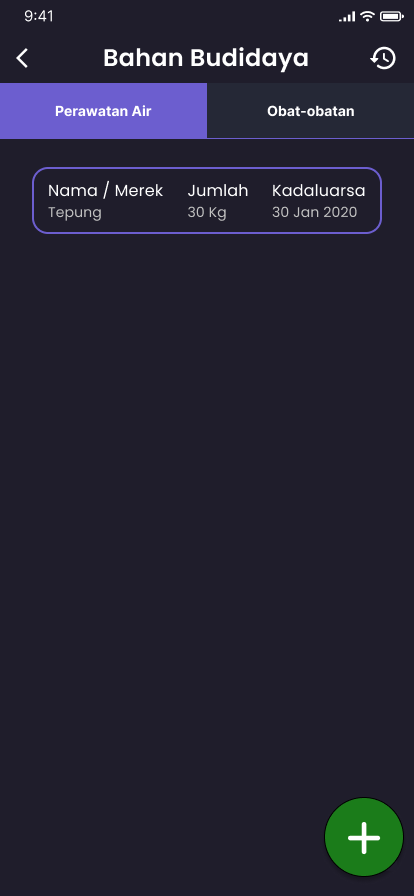
\includegraphics[width=\linewidth]{gambar/sprint1/mockup_detail_materials.png}
			\caption{Halaman Data Inventaris Bahan Budidaya}
		\endminipage\hfill
		\minipage{0.32\textwidth}
			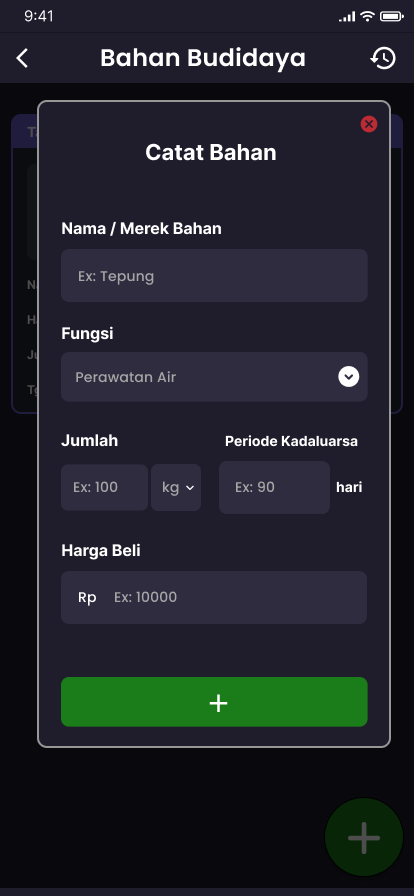
\includegraphics[width=\linewidth]{gambar/sprint1/mockup_input_materials.png}
			\caption{Halaman Input Inventaris Bahan Budidaya}
		\endminipage\hfill
		\minipage{0.32\textwidth}%
			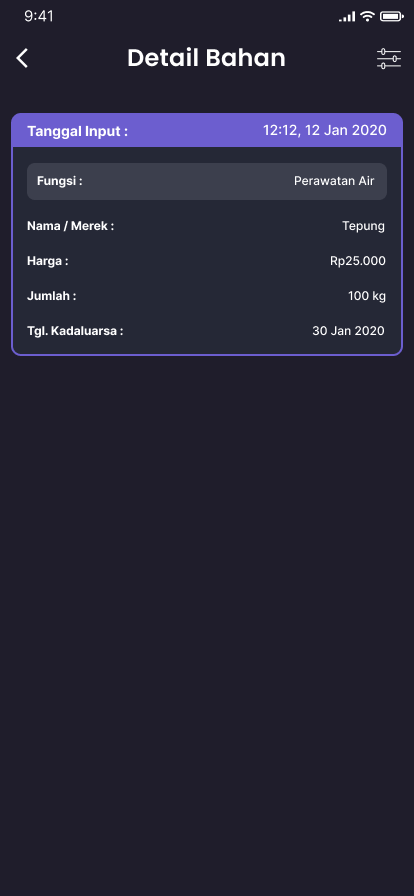
\includegraphics[width=\linewidth]{gambar/sprint1/mockup_list_materials.png}
			\caption{Halaman Detail Inventaris Bahan Budidaya}
		\endminipage
	\end{figure}

	Jika pada halaman menu inventaris sebelumnya dipilih menu "Bahan Budidaya", maka akan masuk ke halaman data inventaris bahan budidaya. Pada halaman ini terdapat 2 jenis bahan budidaya yang dibagi berdasarkan fungsi yaitu perawatan air dan obat-obatan (Methylene Blue, dll). Sama seperti pada inventaris pakan, masing-masing jenis bahan budidaya memiliki detail data yaitu nama atau merek, total jumlah yang tersedia, serta tanggal kadaluarsa.

	Sama seperti halaman inventaris pakan, tombol (+) mengarahkan ke halaman input seperti \textbf{Gambar 4.9} dan tombol riwayat akan mengarahkan ke halaman detail inventaris seperti pada \textbf{Gambar 4.10}.

	\begin{figure}[H]
		\minipage{0.32\textwidth}
			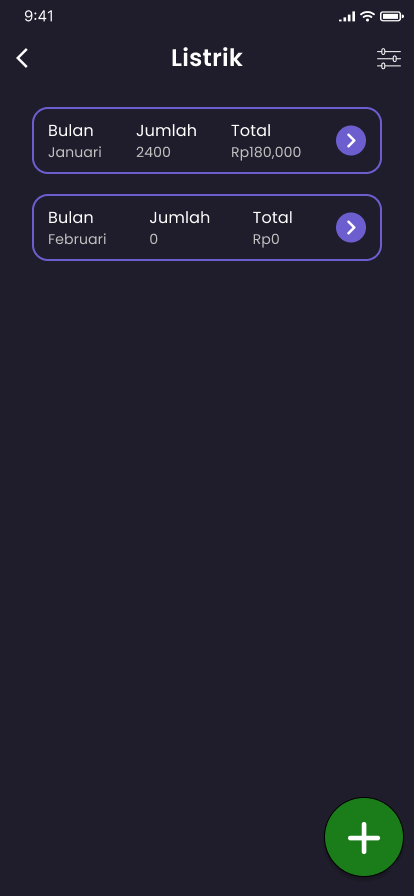
\includegraphics[width=\linewidth]{gambar/sprint1/mockup_detail_electric.png}
			\caption{Halaman Data Inventaris Tagihan Listrik}
		\endminipage\hfill
		\minipage{0.32\textwidth}
			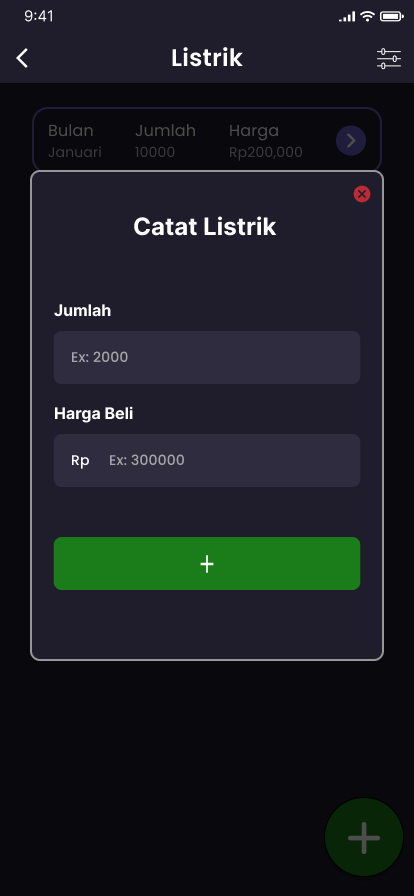
\includegraphics[width=\linewidth]{gambar/sprint1/mockup_input_electric.png}
			\caption{Halaman Input Inventaris Tagihan Listrik}
		\endminipage\hfill
		\minipage{0.32\textwidth}%
			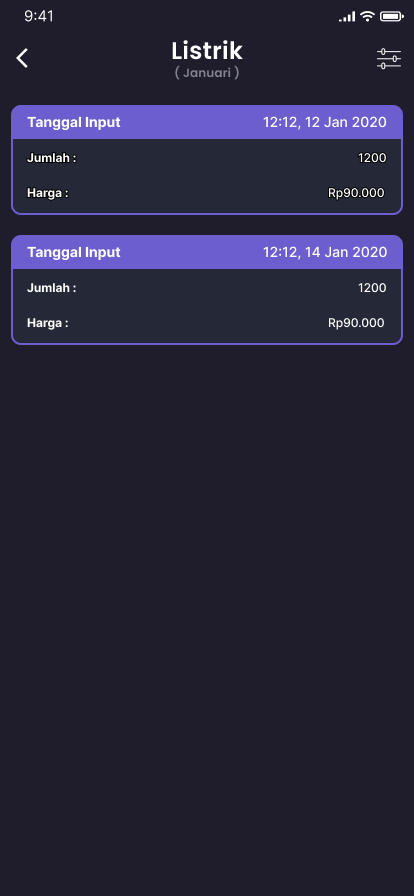
\includegraphics[width=\linewidth]{gambar/sprint1/mockup_list_electric.png}
			\caption{Halaman Detail Inventaris Tagihan Listrik}
		\endminipage
	\end{figure}

	Jika pada halaman menu inventaris sebelumnya dipilih menu "Listrik", maka akan masuk ke halaman data inventaris tagihan listrik. Pada halaman ini terdapat list dari tagihan listrik perbulannya yang digunakan oleh pembudidaya, data yang ditampilkan berupa bulan, jumlah listrik, serta total biaya tagihan. Jika list bulan tersebut ditekan, maka akan pindah ke halaman detail dari tagihan listrik dibulan tersebut. 

	Untuk tombol (+) yang ada di pojok kanan bawah, jika ditekan akan masuk ke halaman input tagihan. Form yang harus diisi hanya jumlah token listrik dan harga belinya. Sementara tombol filter yang ada di pojok kanan atas berfungsi untuk memfilter data sesuai keinginan user.

	\begin{figure}[H]
		\minipage{0.32\textwidth}
			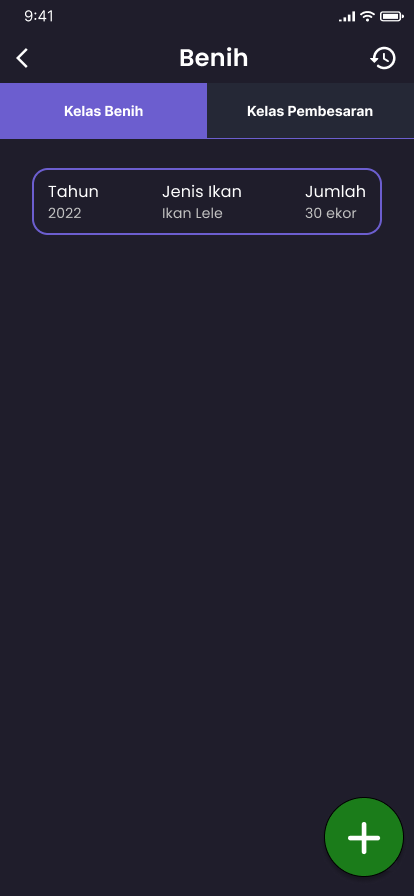
\includegraphics[width=\linewidth]{gambar/sprint1/mockup_detail_seed.png}
			\caption{Halaman Data Inventaris Benih}
		\endminipage\hfill
		\minipage{0.32\textwidth}
			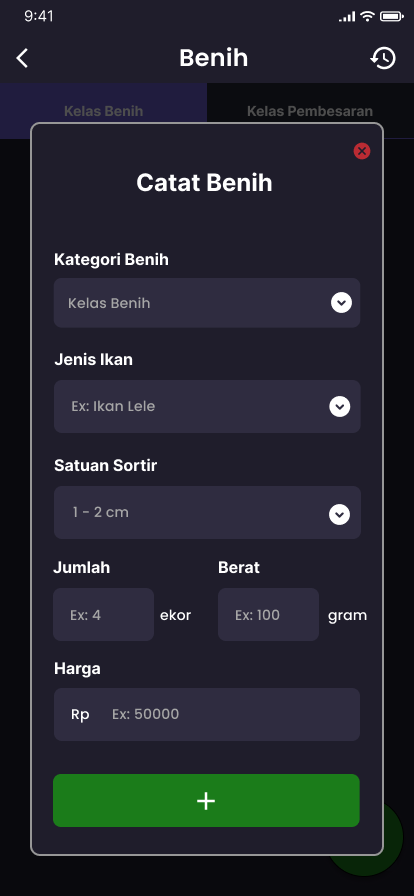
\includegraphics[width=\linewidth]{gambar/sprint1/mockup_input_seed.png}
			\caption{Halaman Input Inventaris Benih}
		\endminipage\hfill
		\minipage{0.32\textwidth}%
			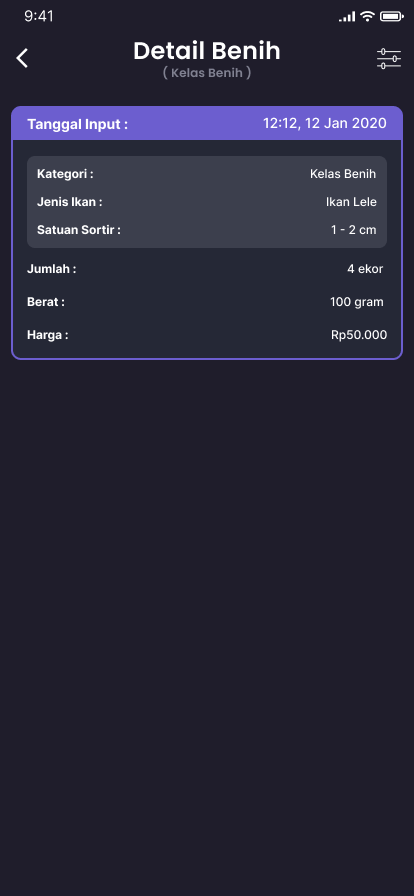
\includegraphics[width=\linewidth]{gambar/sprint1/mockup_list_seed.png}
			\caption{Halaman Detail Inventaris Benih}
		\endminipage
	\end{figure}

	Jika pada halaman menu inventaris sebelumnya dipilih menu "Benih", maka akan masuk ke halaman data inventaris benih. Pada halaman ini terdapat list dari benih yang sudah diinput pada sistem inventaris yang terbagi menjadi dua jenis yaitu benih jenis kelas benih (kecil) dan kelas pembesaran (besar). Masing-masing data memiliki detail seperti tahun benih di input, jenis benih, dan jumlah dari benih.

	Untuk tombol (+) yang ada di pojok kanan bawah, jika ditekan akan dinavigasikan ke halaman input benih ikan. Halaman input ini memiliki form seperti pada \textbf{Gambar 4.15}. Terdapat dua jenis form yang berbeda berdasarkan ketegori yang dipilih, untuk kategori kelas benih pada bagian ukurannya menggunakan satuan sortir sementara untuk kategori kelas pembesaran menggunakan panjang dan lebar untuk ukurannya.

	\begin{figure}[H]
		\hspace{.15\linewidth}
		\minipage{0.32\textwidth}
			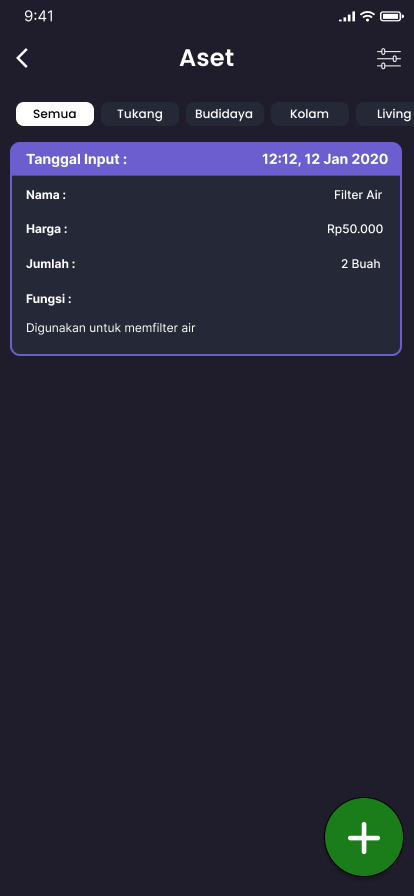
\includegraphics[width=\linewidth]{gambar/sprint1/mockup_list_aset.png}
			\caption{Halaman Data Inventaris Aset}
		\endminipage\hfill
		\minipage{0.32\textwidth}%
			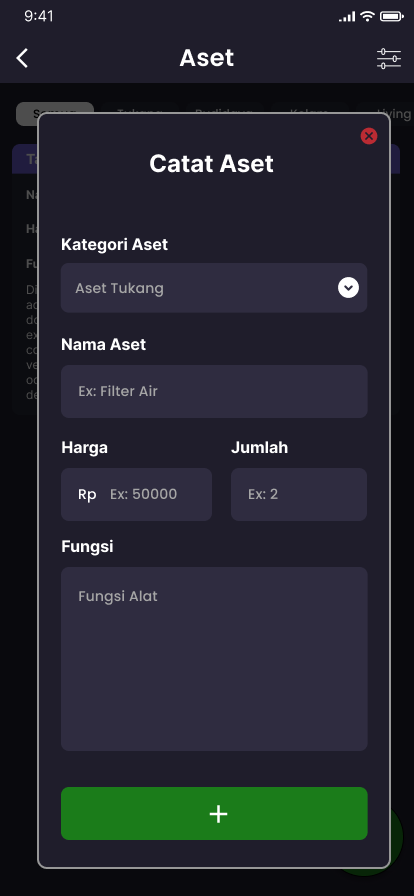
\includegraphics[width=\linewidth]{gambar/sprint1/mockup_input_aset.png}
			\caption{Halaman Input Inventaris Aset}
		\endminipage
		\hspace{.05\linewidth}
	\end{figure}

	Jika pada halaman menu inventaris sebelumnya dipilih menu "Aset", maka akan masuk ke halaman data inventaris aset. Pada halaman ini, ditampilkan jenis dari aset-aset yang digunakan selama masa budidaya.
	
	Aset dibagi menjadi empat jenis kategori yaitu aset tukang (aset yang diperlukan pembudidaya), aset budidaya (aset yang dibutuhkan selama budidaya berlangsung), aset kolam (aset yang digunakan dalam kolam budidaya), dan aset living (aset yang diperlukan selama berlangsungnya musim budidaya).

	Tombol (+) pada pojok kanan bawah berfungsi untuk navigasi ke halaman input sementara tombol filter pada pojok kanan atas berfungsi untuk filter data.

\subsection{Sprint 2}


Sprint 2 dilaksanakan pada tanggal 30 Maret 2023 - 15 April 2023. Detail dari Sprint 2 ini adalah mengerjakan tugas yang ada pada Sprint 2 Backlog di tabel berikut.
		
	\begin{table}[H]	
		\begin{center}
			\caption{Sprint 2 Backlog}
			\label{tab:table7}
			\begin{tabular}{|c|c|m{13em}|c|}
			\hline
			\textbf{No} & \textbf{Stories} & \textbf{Task} & \textbf{Status} \\
			\hline
			1 & \multirow{2}{12em}{Fitur pencatatan inventaris} & - Membuat alur UI/UX dari design aplikasi & Selesai \\
			&  & - Mengupdate skema database pada inventaris & Selesai \\ 
			% &  & -  & Selesai \\ 
			\hline
			\end{tabular}
		\end{center}
	\end{table}

	Selama masa Sprint 2 berlangsung, tim bertemu dengan perwakilan dari Dinas Perikanan Bogor. Dari pertemuan itu, salah satunya terdapat beberapa perubahan user requirement sehingga perlu merubah skema database yang sudah dibuat pada Sprint 1. Lalu, terdapat juga pertimbangan perubahan penentuan harga jual ikan dengan ditambahkannya perhitungan aset namun hal ini belum ditentukan akan masuk perhitungan atau tidak. 

	Berikut merupakan alur user sebagai pengguna aplikasi berdasarkan mockup yang sudah dibuat pada Sprint 1.

	\begin{figure}[H]
		\centering
		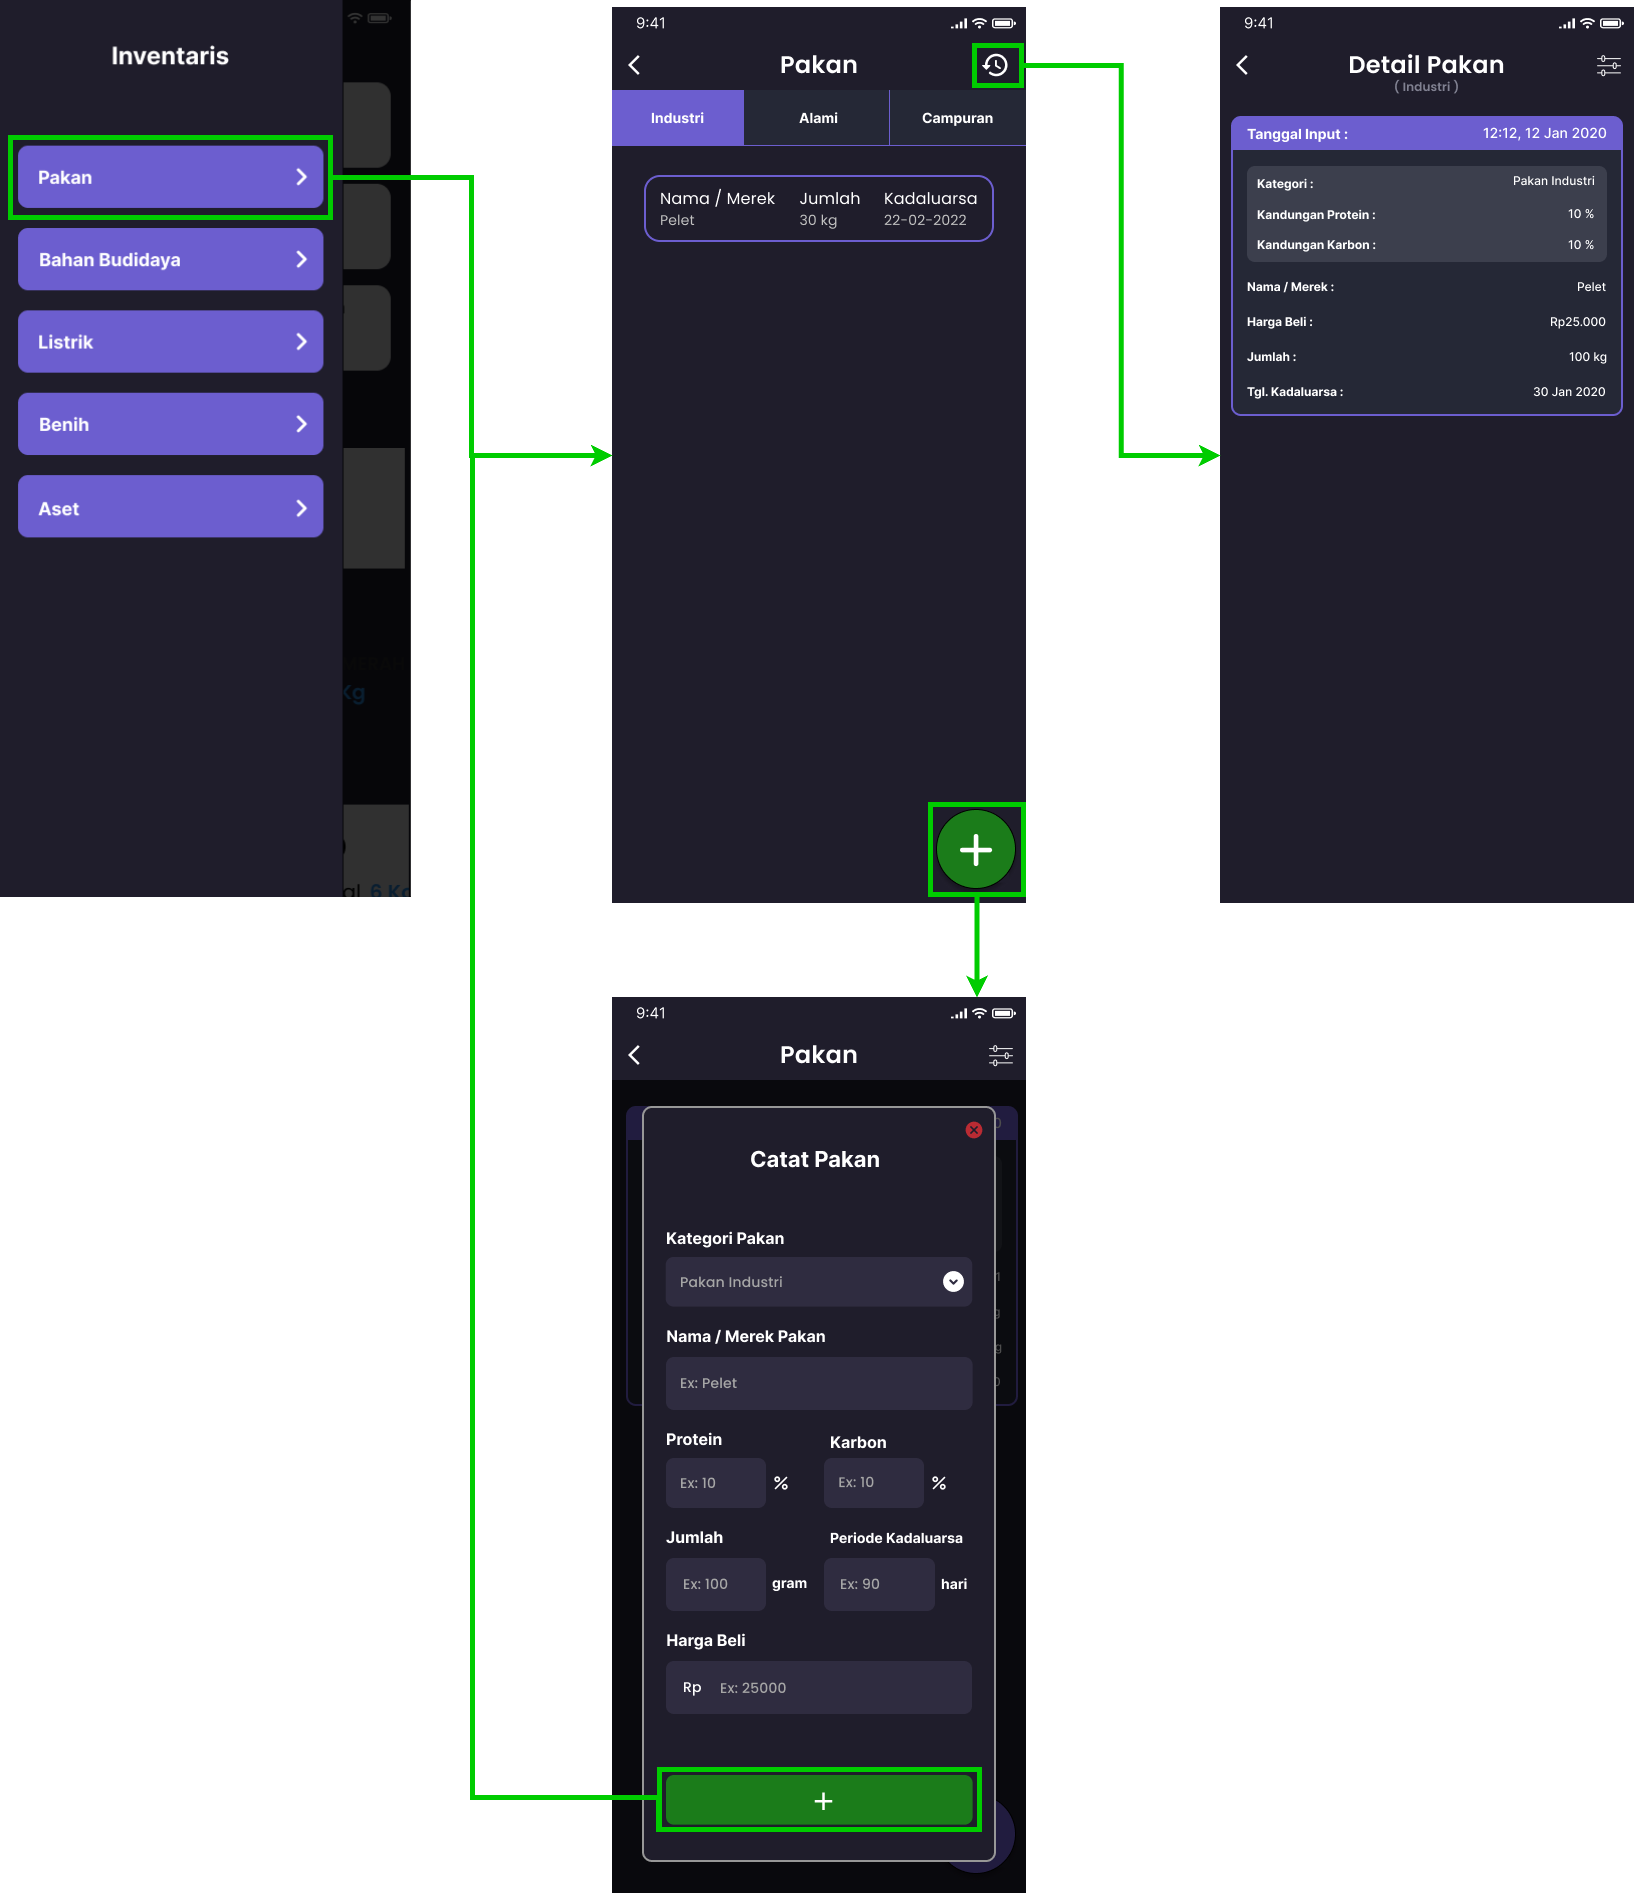
\includegraphics[width=0.9\textwidth]{gambar/sprint2/flow_feed.png}
		\caption{Alur Inventaris Pakan}
	\end{figure}

	Pada \textbf{Gambar 4.19} merupakan alur dari inventaris pakan. Pengguna akan memilih menu "Pakan" dan masuk ke halaman data inventaris pakan, kemudian tombol (+) akan menavigasikan pengguna ke halaman input pakan dan tombol riwayat akan menavigasikan pengguna ke halaman detail input pakan.

	\begin{figure}[H]
		\centering
		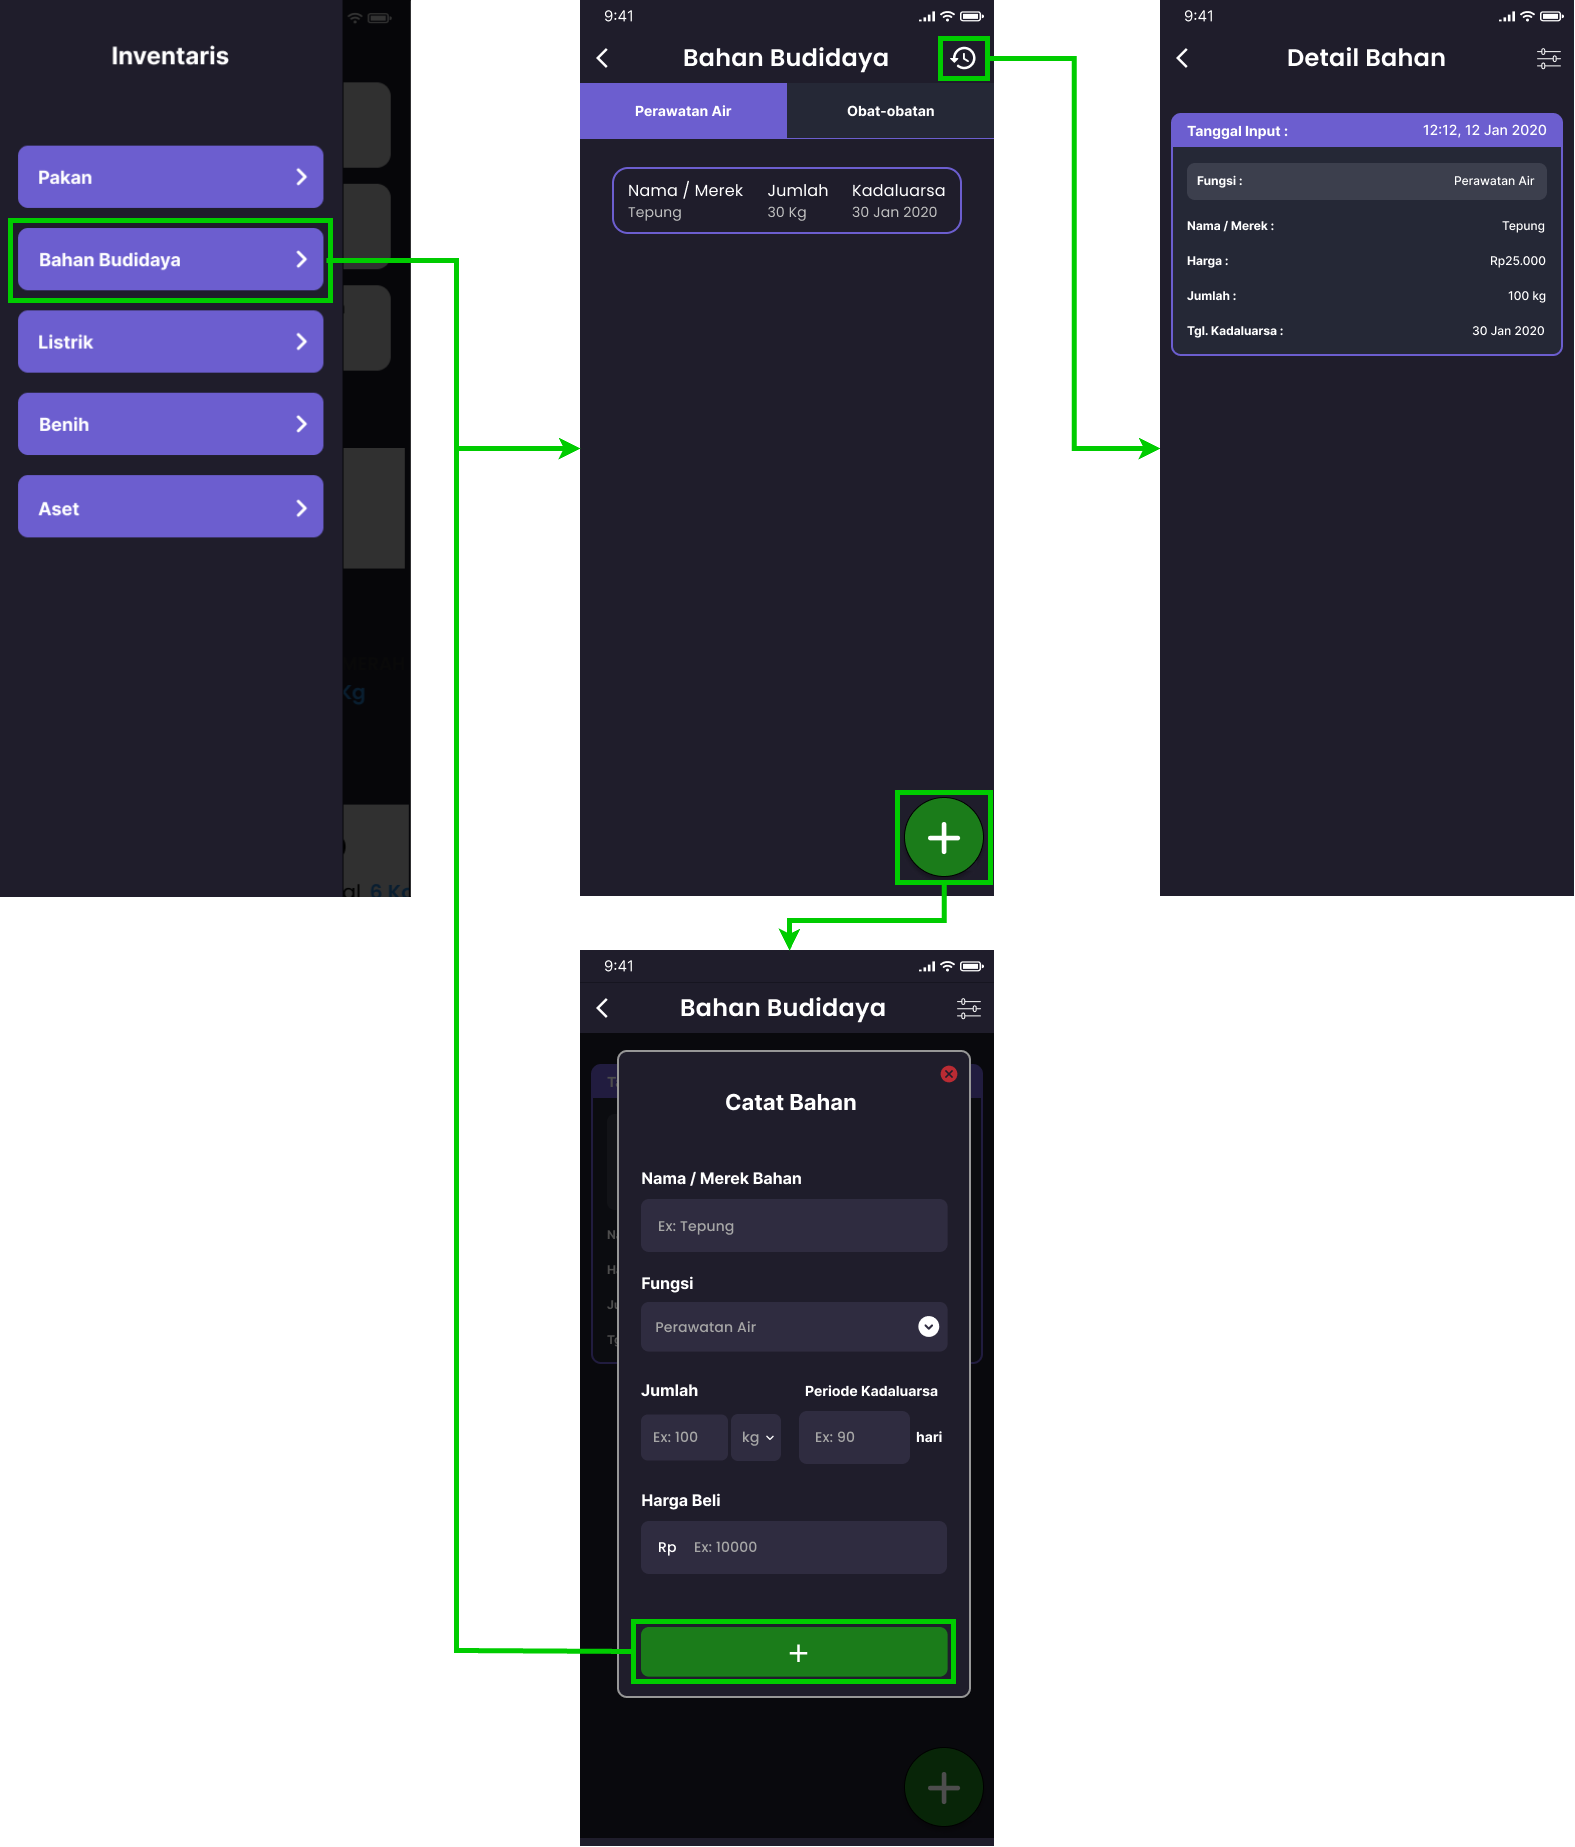
\includegraphics[width=1\textwidth]{gambar/sprint2/flow_materials.png}
		\caption{Alur Inventaris Bahan Budidaya}
	\end{figure}

	Pada \textbf{Gambar 4.20} merupakan alur dari inventaris bahan budidaya. Pengguna akan memilih menu "Bahan Budidaya" dan masuk ke halaman data inventaris budidaya, kemudian tombol (+) akan menavigasikan pengguna ke halaman input bahan budidaya dan tombol riwayat akan menavigasikan pengguna ke halaman detail input bahan budidaya.

	\begin{figure}[H]
		\centering
		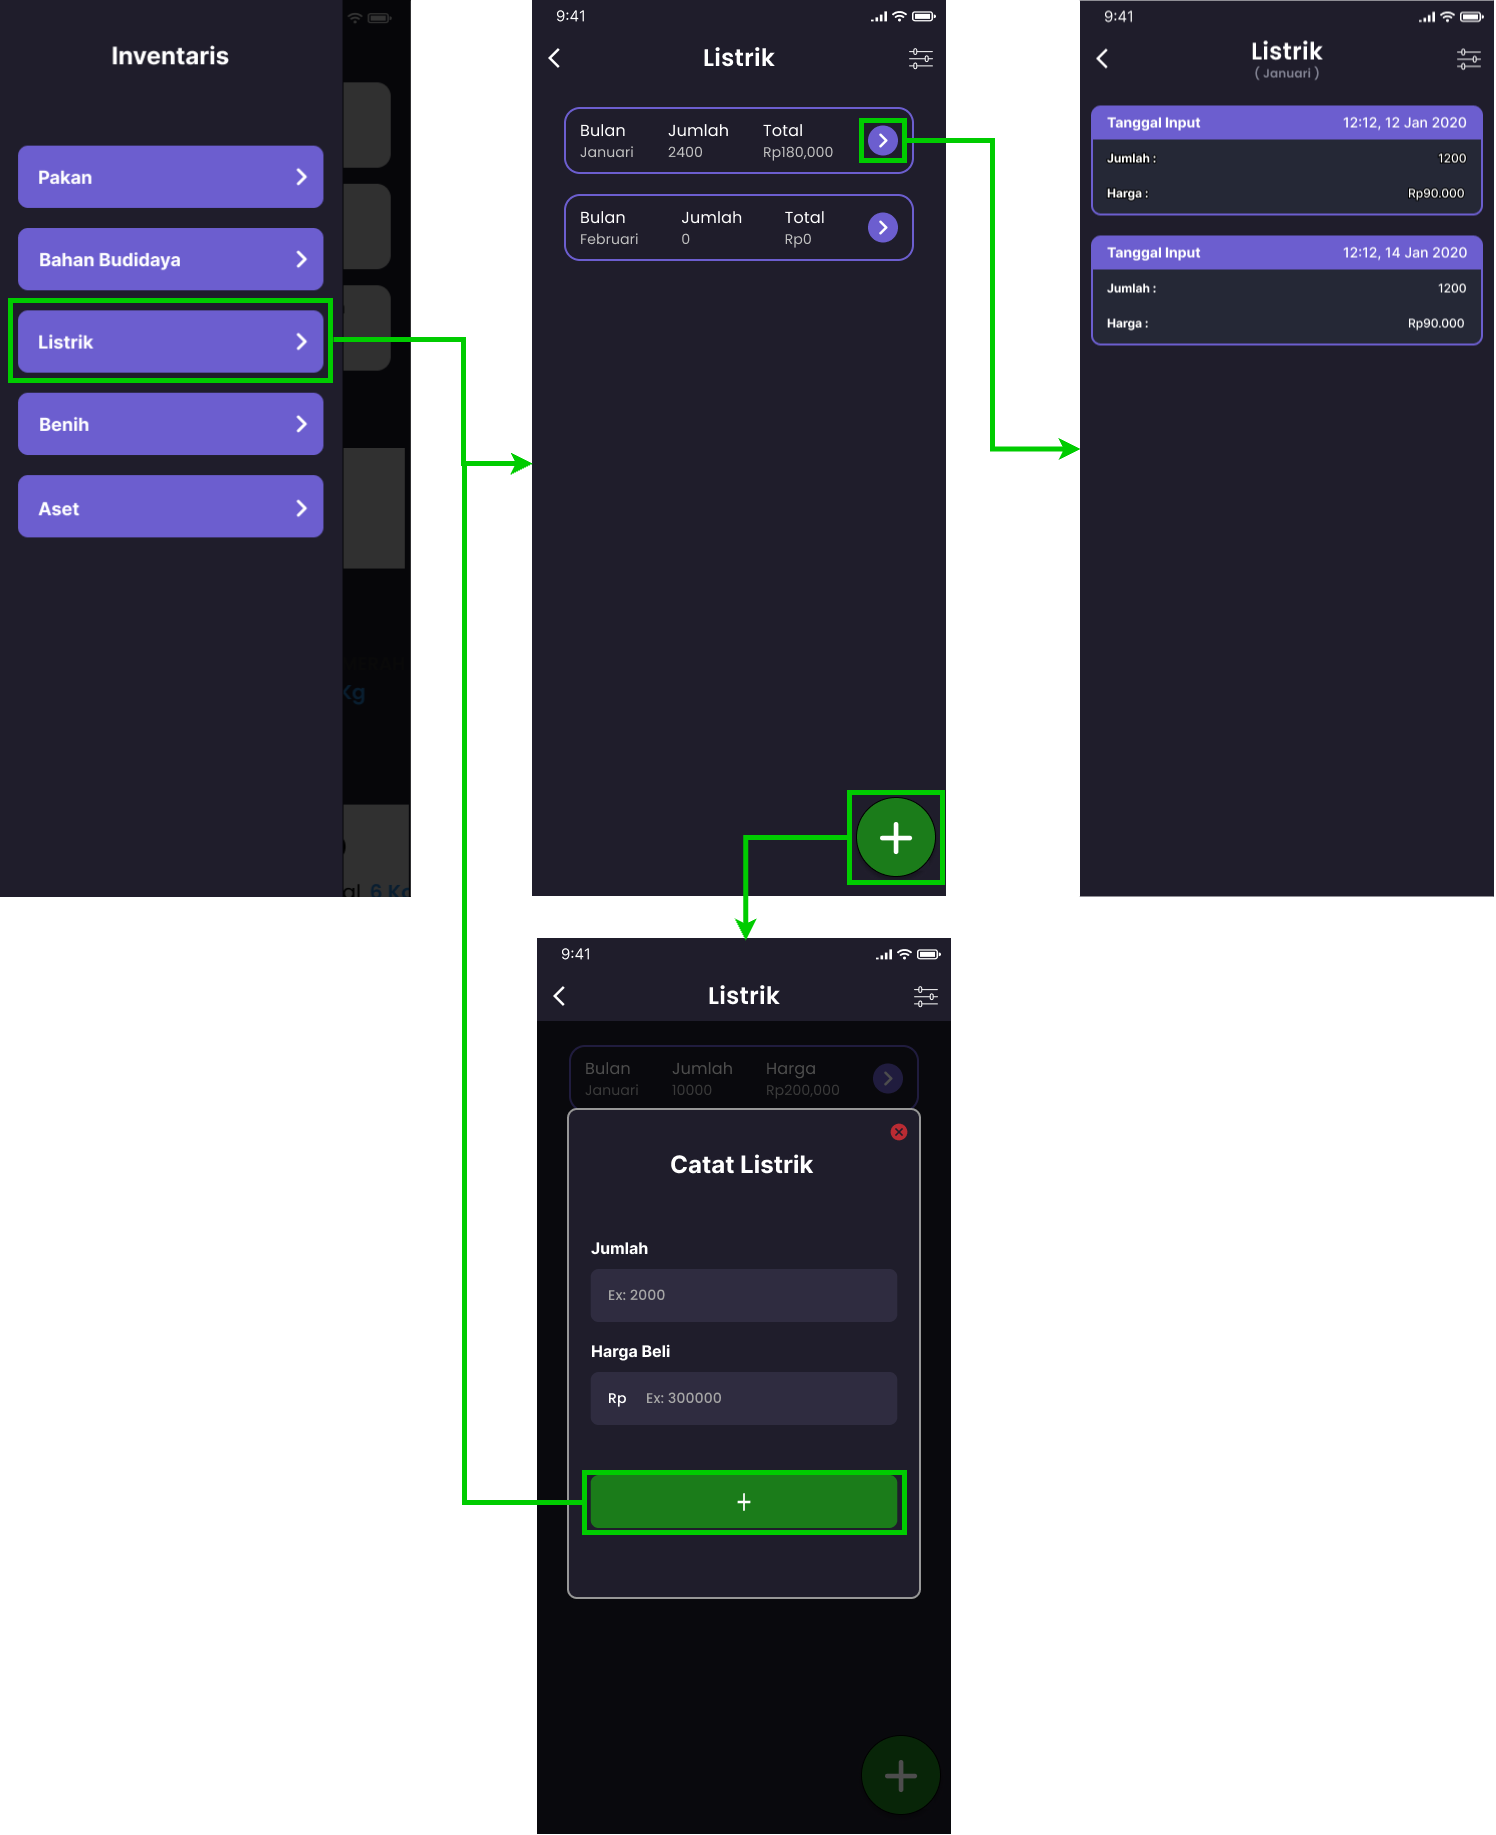
\includegraphics[width=0.9\textwidth]{gambar/sprint2/flow_electric.png}
		\caption{Alur Inventaris Listrik}
	\end{figure}

	Pada \textbf{Gambar 4.21} merupakan alur dari inventaris listrik. Pengguna akan memilih menu "Listrik" dan masuk ke halaman data inventaris listrik, kemudian tombol (+) akan menavigasikan pengguna ke halaman input listrik serta jika pengguna menekan salah satu list bulan pada data listrik, maka akan masuk ke halaman detail input tagihan listrik.

	\begin{figure}[H]
		\centering
		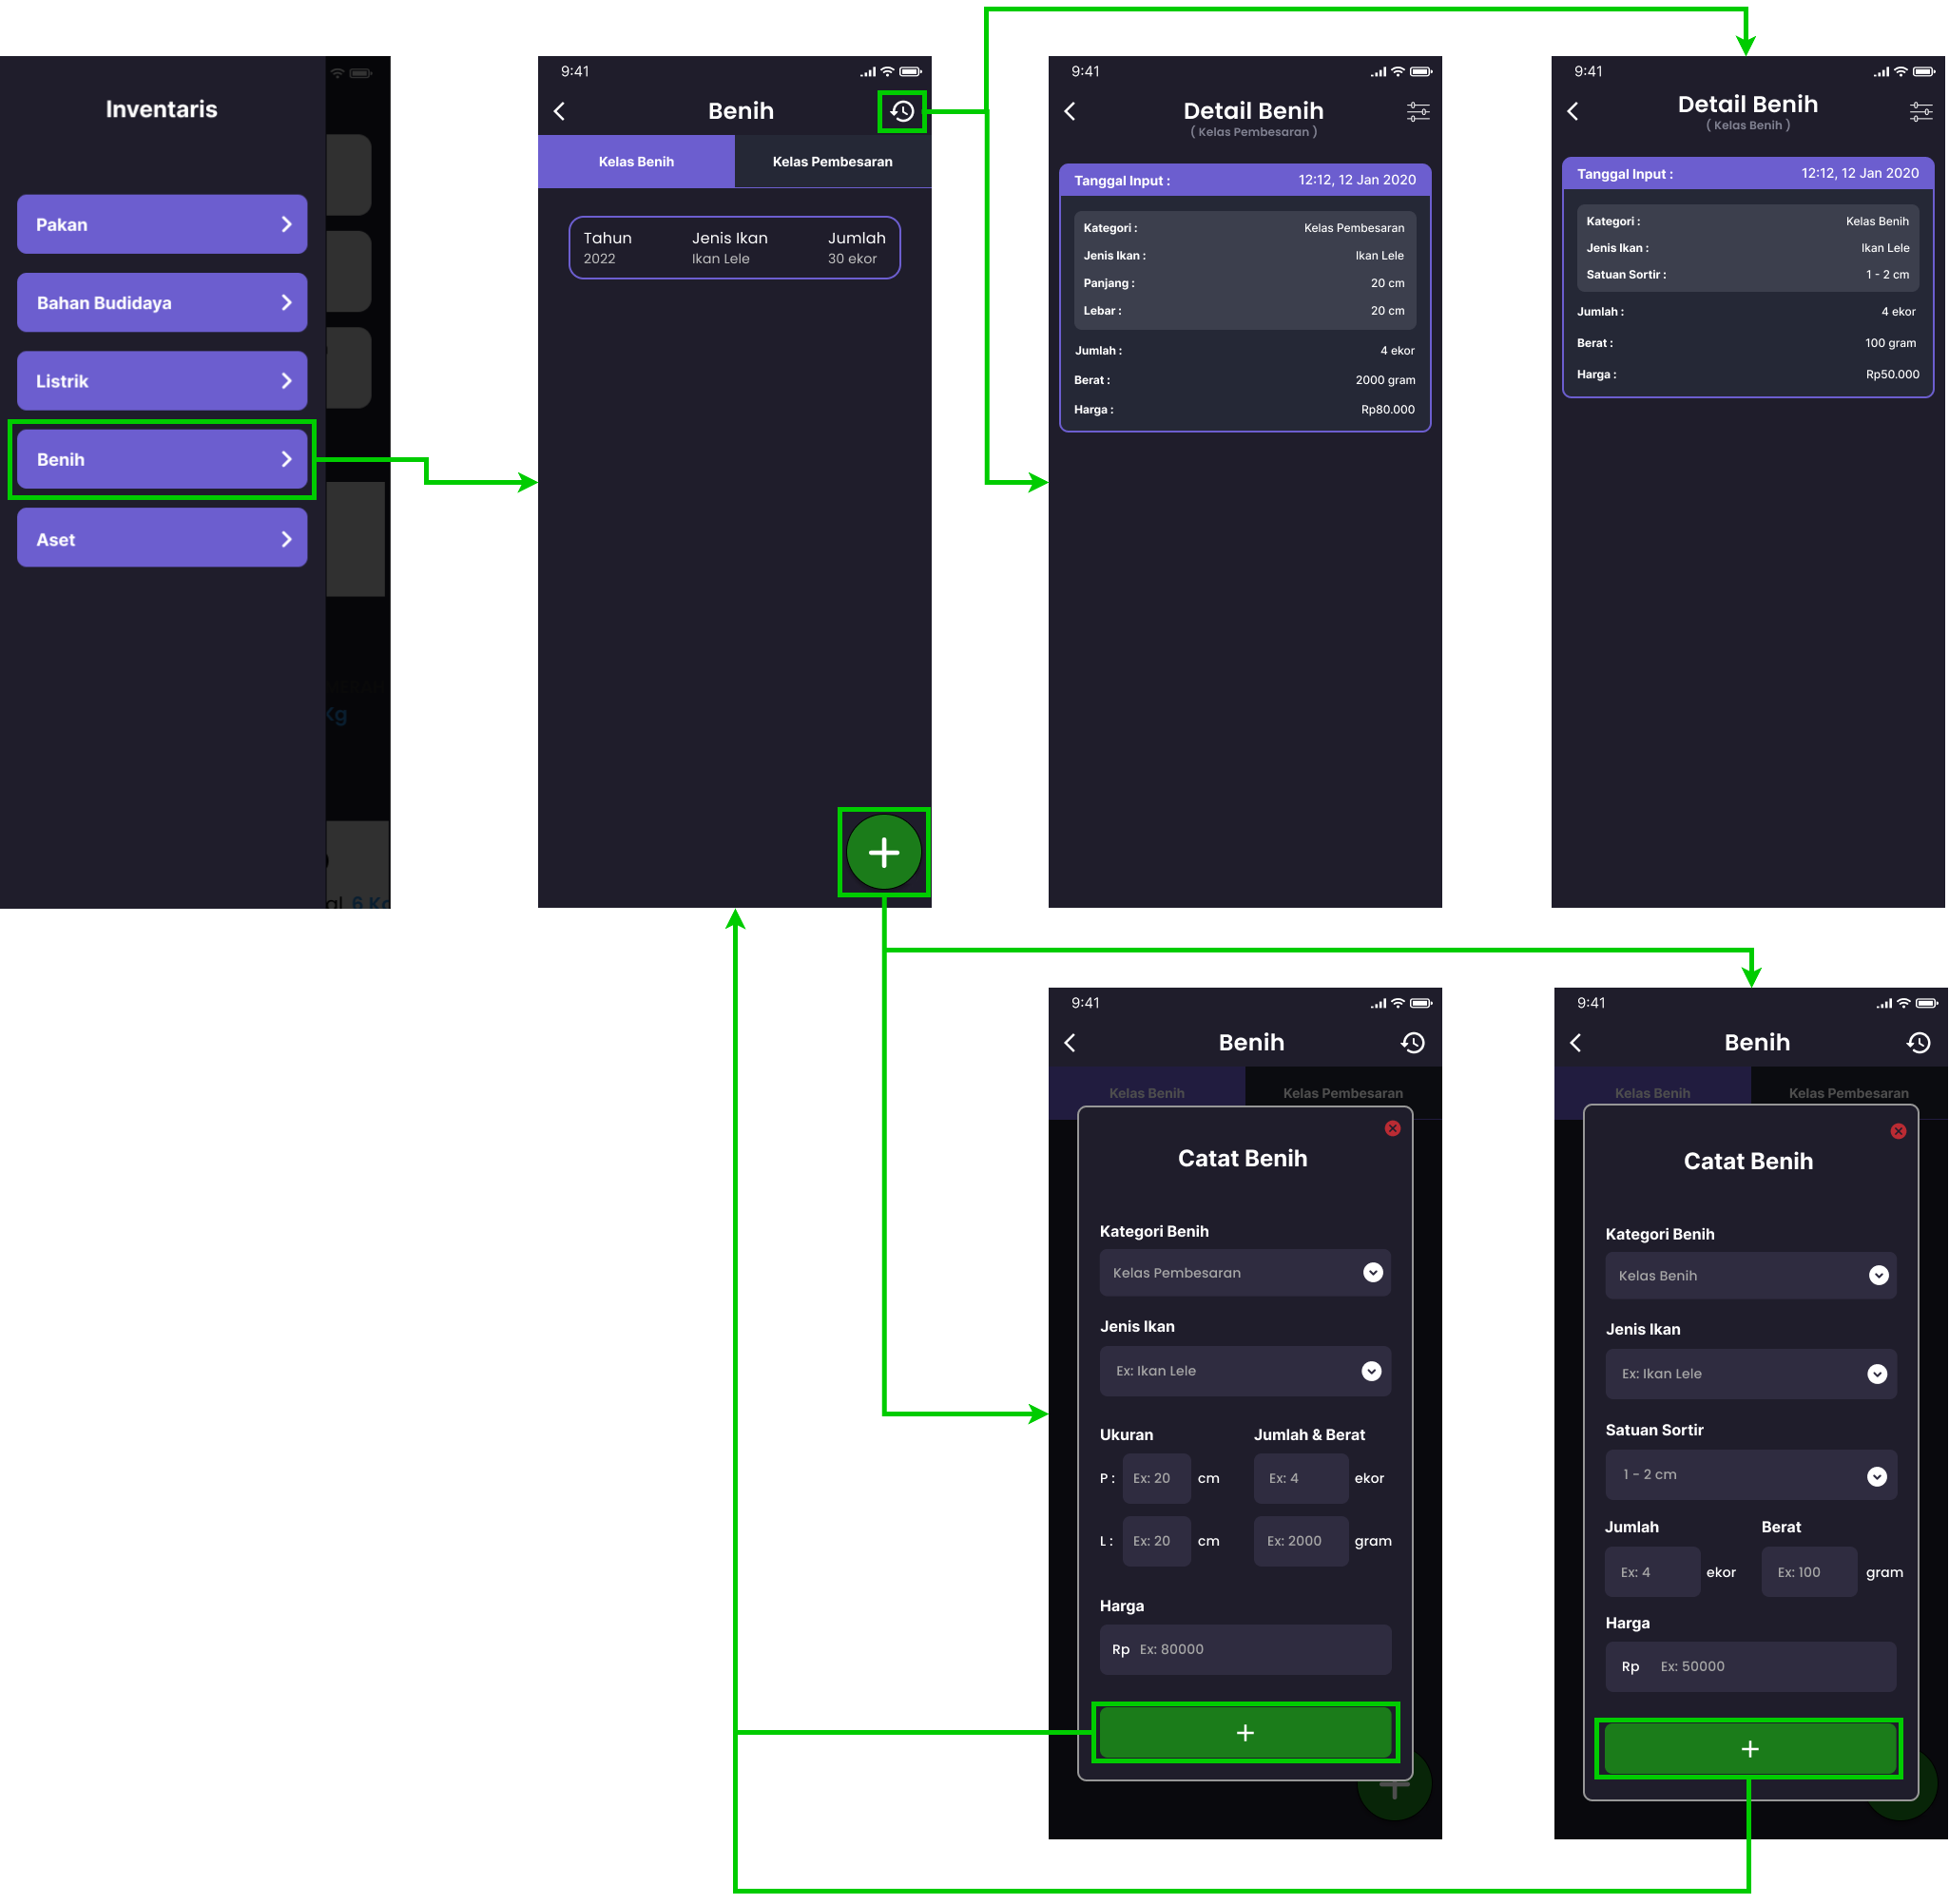
\includegraphics[width=1\textwidth]{gambar/sprint2/flow_seed.png}
		\caption{Alur Inventaris Benih}
	\end{figure}

	Pada \textbf{Gambar 4.22} merupakan alur dari inventaris benih. Pengguna akan memilih menu "Benih" dan masuk ke halaman data inventaris benih, kemudian tombol (+) akan menavigasikan pengguna ke halaman input benih dan tombol riwayat akan menavigasikan pengguna ke halaman detail input benih.

	\begin{figure}[H]
		\centering
		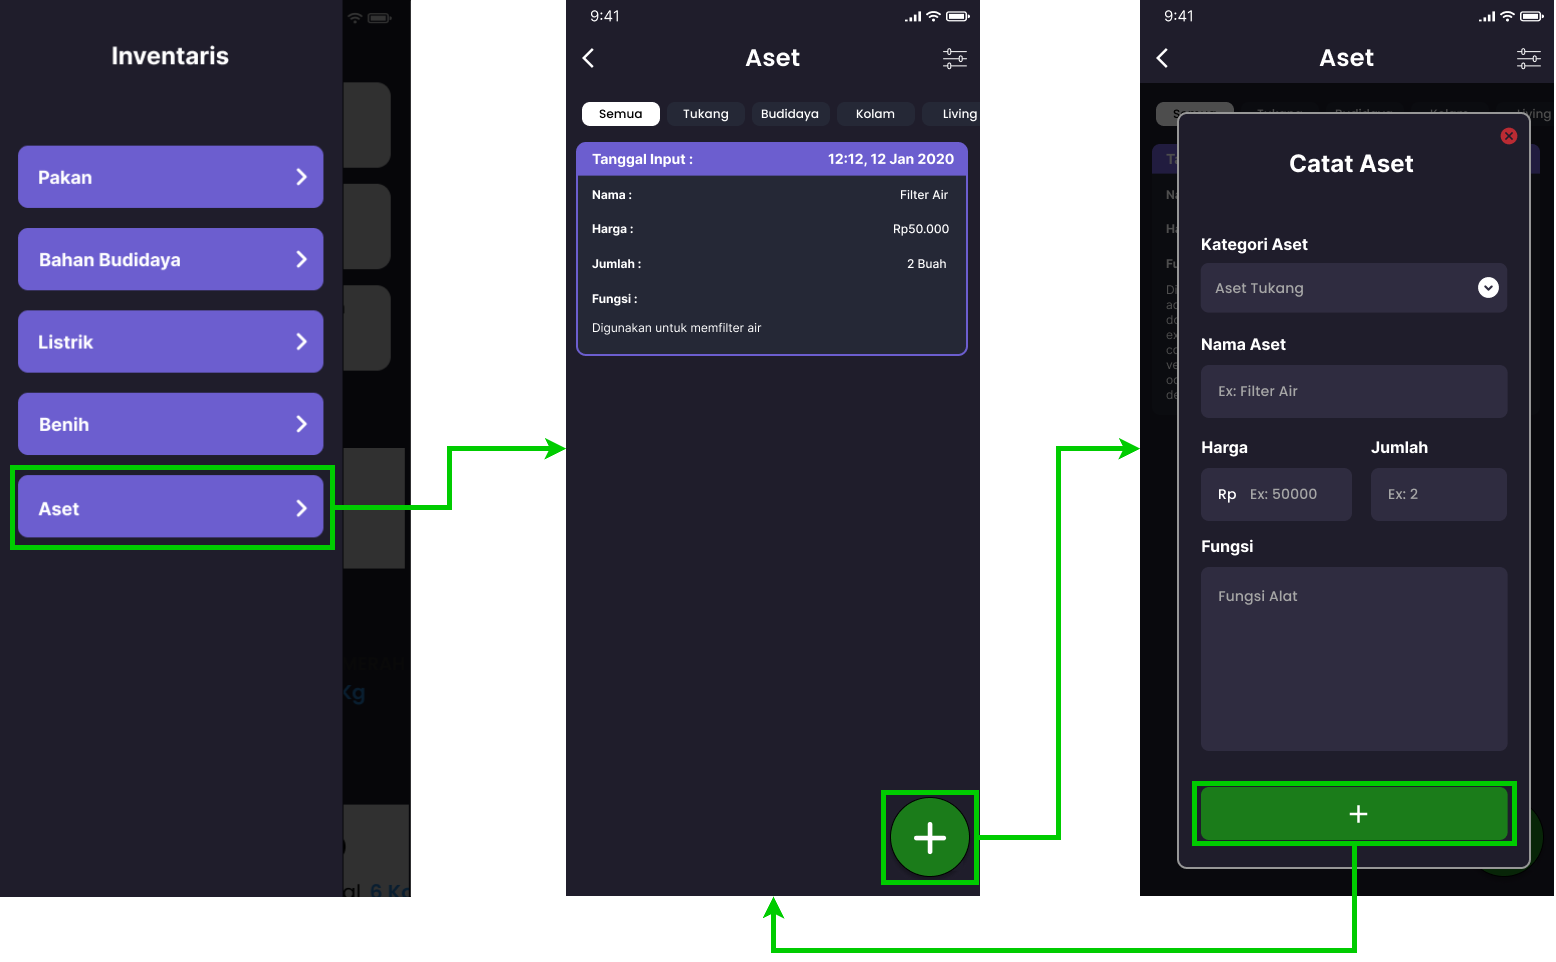
\includegraphics[width=1\textwidth]{gambar/sprint2/flow_asset.png}
		\caption{Alur Inventaris Aset}
	\end{figure}

	Pada \textbf{Gambar 4.23} merupakan alur dari inventaris aset. Pengguna akan memilih menu "Aset" dan masuk ke halaman data inventaris aset, kemudian tombol (+) akan menavigasikan pengguna ke halaman input aset.

	Seteleh semua alur telah selesai dibuat, selanjutnya merupakan perubahan skema database inventaris yang dapat dilihat pada \textbf{Gambar 4.24} berikut.

	\begin{figure}[H]
		\centering
		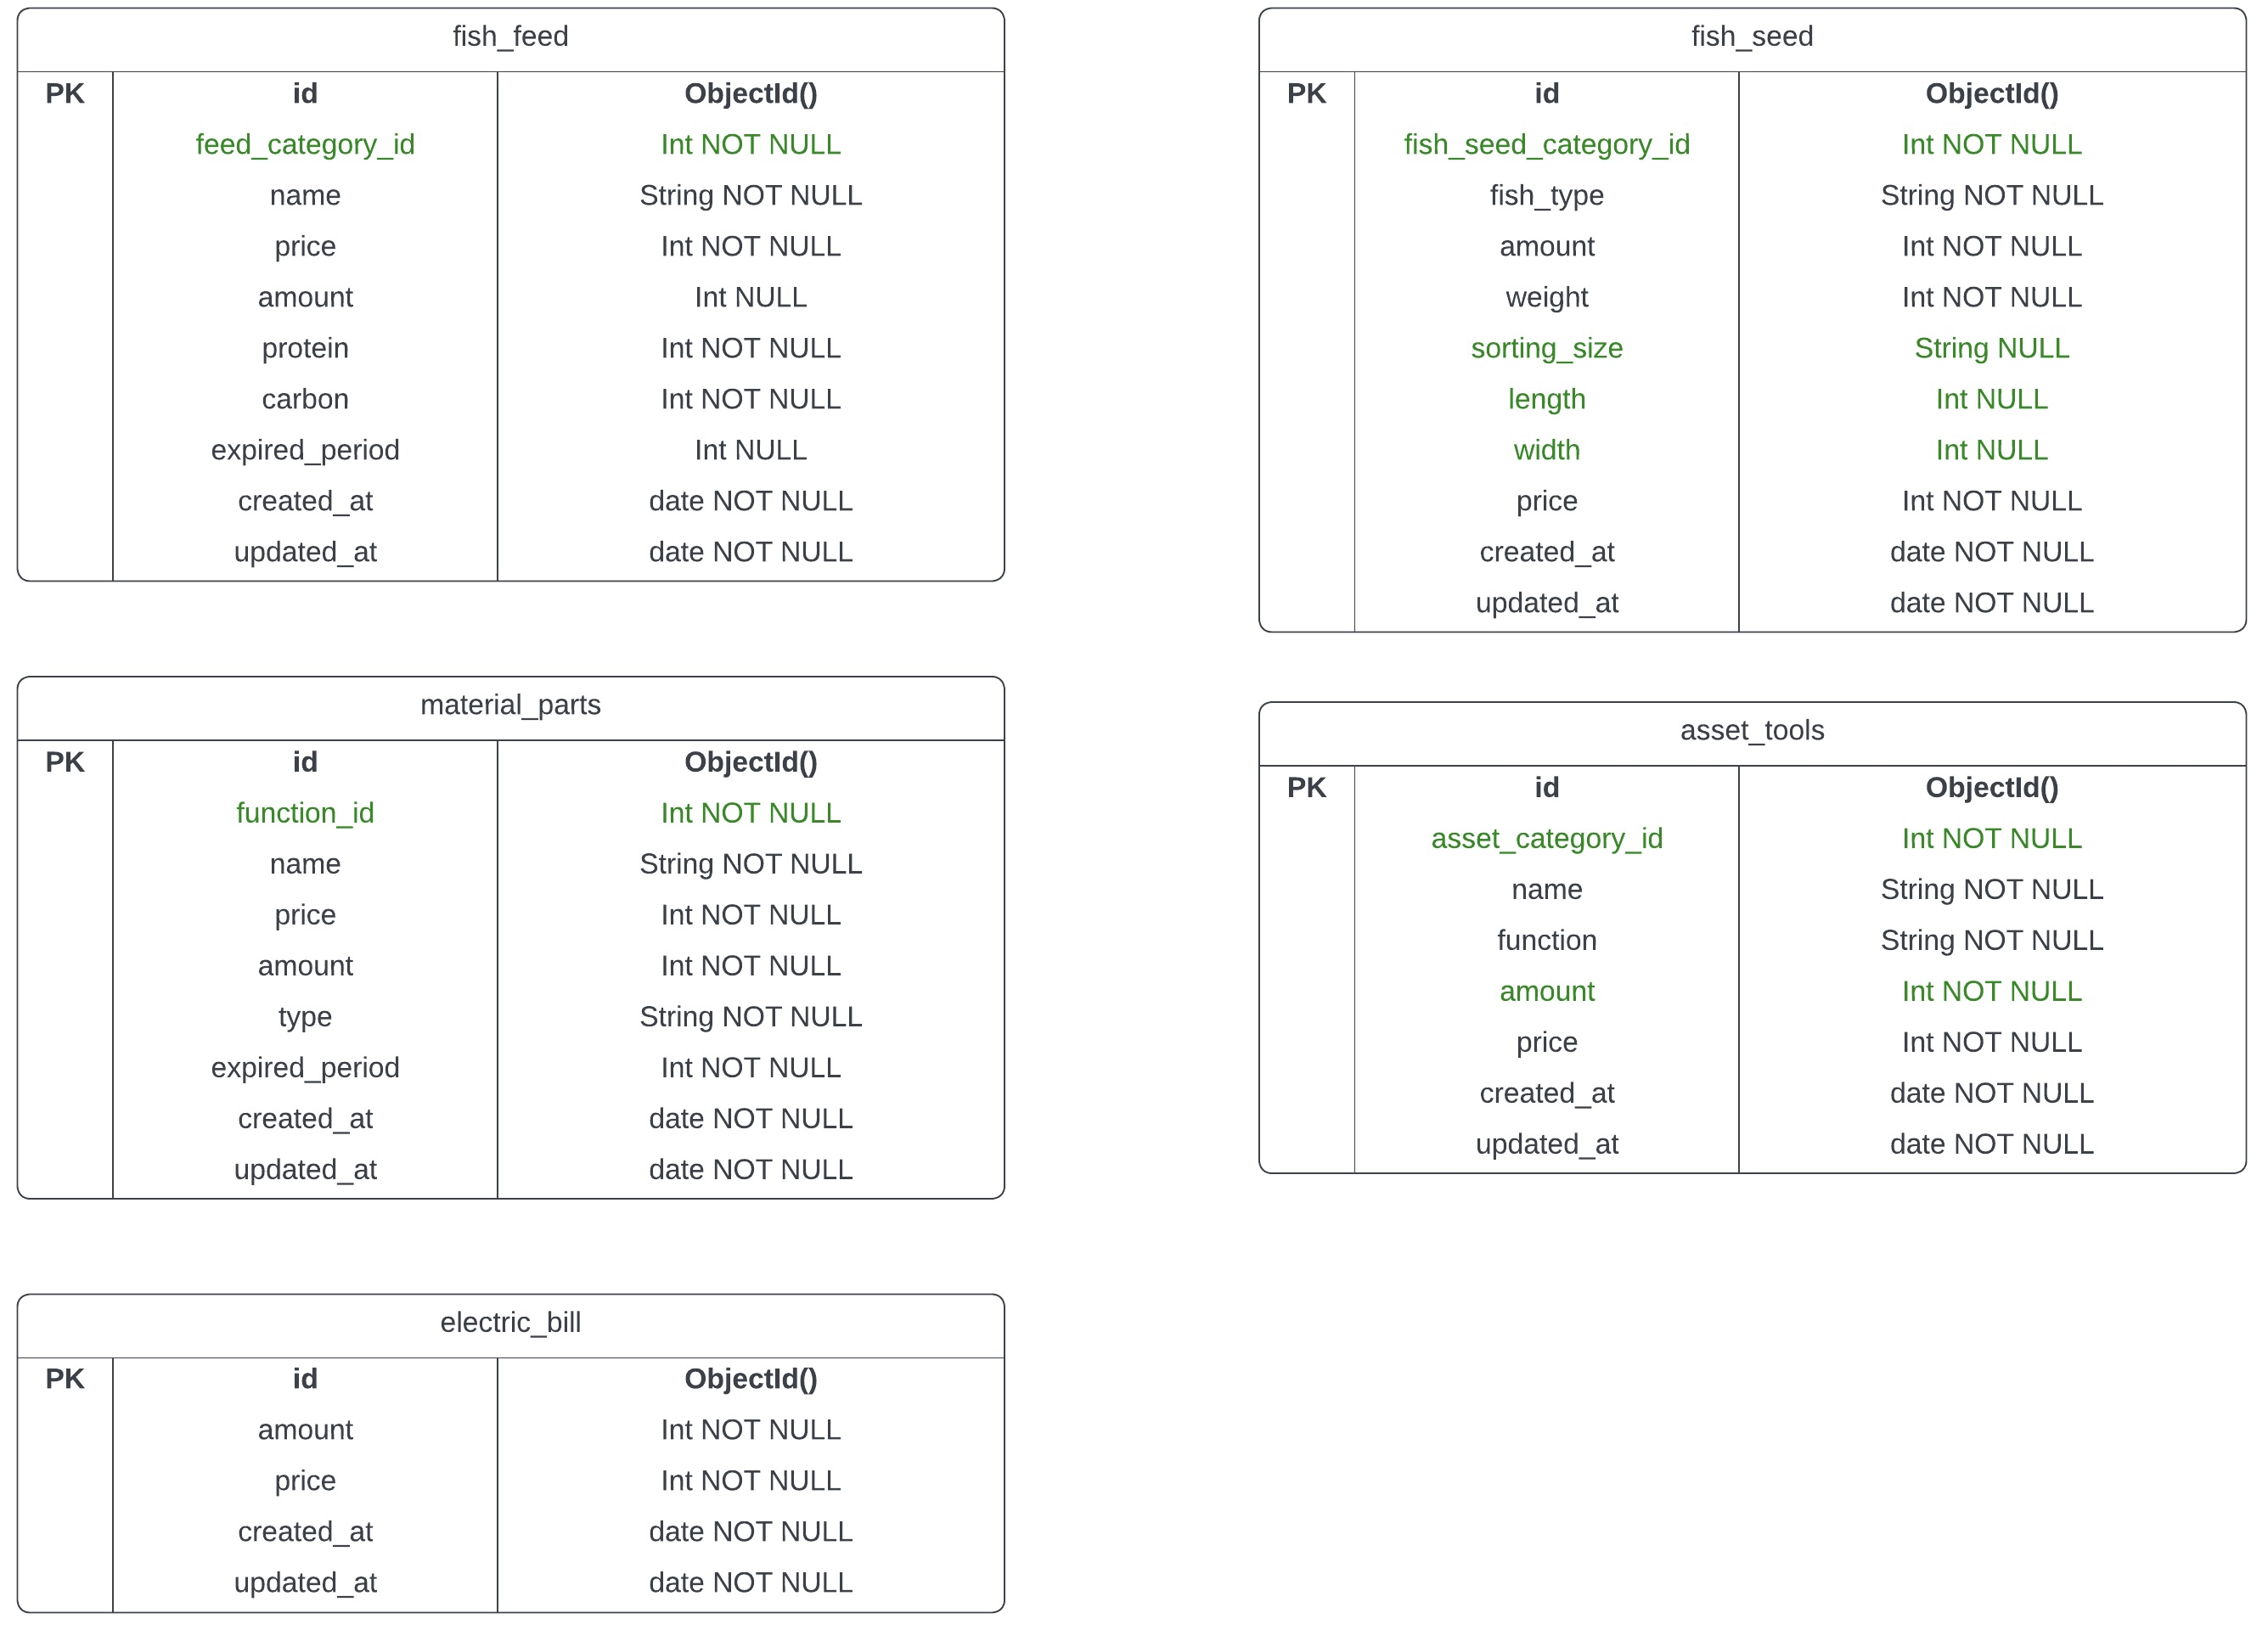
\includegraphics[width=1\textwidth]{gambar/sprint2/inventory_schema.jpeg}
		\caption{Update Skema Database Inventaris}
	\end{figure}

	Berdasarkan skema database inventaris tersebut, jika dibandingkan dengan skema database inventaris sebelumnya pada \textbf{Gambar 4.1} terdapat pembaruan pada bagian inventaris pakan, bahan budidaya, benih, dan aset.

	Pada skema database di inventaris pakan (fish\_feed), ditambahkan \textit{key} \textbf{feed\_category\_id} karena pada inventaris pakan diharuskan memilih kategori pakan yang akan dimasukkan. Untuk itu feed\_category\_id berperan untuk menampung jenis kategori pakan yang akan diinput. Sebelumnya jenis inventaris pakan tidak memiliki kategori, sehingga perlu ditambahkan \textit{key} baru untuk jenis data kategori tersebut.

	Kemudian, di skema database inventaris bahan budidaya (material\_parts) ditambahkan \textit{key} \textbf{function\_id} karena bahan budidaya dibagi menjadi dua fungsi yaitu perawatan air dan obat-obatan. Sebelumnya inventaris bahan budidaya tidak memiliki kategori, sehingga harus ditambahkan \textit{key} baru pada database untuk menampung jenis data tersebut.

	Lalu pada skema database inventaris benih ditambahkan \textit{key} \textbf{fish\_seed\_category\_id}, \textbf{sorting\_size}, \textbf{length}, serta \textbf{width}. \textit{key} tersebut ditambahkan karena pada benih dibagi menjadi dua jenis yaitu kelas benih dan kelas pembesaran. Masing-masing kategori memiliki jenis data pengukuran yang berbeda, pada kelas benih digunakan pengukuran satuan sortir dengan \textit{key} sorting\_size sementara kelas pembesaran digunakan pengukuran panjang dan lebar dengan \textit{key} \textit{length} dan \textit{width}. Sebelumnya untuk benih tidak terdapat kategori dan jenis ukuran benih sehingga \textit{key} baru diperlukan untuk menampung data tersebut.

	Terakhir terdapat perubahan pada skema database inventaris aset yaitu ditambahkan \textit{key} \textbf{asset\_category\_id} dan \textbf{amount}. Sebelumnya inventaris aset hanya menampung segala jenis aset yang digunakan pada musim budidaya tanpa adanya jenis kategori dan jumlah yang spesifik, namun di skema database sekarang dapat ditentukan jenis kategori pada aset dan berapa jumlah aset yang digunakan sehingga pemantauan aset yang digunakan menjadi lebih detail.

\subsection{Sprint 3}

	Sprint 3 dilaksanakan pada tanggal 10 Mei 2023 - 21 Juni 2023. Detail dari Sprint 3 ini adalah mengerjakan tugas yang ada pada Sprint 3 Backlog di tabel berikut.
		
	\begin{table}[H]	
		\begin{center}
			\caption{Sprint 3 Backlog}
			\label{tab:table20}
			\begin{tabular}{|c|c|m{13em}|c|}
			\hline
			\textbf{No} & \textbf{Stories} & \textbf{Task} & \textbf{Status} \\
			\hline
			1 & \multirow{2}{12em}{Fitur pencatatan inventaris} & - Design route untuk inventaris benih (dalam bentuk RESTful API) & Selesai \\
			&  & - Membuat halaman serta Integrasi RESTful API benih dengan Flutter & Selesai \\ 
			\hline
			2 & \multirow{2}{12em}{Fitur Aktivasi kolam dengan inventaris} & - Membuat tabel riwayat pemakaian benih & Selesai \\
			&  & - Design route dan penerapan dengan Flutter untuk riwayat pemakaian benih (dalam bentuk RESTful API) & Selesai \\ 
			\hline
			\end{tabular}
		\end{center}
	\end{table}

	Dalam proses Sprint ini, beberapa tahapan yang dilakukan adalah sebagai berikut :

	\begin{enumerate}
		\item Design route untuk inventaris benih (dalam bentuk RESTful API)
		
		Pada tugas ini, langkah pertama yang dilakukan adalah membuat sample route berupa url endpoint yang nantinya akan digunakan Flutter untuk berkomunikasi dengan backend. Hasilnya adalah sebagai berikut:

		\begin{figure}[H]
			\centering
			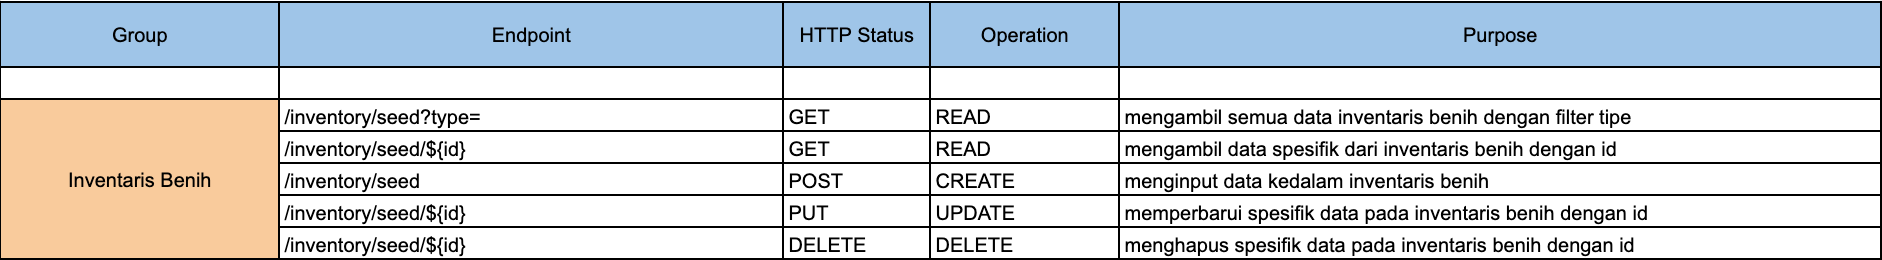
\includegraphics[width=1\textwidth]{gambar/sprint3/benih_route.png}
			\caption{Sample Route Benih}
		\end{figure}

		Kemudian, sebelum mengimplementasikan route tersebut dalam backend. Hal yang harus dilakukan adalah membuat model database dari inventaris benih berdasarkan skema database yang sudah dibuat pada Sprint 2. Berikut merupakan model inventaris benih pada Flask:

		\begin{itemize}
			\item Model Inventaris Benih
			\begin{lstlisting}
				class SeedInventory(db.Document):
					id_int = db.SequenceField(required=True)
					farm_id = db.ReferenceField(Farm, required=True)
					fish_seed_category = db.StringField(required=True)
					fish_type = db.StringField(required=True)
					brand_name = db.StringField(required=True)
					amount = db.IntField(required=True)
					weight = db.FloatField(default=0)
					width = db.StringField()
					price = db.IntField(required=True)
					total_price = db.IntField(required=True)
					image = db.StringField(required=True)
					created_at = db.DateTimeField(default=datetime.datetime.now)
					updated_at = db.DateTimeField(default=datetime.datetime.now)
			\end{lstlisting}
		\end{itemize}

		Setelah model dibuat, pengimplementasian model tersebut dalam Flask diperlukan bentuk class yang isinya mengandung fungsi-fungsi HTTP Request yang diperlukan. Berikut class hasil pengimplementasian model yang sudah dibuat sebelumnya sebagai berikut :

		\begin{enumerate}
			\item Mengambil semua data benih (HTTP Method - GET)
			
			Fungsi ini digunakan untuk menerima GET request dan akan meresepon dengan data yang ada pada database inventaris benih.
			
			\begin{lstlisting}
				class SeedInventoriesApi(Resource):
					@jwt_required()
					def get(self):
						try:
							current_user = get_jwt_identity()
							farm = str(current_user['farm_id'])
							farm_id = ObjectId(farm)
							
							type = request.args.get('type') if request.args.get('type') else ""
				
							pipeline = [
								{"$sort": {"id_int": 1}},
								{
									'$match': {
										"farm_id": farm_id,
										'fish_seed_category': {
											'$regex': type,
											'$options': 'i'
										}
									}
								},
							]
						
							testing = SeedInventory.objects.aggregate(pipeline)
							temp = list(testing)
							response = json.dumps({
								'status': 'success',
								'data': temp,
							}, default=str)
							return Response(response, mimetype="application/json", status=200)
						except Exception as e:
							response = {"message": e}
							response = json.dumps(response, default=str)
							return Response(response, mimetype="application/json", status=400)
			\end{lstlisting}

			Di fungsi tersebut terdapat variabel type yang berisi request.args.get yang digunakan untuk mengambil data parameter sebagai filter kepada database yang diambil. Pipeline pada fungsi ini berguna untuk menentukan secara spesifik bagaimana bentuk data yang akan diambil nanti dari database inventaris benih. 
			
			Jika tidak ada kendala dalam request data maka akan mendapatkan response status 200 yang berarti berhasil, jika tidak akan mendapatkan response status 400 yang berarti ada masalah saat melakukan request.

			\hfill \break
			
			\item Mengambil data benih secara spesifik berdasarkan ID benih (HTTP Method - GET)
			
			Fungsi ini digunakan untuk menerima GET request dan akan meresepon dengan data yang ada pada database inventaris benih secara spesifik sesuai dengan ID benih.
			
			\begin{lstlisting}
				class SeedInventoryApi(Resource):
					def get(self, id):
						try:
							pipeline = {"$match": {"id_int": int(id)}},
							testing = SeedInventory.objects.aggregate(pipeline)
							temp = list(testing)
							if len(temp) == 0:
								res = {"message": 'no data found'}
								response = json.dumps(res, default=str)
								return Response(response, mimetype="application/json", status=200)
							response = json.dumps({
								'status': 'success',
								'data': temp[0],
							}, default=str)
							return Response(response, mimetype="application/json", status=200)
						except Exception as e:
							response = {"message": e}
							response = json.dumps(response, default=str)
							return Response(response, mimetype="application/json", status=400)
			\end{lstlisting}

			\item Membuat data benih (HTTP Method - POST)
			
			Fungsi ini digunakan untuk membuat data benih di database dengan method POST.
			
			\begin{lstlisting}
				class SeedInventoriesApi(Resource):
					@jwt_required()
					def post(self):
						try:
							current_user = get_jwt_identity()
							farm = str(current_user['farm_id'])
							body = {
								"farm_id": farm,
								"fish_seed_category": request.form.get('fish_seed_category', None),
								"fish_type": request.form.get('fish_type', None),
								"brand_name": request.form.get('brand_name', None),
								"amount": request.form.get('amount', None),
								"weight": request.form.get('weight', None),
								"width": request.form.get('width', None),
								"price": request.form.get('price', None),
								"total_price": request.form.get('total_price', None),
								"image": request.form.get('image', None)
							}
							inventory = SeedInventory(**body).save()
							id = inventory.id
							res = {"message": "success add seed to inventory", "id": id, "data": body}
							response = json.dumps(res, default=str)
							return Response(response, mimetype="application/json", status=200)
						except Exception as e:
							response = {"message": str(e)}
							response = json.dumps(response, default=str)
							return Response(response, mimetype="application/json", status=400)
			\end{lstlisting}

			Di fungsi ini, terdapat body yang berisi parameter form data yang akan dikirim dari frontend dan sesuai dengan model yang ada pada inventaris benih.

			\item Memperbarui data benih secara spesifik berdasarkan ID benih (HTTP Method - PUT)
			
			Fungsi ini digunakan untuk memperbarui data benih berdasarkan ID benih di database dengan method PUT.
			
			\begin{lstlisting}
				class SeedInventoryApi(Resource):
					def put(self, id):
						try:
							body = {
								"id_int": int(id),
								"fish_seed_category": request.form.get('fish_seed_category', None),
								"fish_type": request.form.get('fish_type', None),
								"brand_name": request.form.get('brand_name', None),
								"amount": request.form.get('amount', None),
								"weight": request.form.get('weight', None),
								"width": request.form.get('width', None),
								"price": request.form.get('price', None),
								"total_price": request.form.get('total_price', None),
								"image": request.form.get('image', None)
							}
							inventory = SeedInventory.objects.get(id_int = int(id)).update(**body)
							response = {"message": "success update seed inventory", "data": body}
							response = json.dumps(response, default=str)
							return Response(response, mimetype="application/json", status=200)
						except Exception as e:
							response = {"message": str(e)}
							response = json.dumps(response, default=str)
							return Response(response, mimetype="application/json", status=400)
			\end{lstlisting}

			Fungsi ini kurang lebih sama seperti method POST karena memerlukan body yang sejenis, body ini nantinya yang akan dihubungkan ke database inventaris benih.

			\item Menghapus data benih secara spesifik berdasarkan ID benih (HTTP Method - DELETE)
			
			Fungsi ini digunakan untuk menghapus data benih berdasarkan ID benih di database dengan method DELETE.
			
			\begin{lstlisting}
				class SeedInventoryApi(Resource):
					def delete(self, id):
						try:
							inventory = SeedInventory.objects.get(id_int = int(id)).delete()
							response = {"message": "success delete seed inventory"}
							response = json.dumps(response, default=str)
							return Response(response, mimetype="application/json", status=200)
						except Exception as e:
							response = {"message": str(e)}
							response = json.dumps(response, default=str)
							return Response(response, mimetype="application/json", status=400)
			\end{lstlisting}
		\end{enumerate}

		Setelah class selesai dibuat, diperlukan route yang digunakan untuk menyambungkan ke class tersebut. Route ini dapat dilihat pada sample route yang sudah dibuat sebelumnya. Berikut cara penyambungan route terhadap class pada Flask :

		\begin{lstlisting}
			# seed inventory
			api.add_resource(SeedInventoriesApi, '/api/inventory/seed')
			api.add_resource(SeedInventoryApi, '/api/inventory/seed/<id>')
		\end{lstlisting}

		Route tersebut nantinya yang akan digunakan Flutter untuk berkomunikasi pada backend sesuai dengan HTTP Request yang ada pada class tersebut.

		\item Membuat halaman serta Integrasi RESTful API benih dengan Flutter
		
		Pada Flutter, untuk berkomunikasi pada backend diperlukan package HTTP yang perlu ditambahkan terlebih dahulu.
		
		\begin{figure}[H]
			\centering
			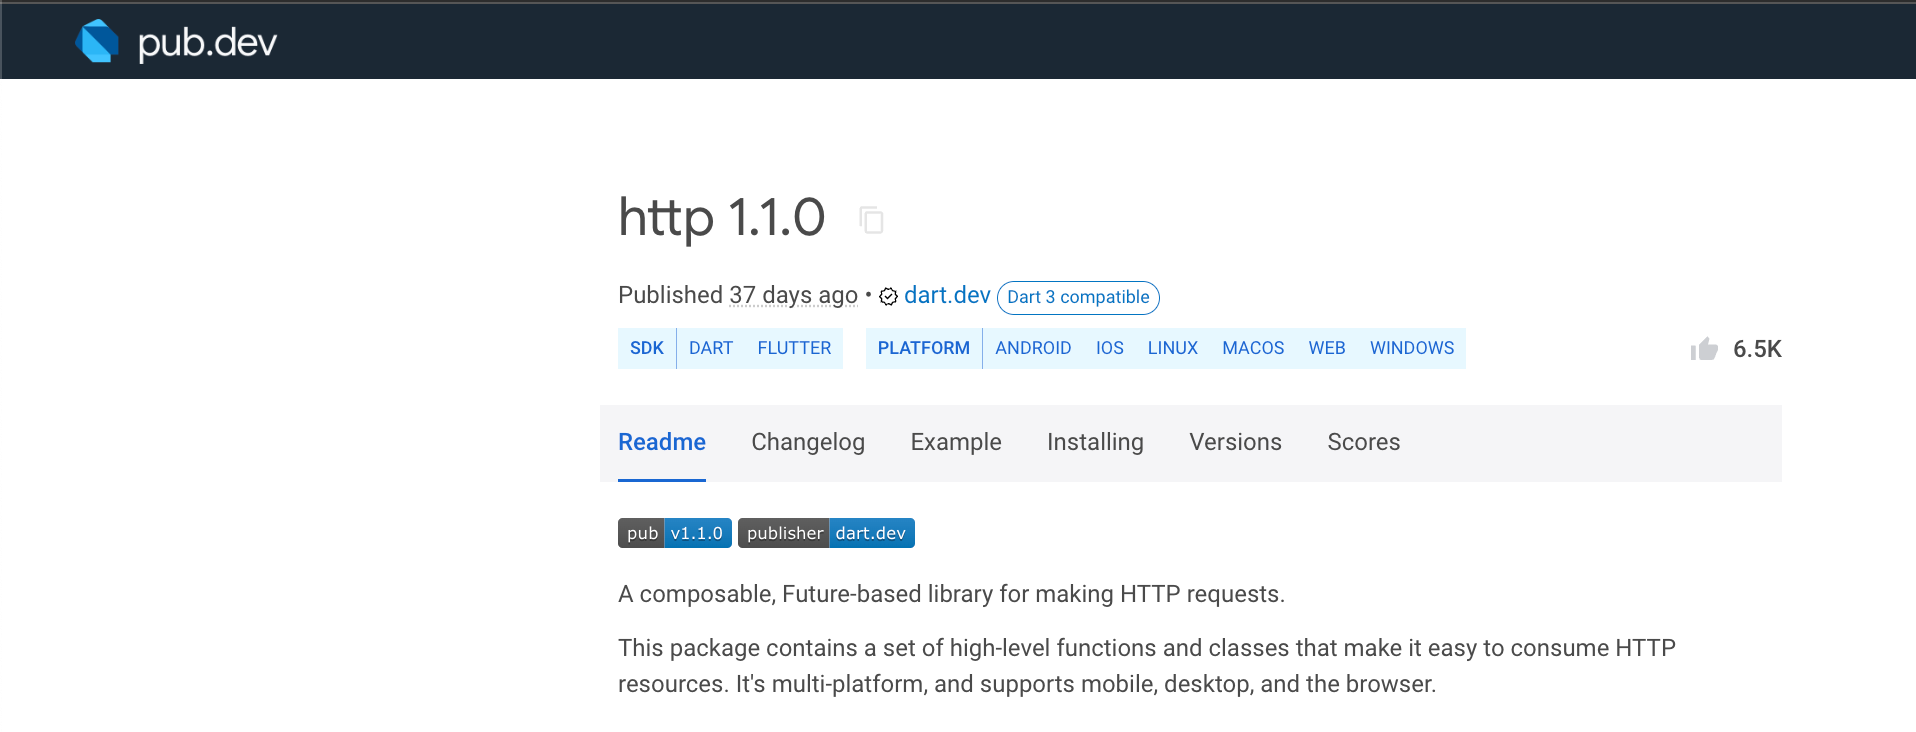
\includegraphics[width=1\textwidth]{gambar/sprint3/http_pub.png}
			\caption{Package HTTP untuk Flutter}
		\end{figure}

		\begin{figure}[H]
			\centering
			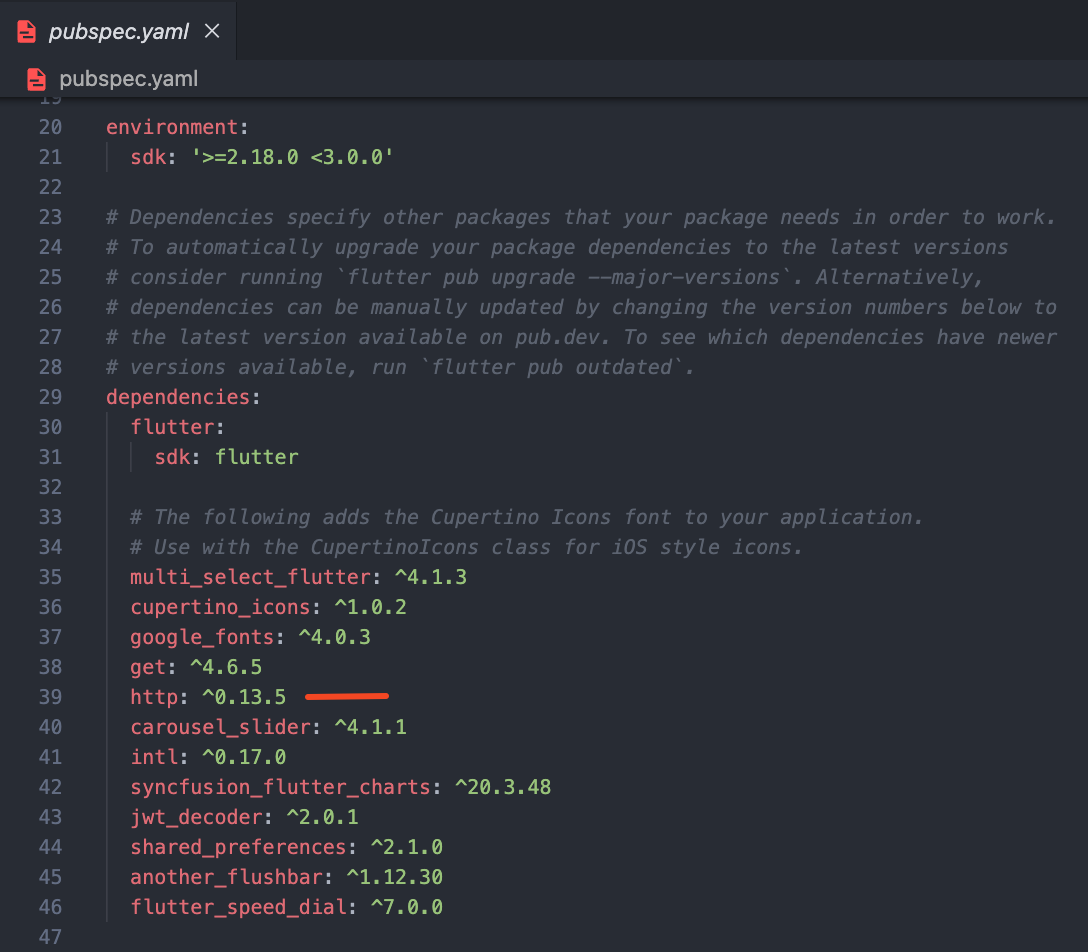
\includegraphics[width=0.6\textwidth]{gambar/sprint3/pubspec_http.png}
			\caption{Penambahan package HTTP pada Flutter}
		\end{figure}

		Setelah package HTTP ter-install, dibuatlah controller yang berisi fungsi-fungsi HTTP request yang sesuai dengan class route pada backend.

		Untuk keseluruhan fungsi HTTP request pada Flutter, dapat dilihat pada baris kode dibawah ini.

		\begin{enumerate}
			\item Mengambil semua data benih (HTTP Method - GET) 
			
			Fungsi ini digunakan untuk mengambil semua data benih, baik itu jenis benih ataupun pembesaran dari segala jenis ikan.

			\begin{lstlisting}
				Future getAllSeedData(String type) async {
					SharedPreferences prefs = await SharedPreferences.getInstance();
					String token = prefs.getString('token').toString();

					seedList.value.data!.clear();
					nameHistoryList.clear();
					nameHistoryList.add('Semua');
					listMas.clear();
					listNilaHitam.clear();
					listNilaMerah.clear();
					listPatin.clear();
					listLele.clear();
					resetVariables();
					isLoadingPage.value = true;

					var headers = {'Authorization': 'Bearer $token'};
					final response = await http.get(
					Uri.parse('${Urls.invSeed}?type=$type'),
					headers: headers,
					);

					try {
					if (response.statusCode == 200) {
						InventarisBenihModel res =
							InventarisBenihModel.fromJson(jsonDecode(response.body));

						seedList.value = res;

						for (var i in seedList.value.data!) {
						nameHistoryList.add(i.brandName.toString());
						}

						for (var i in seedList.value.data!) {
						if (i.fishType == 'Lele') {
							listLele.add({
							'id': i.idInt,
							'seed_id': i.sId,
							'fishName': i.brandName,
							});

							selectedLele.value = listLele[0];
						}
						if (i.fishType == 'Nila Hitam') {
							listNilaHitam.add({
							'id': i.idInt,
							'seed_id': i.sId,
							'fishName': i.brandName,
							});

							selectedNilaHitam.value = listNilaHitam[0];
						}
						if (i.fishType == 'Nila Merah') {
							listNilaMerah.add({
							'id': i.idInt,
							'seed_id': i.sId,
							'fishName': i.brandName,
							});

							selectedNilaMerah.value = listNilaMerah[0];
						}
						if (i.fishType == 'Patin') {
							listPatin.add({
							'id': i.idInt,
							'seed_id': i.sId,
							'fishName': i.brandName,
							});

							selectedPatin.value = listPatin[0];
						}
						if (i.fishType == 'Mas') {
							listMas.add({
							'id': i.idInt,
							'seed_id': i.sId,
							'fishName': i.brandName,
							});

							selectedMas.value = listMas[0];
						}
						}

						selectedNameHistory.value = nameHistoryList[0];
					}
					// inspect(listLele);
					} catch (e) {
					throw Exception(e);
					}
					isLoadingPage.value = false;
				}
			\end{lstlisting}

			Parameter yang digunakan fungsi ini adalah type, type disini mewakili kategori benih yang ingin diambil. Pada proses pengambilan data benih, benih disimpan didalam variabel masing-masing yang diinisialsasikan sebagai list. Hasil dari request tersebut ditampung dalam variabel res yang merepresentasikan model inventaris benih.

			\item Mengambil data benih secara spesifik berdasarkan ID benih (HTTP Method - GET)
			
			Fungsi ini digunakan untuk mengambil data benih secara spesifik berdasarkan ID benih nya.
			
			\begin{lstlisting}
				Future getSeedDataByID(int id, Function() doAfter) async {
					isLoadingDetail.value = true;
					final response = await http.get(Uri.parse('${Urls.invSeed}/$id'));

					try {
					if (response.statusCode == 200) {
						DetailInventarisBenihModel res =
							DetailInventarisBenihModel.fromJson(jsonDecode(response.body));

						seedCategory.value = res.data!.fishSeedCategory.toString();
						fishCategory.value = res.data!.fishType.toString();
						sortSize.value = res.data!.width.toString();
						fishName.value = seedCategory.value == 'Benih'
							? '${fishCategory.value}${sortSize.value.split(' ')[0].replaceAll('-', '')}'
							: '${fishCategory.value}${fishWeight.text.split(' ')[0]}';
						fishAmount.text = res.data!.amount.toString();
						fishWeight.text = res.data!.weight!.toStringAsFixed(2);
						fishPrice.text = res.data!.price.toString();
						fishPriceTotal.text = res.data!.totalPrice.toString();
						fishImage.value = res.data!.image.toString();
					}
					doAfter();
					} catch (e) {
					throw Exception(e);
					}
					isLoadingDetail.value = false;
				}
			\end{lstlisting}

			Paramter fungsi ini tentunya adalah ID benih yang digunakan pada endpoint. Hasil dari request tersebut ditampung dalam variabel res yang merepresentasikan model detail inventaris benih dan masing-masing response diwakili satu per satu oleh variabel yang sesuai.

			\item Membuat data benih (HTTP Method - POST)
			
			Fungsi ini digunakan untuk membuat data benih yang akan dikirimkan ke database.

			\begin{lstlisting}
				Future postSeedData(Function() doAfter) async {
					var map = <String, dynamic>{};

					SharedPreferences prefs = await SharedPreferences.getInstance();
					String token = prefs.getString('token').toString();
					var headers = {'Authorization': 'Bearer $token'};

					map['fish_seed_category'] = seedCategory.value;
					map['fish_type'] = fishCategory.value;
					map['brand_name'] = seedCategory.value == 'Benih'
						? '${fishCategory.value.replaceAll(' ', '')}${sortSize.value.split(' ')[0]}'
						: '${fishCategory.value.replaceAll(' ', '')}${fishWeight.text.replaceAll(',', '.').split('.')[0]}';
					map['amount'] = fishAmount.text == '' ? '0' : fishAmount.text;
					map['weight'] =
						fishWeight.text == '' ? '0' : fishWeight.text.replaceAll(',', '.');
					map['width'] = seedCategory.value == 'Benih' ? sortSize.value : "";
					map['price'] = fishPrice.text == '' ? '0' : fishPrice.text;
					map['total_price'] = fishPriceTotal.text == '' ? '0' : fishPriceTotal.text;
					map['image'] = fishImage.value;

					isLoadingPost.value = true;

					inspect(map);

					try {
					await http.post(
						Uri.parse(Urls.invSeed),
						body: map,
						headers: headers,
					);
					doAfter();
					} catch (e) {
					throw Exception(e);
					}
					isLoadingPost.value = false;
				}
			\end{lstlisting}

			Untuk mengirim data body ke database, di Flutter menggunakan map untuk merepresentasikan value yang akan diterima pada backend nantinya. Jika value body tidak sesuai dengan yang ada di model backend, maka backend akan meresepon error dan data tidak dapat masuk ke database.

			\item Memperbarui data benih secara spesifik (HTTP Method - PUT)
			
			Fungsi ini digunakan untuk memperbarui data benih secara spesifik berdasarkan ID benih.

			\begin{lstlisting}
				Future updateSeedData(int id, Function() doAfter) async {
					var map = <String, dynamic>{};

					map['fish_seed_category'] = seedCategory.value;
					map['fish_type'] = fishCategory.value;
					map['brand_name'] = seedCategory.value == 'Benih'
						? '${fishCategory.value.replaceAll(' ', '')}${sortSize.value.split(' ')[0]}'
						: '${fishCategory.value.replaceAll(' ', '')}${fishWeight.text.replaceAll(',', '.').split('.')[0]}';
					map['amount'] = fishAmount.text == '' ? '0' : fishAmount.text;
					map['weight'] =
						fishWeight.text == '' ? '0' : fishWeight.text.replaceAll(',', '.');
					map['width'] = seedCategory.value == 'Benih' ? sortSize.value : "";
					map['price'] = fishPrice.text == '' ? '0' : fishPrice.text;
					map['total_price'] = fishPriceTotal.text == '' ? '0' : fishPriceTotal.text;
					map['image'] = fishImage.value;

					isLoadingPost.value = true;

					try {
					inspect(map);
					await http.put(
						Uri.parse('${Urls.invSeed}/$id'),
						body: map,
					);
					doAfter();
					} catch (e) {
					throw Exception(e);
					}
					isLoadingPost.value = false;
				}
			\end{lstlisting}

			Fungsi ini kurang lebih sama seperti fungsi POST request, bedanya hanya method nya saja. Untuk memperbarui data, digunakan method PUT dan value yang diterima merupakan body yang sudah di map.

			\item Menghapus data benih secara spesifik (HTTP Method - DELETE)
			
			Fungsi ini digunakan untuk menghapus data benih secara spesifik sesuai dengan ID benih.
			
			\begin{lstlisting}
				Future deleteSeedData(int id, Function() doAfter) async {
					isLoadingDelete.value = true;
					try {
					  await http.delete(
						Uri.parse(
						  '${Urls.invSeed}/$id',
						),
						headers: {
						  'Content-Type': 'application/json; charset=UTF-8',
						},
					  );
					  doAfter();
					} catch (e) {
					  throw Exception(e);
					}
					isLoadingDelete.value = false;
				  }
			\end{lstlisting}
		\end{enumerate}

		Parameter yang digunakan pada fungsi ini adalah ID benih dan method HTTP yang digunakan adalah DELETE.

		Setelah fungsi diatas sudah berjalan, diperlukan layout pada Flutter yang nantinya akan ditampilkan kepada user sehingga user dapat menggunakan aplikasi untuk fitur inventaris benih. Layout ini nantinya akan diintegrasikan dengan fungsi-fungsi HTTP request pada controller inventaris benih. Berikut layout atau tampilan dari inventaris benih. Untuk code dapat dilihat pada halaman Lampiran.

		\begin{figure}[H]
			\minipage{0.32\textwidth}
				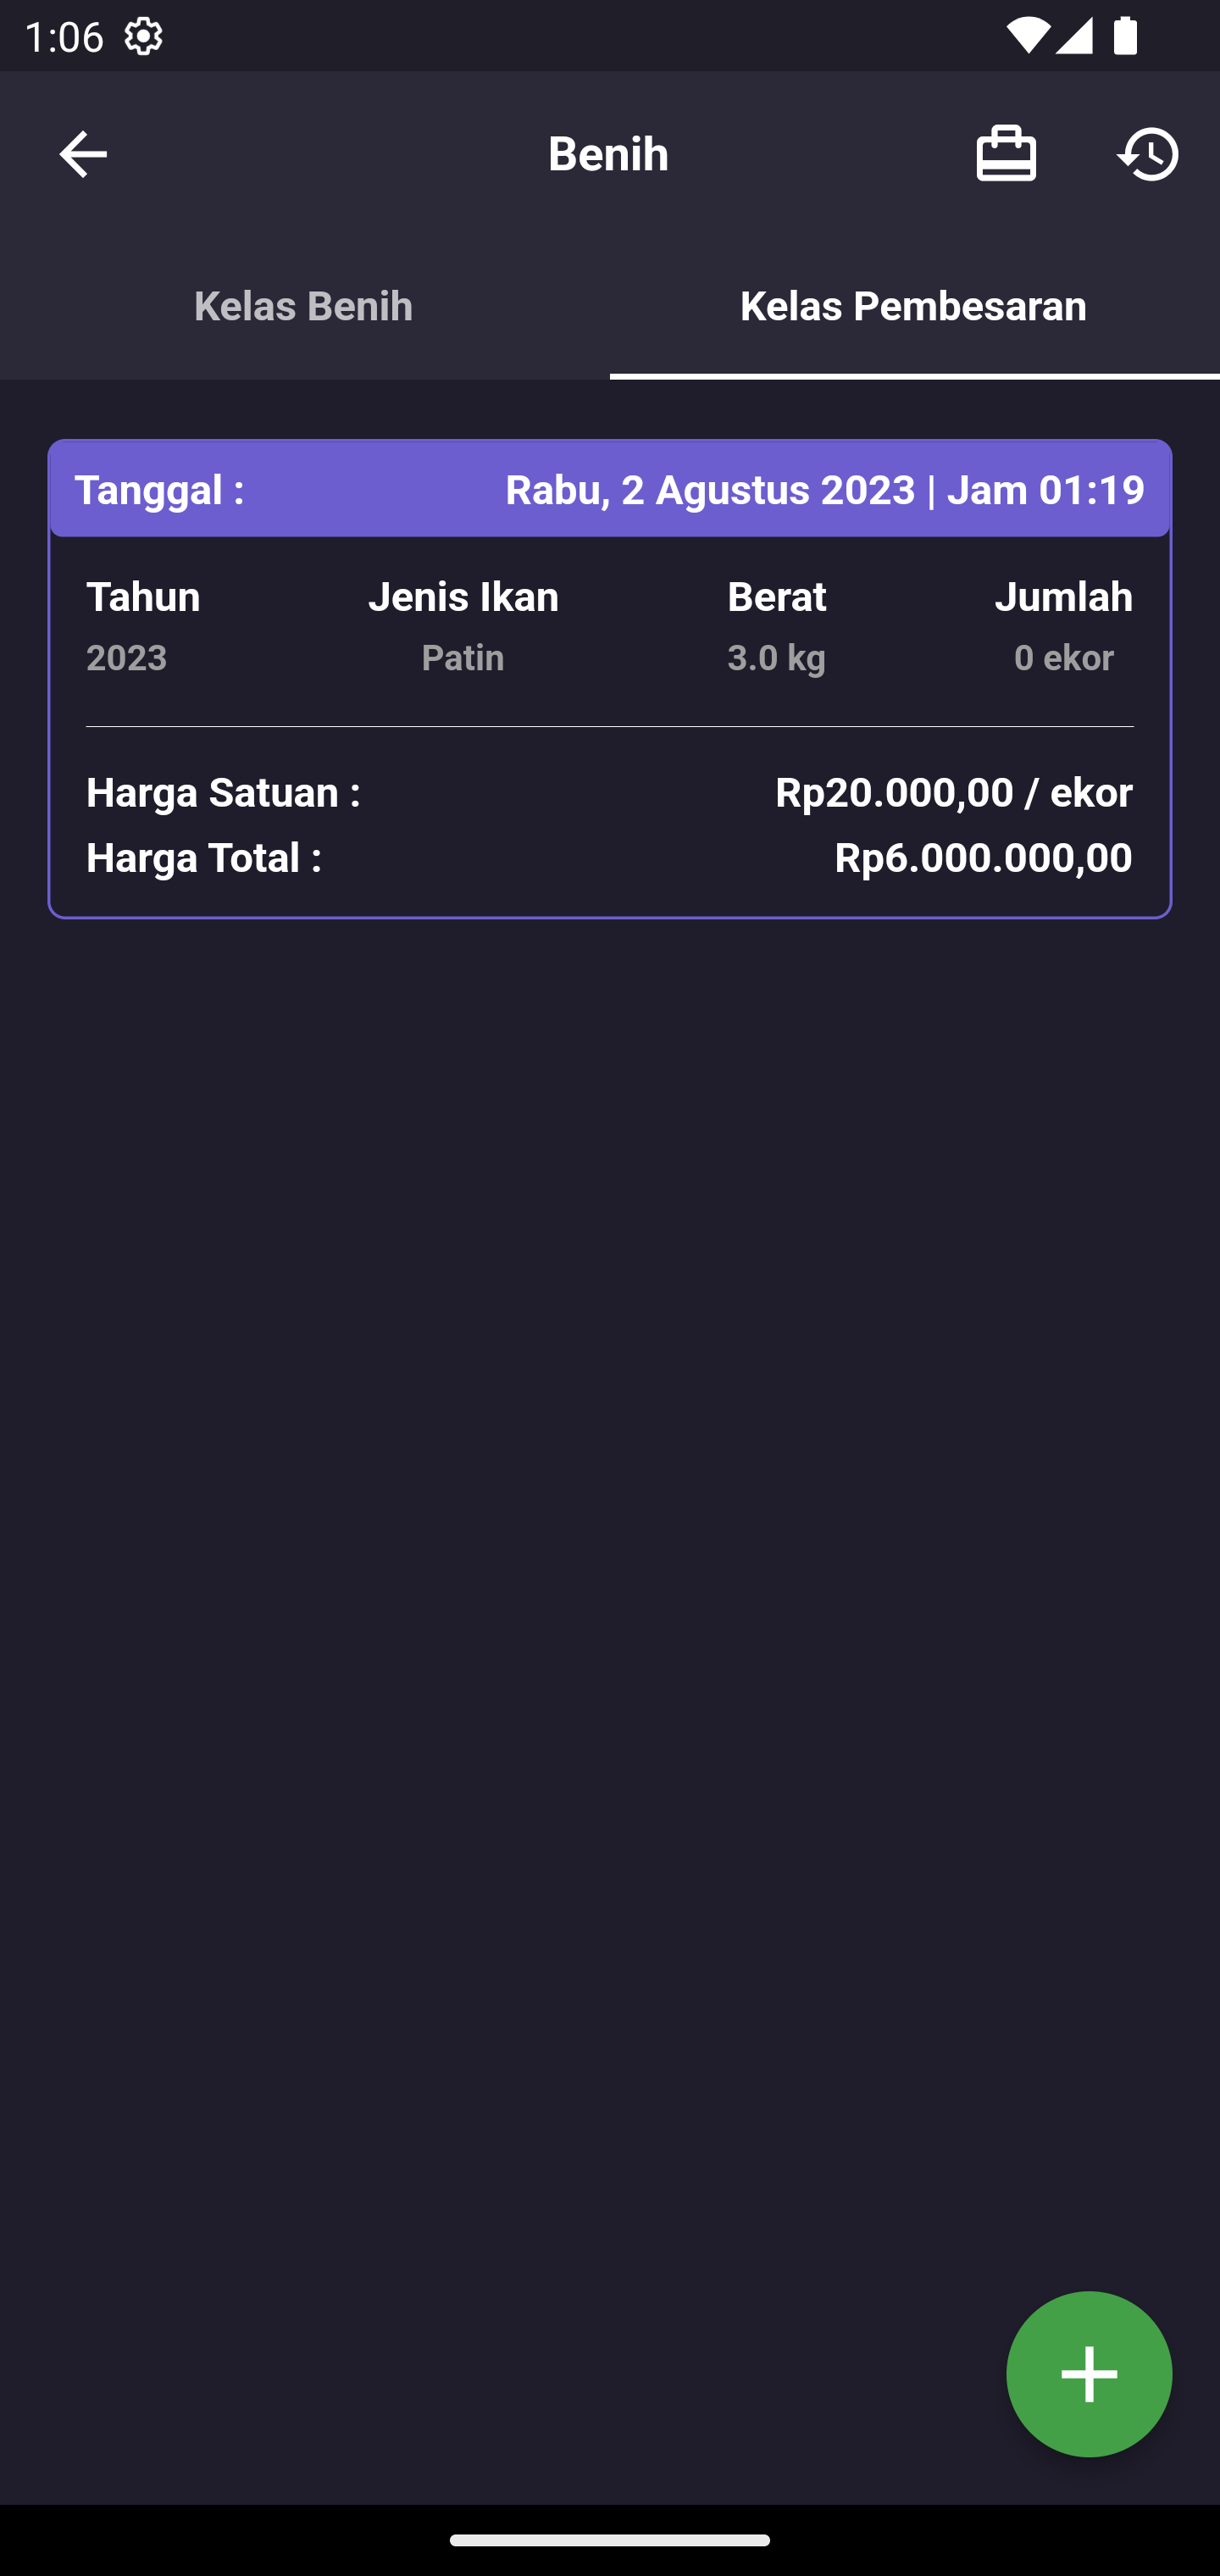
\includegraphics[width=\linewidth]{gambar/sprint3/benih_1.png}
				\caption{Halaman Inventaris Benih}
			\endminipage\hfill
			\minipage{0.32\textwidth}
				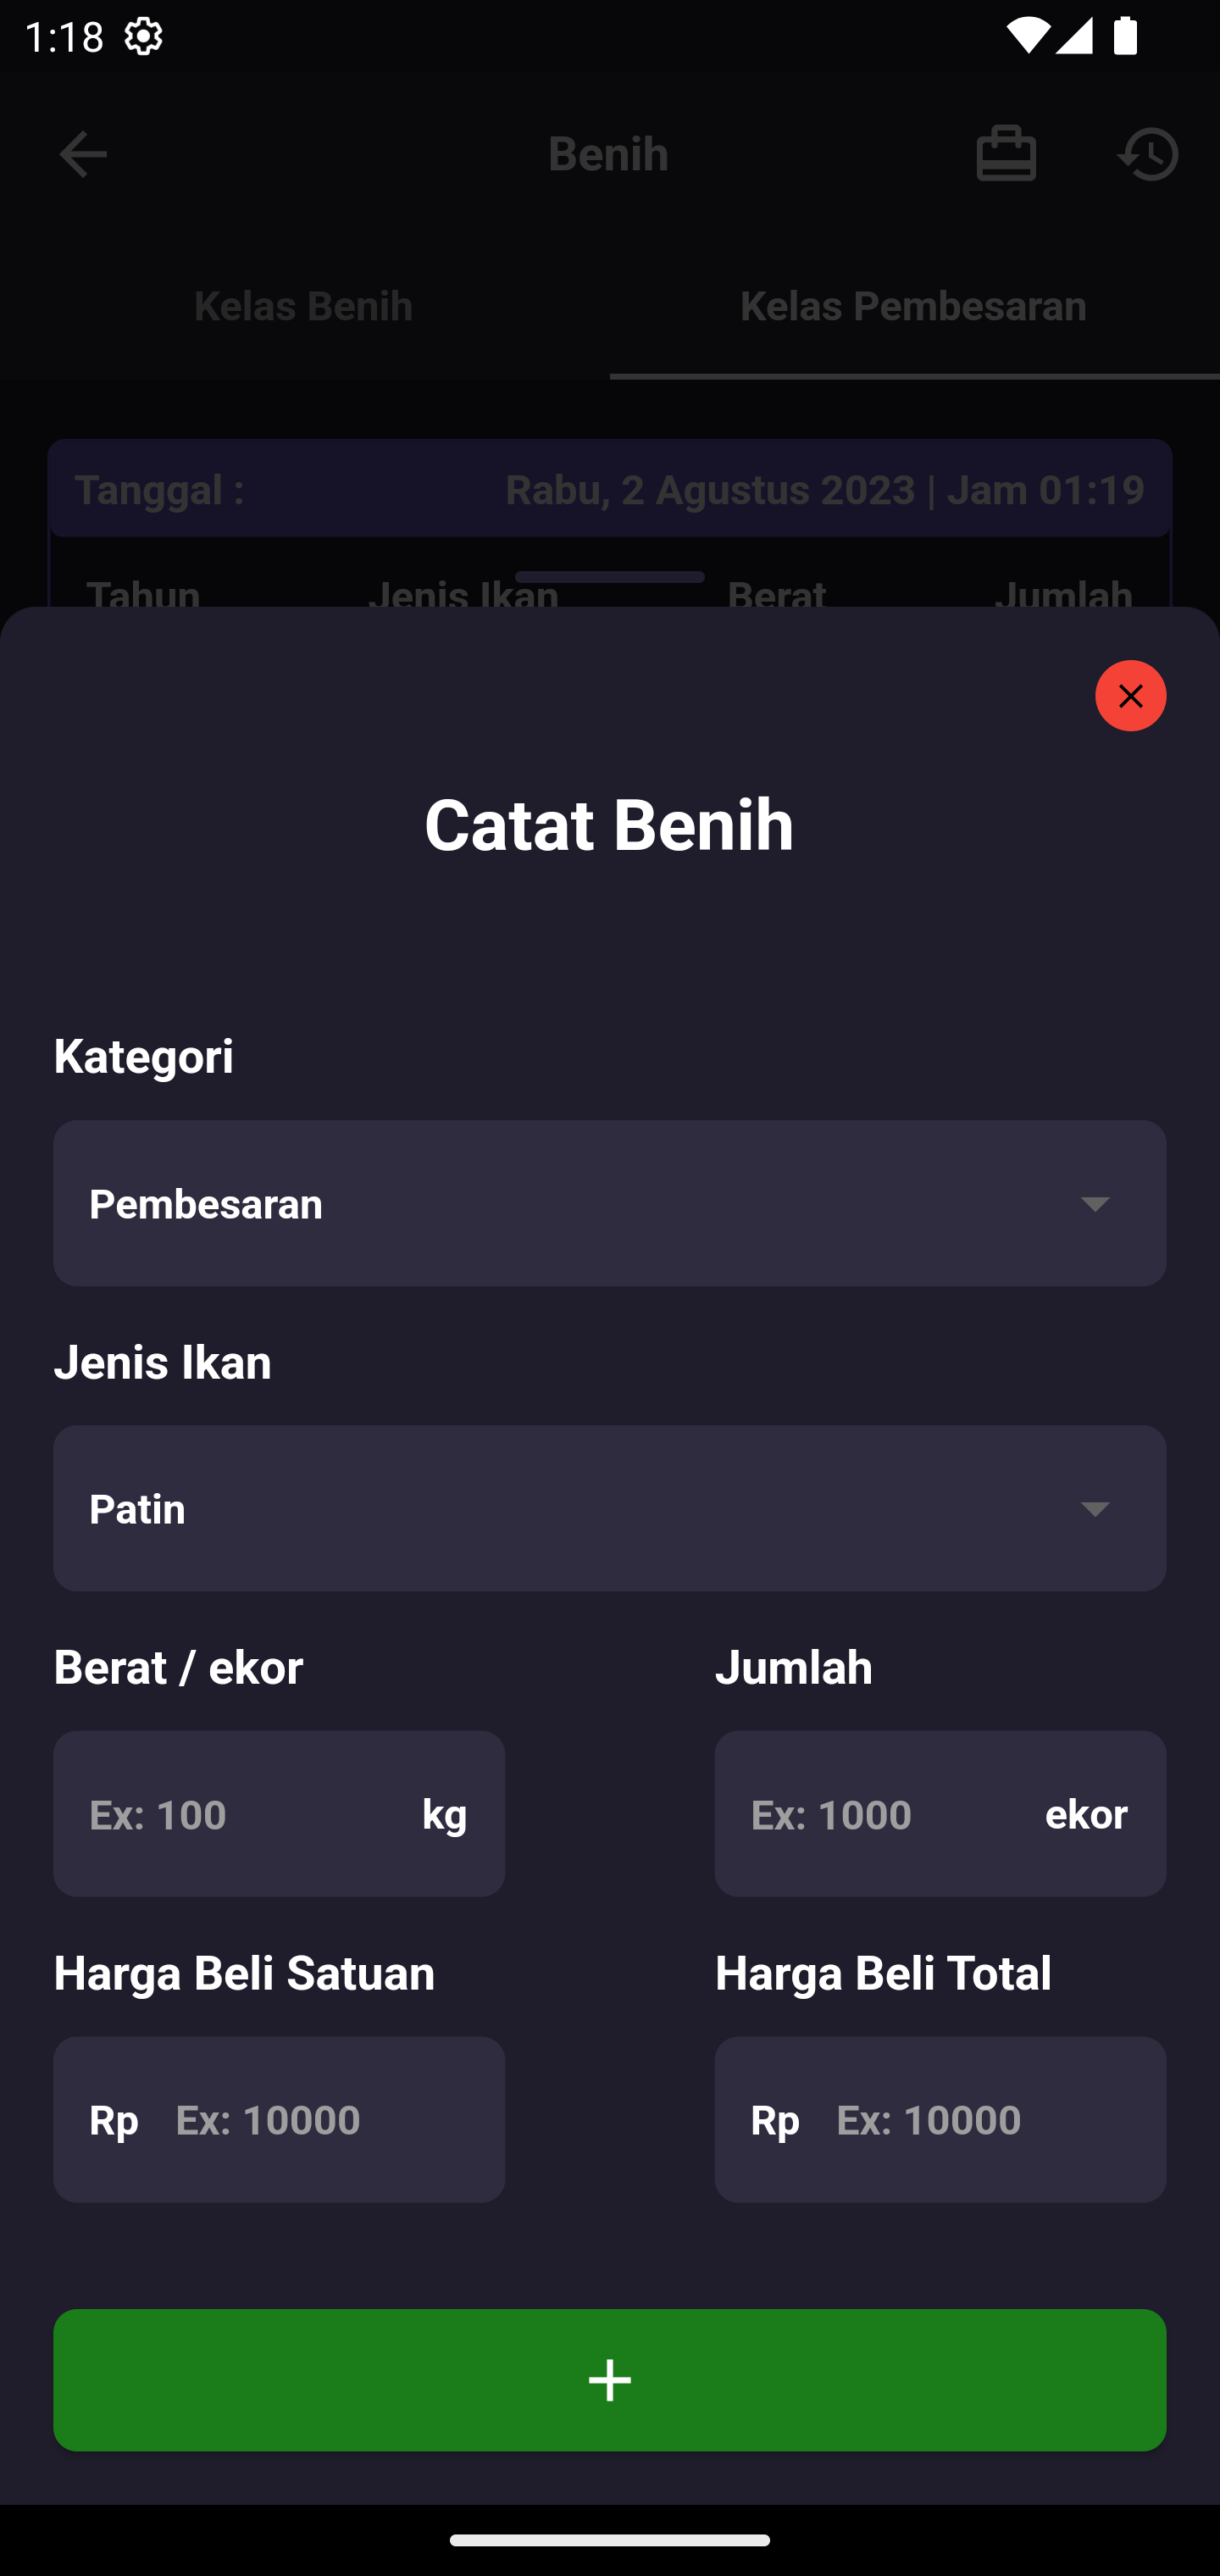
\includegraphics[width=\linewidth]{gambar/sprint3/benih_2.png}
				\caption{Halaman Input Inventaris Benih}
			\endminipage\hfill
			\minipage{0.32\textwidth}
				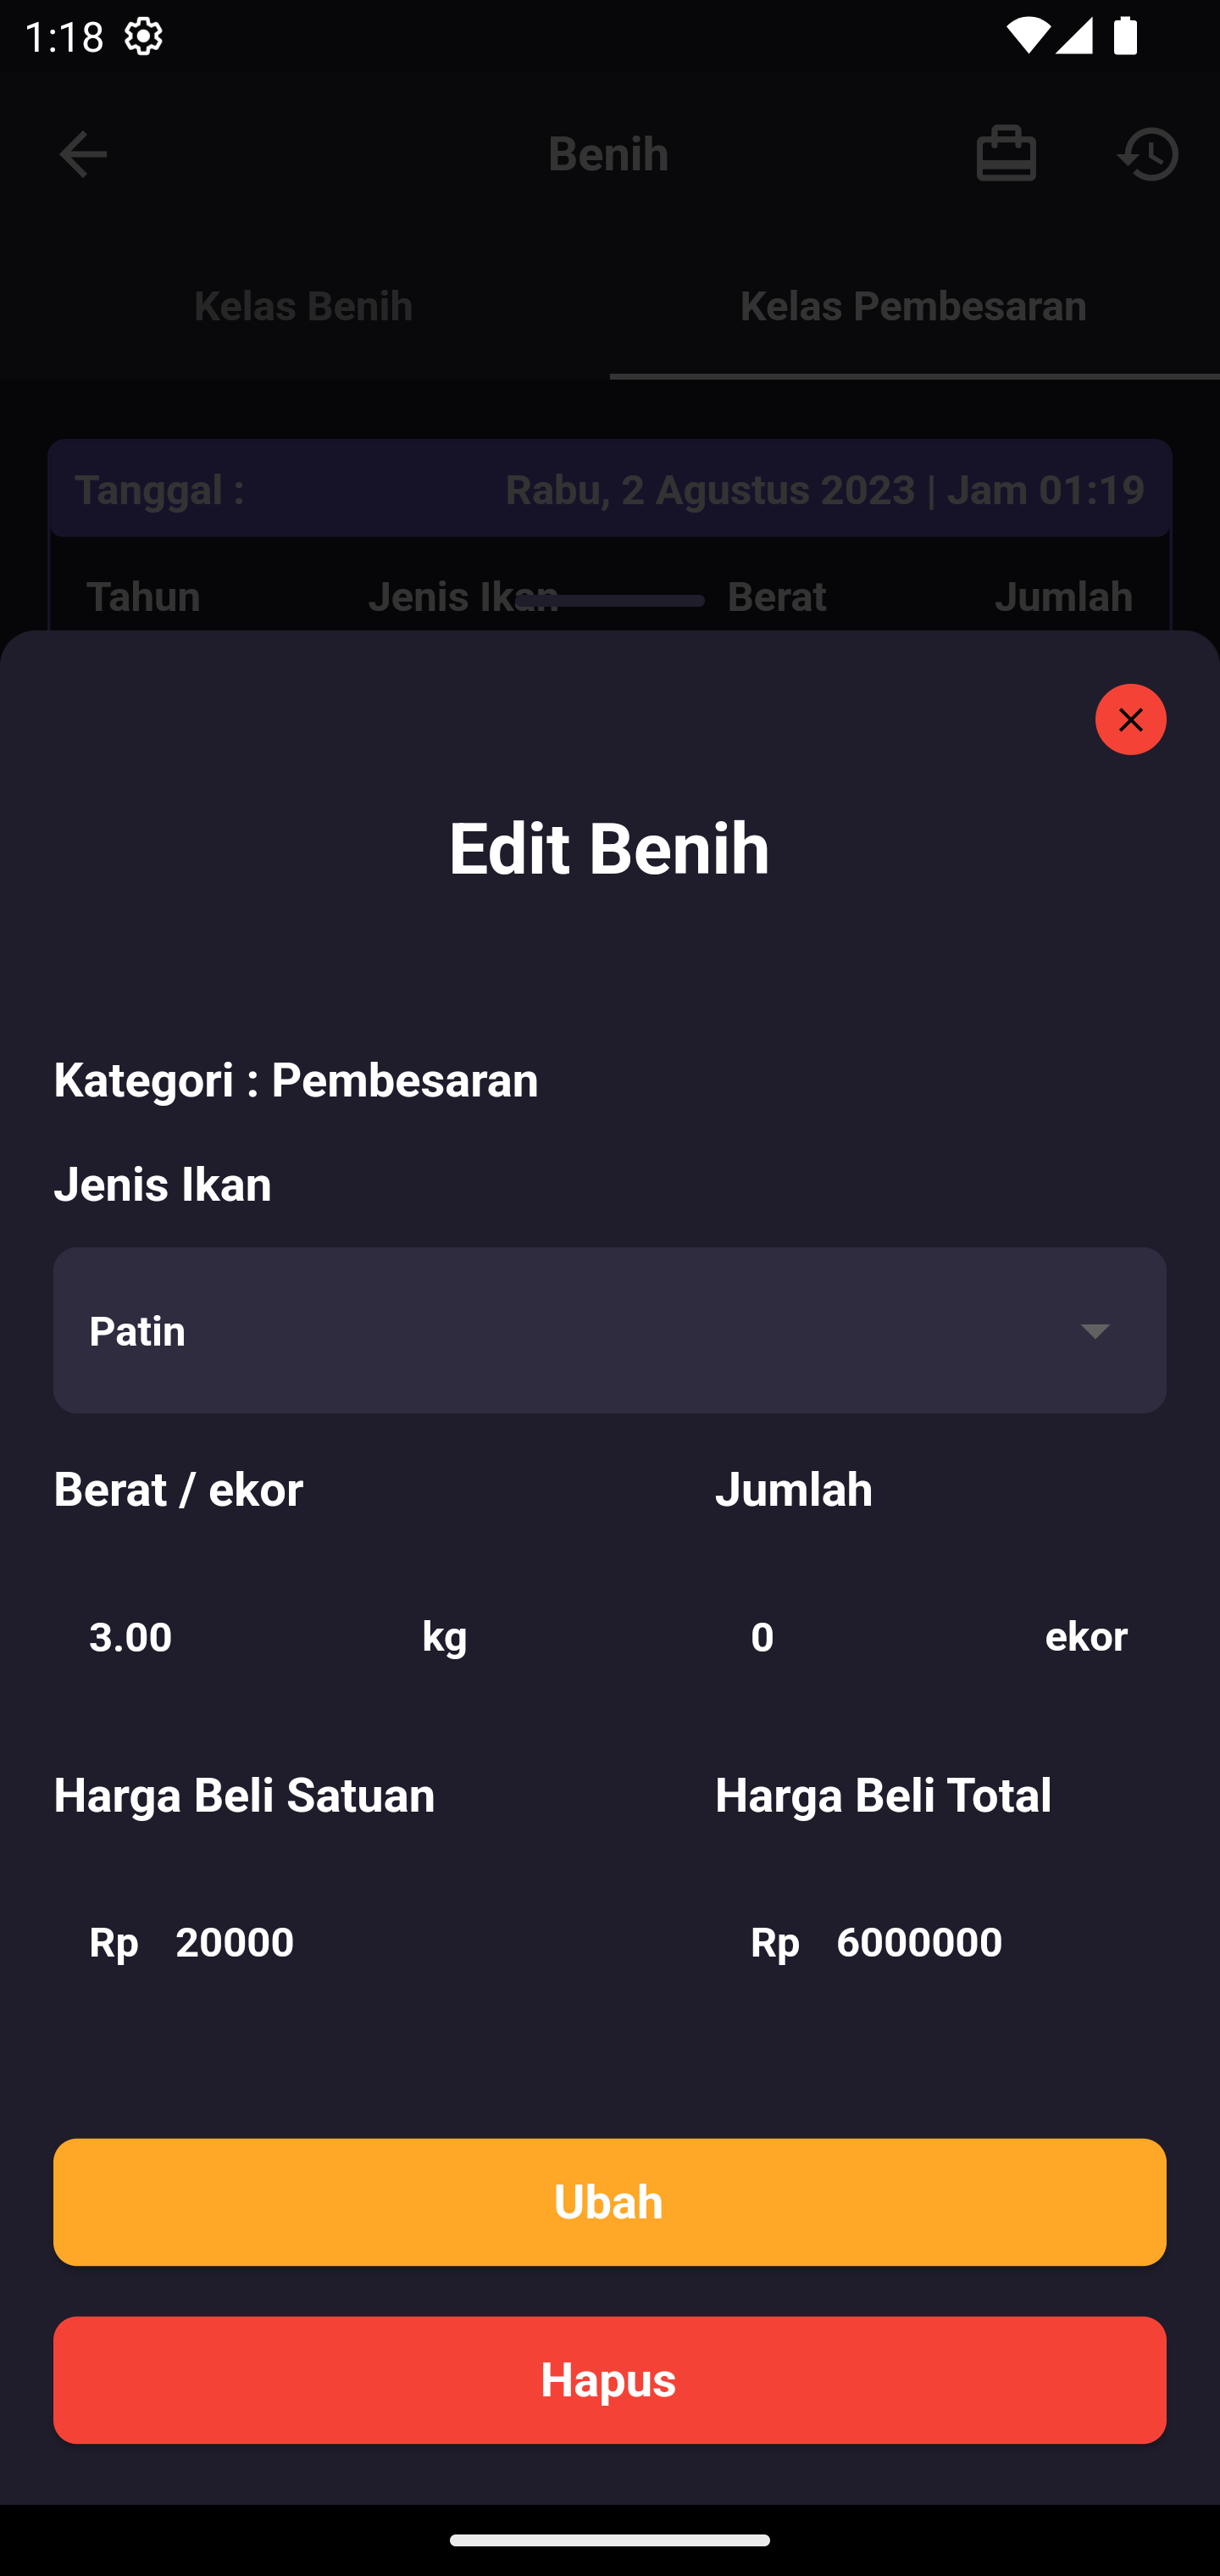
\includegraphics[width=\linewidth]{gambar/sprint3/benih_3.png}
				\caption{Halaman Detail Inventaris Benih}
			\endminipage
		\end{figure}

		\begin{enumerate}
			\item Halaman Inventaris Benih

			Pada halaman ini, terdapat list dari benih yang dibagi menjadi dua kelas yaitu kelas benih dan kelas pembesaran. Pada bagian header layar, terdapat tombol tas untuk menuju ke menu inventaris dan tombol riwayat untuk masuk ke halaman riwayat penggunaan benih.

			Di pojok kanan bawah, terdapat tombol (+) yang berfungsi untuk menavigasikan ke halaman input inventaris benih.

			\item Halaman Input Inventaris Benih
			
			Halaman ini berisi form-form input yang diperlukan untuk pendataan benih.
			
			\item Halaman Detail Inventaris Benih
			
			Halaman ini serupa dengan halaman input inventaris benih, yang membedakan adalah 
			
			Dari tampilan tersebut, bagian yang membedakan dengan halaman input inventaris benih adalah form nya tidak langsung dapat di edit dan terdapat dua tombol tambahan yaitu tombol Edit untuk memperbarui data dan tombol Hapus untuk menghapus data.
		\end{enumerate}

		Untuk inventaris benih digunakan pada saat aktivasi kolam dilakukan. Berikut merupakan tampilan dari aktivasi kolam yang sudah diperbarui dengan data inventaris benih.

		\begin{figure}[H]
			\minipage{0.32\textwidth}
				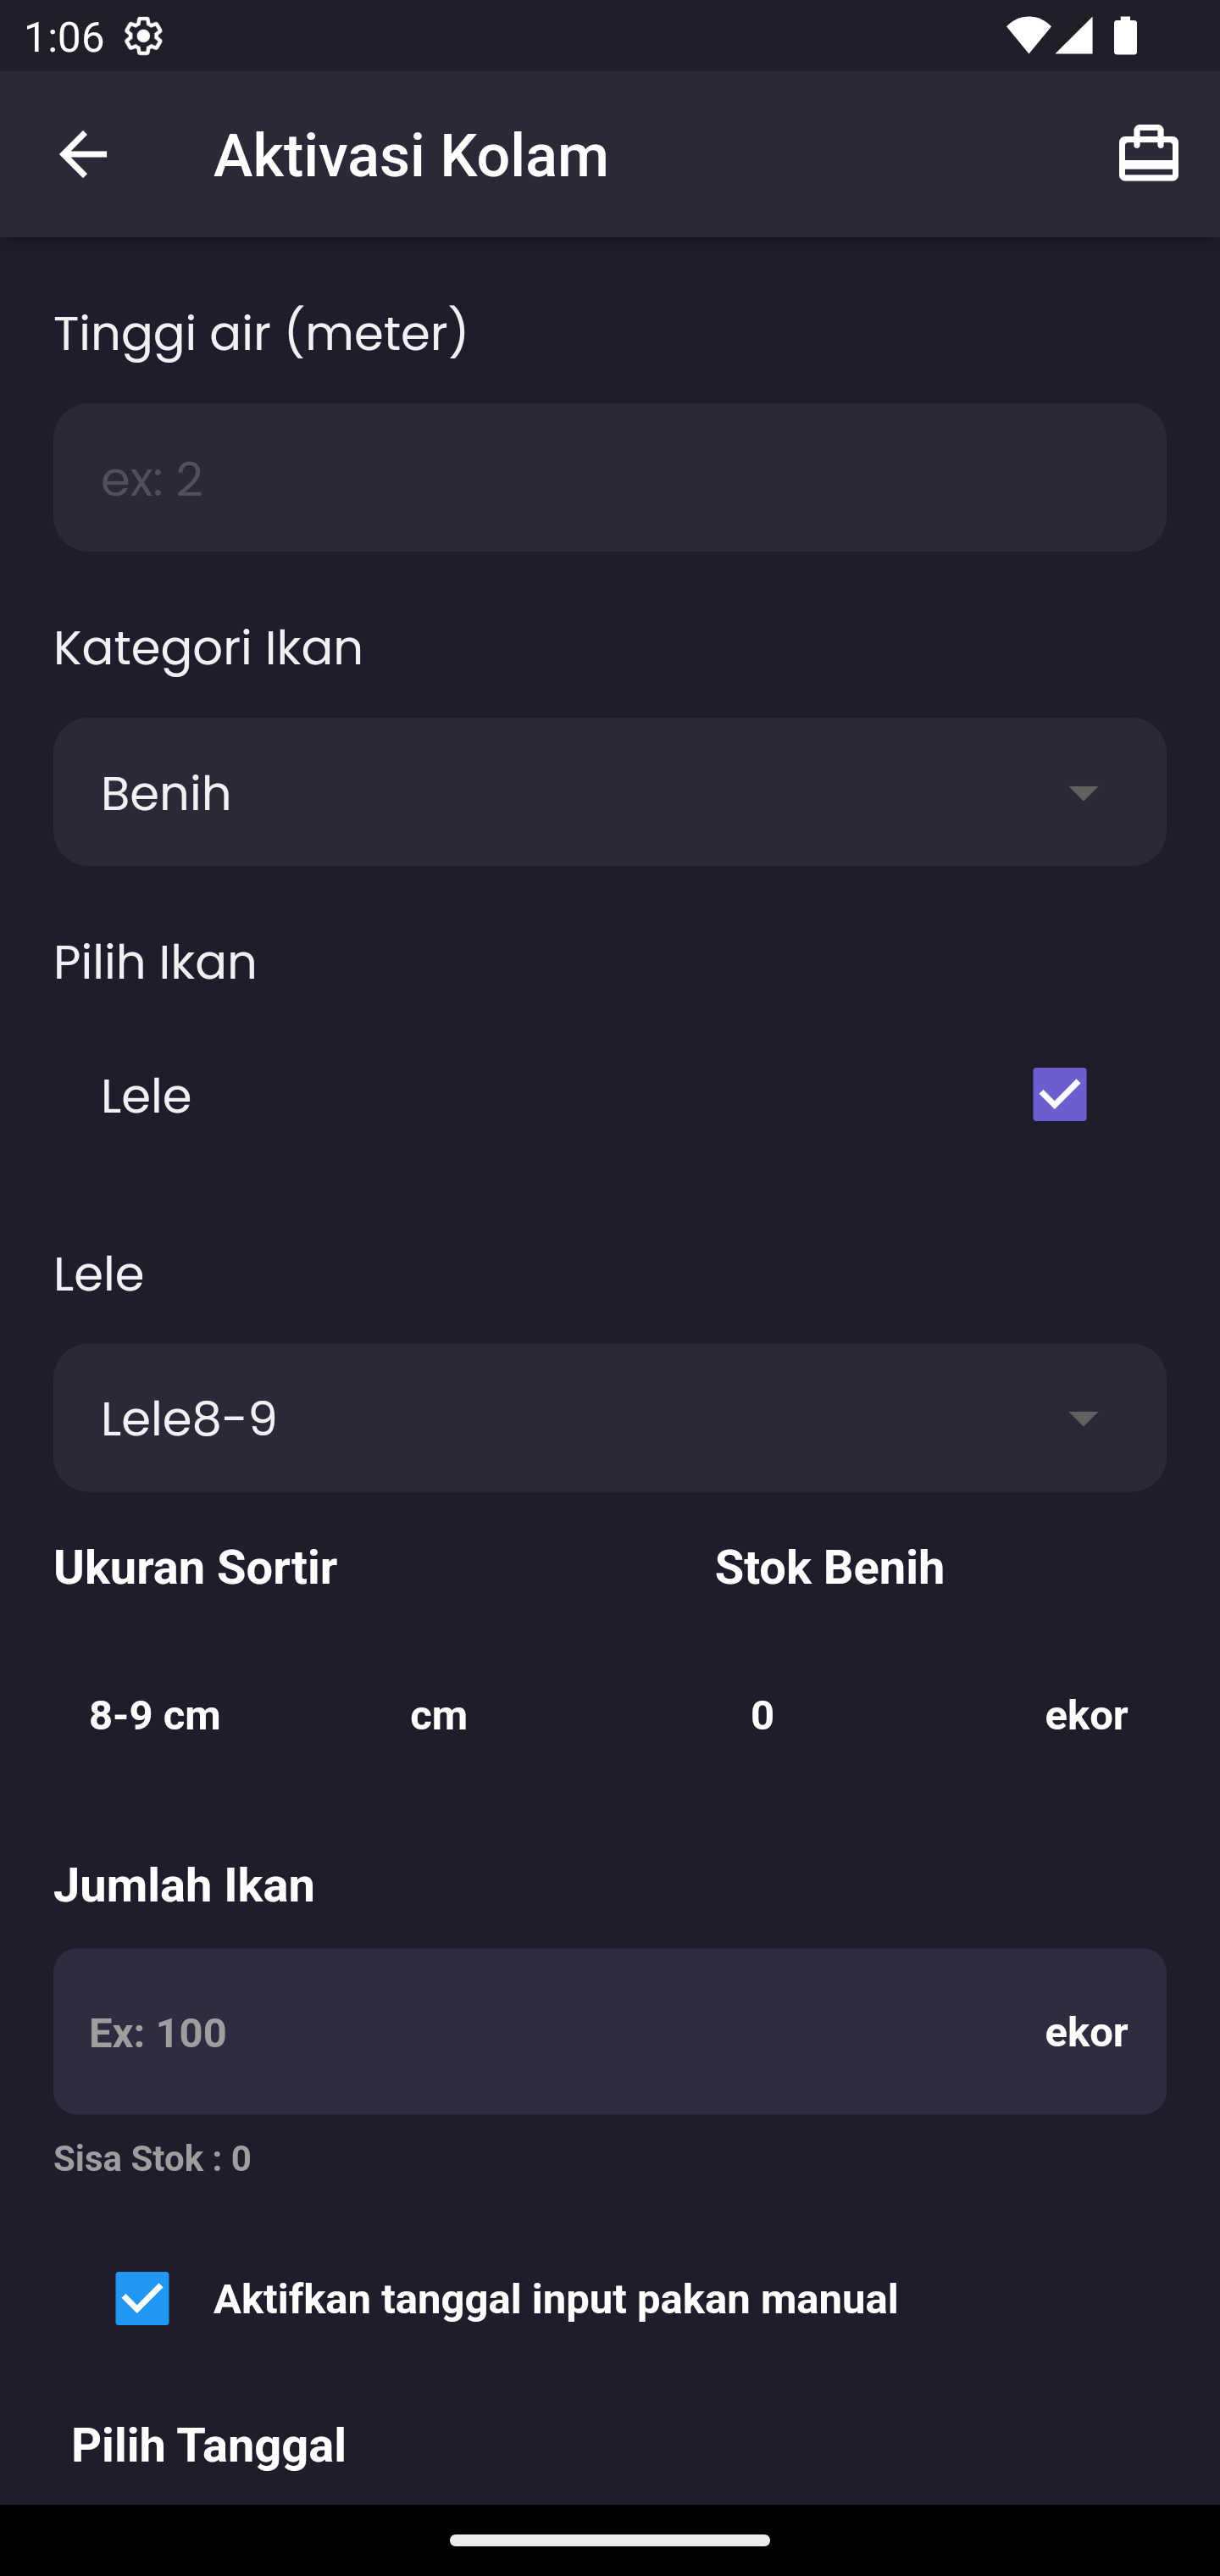
\includegraphics[width=\linewidth]{gambar/sprint4/aktivasi_1.png}
				\caption{Halaman Aktivasi Kolam}
			\endminipage\hfill
			\minipage{0.32\textwidth}
				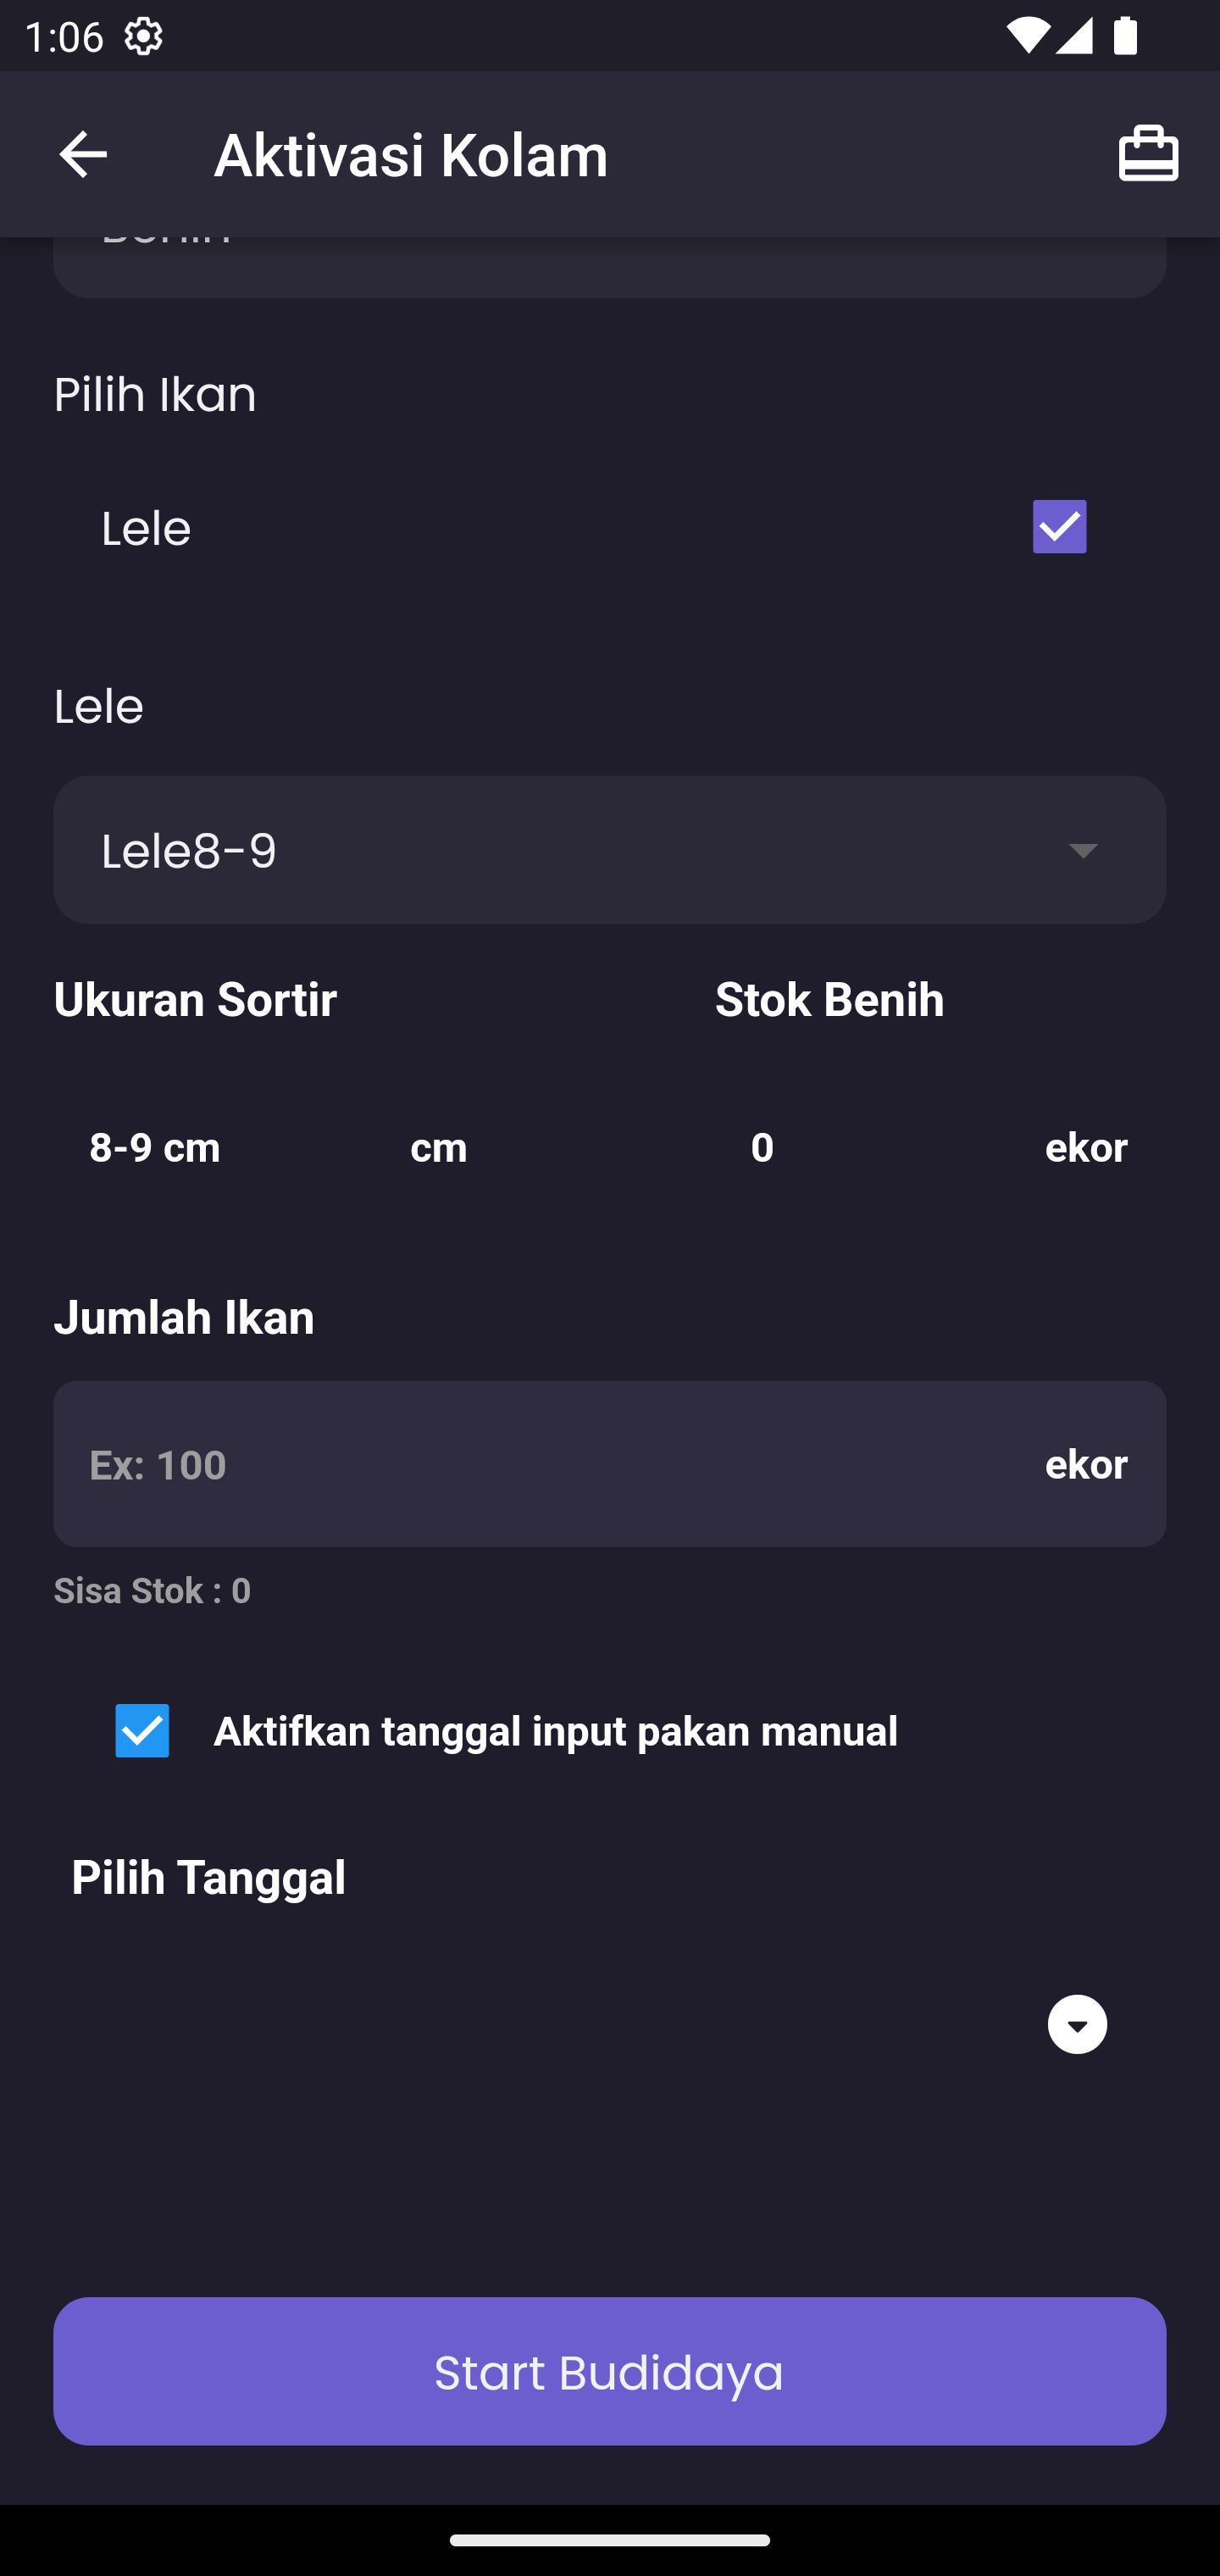
\includegraphics[width=\linewidth]{gambar/sprint4/aktivasi_2.png}
				\caption{Halaman Aktivasi Kolam}
			\endminipage\hfill
		\end{figure}

		Pada halaman tersebut, dapat dilihat benih yang tersedia pada inventaris beserta dengan informasi-informasi mengenai benih tersebut.

		\item Membuat model riwayat pemakaian benih
		
		Dalam penggunaan inventaris benih, diperlukan fitur riwayat penggunaan benih untuk melihat pengeluaran benih ikan tiap musim budidaya. Untuk membuat fitur ini, hal yang pertama dilakukan adalah membuat model dari riwayat pemakaian benih. Model dapat dilihat sebagai berikut.

		\begin{lstlisting}
			class SeedUsed(db.Document):
				fish_seed_id = db.ReferenceField(SeedInventory, required=True)
				farm_id = db.ReferenceField(Farm, required=True)
				original_amount = db.IntField(required=True)
				usage = db.IntField(required=True)
				pond = db.StringField(required=True)
				created_at = db.DateTimeField(default=datetime.datetime.now)
				updated_at = db.DateTimeField(default=datetime.datetime.now)
		\end{lstlisting}

		\item Design route dan penerapan dengan Flutter untuk riwayat pemakaian benih (dalam bentuk RESTful API)
		
		Setelah model selesai, dibuat route yang kemudian diintegrasikan kepada class riwayat benih pada backend.

		\begin{figure}[H]
			\centering
			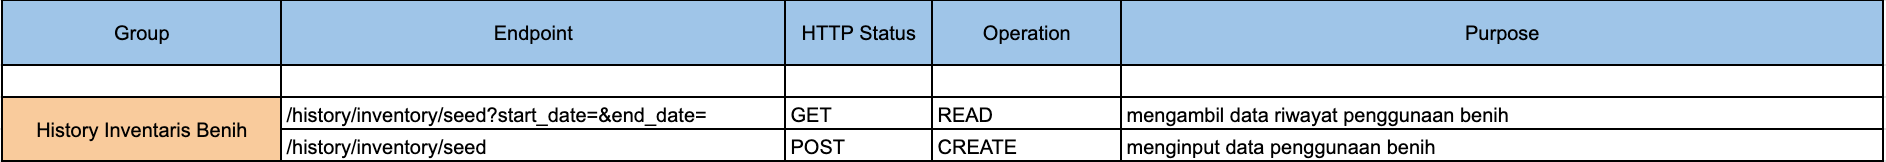
\includegraphics[width=1\textwidth]{gambar/sprint3/history_benih_route.png}
			\caption{Sample Route Riwayat Benih}
		\end{figure}

		\begin{lstlisting}
			api.add_resource(SeedHistoryApi, '/api/history/inventory/seed')
		\end{lstlisting}

		Beberapa fungsi dari class riwayat benih ini dapat dilihat pada kode dibawah ini.

		\begin{enumerate}
			\item Mengambil data riwayat pemakaian benih (HTTP Method - GET) 
			
			\begin{lstlisting}
				class SeedHistoryApi(Resource):
					@jwt_required()

					def get(self):
						try:
				
							current_user = get_jwt_identity()
							farm = str(current_user['farm_id'])
							farm_id = ObjectId(farm)
				
							start_date = datetime.datetime.strptime(request.args.get('start_date'), '%Y-%m-%d') if request.args.get('start_date') else datetime.datetime.strptime("2023-01-01", '%Y-%m-%d')
							end_date = datetime.datetime.strptime(request.args.get('end_date'), '%Y-%m-%d') + datetime.timedelta(days=1) if request.args.get('end_date') else datetime.datetime.strptime("2030-01-01", '%Y-%m-%d')
							name = request.args.get('name') if request.args.get('name') else ""
							pond_name = request.args.get('pond_name') if request.args.get('pond_name') else ""
				
							pipeline = [
								{
									'$match': {
										'created_at': {
											'$gte': start_date,
											'$lte': end_date,
										}
									}
								},
								{
									'$match': {
										"farm_id": farm_id,
										'pond': {
											'$regex': pond_name,
											'$options': 'i'
										}
									}
								},
								{"$sort": {"fish_seed_id": 1}},
								{'$lookup': {
									'from': 'seed_inventory',
									'let': {"fishseedid": "$fish_seed_id"},
									'pipeline': [
										{'$match': {'$expr': {'$eq': ['$_id', '$$fishseedid']}}, },
										{
											'$match': {
												'brand_name': {
													'$regex': name,
													'$options': 'i'
												}
											}
										},
										{"$project": {
											"_id": 1,
											"fish_seed_category": 1,
											"fish_type": 1,
											"brand_name": 1,
											"price": 1,
											"created_at": 1,
										}}
									],
									'as': 'seed'
								}},
								{"$addFields": {
									"seed": {"$first": "$seed"},
								}},
							]
				
							testing = SeedUsed.objects.aggregate(pipeline)
							temp = list(testing)
							result = []
				
							for i in temp:
								if 'seed' in i:
									result.append(i)
							
				
							response = json.dumps({
								'status': 'success',
								'data': result,
							}, default=str)
							return Response(response, mimetype="application/json", status=200)
						except Exception as e:
							response = {"message": e}
							response = json.dumps(response, default=str)
							return Response(response, mimetype="application/json", status=400)
			\end{lstlisting}

			Pada fungsi tersebut, terdapat empat query params yang berguna untuk memfilter data yaitu start\_date yang bernilai tanggal awal, end\_date yang bernilai tanggal akhir, name yang bernilai nama benih, dan pond\_name yang bernilai nama kolam.

			Untuk response data riwayat benih, disini dilakukan \$lookup pada pipeline untuk mengambil data pada database inventaris benih untuk menampilkan detail data benih.

			\item Membuat data riwayat pemakaian benih (HTTP Method - POST)
			
			\begin{lstlisting}
				class SeedHistoryApi(Resource):
					@jwt_required()
					def post(self):
						try:
							current_user = get_jwt_identity()
							farm = str(current_user['farm_id'])
						
							req_pond = request.form.get('pond', None)
							req_seed_id = request.form.get('fish_seed_id', None)
							req_usage = request.form.get('usage', None) 
							
							history_by_pond =  SeedUsed.objects(pond=req_pond, fish_seed_id=req_seed_id).first()
				
							print(history_by_pond)
				
							theDate = request.form.get('created_at', None)
				
							body = {
								"farm_id": farm,
								"fish_seed_id": request.form.get('fish_seed_id', None),
								"original_amount": request.form.get('original_amount', None),
								"usage": request.form.get('usage', None),
								"pond": request.form.get('pond', None),
							}
				
							if theDate != '':
								body['created_at'] = datetime.datetime.strptime(theDate, "%Y-%m-%dT%H:%M:%S.%f %z") 
								
						except Exception as e:
							response = {"message": str(e)}
							response = json.dumps(response, default=str)
							return Response(response, mimetype="application/json", status=400)
			\end{lstlisting}
		\end{enumerate}

		Setelah fungsi selesai, dibuat controller riwayat benih pada Flutter yang berisi fungsi yang sesuai pada class riwayat benih.

		\begin{enumerate}
			\item Mengambil data riwayat pemakaian benih (HTTP Method - GET) 
			
			\begin{lstlisting}
				Future getHistorySeedData(bool isReversed, String firstDate, String lastDate,
					String name, Function() doAfter) async {
						seedHistoryList.value.data!.clear();
						isLoadingHistory.value = true;
					
						SharedPreferences prefs = await SharedPreferences.getInstance();
						String token = prefs.getString('token').toString();
						var headers = {'Authorization': 'Bearer $token'};
					
						final response = await http.get(
							Uri.parse(
								'${Urls.seedSch}?start_date=$firstDate&end_date=$lastDate&name=$name'),
							headers: headers,
						);
					
						try {
							if (response.statusCode == 200) {
							HistorySeedModel res =
								HistorySeedModel.fromJson(jsonDecode(response.body));
					
							if (isReversed) {
								var temp = res;
								seedHistoryList.value.data = temp.data!.reversed.toList();
							} else {
								var temp = res;
								seedHistoryList.value.data = temp.data!;
							}
					
							doAfter();
							}
						} catch (e) {
							throw Exception(e);
						}
						isLoadingHistory.value = false;
					}
			\end{lstlisting}

			\item Membuat data riwayat pemakaian benih (HTTP Method - POST)
			
			\begin{lstlisting}
				Future postHistorySeedData(
					String pondName, List fish, String usedDate, Function() doAfter) async {
					var map = <String, dynamic>{};

					map['pond'] = pondName;

					SharedPreferences prefs = await SharedPreferences.getInstance();
					String token = prefs.getString('token').toString();
					var headers = {'Authorization': 'Bearer $token'};

					for (var i = 0; i < fish.length; i++) {
						map['fish_seed_id'] = fish[i]['seed_id'];
						map['original_amount'] = fish[i]['original_value'];
						map['usage'] = fish[i]['amount'];
						map['created_at'] = usedDate;

						try {
							await http.post(
							Uri.parse(Urls.seedSch),
							body: map,
							headers: headers,
							);
							doAfter();
						} catch (e) {
							throw Exception(e);
						}
					}
				}
			\end{lstlisting}
		\end{enumerate}

		Setelah controller sudah siap digunakan, untuk tampilan dari riwayat pemakaian benih dapat dilihat pada layout dan code berikut.

		\begin{figure}[H]
			\centering
			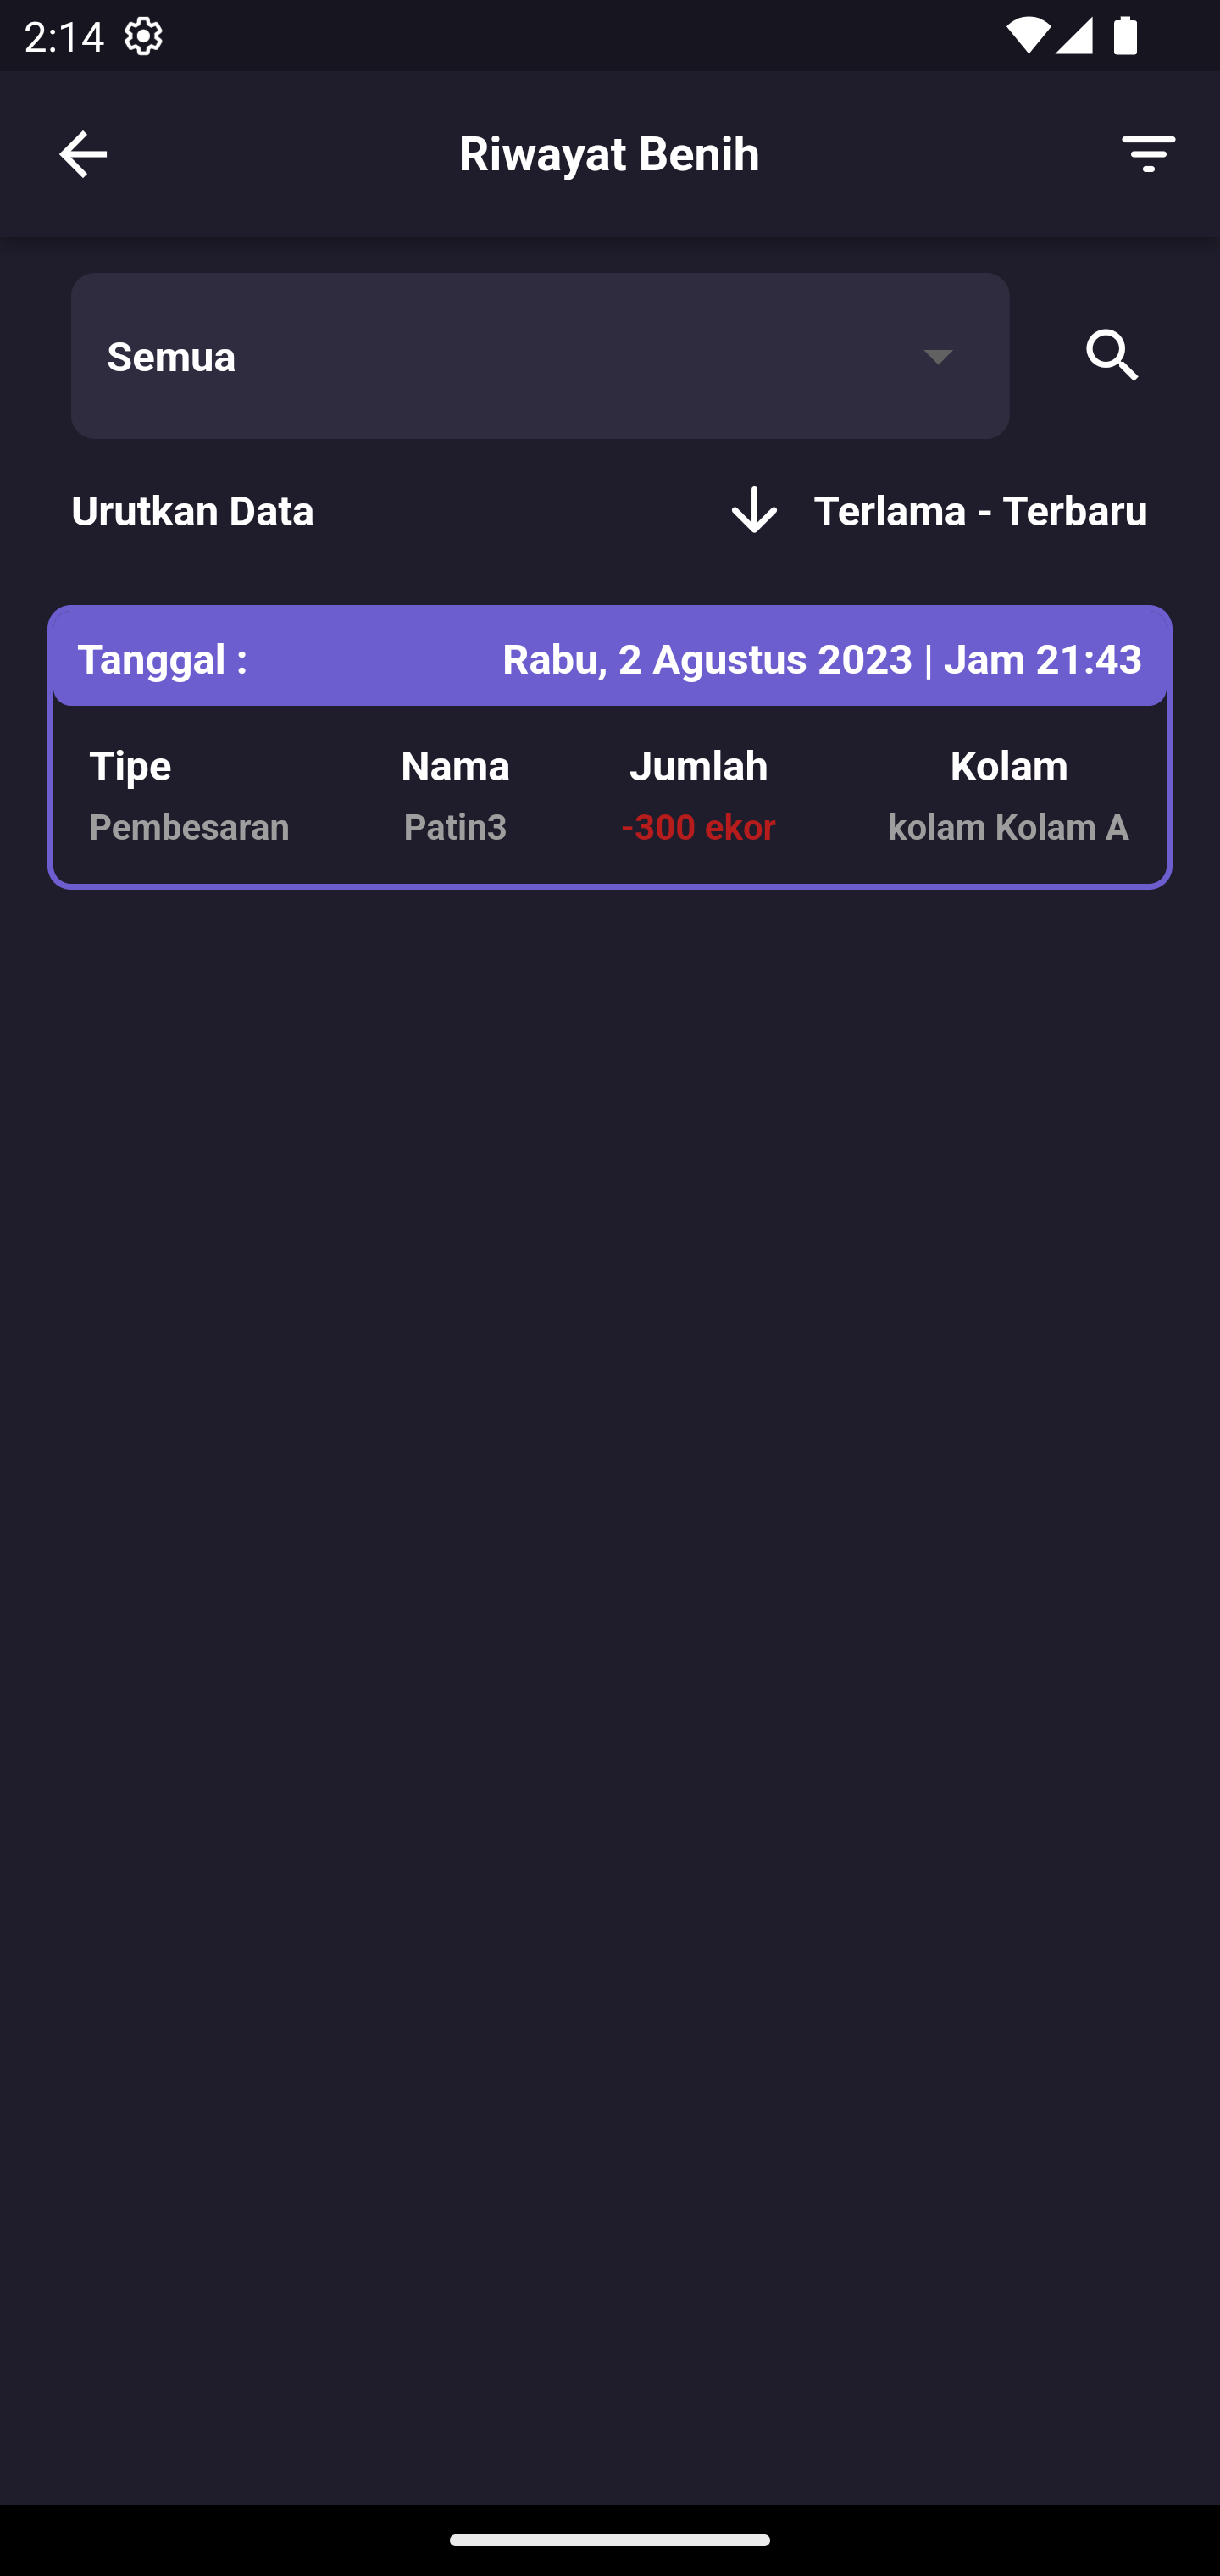
\includegraphics[width=0.3\textwidth]{gambar/sprint3/detail_benih.png}
			\caption{Halaman Penggunaan Benih}
		\end{figure}

		Pada halaman tersebut, terdapat list dari penggunaan benih. Rincian data yang ditampilkan adalah tipe, nama, jumlah, dan tempat kolam benih diletakkan. Terdapat juga beberapa layout yang digunakan untuk memfilter data.

		\item Sprint 3 Review
		
		Hasil review pada Sprint 3 ini adalah review dan testing oleh penulis selaku developer dengan Scrum Master. Setelah dilakukan testing, Scrum Master menyimpulkan bahwa penerapan fitur inventaris benih dan riwayat benih telah berjalan dengan baik.
 
	\end{enumerate}

\subsection{Sprint 4}

	Sprint 4 dilaksanakan pada tanggal 21 Juni 2023 - 12 Juli 2023. Detail dari Sprint 4 ini adalah mengerjakan tugas yang ada pada Sprint 4 Backlog di tabel berikut.
	
	\begin{table}[H]	
		\begin{center}
			\caption{Sprint 4 Backlog}
			\label{tab:table21}
			\begin{tabular}{|c|c|m{13em}|c|}
			\hline
			\textbf{No} & \textbf{Stories} & \textbf{Task} & \textbf{Status} \\
			\hline
			1 & \multirow{1}{12em}{Fitur pencatatan inventaris} & - Design route dan penerapan pada Flutter untuk inventaris pakan (dalam bentuk RESTful API) & Selesai \\
			\hline
			&  & - Design route dan penerapan pada Flutter untuk inventaris suplemen (dalam bentuk RESTful API) & Selesai  \\ 
			\hline
			&  & - Design route dan penerapan pada Flutter untuk inventaris listrik (dalam bentuk RESTful API) & Selesai  \\ 
			\hline
			&  & - Design route dan penerapan pada Flutter untuk inventaris aset (dalam bentuk RESTful API) & Selesai  \\ 
			\hline
			&  & - Design route dan penerapan pada Flutter untuk riwayat pemakaian pakan (dalam bentuk RESTful API) & Selesai  \\ 
			\hline
			&  & - Design route dan penerapan pada Flutter untuk riwayat pemakaian suplemen (dalam bentuk RESTful API) & Selesai  \\ 
			\hline
			2 & \multirow{1}{12em}{Fitur Pemberian pakan yang terkoneksi dengan inventaris} & - Integrasi data inventaris pakan pada halaman entry pakan  & Selesai \\
			&  &  &  \\ 
			\hline
			\end{tabular}
		\end{center}
	\end{table}


	% \begin{table}[H]	
	% 	\begin{center}
	% 		\begin{tabular}{|c|c|m{13em}|c|}
	% 		\hline
	% 		\textbf{No} & \textbf{Stories} & \textbf{Task} & \textbf{Status} \\
	% 		\hline
	% 		&  & - Design route dan penerapan pada Flutter untuk riwayat pemakaian pakan (dalam bentuk RESTful API) & Selesai  \\ 
	% 		\hline
	% 		&  & - Design route dan penerapan pada Flutter untuk riwayat pemakaian suplemen (dalam bentuk RESTful API) & Selesai  \\ 
	% 		\hline
	% 		2 & \multirow{1}{12em}{Fitur Pemberian pakan yang terkoneksi dengan inventaris} & - Integrasi data inventaris pakan pada halaman entry pakan  & Selesai \\
	% 		&  &  &  \\ 
	% 		\hline
	% 		\end{tabular}
	% 	\end{center}
	% \end{table}

	Dalam proses Sprint ini, beberapa tahapan yang dilakukan adalah sebagai berikut :

	\begin{enumerate}
		\item Design route dan penerapan pada Flutter untuk inventaris pakan (dalam bentuk RESTful API)
		
		Untuk melakukan tugas ini, langkah-langkahnya sama seperti yang ada pada Sprint 3. Langkah-langkah yang dilakukan adalah sebagai berikut:

		\begin{enumerate}
			\item Design Sample Route
			
			Berikut merupakan sample route yang sudah dibuat untuk inventaris pakan.

			\begin{figure}[H]
				\centering
				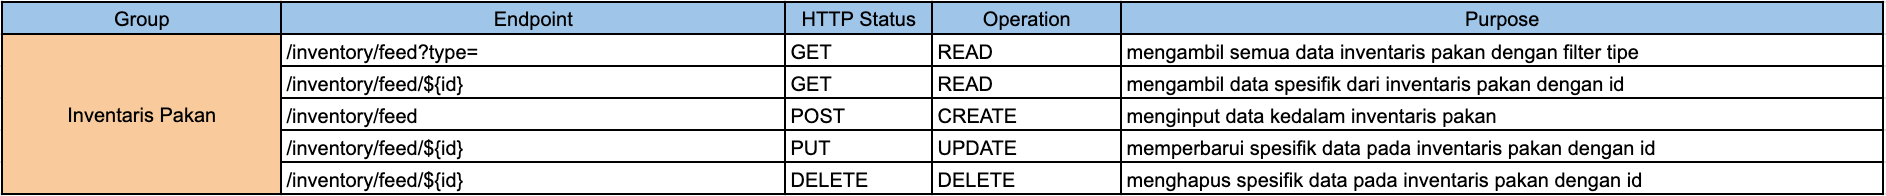
\includegraphics[width=1\textwidth]{gambar/sprint4/sample_route_pakan.png}
				\caption{Sample Route Inventaris Pakan}
			\end{figure}

			\item Model Backend
 			
			Berdasarkan sample route tersebut, dapat dibuat model dan class HTTP method pada backend. Berikut model serta class untuk inventaris pakan :

			\begin{lstlisting}
				class FeedInventory(db.Document):
					feed_name_id = db.ReferenceField(FeedName, required=True)
					farm_id = db.ReferenceField(Farm, required=True)
					id_int = db.SequenceField(required=True)
					feed_category = db.StringField(required=True)
					brand_name = db.StringField(required=True)
					price = db.IntField(required=True)
					amount = db.FloatField(required=True)
					created_at = db.DateTimeField(default=datetime.datetime.now)
					updated_at = db.DateTimeField(default=datetime.datetime.now)	
			\end{lstlisting}

				% Pada model tersebut, terdapat beberapa \textit{key} seperti feed\_name\_id yang digunakan untuk mereferensikan kepada tabel FeedName, farm\_id untuk mereferensikan kepada tabel Farm, id\_int untuk 
				% Pada model ini, \dots

	
			\item Fungsi-fungsi HTTP Method
			
			\begin{itemize}
				\item Mengambil semua data inventaris pakan (HTTP Method - GET)
				
				\begin{lstlisting}
					class FeedInventoriesApi(Resource):
						@jwt_required()

						def get(self):
							try:
								current_user = get_jwt_identity()
								farm = str(current_user['farm_id'])
								farm_id = ObjectId(farm)
					
								type = request.args.get('type') if request.args.get('type') else ""
					
								pipeline = [
									{"$sort": {"id_int": 1}},
									{
										'$match': {
											"farm_id": farm_id,
											'feed_category': {
												'$regex': type,
												'$options': 'i'
											}
										}
									},
									{'$lookup': {
										'from': 'feed_name',
										'let': {"feednameid": "$feed_name_id"},
										'pipeline': [
											{'$match': {'$expr': {'$eq': ['$_id', '$$feednameid']}}},
											{"$project": {
												"_id": 1,
												"id_int": 1,
												"type": 1,
												"name": 1,
												"description": 1,
												"producer": 1,
												"protein": 1,
												"carbohydrate": 1,
												"min_expired_period": 1,
												"max_expired_period": 1,
												"image": 1,
												"created_at": 1,
											}}
										],
										'as': 'feed'
									}},
									{"$addFields": {
										"feed": {"$first": "$feed"},
									}},
								]
							
								testing = FeedInventory.objects.aggregate(pipeline)
								temp = list(testing)
								response = json.dumps({
									'status': 'success',
									'data': temp,
								}, default=str)
								return Response(response, mimetype="application/json", status=200)
							except Exception as e:
								response = {"message": e}
								response = json.dumps(response, default=str)
								return Response(response, mimetype="application/json", status=400)
				\end{lstlisting}

				\item Mengambil spesifik data inventaris pakan (HTTP Method - GET)
				
				\begin{lstlisting}
					class FeedInventoryApi(Resource):
						def get(self, id):
							try:
								pipeline = [
									{"$match": {"id_int": int(id)}},
									{'$lookup': {
										'from': 'feed_name',
										'let': {"feednameid": "$feed_name_id"},
										'pipeline': [
											{'$match': {'$expr': {'$eq': ['$_id', '$$feednameid']}}},
											{"$project": {
												"_id": 1,
												"id_int": 1,
												"type": 1,
												"name": 1,
												"description": 1,
												"producer": 1,
												"protein": 1,
												"carbohydrate": 1,
												"min_expired_period": 1,
												"max_expired_period": 1,
												"image": 1,
												"created_at": 1,
											}}
										],
										'as': 'feed'
									}},
									{"$addFields": {
										"feed": {"$first": "$feed"},
									}},
								]
						
								testing = FeedInventory.objects.aggregate(pipeline)
								temp = list(testing)
								if len(temp) == 0:
									res = {"message": 'no data found'}
									response = json.dumps(res, default=str)
									return Response(response, mimetype="application/json", status=200)
								response = json.dumps({
									'status': 'success',
									'data': temp[0],
								}, default=str)
								return Response(response, mimetype="application/json", status=200)
							except Exception as e:
								response = {"message": e}
								response = json.dumps(response, default=str)
								return Response(response, mimetype="application/json", status=400)
				\end{lstlisting}

				\item Menambahkan data inventaris pakan (HTTP Method - POST)
				
				\begin{lstlisting}
					class FeedInventoriesApi(Resource):
						@jwt_required()
						def post(self):
							try:
								current_user = get_jwt_identity()
								farm = str(current_user['farm_id'])
								body = {
									"feed_name_id": request.form.get('feed_name_id', None),
									"feed_category": request.form.get('feed_category', None),
									"brand_name": request.form.get('brand_name', None),
									"price": request.form.get('price', None),
									"amount": request.form.get('amount', None),
								}
								inventory = FeedInventory(**body).save()
								id = inventory.id
								res = {"message": "success add feed to inventory", "id": id, "data": body}
								response = json.dumps(res, default=str)
								return Response(response, mimetype="application/json", status=200)
							except Exception as e:
								response = {"message": str(e)}
								response = json.dumps(response, default=str)
								return Response(response, mimetype="application/json", status=400)
				\end{lstlisting}

				\item Memperbarui spesifik data inventaris pakan (HTTP Method - PUT)
				
				\begin{lstlisting}
					class FeedInventoryApi(Resource):
						def put(self, id):
							try:
								body = {
									"id_int": int(id),		
									"feed_category": request.form.get('feed_category', None),
									"brand_name": request.form.get('brand_name', None),
									"price": request.form.get('price', None),
									"amount": request.form.get('amount', None),
								}

								feed_name_id = request.form.get('feed_name_id', None)
								feed_name = FeedName.objects.get(id=feed_name_id)
								body["feed_name_id"] = feed_name.id

								inventory = FeedInventory.objects.get(id_int = int(id)).update(**body)
								response = {"message": "success update feed inventory", "data": body}
								response = json.dumps(response, default=str)
								return Response(response, mimetype="application/json", status=200)
							except Exception as e:
								response = {"message": str(e)}
								response = json.dumps(response, default=str)
								return Response(response, mimetype="application/json", status=400)
				\end{lstlisting}

				\item Menghapus spesifik data inventaris pakan (HTTP Method - DELETE)
				
				\begin{lstlisting}
					class FeedInventoryApi(Resource):
						def delete(self, id):
							try:
								inventory = FeedInventory.objects.get(id_int = int(id)).delete()
								response = {"message": "success delete feed inventory"}
								response = json.dumps(response, default=str)
								return Response(response, mimetype="application/json", status=200)
							except Exception as e:
								response = {"message": str(e)}
								response = json.dumps(response, default=str)
								return Response(response, mimetype="application/json", status=400)
				\end{lstlisting}
			\end{itemize}

			\item Controller HTTP pada Flutter
			
			\begin{itemize}
				\item Mengambil semua data inventaris pakan (HTTP Method - GET)
				
				\begin{lstlisting}
					Future getAllData(String type, Function() doAfter) async {
						feedList.value.data!.clear();
						selectedFeedList.clear();
						isLoadingPage.value = true;

						SharedPreferences prefs = await SharedPreferences.getInstance();
						String token = prefs.getString('token').toString();
						var headers = {'Authorization': 'Bearer $token'};

						final response = await http.get(
						Uri.parse('${Urls.invFeed}?type=$type'),
						headers: headers,
						);

						try {
						if (response.statusCode == 200) {
							InventarisPakanModel res =
								InventarisPakanModel.fromJson(jsonDecode(response.body));

							feedList.value = res;

							for (var i in feedList.value.data!) {
							selectedFeedList.add({
								'id': i.idInt,
								'feed_id': i.sId,
								'feed_name': i.brandName,
							});

							selectedFeedName.value = selectedFeedList[0];
							}

							inspect(feedList.value.data);

							doAfter();
						}
						} catch (e) {
						throw Exception(e);
						}
						isLoadingPage.value = false;
					}
				\end{lstlisting}

				\item Mengambil spesifik data inventaris pakan (HTTP Method - GET)
				
				\begin{lstlisting}
					Future getDataByID(int id, Function() doAfter) async {
						// resetVariables();
						isLoadingDetail.value = true;
						isLoadingFeedDetail.value = true;
					
						final response = await http.get(Uri.parse('${Urls.invFeed}/$id'));
					
						try {
						  if (response.statusCode == 200) {
							DetailInventarisPakanModel res =
								DetailInventarisPakanModel.fromJson(jsonDecode(response.body));
					
							feedCategory.value = res.data!.feedCategory!;
					
							for (var i in listPakanName) {
							  if (i['feed_name_id'] == res.data!.feedNameId) {
								selectedPakan.value = i;
							  }
							}
					
							// desc.text = res.data!.description.toString();
							price.text = res.data!.price.toString();
							amount.text = res.data!.amount!.toStringAsFixed(2);
							producer.text = res.data!.feed!.producer.toString();
							protein.text = res.data!.feed!.protein.toString();
							carbo.text = res.data!.feed!.carbohydrate.toString();
							minExp.text = res.data!.feed!.minExpiredPeriod.toString();
							// maxExp.text = res.data!.maxExpiredPeriod.toString();
							// image.value = res.data!.image.toString();
						  }
						  doAfter();
						} catch (e) {
						  throw Exception(e);
						}
						isLoadingDetail.value = false;
						isLoadingFeedDetail.value = false;
					  }
				\end{lstlisting}

				\item Menambahkan data inventaris pakan (HTTP Method - POST)
				
				\begin{lstlisting}
					Future postData(Function() doAfter) async {
						var map = <String, dynamic>{};

						map['feed_name_id'] = selectedPakan.value['feed_name_id'];
						map['feed_category'] = feedCategory.value;
						map['brand_name'] = selectedPakan.value['feed_name'];
						map['price'] = price.text;
						map['amount'] = amount.text.replaceAll(',', '.');

						SharedPreferences prefs = await SharedPreferences.getInstance();
						String token = prefs.getString('token').toString();
						var headers = {'Authorization': 'Bearer $token'};

						isLoadingPost.value = true;

						inspect(map);

						try {
						await http.post(
							Uri.parse(Urls.invFeed),
							body: map,
							headers: headers,
						);
						doAfter();
						} catch (e) {
						throw Exception(e);
						}
						isLoadingPost.value = false;
					}
				\end{lstlisting}

				\item Memperbarui spesifik data inventaris pakan (HTTP Method - PUT)
				
				\begin{lstlisting}
					Future updateData(int id, Function() doAfter) async {
						var map = <String, dynamic>{};

						map['feed_name_id'] = selectedPakan.value['feed_name_id'];
						map['feed_category'] = feedCategory.value;
						map['brand_name'] = selectedPakan.value['feed_name'];
						map['price'] = price.text;
						map['amount'] = amount.text.replaceAll(',', '.');

						isLoadingPost.value = true;

						try {
						inspect(map);
						await http.put(
							Uri.parse('${Urls.invFeed}/$id'),
							body: map,
						);
						doAfter();
						} catch (e) {
						throw Exception(e);
						}
						isLoadingPost.value = false;
					}
				\end{lstlisting}

				\item Menghapus spesifik data inventaris pakan (HTTP Method - DELETE)
				
				\begin{lstlisting}
					Future deleteData(int id, Function() doAfter) async {
						isLoadingDelete.value = true;
						try {
						await http.delete(
							Uri.parse(
							'${Urls.invFeed}/$id',
							),
							headers: {
							'Content-Type': 'application/json; charset=UTF-8',
							},
						);
						doAfter();
						} catch (e) {
						throw Exception(e);
						}
						isLoadingDelete.value = false;
					}
				\end{lstlisting}
			\end{itemize}

			Untuk Method GET, diperlukan model Flutter yang merepresentasikan model yang ada pada backend.

			\item Tampilan pada Flutter
			
			\begin{itemize}
				\item Halaman Inventaris Pakan, Input Pakan, dan Detail Pakan
				
				\begin{figure}[H]
					\minipage{0.32\textwidth}
						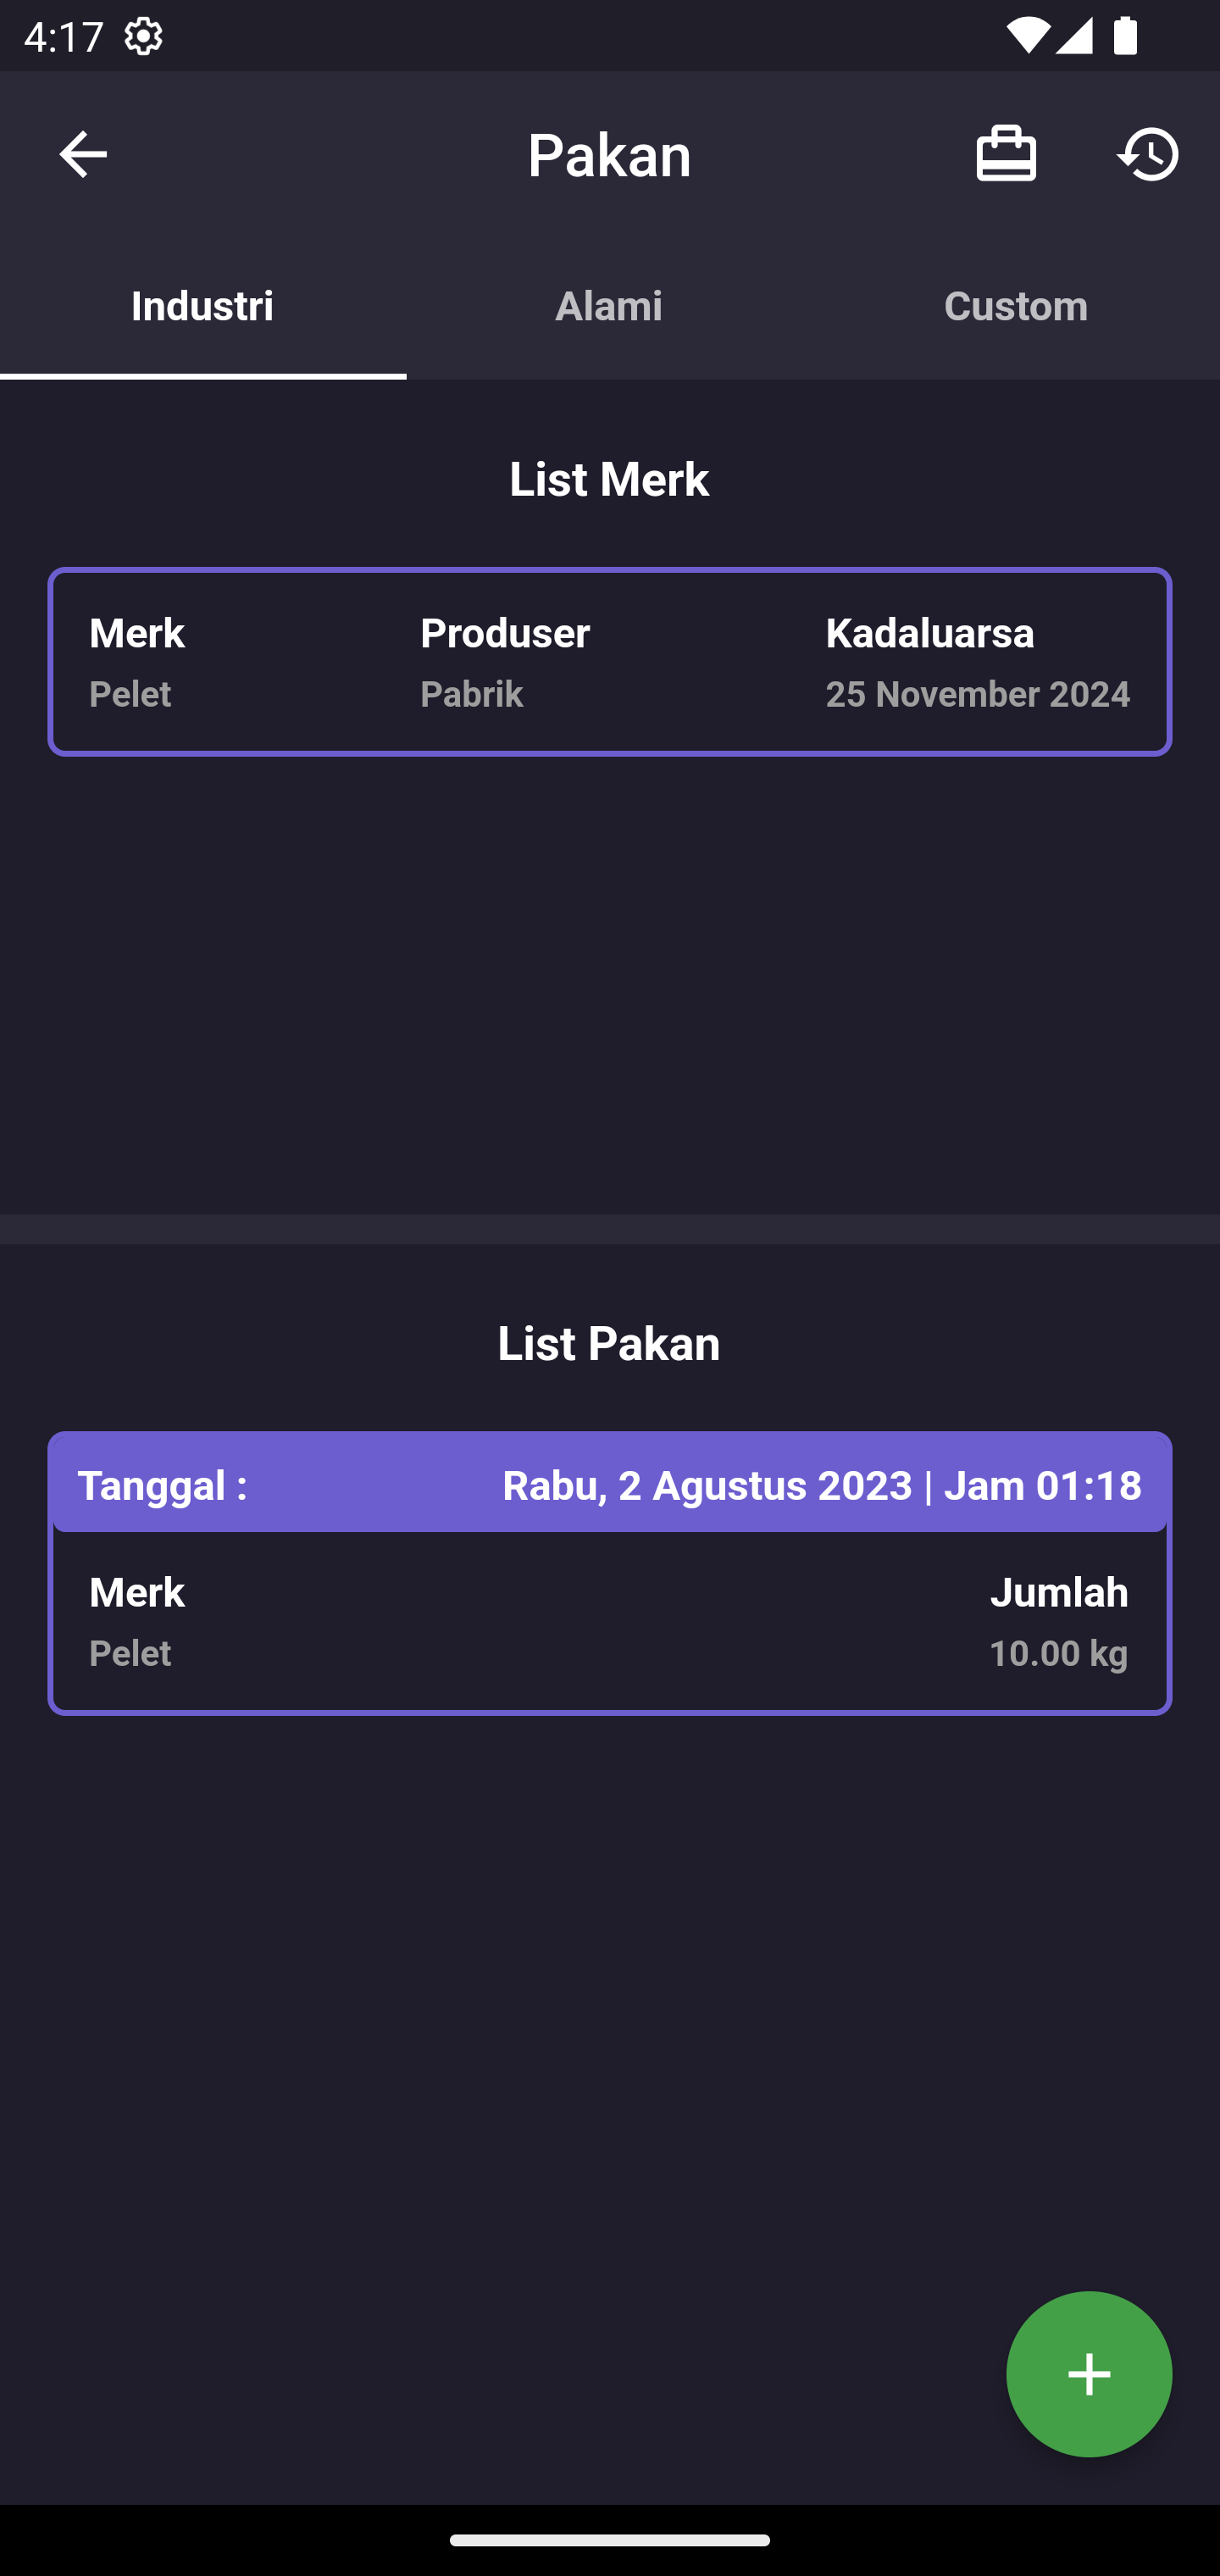
\includegraphics[width=\linewidth]{gambar/sprint4/inv_pakan.png}
						\caption{Halaman Inventaris Pakan}
					\endminipage\hfill
					\minipage{0.32\textwidth}
						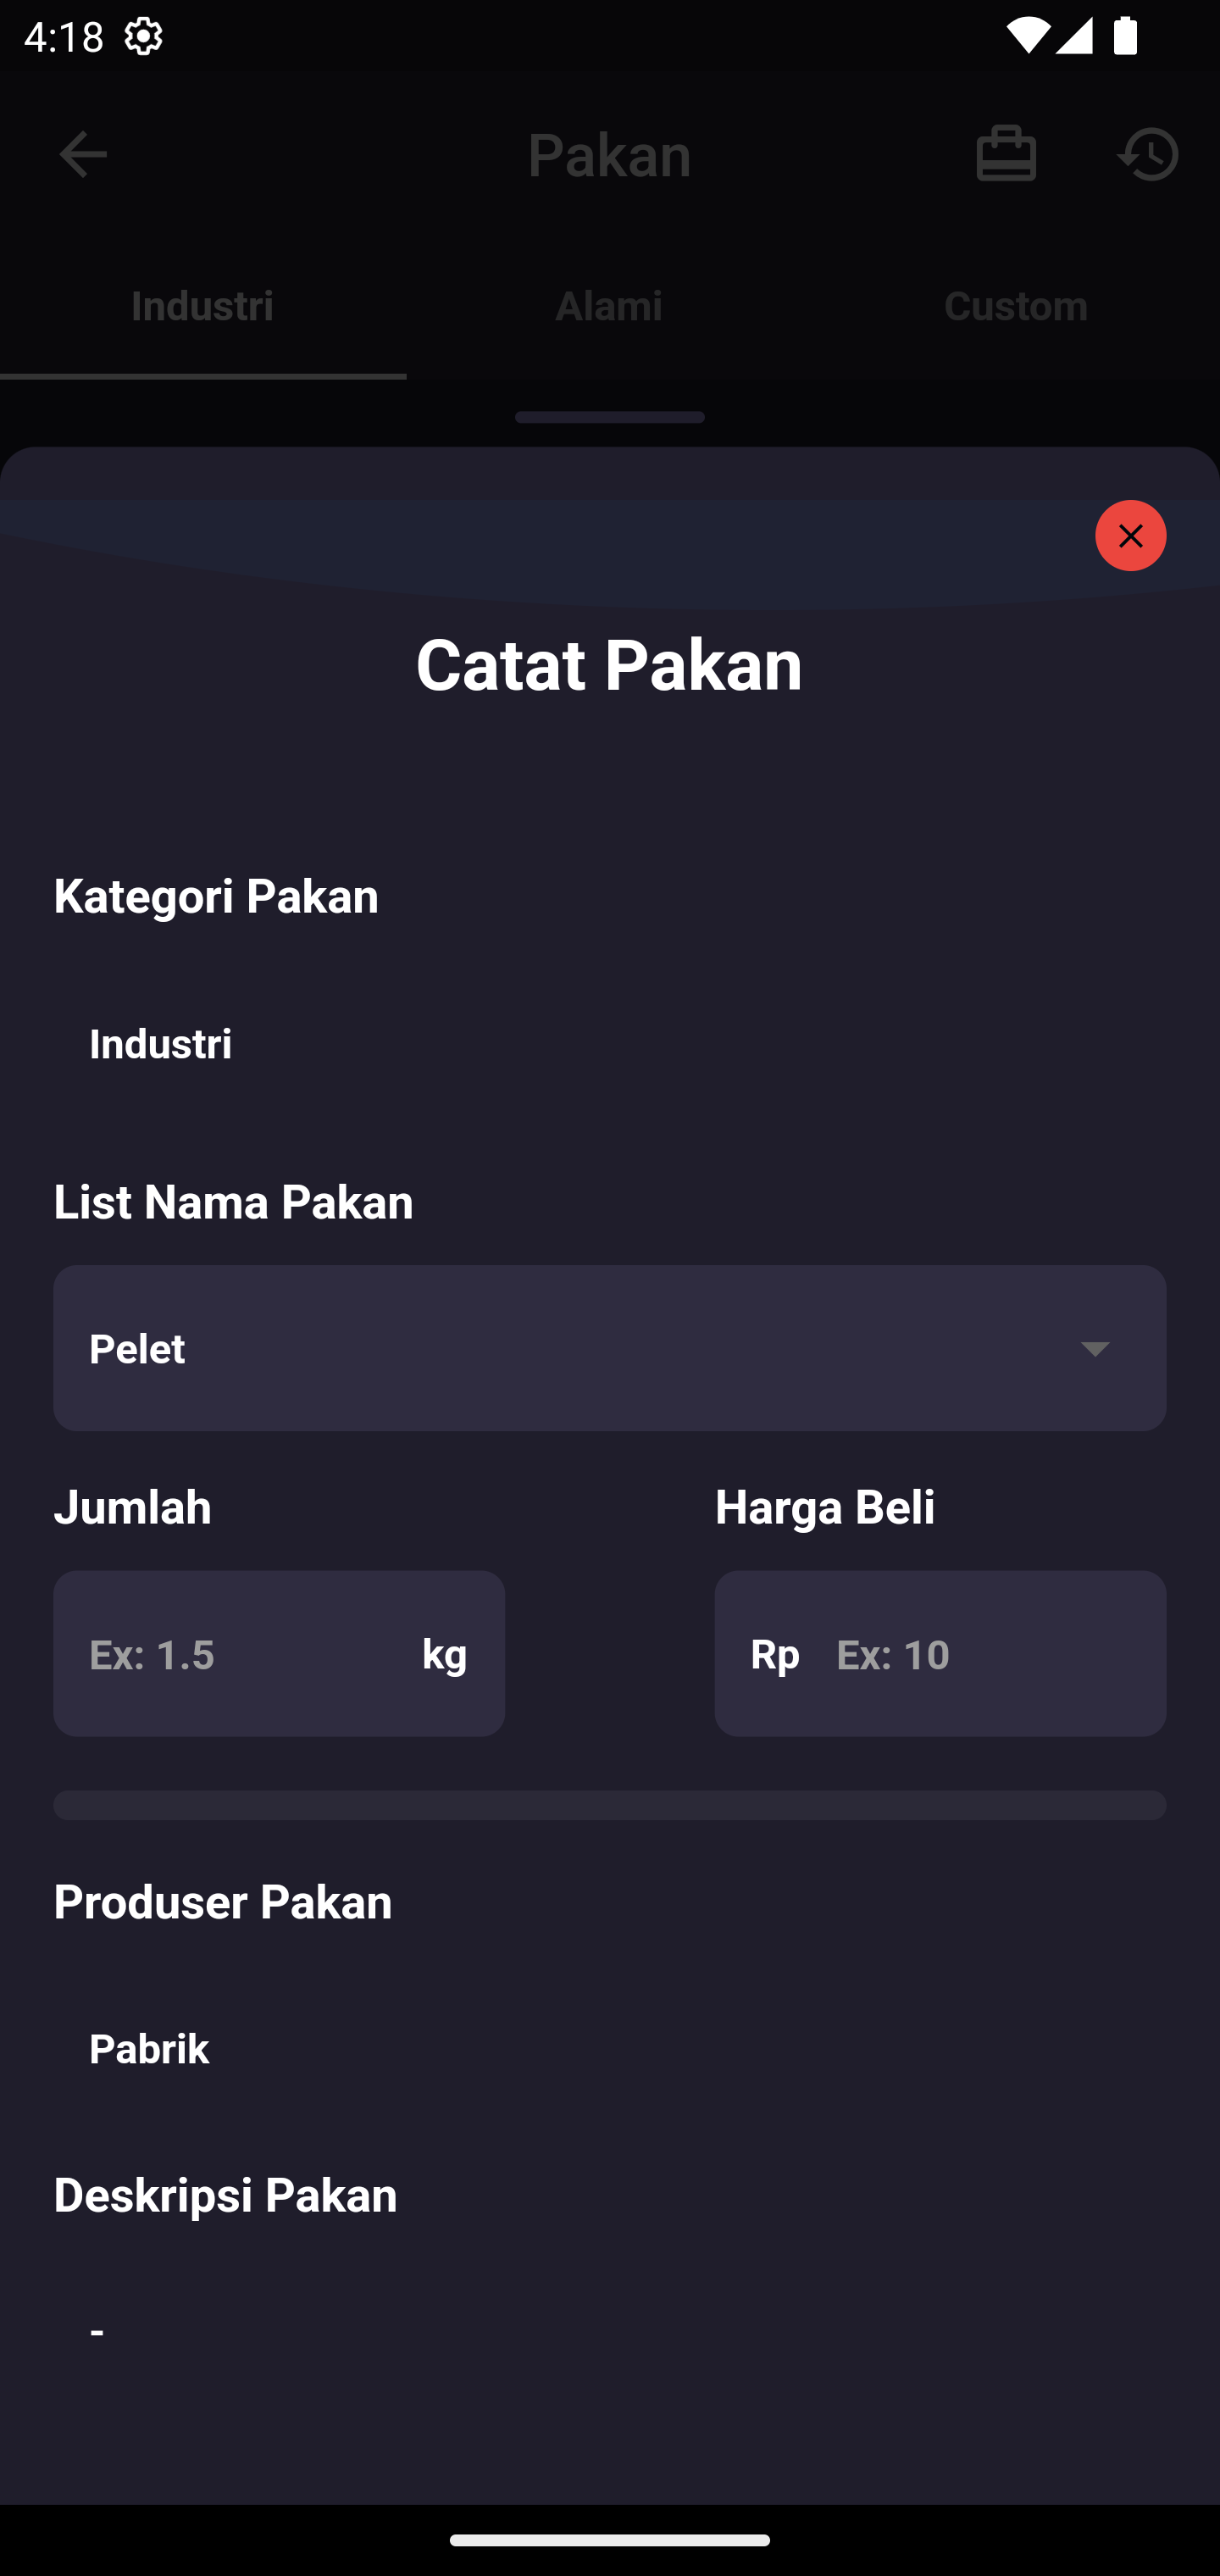
\includegraphics[width=\linewidth]{gambar/sprint4/input_inv_pakan.png}
						\caption{Halaman Input Inventaris Pakan}
					\endminipage\hfill
					\minipage{0.32\textwidth}
						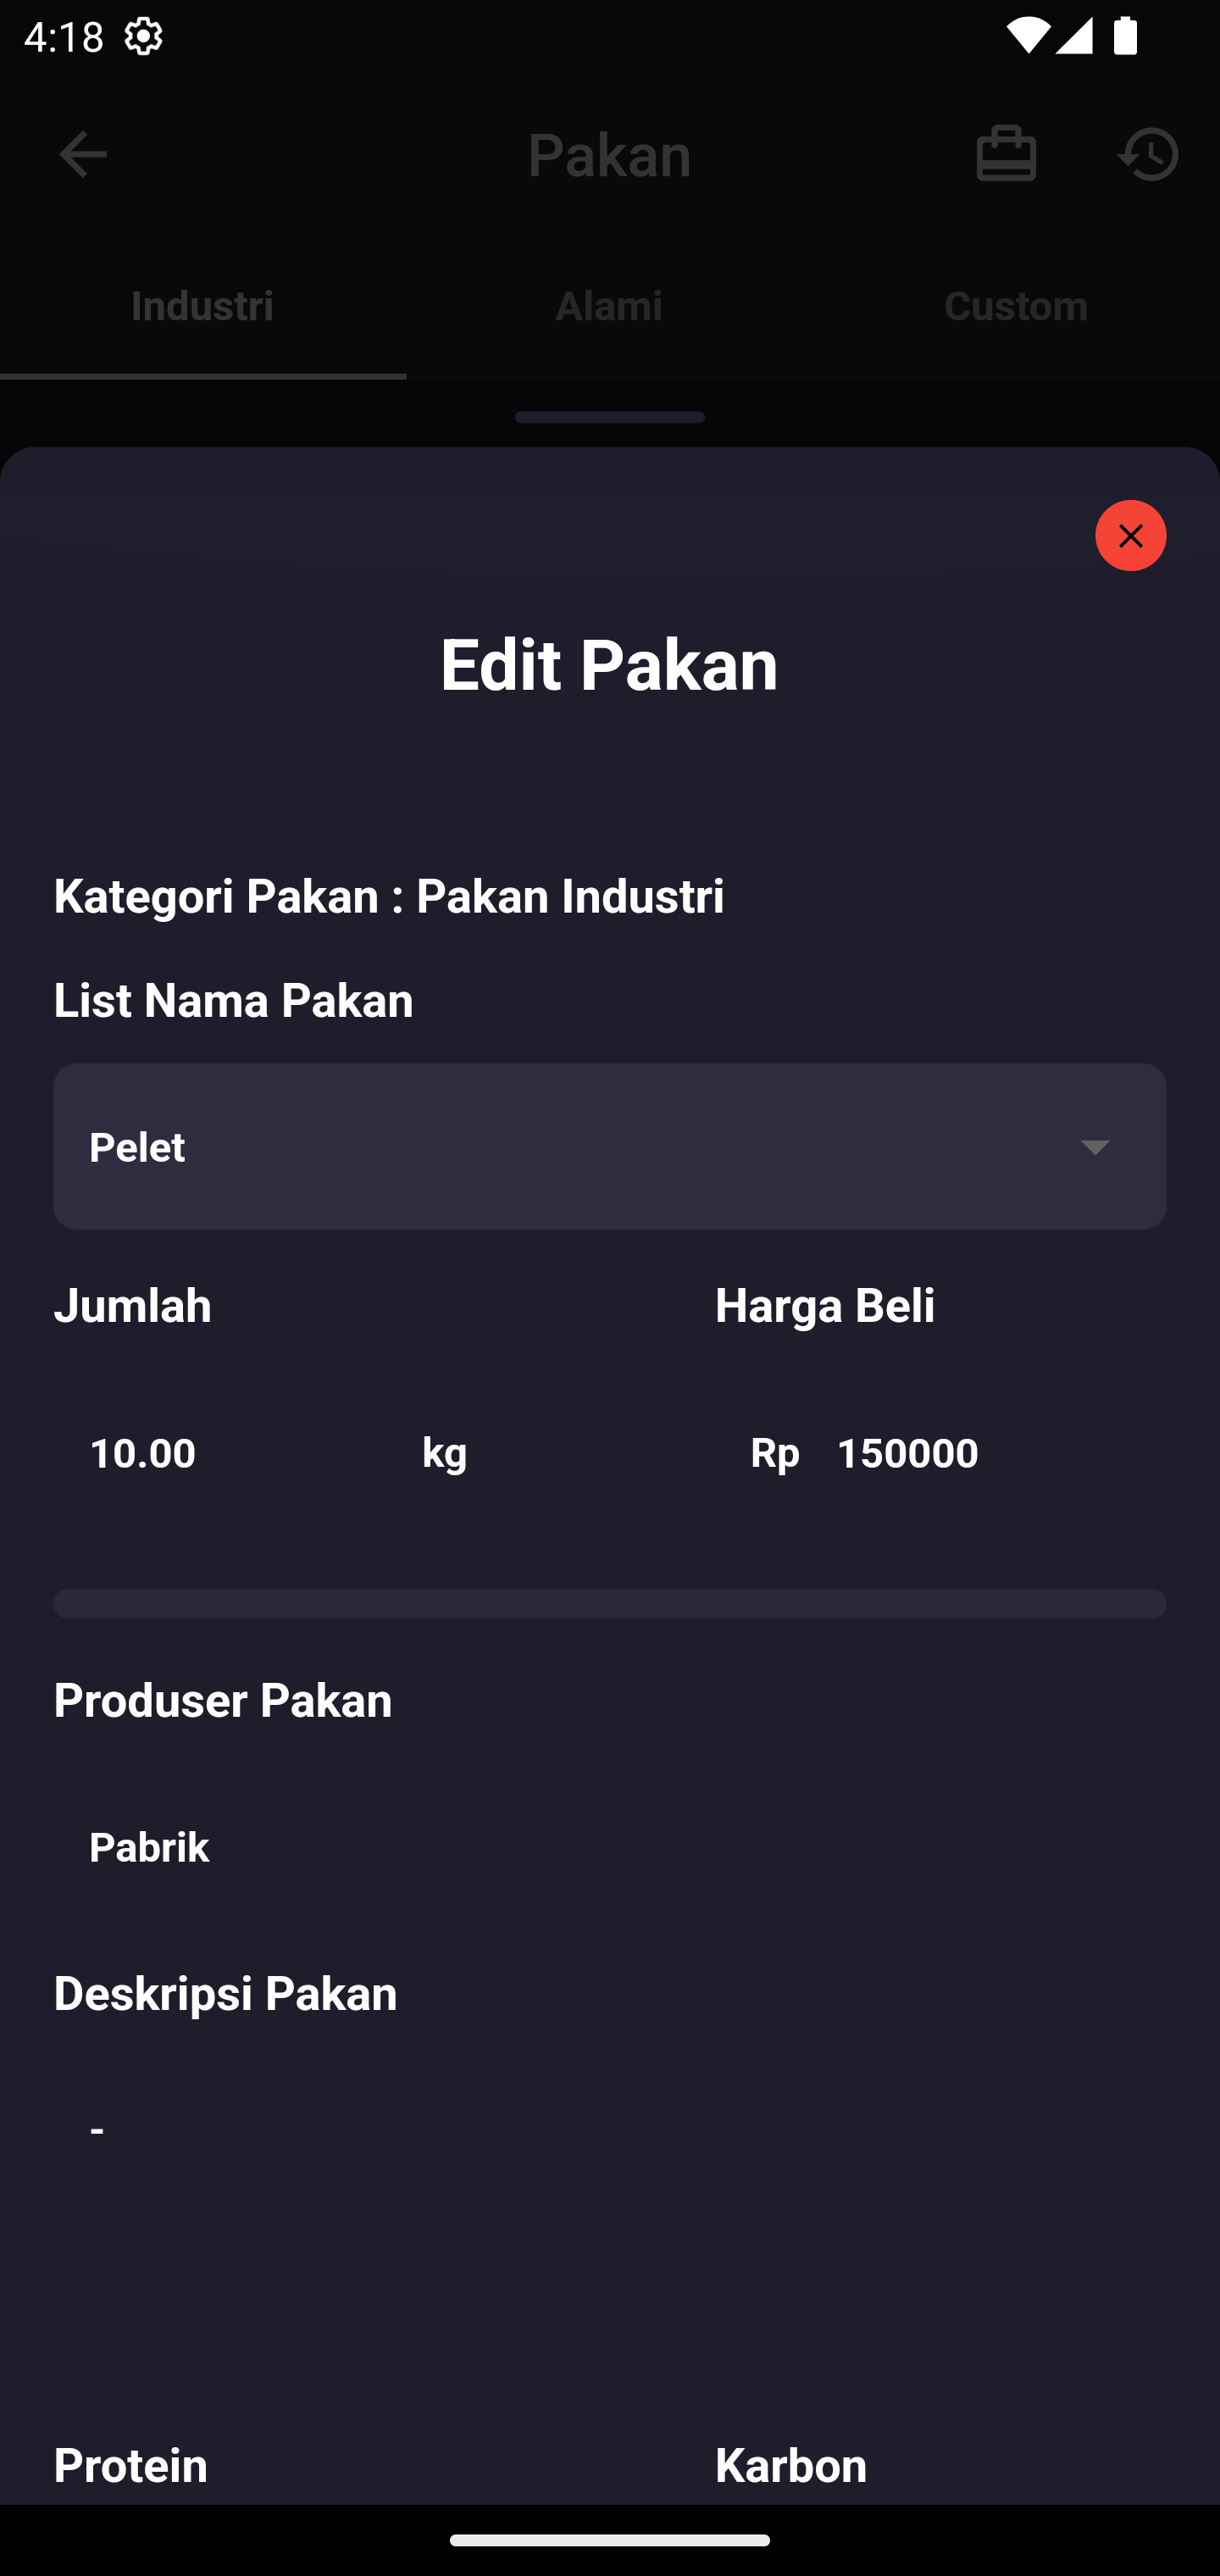
\includegraphics[width=\linewidth]{gambar/sprint4/detail_inv_pakan.png}
						\caption{Halaman Detail Inventaris Pakan}
					\endminipage\hfill
				\end{figure}

				Pada halaman inventaris pakan, dapat dilihat bahwa terdapat filter pakan yang berupa pakan industri, alami, dan Custom. Serta di bagian center terdapat dua bagian yang menampilkan list dari merk pakan dan pakan yang digunakan.

				Dibagian Catat Pakan, terdapat form isian yang harus dilengkapi jika ingin mencatat pakan. Kemudian, pada halaman Edit Pakan memiliki layout yang kurang lebih sama seperti Catat Pakan namun fungsi yang digunakan berbeda.

			\end{itemize}
		\end{enumerate}

		\item Design route dan penerapan pada Flutter untuk inventaris suplemen (dalam bentuk RESTful API)
		
		\begin{enumerate}
			\item Design Sample Route
			
			Berikut merupakan sample route yang sudah dibuat untuk inventaris suplemen.

			\begin{figure}[H]
				\centering
				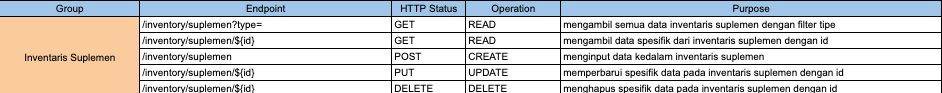
\includegraphics[width=1\textwidth]{gambar/sprint4/suplemen_sample_route.png}
				\caption{Sample Route Inventaris Suplemen}
			\end{figure}

			\item Model Backend
 			
			Berdasarkan sample route tersebut, dapat dibuat model dan class HTTP method pada backend. Berikut model serta class untuk inventaris suplemen :

			\begin{itemize}
				\item Model Inventaris Suplemen
				
				\begin{lstlisting}
					class SuplemenInventory(db.Document):
						id_int = db.SequenceField(required=True)
						farm_id = db.ReferenceField(Farm, required=True)
						function = db.StringField(required=True)
						name = db.StringField(required=True)
						description = db.StringField(required=True)
						price = db.IntField(required=True)
						amount = db.FloatField(required=True)
						type = db.StringField(required=True)
						min_expired_period = db.IntField(required=True)
						max_expired_period = db.IntField(required=True)
						image = db.StringField(required=True)
						created_at = db.DateTimeField(default=datetime.datetime.now)
						updated_at = db.DateTimeField(default=datetime.datetime.now)
				\end{lstlisting}
			\end{itemize}

			\item Fungsi-fungsi HTTP Method
			
			\begin{itemize}
				\item Mengambil semua data inventaris suplemen (HTTP Method - GET)
				
				\begin{lstlisting}
					class SuplemenInventoriesApi(Resource):
						@jwt_required()

						def get(self):
							try:
								current_user = get_jwt_identity()
								farm = str(current_user['farm_id'])
								farm_id = ObjectId(farm)
					
								type = request.args.get('type') if request.args.get('type') else ""
								name = request.args.get('name') if request.args.get('name') else ""
					
								pipeline = [
									{"$sort": {"id_int": 1}},
									{
										'$match': {
											"farm_id": farm_id,
											'function': {
												'$regex': type,
												'$options': 'i'
											}
										}
									},
									{
										'$match': {
											'name': {
												'$regex': name,
												'$options': 'i'
											}
										}
									}
								]
							
								testing = SuplemenInventory.objects.aggregate(pipeline)
								temp = list(testing)
								response = json.dumps({
									'status': 'success',
									'data': temp,
								}, default=str)
								return Response(response, mimetype="application/json", status=200)
							except Exception as e:
								response = {"message": e}
								response = json.dumps(response, default=str)
								return Response(response, mimetype="application/json", status=400)
				\end{lstlisting}

				\item Mengambil spesifik data inventaris pakan (HTTP Method - GET)
				
				\begin{lstlisting}
					class SuplemenInventoryApi(Resource):
						def get(self, id):
							try:
								pipeline = {"$match": {"id_int": int(id)}},
								testing = SuplemenInventory.objects.aggregate(pipeline)
								temp = list(testing)
								if len(temp) == 0:
									res = {"message": 'no data found'}
									response = json.dumps(res, default=str)
									return Response(response, mimetype="application/json", status=200)
								response = json.dumps({
									'status': 'success',
									'data': temp[0],
								}, default=str)
								return Response(response, mimetype="application/json", status=200)
							except Exception as e:
								response = {"message": e}
								response = json.dumps(response, default=str)
								return Response(response, mimetype="application/json", status=400)
				\end{lstlisting}

				\item Menambahkan data inventaris pakan (HTTP Method - POST)
				
				\begin{lstlisting}
					class SuplemenInventoriesApi(Resource):
						@jwt_required()
							def post(self):
								try:
									current_user = get_jwt_identity()
									farm = str(current_user['farm_id'])
									body = {
										"farm_id": farm,
										"function": request.form.get('function', None),
										"name": request.form.get('name', None),
										"description": request.form.get('description', None),
										"price": request.form.get('price', None),
										"amount": request.form.get('amount', None),
										"type": request.form.get('type', None),
										"min_expired_period": request.form.get('min_expired_period', None),
										"max_expired_period": request.form.get('max_expired_period', None),
										"image": request.form.get('image', None)
									}
									inventory = SuplemenInventory(**body).save()
									id = inventory.id
									res = {"message": "success add suplemen to inventory", "id": id, "data": body}
									response = json.dumps(res, default=str)
									return Response(response, mimetype="application/json", status=200)
								except Exception as e:
									response = {"message": str(e)}
									response = json.dumps(response, default=str)
									return Response(response, mimetype="application/json", status=400)
				\end{lstlisting}

				\item Memperbarui spesifik data inventaris pakan (HTTP Method - PUT)
				
				\begin{lstlisting}
					class SuplemenInventoryApi(Resource):
						def put(self, id):
							try:
								body = {
									"id_int": int(id),
									"function": request.form.get('function', None),
									"name": request.form.get('name', None),
									"description": request.form.get('description', None),
									"price": request.form.get('price', None),
									"amount": request.form.get('amount', None),
									"type": request.form.get('type', None),
									"min_expired_period": request.form.get('min_expired_period', None),
									"max_expired_period": request.form.get('max_expired_period', None),
									"image": request.form.get('image', None)
								}
								inventory = SuplemenInventory.objects.get(id_int = int(id)).update(**body)
								response = {"message": "success update suplemen inventory", "data": body}
								response = json.dumps(response, default=str)
								return Response(response, mimetype="application/json", status=200)
							except Exception as e:
								response = {"message": str(e)}
								response = json.dumps(response, default=str)
								return Response(response, mimetype="application/json", status=400)
				\end{lstlisting}

				\item Menghapus spesifik data inventaris pakan (HTTP Method - DELETE)
				
				\begin{lstlisting}
					class SuplemenInventoryApi(Resource):
						def delete(self, id):
							try:
								inventory = SuplemenInventory.objects.get(id_int = int(id)).delete()
								response = {"message": "success delete suplemen inventory"}
								response = json.dumps(response, default=str)
								return Response(response, mimetype="application/json", status=200)
							except Exception as e:
								response = {"message": str(e)}
								response = json.dumps(response, default=str)
								return Response(response, mimetype="application/json", status=400)
				\end{lstlisting}
			\end{itemize}

			\item Controller HTTP pada Flutter
			
			\begin{itemize}
				\item Mengambil semua data inventaris suplemen (HTTP Method - GET)
				
				\begin{lstlisting}
					Future getAllData(String type, Function() doAfter) async {
						suplemenList.value.data!.clear();
						isLoadingPage.value = true;
						isProbLoading.value = true;
						isCarbLoading.value = true;
						listCarbon.clear();
						listCultureProbiotik.clear();

						SharedPreferences prefs = await SharedPreferences.getInstance();
						String token = prefs.getString('token').toString();
						var headers = {'Authorization': 'Bearer $token'};

						final response = await http.get(
						Uri.parse('${Urls.invSup}?type=$type'),
						headers: headers,
						);

						try {
						if (response.statusCode == 200) {
							InventarisSuplemenModel res =
								InventarisSuplemenModel.fromJson(jsonDecode(response.body));

							suplemenList.value = res;
							// inspect(suplemenList.value.data);

							if (suplemenList.value.data!.isNotEmpty) {
							for (var i in suplemenList.value.data!) {
								if (type == 'Probiotik') {
								listCultureProbiotik.add({
									'id': i.idInt,
									'suplemen_id': i.sId,
									'suplemen_name': i.name,
								});

								selectedCultureProbiotik.value = listCultureProbiotik[0];
								}
								if (type == 'Feed Additive') {
								listCarbon.add({
									'id': i.idInt,
									'suplemen_id': i.sId,
									'suplemen_name': i.name,
								});

								selectedCarbon.value = listCarbon[0];
								}
							}
							}

							// inspect(listCultureProbiotik);

							doAfter();
						}
						} catch (e) {
						inspect(e);
						throw Exception(e);
						}
						isProbLoading.value = false;
						isCarbLoading.value = false;
						isLoadingPage.value = false;
					}
				\end{lstlisting}

				\item Mengambil spesifik data inventaris suplemen (HTTP Method - GET)
				
				\begin{lstlisting}
					Future getDataByID(int id, Function() doAfter) async {
						isLoadingDetail.value = true;

						final response = await http.get(Uri.parse('${Urls.invSup}/$id'));

						try {
						if (response.statusCode == 200) {
							DetailInventarisSuplemenModel res =
								DetailInventarisSuplemenModel.fromJson(jsonDecode(response.body));

							// for (var i in listSuplemenName) {
							//   if (i['suplemen_name_id'] == res.data.fee)
							// }

							functionCategory.value = res.data!.function!.toString();
							name.text = res.data!.name!.toString();
							selectedFeedAdditive.value = res.data!.name!.toString();
							desc.text = res.data!.description.toString();
							price.text = res.data!.price.toString();
							amount.text = res.data!.amount!.toStringAsFixed(2);
							typeCategory.value = res.data!.type.toString();
							minExp.text = res.data!.minExpiredPeriod.toString();
							maxExp.text = res.data!.maxExpiredPeriod.toString();
							image.value = res.data!.image.toString();
						}
						doAfter();
						} catch (e) {
						throw Exception(e);
						}
						isLoadingDetail.value = false;
					}
				\end{lstlisting}

				\item Menambahkan data inventaris suplemen (HTTP Method - POST)
				
				\begin{lstlisting}
					Future postData(Function() doAfter) async {
						var map = <String, dynamic>{};

						SharedPreferences prefs = await SharedPreferences.getInstance();
						String token = prefs.getString('token').toString();
						var headers = {'Authorization': 'Bearer $token'};

						map['function'] = functionCategory.value;
						map['name'] = functionCategory.value == 'Feed Additive'
							? selectedFeedAdditive.value
							: name.text;
						map['description'] = desc.text == '' ? '-' : desc.text;
						map['price'] = price.text;
						map['amount'] = amount.text.replaceAll(',', '.');
						map['type'] = typeCategory.value;
						map['min_expired_period'] = minExp.text == '' ? '0' : minExp.text;
						map['max_expired_period'] = maxExp.text == ''
							? (int.parse(minExp.text == '' ? '0' : minExp.text) * 2).toString()
							: maxExp.text;
						map['image'] = image.value;

						isLoadingPost.value = true;

						inspect(map);

						try {
						await http.post(
							Uri.parse(Urls.invSup),
							body: map,
							headers: headers,
						);
						doAfter();
						} catch (e) {
						throw Exception(e);
						}
						isLoadingPost.value = false;
					}

				\end{lstlisting}

				\item Memperbarui spesifik data inventaris suplemen (HTTP Method - PUT)
				
				\begin{lstlisting}
					Future updateData(int id, Function() doAfter) async {
						var map = <String, dynamic>{};

						inspect(id);

						map['function'] = functionCategory.value;
						map['name'] = functionCategory.value == 'Feed Additive'
							? selectedFeedAdditive.value
							: name.text;
						map['description'] = desc.text == '' ? '-' : desc.text;
						map['price'] = price.text;
						map['amount'] = amount.text.replaceAll(',', '.');
						map['type'] = typeCategory.value;
						map['min_expired_period'] = minExp.text == '' ? '0' : minExp.text;
						map['max_expired_period'] = maxExp.text == ''
							? (int.parse(minExp.text == '' ? '0' : minExp.text) * 2).toString()
							: maxExp.text;
						map['image'] = image.value;

						isLoadingPost.value = true;

						try {
						inspect(map);
						final res = await http.put(
							Uri.parse('${Urls.invSup}/$id'),
							body: map,
						);
						inspect(res);
						doAfter();
						} catch (e) {
						throw Exception(e);
						}
						isLoadingPost.value = false;
					}
				\end{lstlisting}

				\item Menghapus spesifik data inventaris suplemen (HTTP Method - DELETE)
				
				\begin{lstlisting}
					Future deleteData(int id, Function() doAfter) async {
						isLoadingDelete.value = true;
						try {
						  await http.delete(
							Uri.parse(
							  '${Urls.invSup}/$id',
							),
							headers: {
							  'Content-Type': 'application/json; charset=UTF-8',
							},
						  );
						  doAfter();
						} catch (e) {
						  throw Exception(e);
						}
						isLoadingDelete.value = false;
					 }
				\end{lstlisting}
			\end{itemize}

			\item Tampilan pada Flutter
			
			\begin{itemize}
				\item Halaman Inventaris Suplemen, Input Suplemen, dan Detail Suplemen
				
				\begin{figure}[H]
					\minipage{0.32\textwidth}
						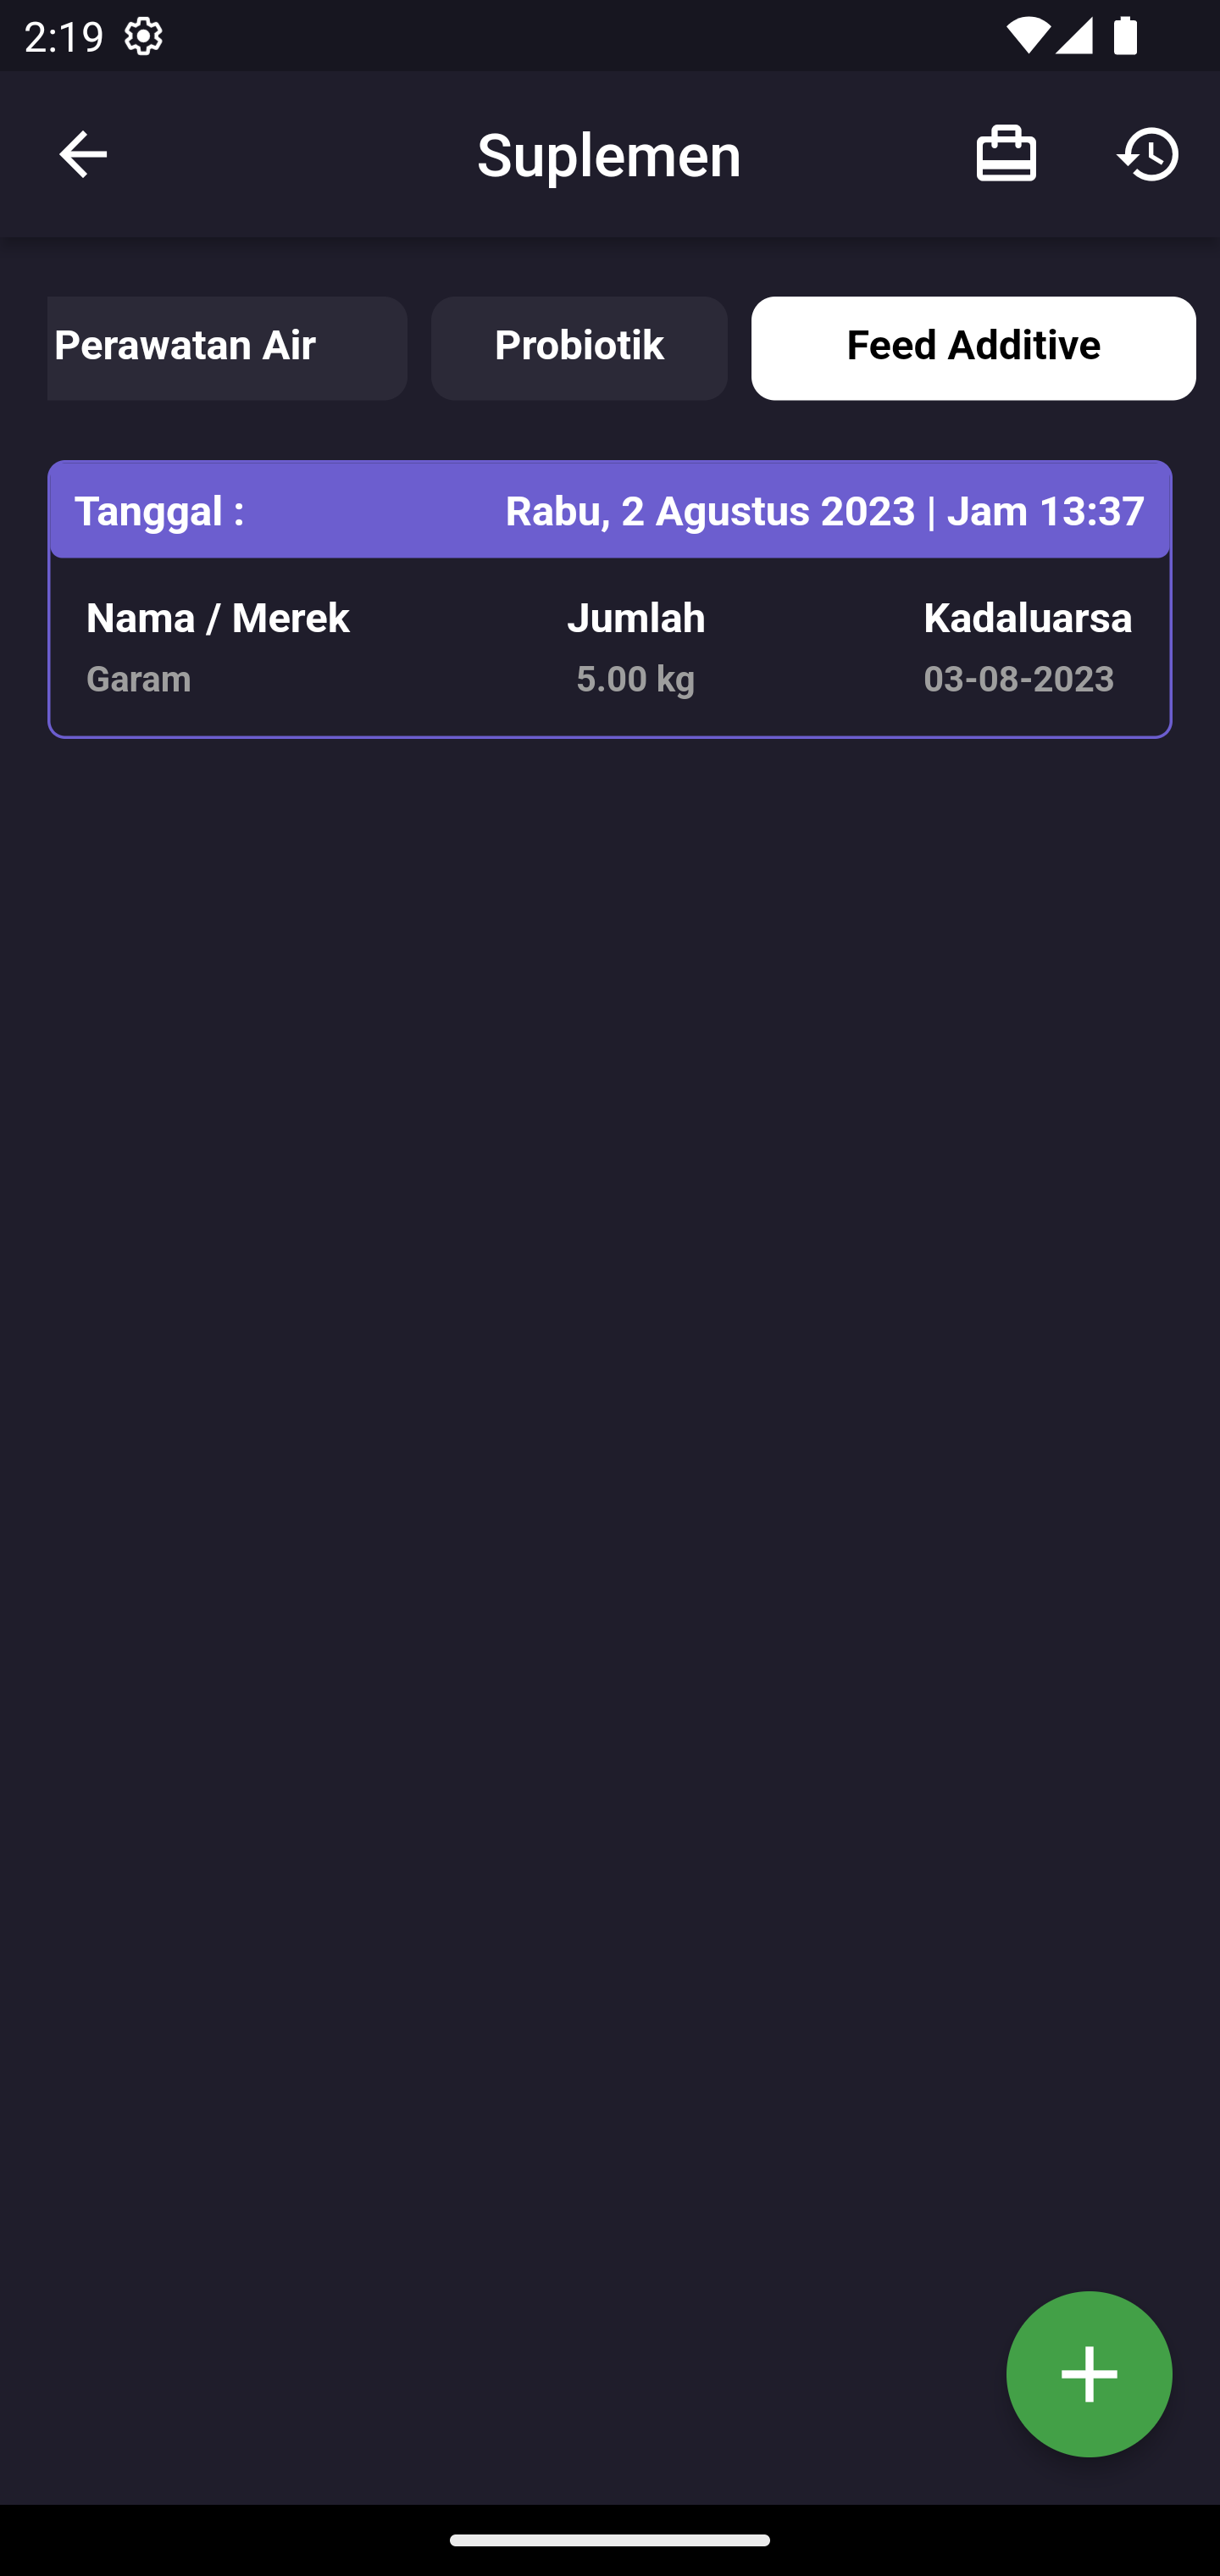
\includegraphics[width=\linewidth]{gambar/sprint4/sup_1.png}
						\caption{Halaman Inventaris Suplemen}
					\endminipage\hfill
					\minipage{0.32\textwidth}
						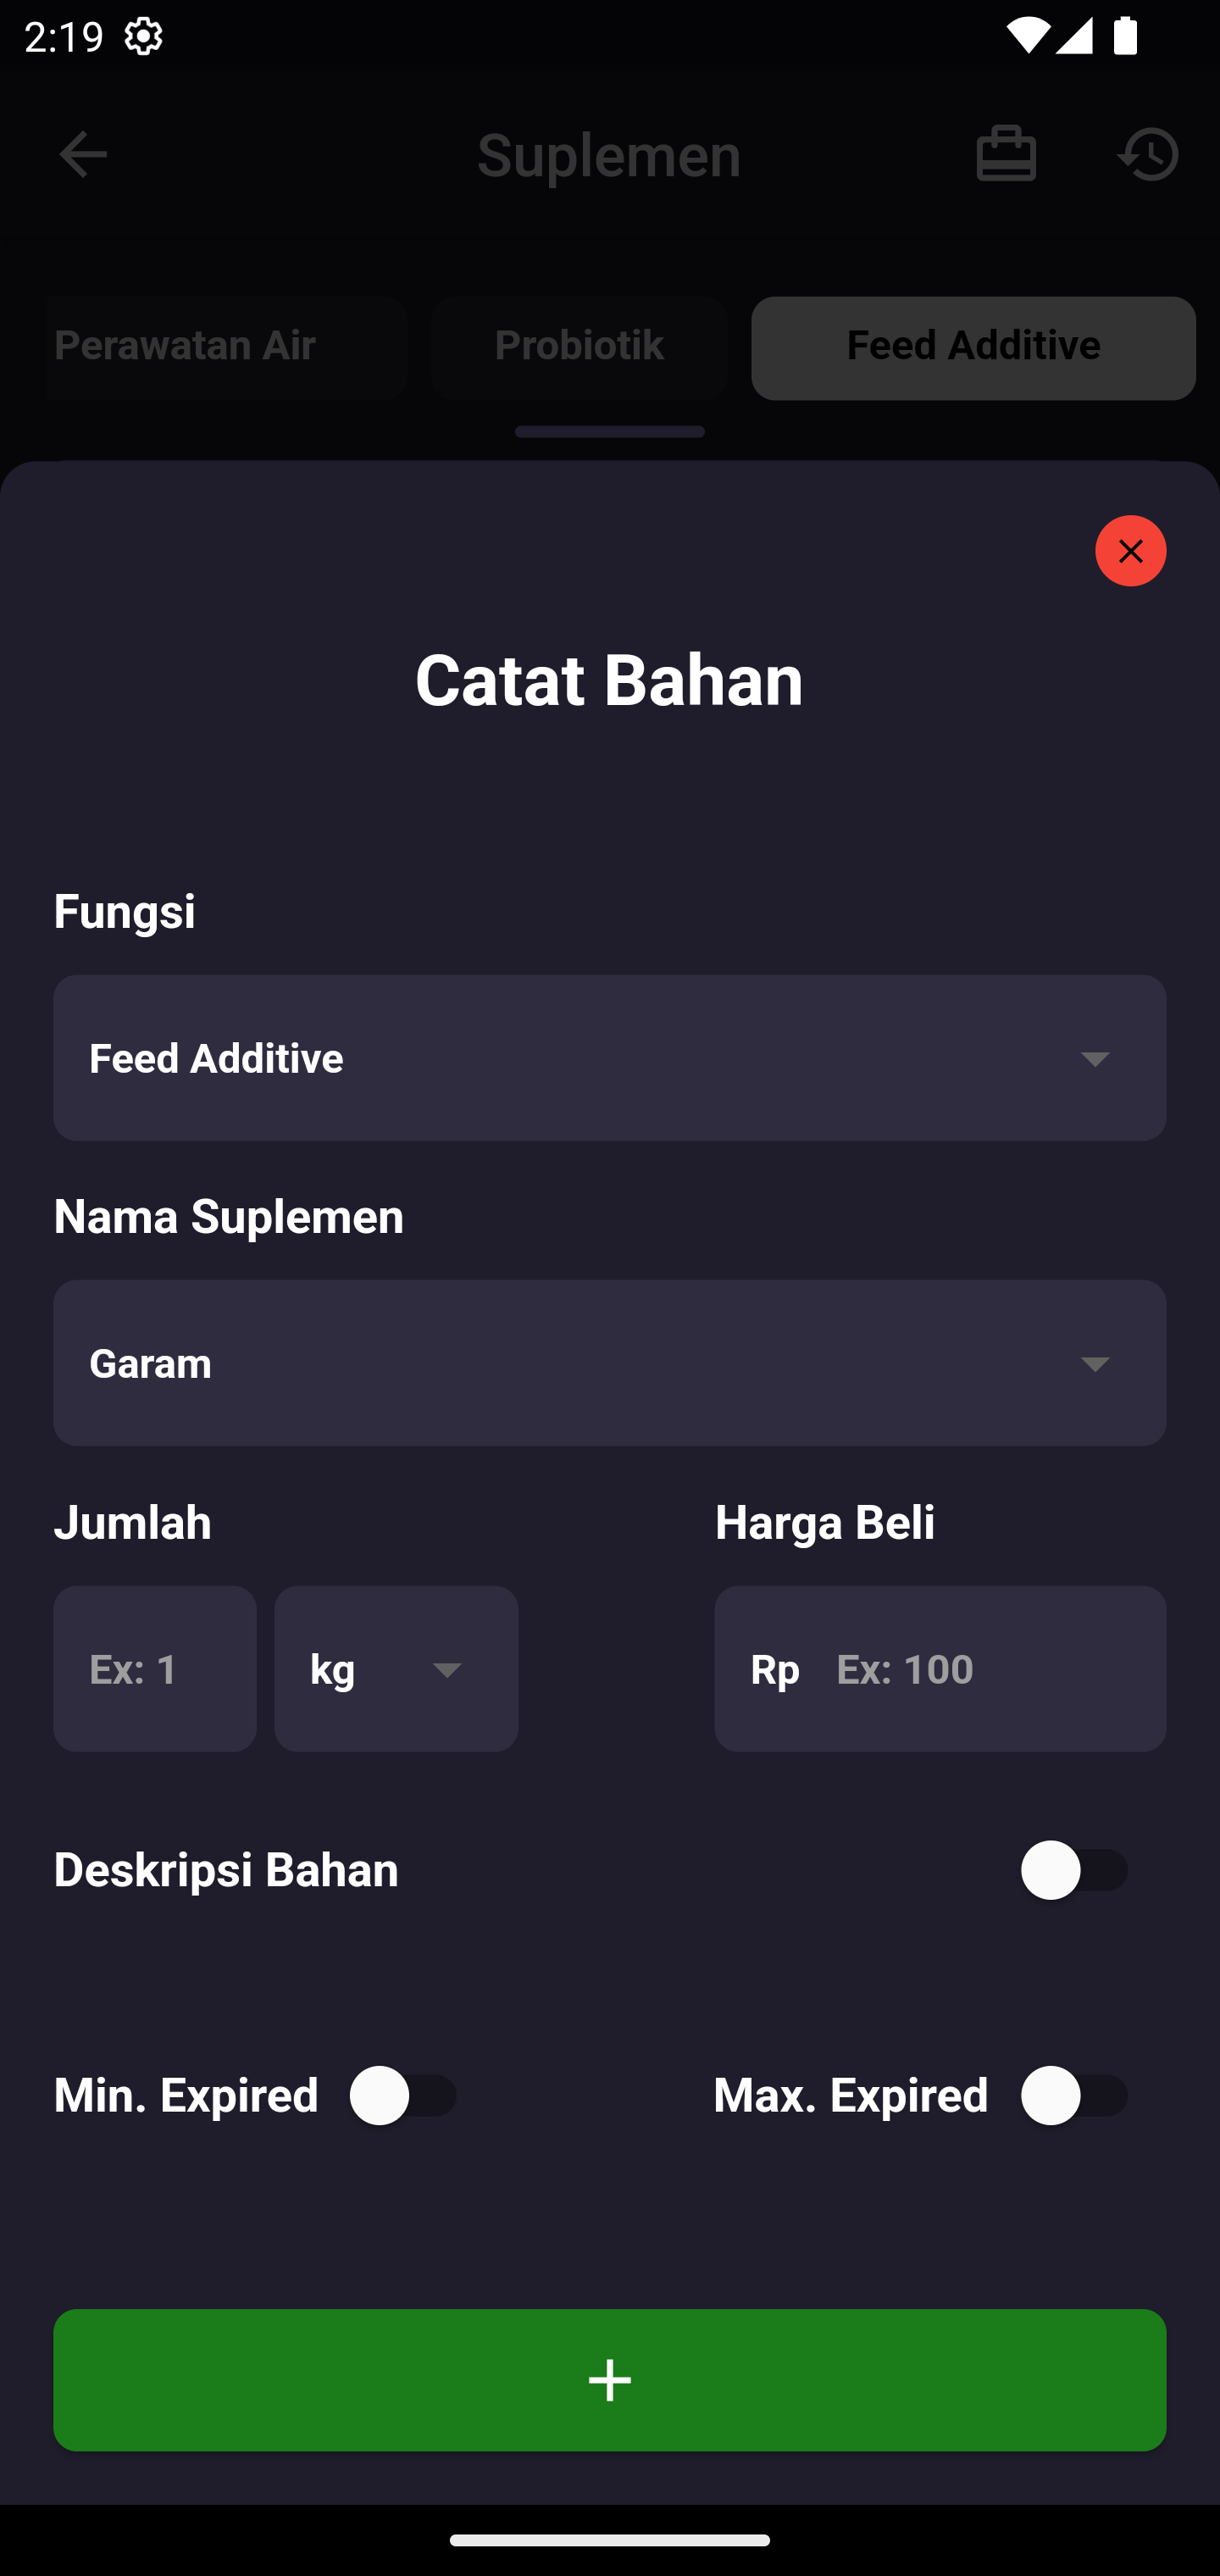
\includegraphics[width=\linewidth]{gambar/sprint4/sup_2.png}
						\caption{Halaman Input Inventaris Suplemen}
					\endminipage\hfill
					\minipage{0.32\textwidth}
						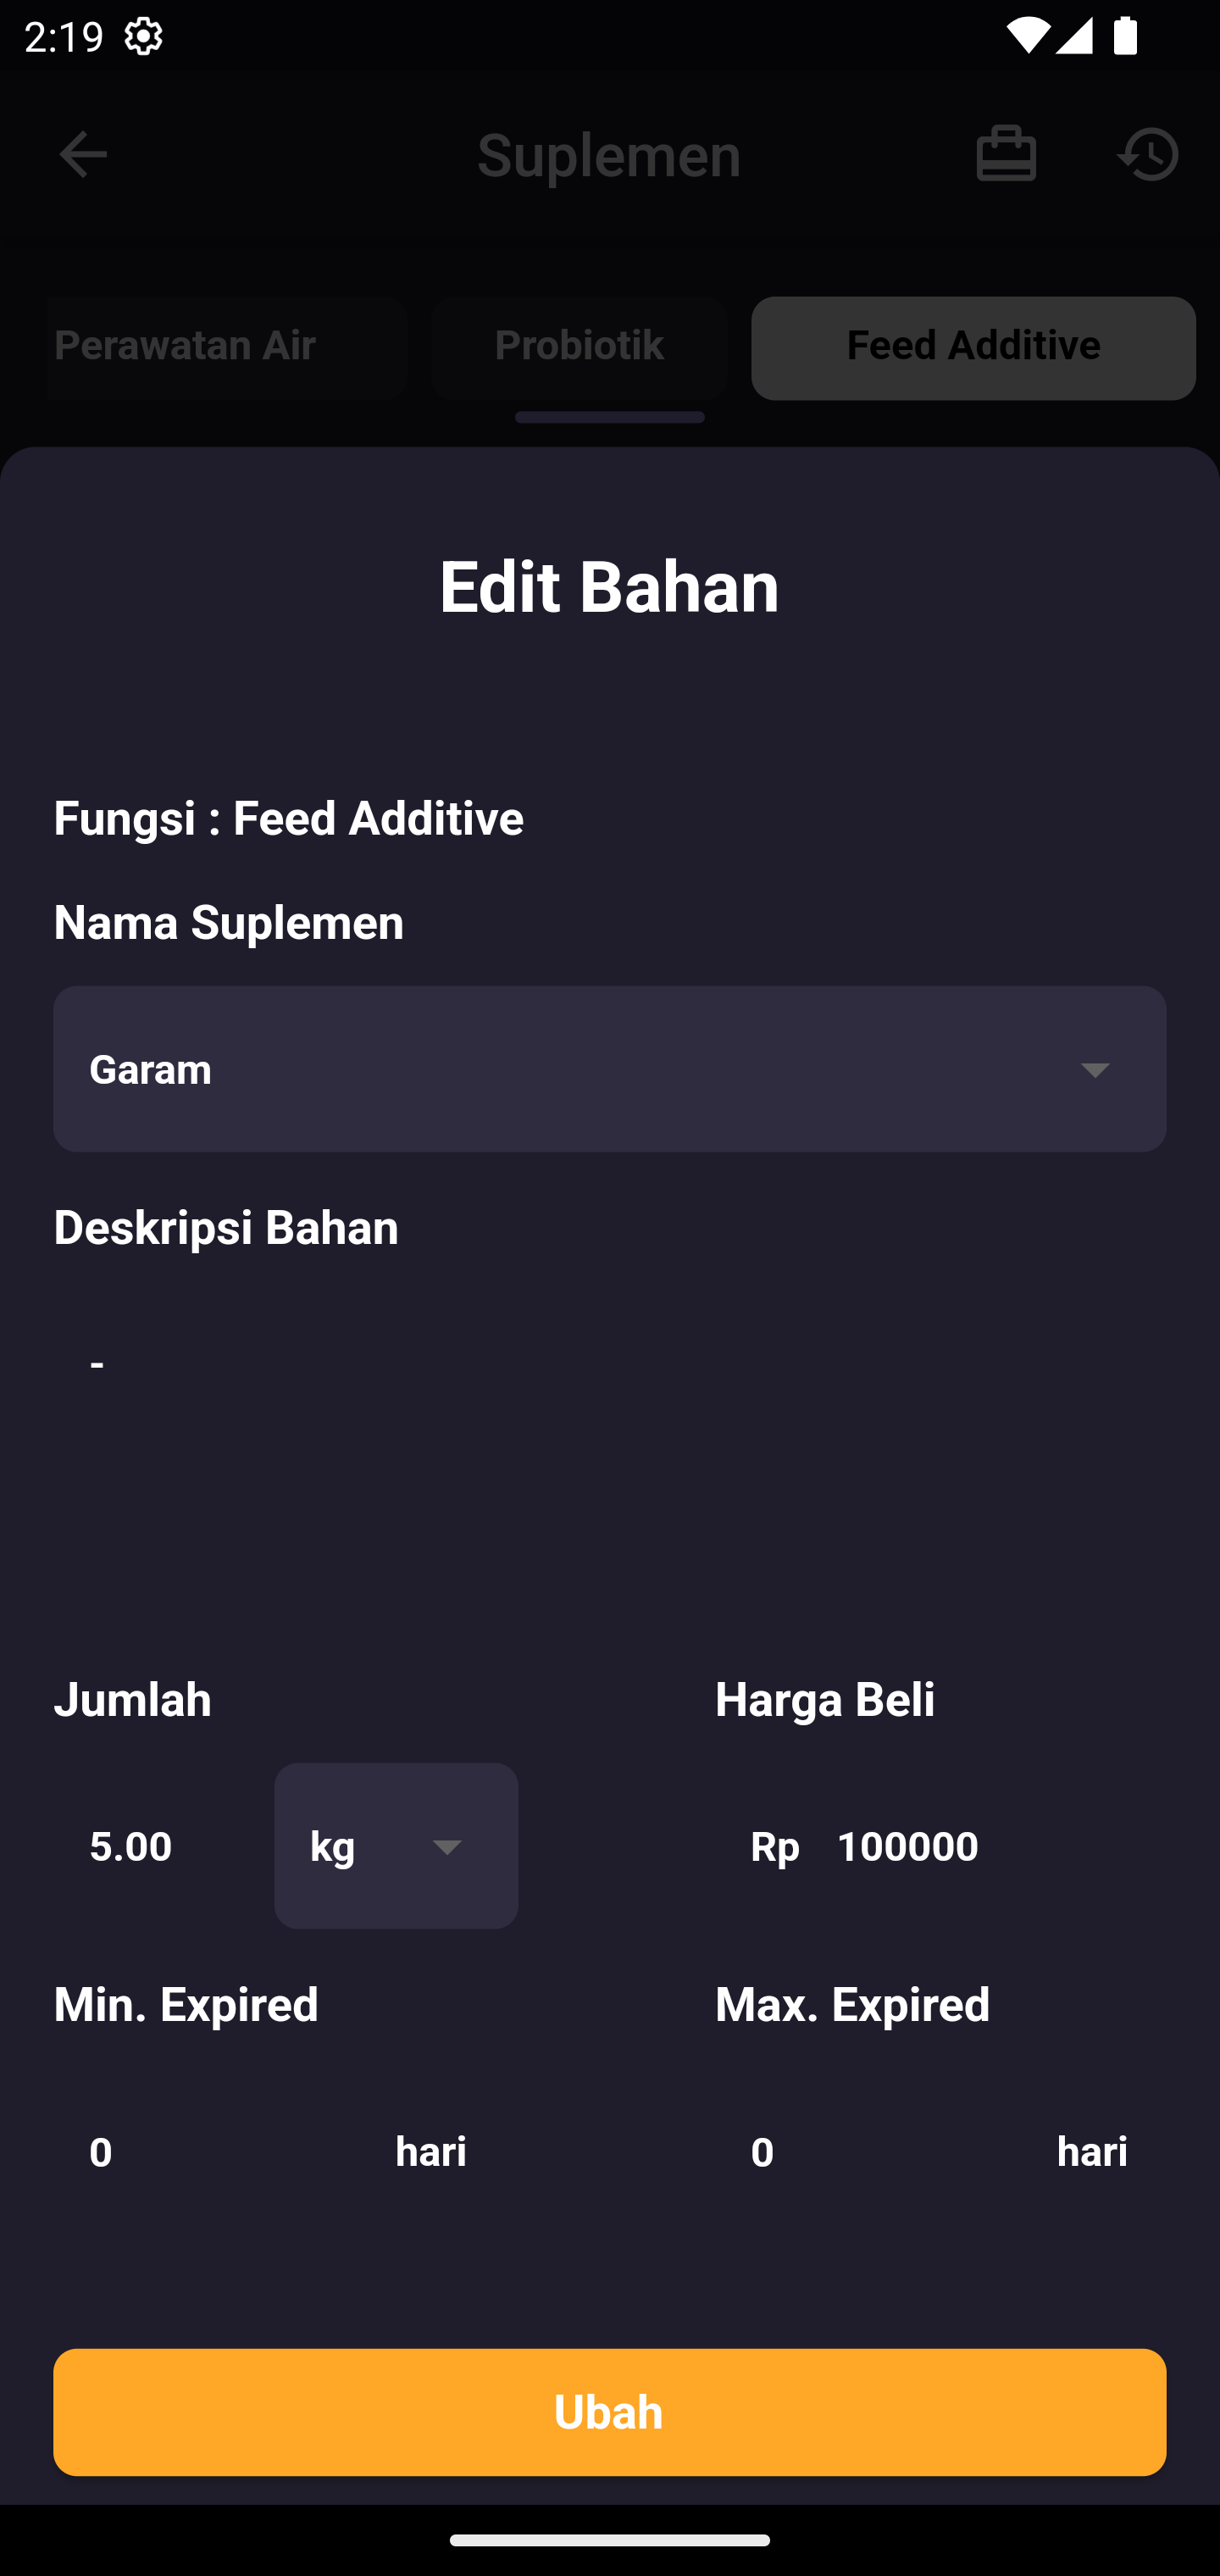
\includegraphics[width=\linewidth]{gambar/sprint4/sup_3.png}
						\caption{Halaman Detail Inventaris Suplemen}
					\endminipage\hfill
				\end{figure}

				Pada Halaman inventaris suplemen, dapat dilihat bahwa terdapat beberapa filter suplemen seperti Feed Additive, Probiotik, Perawatan Air, dan Obat . Serta di bagian center terdapat list dari inventaris suplemen yang sudah terdaftar.

				Dibagian Catat suplemen, terdapat form isian yang harus dilengkapi jika ingin mencatat suplemen. Kemudian, pada halaman Edit Suplemen memiliki layout yang kurang lebih sama seperti Catat Suplemen namun fungsi yang digunakan berbeda.
			\end{itemize}
		\end{enumerate}

		\item Design route dan penerapan pada Flutter untuk inventaris listrik (dalam bentuk RESTful API) 
		
		\begin{enumerate}
			\item Design Sample Route
			
			Berikut merupakan sample route yang sudah dibuat untuk inventaris pakan.

			\begin{figure}[H]
				\centering
				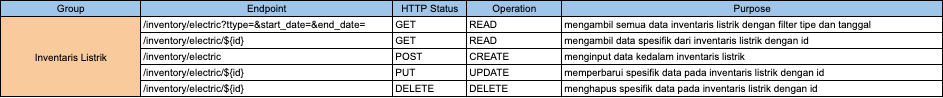
\includegraphics[width=1\textwidth]{gambar/sprint4/sample_route_electric.png}
				\caption{Sample Route Inventaris Listrik}
			\end{figure}

			\item Model Backend
 			
			Berdasarkan sample route tersebut, dapat dibuat model dan class HTTP method pada backend. Berikut model serta class untuk inventaris listrik :

			\begin{itemize}
				\item Model Inventaris Listrik
				
				\begin{lstlisting}
					class ElectricInventory(db.Document):
						id_int = db.SequenceField(required=True)
						farm_id = db.ReferenceField(Farm, required=True)
						type = db.StringField(required=True)
						name = db.StringField(required=True)
						daya = db.StringField()
						price = db.IntField(required=True)
						id_token = db.StringField()
						month = db.StringField()
						image = db.StringField(required=True)
						created_at = db.DateTimeField(default=datetime.datetime.now)
						updated_at = db.DateTimeField(default=datetime.datetime.now)
				\end{lstlisting}

				% Pada model tersebut, terdapat beberapa \textit{key} seperti feed\_name\_id yang digunakan untuk mereferensikan kepada tabel FeedName, farm\_id untuk mereferensikan kepada tabel Farm, id\_int untuk 

				\end{itemize}

			\item Fungsi-fungsi HTTP Method
			
			\begin{itemize}
				\item Mengambil semua data inventaris listrik (HTTP Method - GET)
				
				\begin{lstlisting}
					class ElectricInventoriesApi(Resource):
						@jwt_required()

						def get(self):
							try:
								current_user = get_jwt_identity()
								farm = str(current_user['farm_id'])
								farm_id = ObjectId(farm)
					
								start_date = datetime.datetime.strptime(request.args.get('start_date'), '%Y-%m-%d') if request.args.get('start_date') else datetime.datetime.strptime("2023-01-01", '%Y-%m-%d')
								end_date = datetime.datetime.strptime(request.args.get('end_date'), '%Y-%m-%d') + datetime.timedelta(days=1) if request.args.get('end_date') else datetime.datetime.strptime("2030-01-01", '%Y-%m-%d')
								type = request.args.get('type') if request.args.get('type') else ""
					
								pipeline = [
									{"$sort": {"id_int": 1}},
									{
										'$match': {
											'created_at': {
												'$gte': start_date,
												'$lte': end_date,
											}
										}
									},
									{
										'$match': {
											"farm_id": farm_id,
											'type': {
												'$regex': type,
												'$options': 'i'
											}
										}
									}
								]
							
								testing = ElectricInventory.objects.aggregate(pipeline)
								temp = list(testing)
								response = json.dumps({
									'status': 'success',
									'data': temp,
								}, default=str)
								return Response(response, mimetype="application/json", status=200)
							except Exception as e:
								response = {"message": e}
								response = json.dumps(response, default=str)
								return Response(response, mimetype="application/json", status=400)
				\end{lstlisting}

				\item Mengambil spesifik data inventaris listrik (HTTP Method - GET)
				
				\begin{lstlisting}
					class ElectricInventoryApi(Resource):
						def get(self, id):
							try:
								pipeline = {"$match": {"id_int": int(id)}},
								testing = ElectricInventory.objects.aggregate(pipeline)
								temp = list(testing)
								if len(temp) == 0:
									res = {"message": 'no data found'}
									response = json.dumps(res, default=str)
									return Response(response, mimetype="application/json", status=200)
								response = json.dumps({
									'status': 'success',
									'data': temp[0],
								}, default=str)
								return Response(response, mimetype="application/json", status=200)
							except Exception as e:
								response = {"message": e}
								response = json.dumps(response, default=str)
								return Response(response, mimetype="application/json", status=400)
				\end{lstlisting}

				\item Menambahkan data inventaris listrik (HTTP Method - POST)
				
				\begin{lstlisting}
					class ElectricInventoriesApi(Resource):
						@jwt_required()
						def post(self):
							try:
								current_user = get_jwt_identity()
								farm = str(current_user['farm_id'])
								body = {
									"farm_id": farm,
									"name": request.form.get('name', None),
									"price": request.form.get('price', None),
									"type": request.form.get('type', None),
									"daya": request.form.get('daya', None),
									"image": request.form.get('image', None),
									"id_token": request.form.get('id_token', None),
									"month": request.form.get('month', None)
								}
								inventory = ElectricInventory(**body).save()
								id = inventory.id
								res = {"message": "success add electric to inventory", "id": id, "data": body}
								response = json.dumps(res, default=str)
								return Response(response, mimetype="application/json", status=200)
							except Exception as e:
								response = {"message": str(e)}
								response = json.dumps(response, default=str)
								return Response(response, mimetype="application/json", status=400)
				\end{lstlisting}

				\item Memperbarui spesifik data inventaris listrik (HTTP Method - PUT)
				
				\begin{lstlisting}
					class ElectricInventoryApi(Resource):
						def put(self, id):
							try:
					
								body = {
									"id_int": int(id),
									"name": request.form.get('name', None),
									"price": request.form.get('price', None),
									"type": request.form.get('type', None),
									"daya": request.form.get('daya', None),
									"image": request.form.get('image', None),
									"id_token": request.form.get('id_token', None),
									"month": request.form.get('month', None)
								}
								inventory = ElectricInventory.objects.get(id_int = int(id)).update(**body)
								response = {"message": "success update electric inventory", "data": body}
								response = json.dumps(response, default=str)
								return Response(response, mimetype="application/json", status=200)
							except Exception as e:
								response = {"message": str(e)}
								response = json.dumps(response, default=str)
								return Response(response, mimetype="application/json", status=400)
				\end{lstlisting}

				\item Menghapus spesifik data inventaris listrik (HTTP Method - DELETE)
				
				\begin{lstlisting}
					class ElectricInventoryApi(Resource):
						def delete(self, id):
							try:
								inventory = ElectricInventory.objects.get(id_int = int(id)).delete()
								response = {"message": "success delete electric inventory"}
								response = json.dumps(response, default=str)
								return Response(response, mimetype="application/json", status=200)
							except Exception as e:
								response = {"message": str(e)}
								response = json.dumps(response, default=str)
								return Response(response, mimetype="application/json", status=400)
				\end{lstlisting}
			\end{itemize}

			\item Controller HTTP pada Flutter
			
			\begin{itemize}
				\item Mengambil semua data inventaris listrik (HTTP Method - GET)
				
				\begin{lstlisting}
					Future getAllData(
						String first, String last, String type, Function() doAfter) async {
						electricList.value.data!.clear();
						isLoadingPage.value = true;

						SharedPreferences prefs = await SharedPreferences.getInstance();
						String token = prefs.getString('token').toString();
						var headers = {'Authorization': 'Bearer $token'};

						final response = await http.get(
							Uri.parse('${Urls.invElect}?type=$type&first=$first&last=$last'),
							headers: headers);

						try {
						if (response.statusCode == 200) {
							InventarisListrikModel res =
								InventarisListrikModel.fromJson(jsonDecode(response.body));

							electricList.value = res;
							inspect(electricList.value.data);
							doAfter();
						}
						} catch (e) {
						throw Exception(e);
						}
						isLoadingPage.value = false;
					}
				\end{lstlisting}

				\item Mengambil spesifik data inventaris listrik (HTTP Method - GET)
				
				\begin{lstlisting}
					Future getDataByID(int id, Function() doAfter) async {
						isLoadingDetail.value = true;

						final response = await http.get(Uri.parse('${Urls.invElect}/$id'));

						try {
						if (response.statusCode == 200) {
							DetailInventarisListrikModel res =
								DetailInventarisListrikModel.fromJson(jsonDecode(response.body));

							electricCategory.value = res.data!.type.toString();
							name.text = res.data!.name.toString();
							power.text = res.data!.daya.toString();
							price.text = res.data!.price.toString();
							idToken.text = res.data!.idToken.toString();
							monthPicked.text = res.data!.month.toString();
							image.value = res.data!.image.toString();
						}
						doAfter();
						} catch (e) {
						throw Exception(e);
						}
						isLoadingDetail.value = false;
					}
				\end{lstlisting}

				\item Menambahkan data inventaris listrik (HTTP Method - POST)
				
				\begin{lstlisting}
					Future postData(Function() doAfter) async {
						var map = <String, dynamic>{};

						SharedPreferences prefs = await SharedPreferences.getInstance();
						String token = prefs.getString('token').toString();
						var headers = {'Authorization': 'Bearer $token'};

						map['name'] = name.text;
						map['type'] = electricCategory.value;
						map['price'] = price.text;
						map['daya'] = power.text;
						map['image'] = image.value;
						map['id_token'] = idToken.text;
						map['month'] = monthPicked.text;

						isLoadingPost.value = true;

						try {
						await http.post(
							Uri.parse(Urls.invElect),
							body: map,
							headers: headers,
						);
						doAfter();
						} catch (e) {
						throw Exception(e);
						}
						isLoadingPost.value = false;
					}

				\end{lstlisting}

				\item Memperbarui spesifik data inventaris listrik (HTTP Method - PUT)
				
				\begin{lstlisting}
					Future updateData(int id, Function() doAfter) async {
						var map = <String, dynamic>{};

						map['name'] = name.text;
						map['type'] = electricCategory.value;
						map['price'] = price.text;
						map['daya'] = power.text;
						map['image'] = image.value;
						map['id_token'] = idToken.text;
						map['month'] = monthPicked.text;

						isLoadingPost.value = true;

						try {
						inspect(map);
						await http.put(
							Uri.parse('${Urls.invElect}/$id'),
							body: map,
						);
						doAfter();
						} catch (e) {
						throw Exception(e);
						}
						isLoadingPost.value = false;
					}
				\end{lstlisting}

				\item Menghapus spesifik data inventaris listrik (HTTP Method - DELETE)
				
				\begin{lstlisting}
					Future deleteData(int id, Function() doAfter) async {
						isLoadingDelete.value = true;
						try {
						await http.delete(
							Uri.parse(
							'${Urls.invElect}/$id',
							),
							headers: {
							'Content-Type': 'application/json; charset=UTF-8',
							},
						);
						doAfter();
						} catch (e) {
						throw Exception(e);
						}
						isLoadingDelete.value = false;
					}
				\end{lstlisting}
			\end{itemize}

			\item Tampilan pada Flutter
			
			\begin{itemize}
				\item Halaman Inventaris Listrik, Input Listrik, dan Detail Listrik
				
				\begin{figure}[H]
					\minipage{0.32\textwidth}
						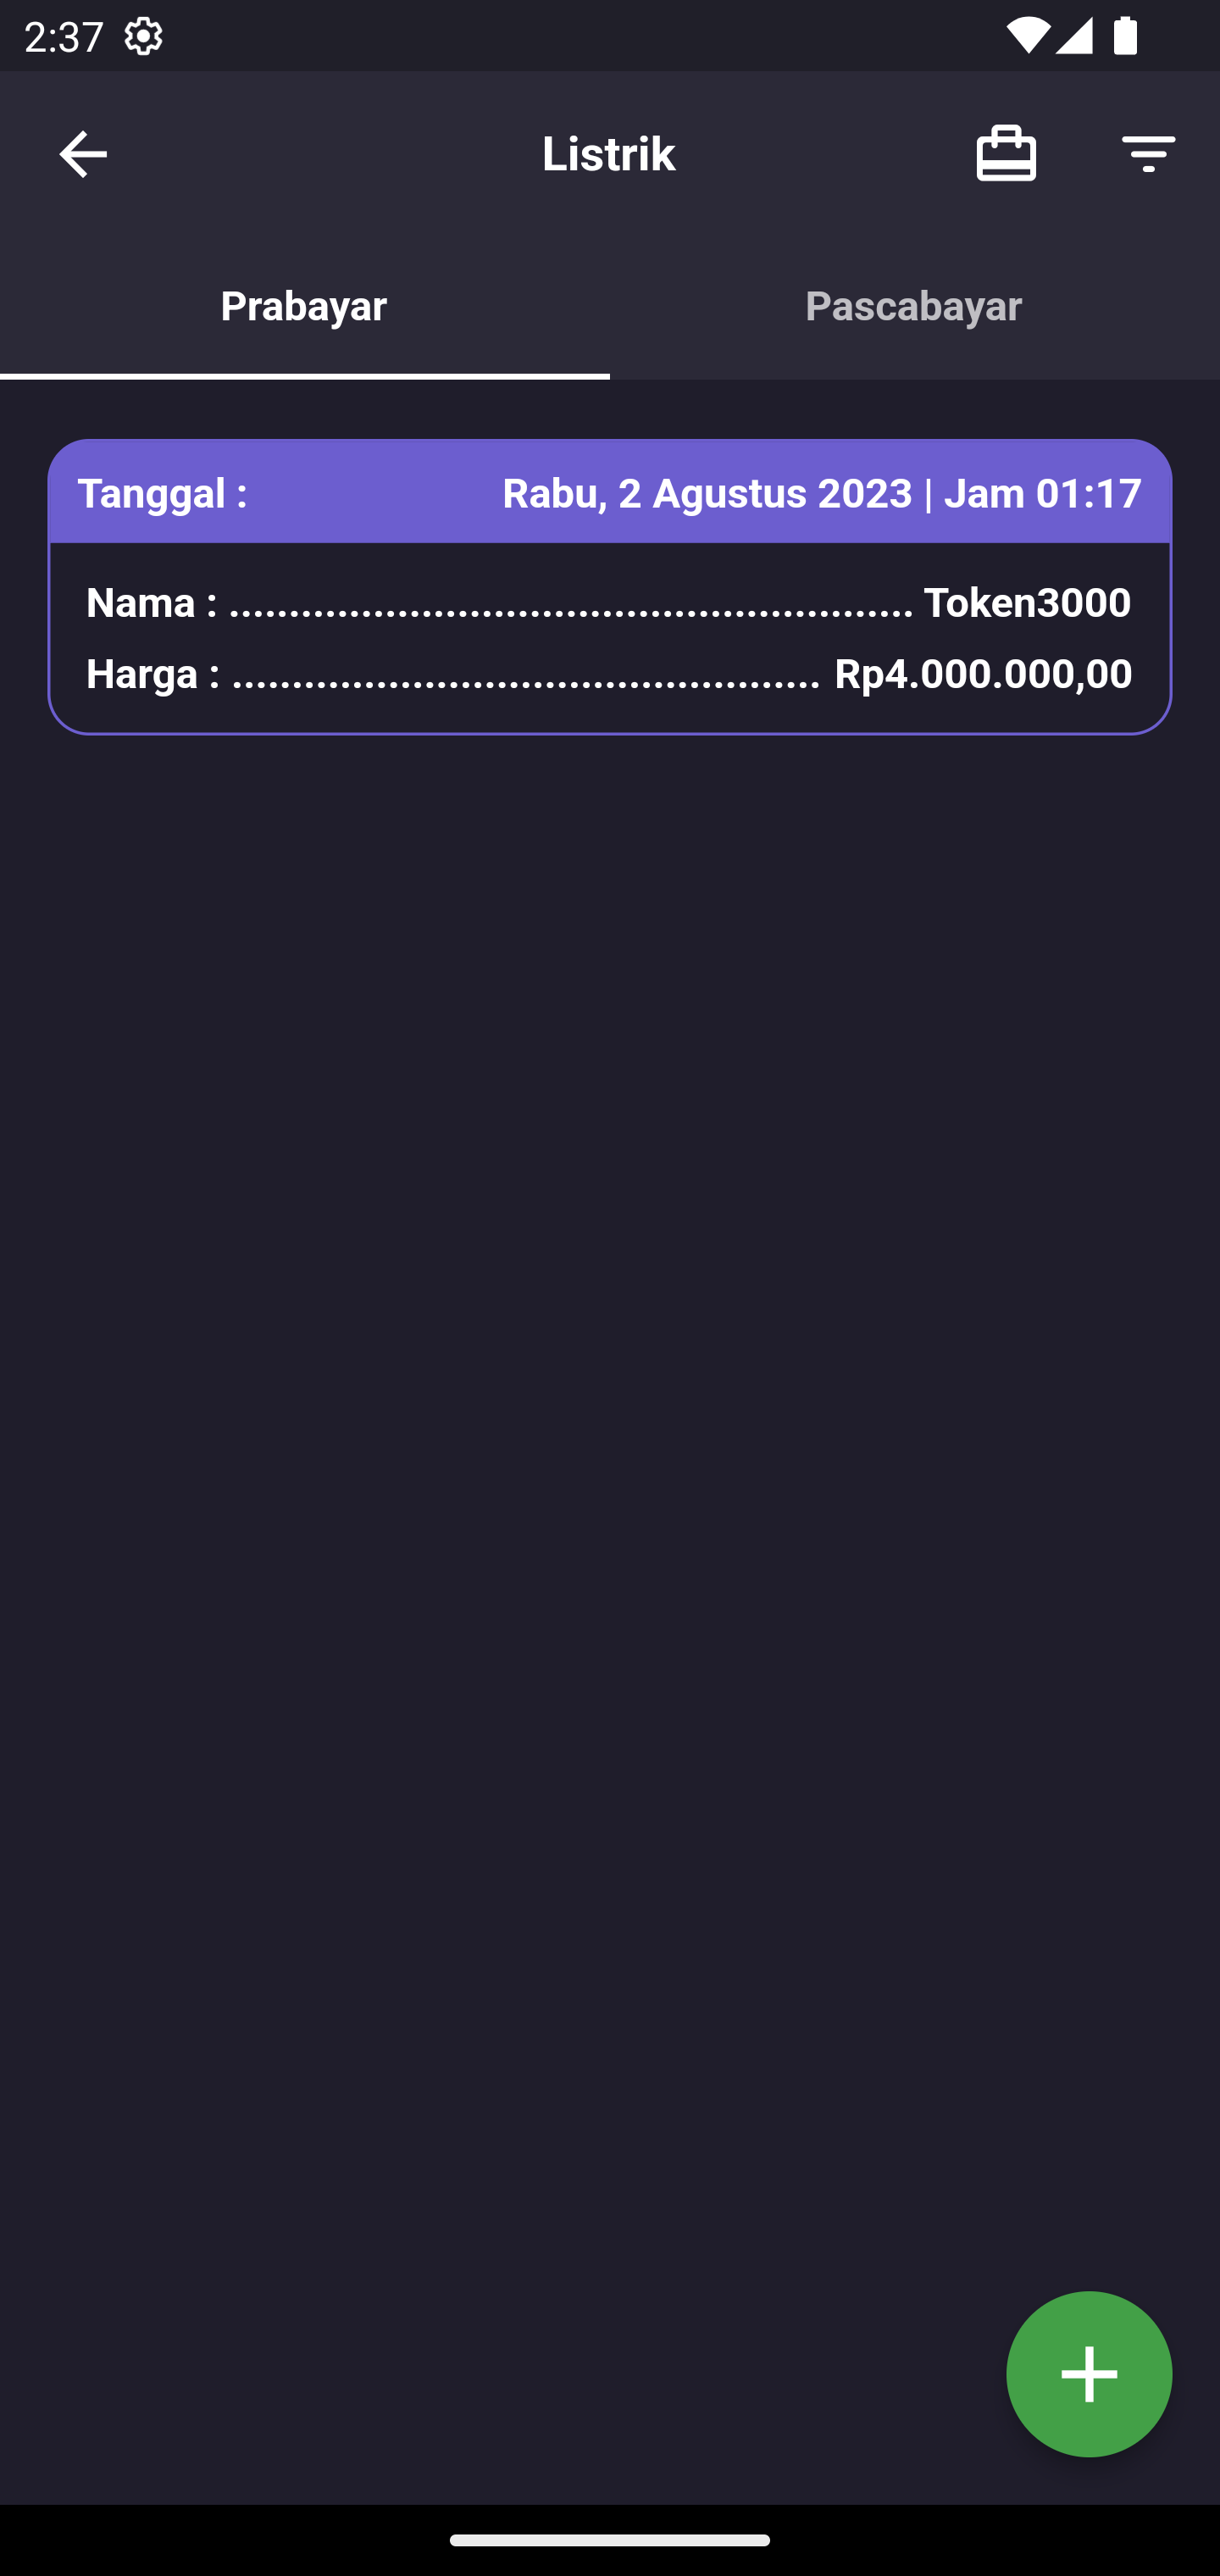
\includegraphics[width=\linewidth]{gambar/sprint4/el_1.png}
						\caption{Halaman Inventaris Listrik}
					\endminipage\hfill
					\minipage{0.32\textwidth}
						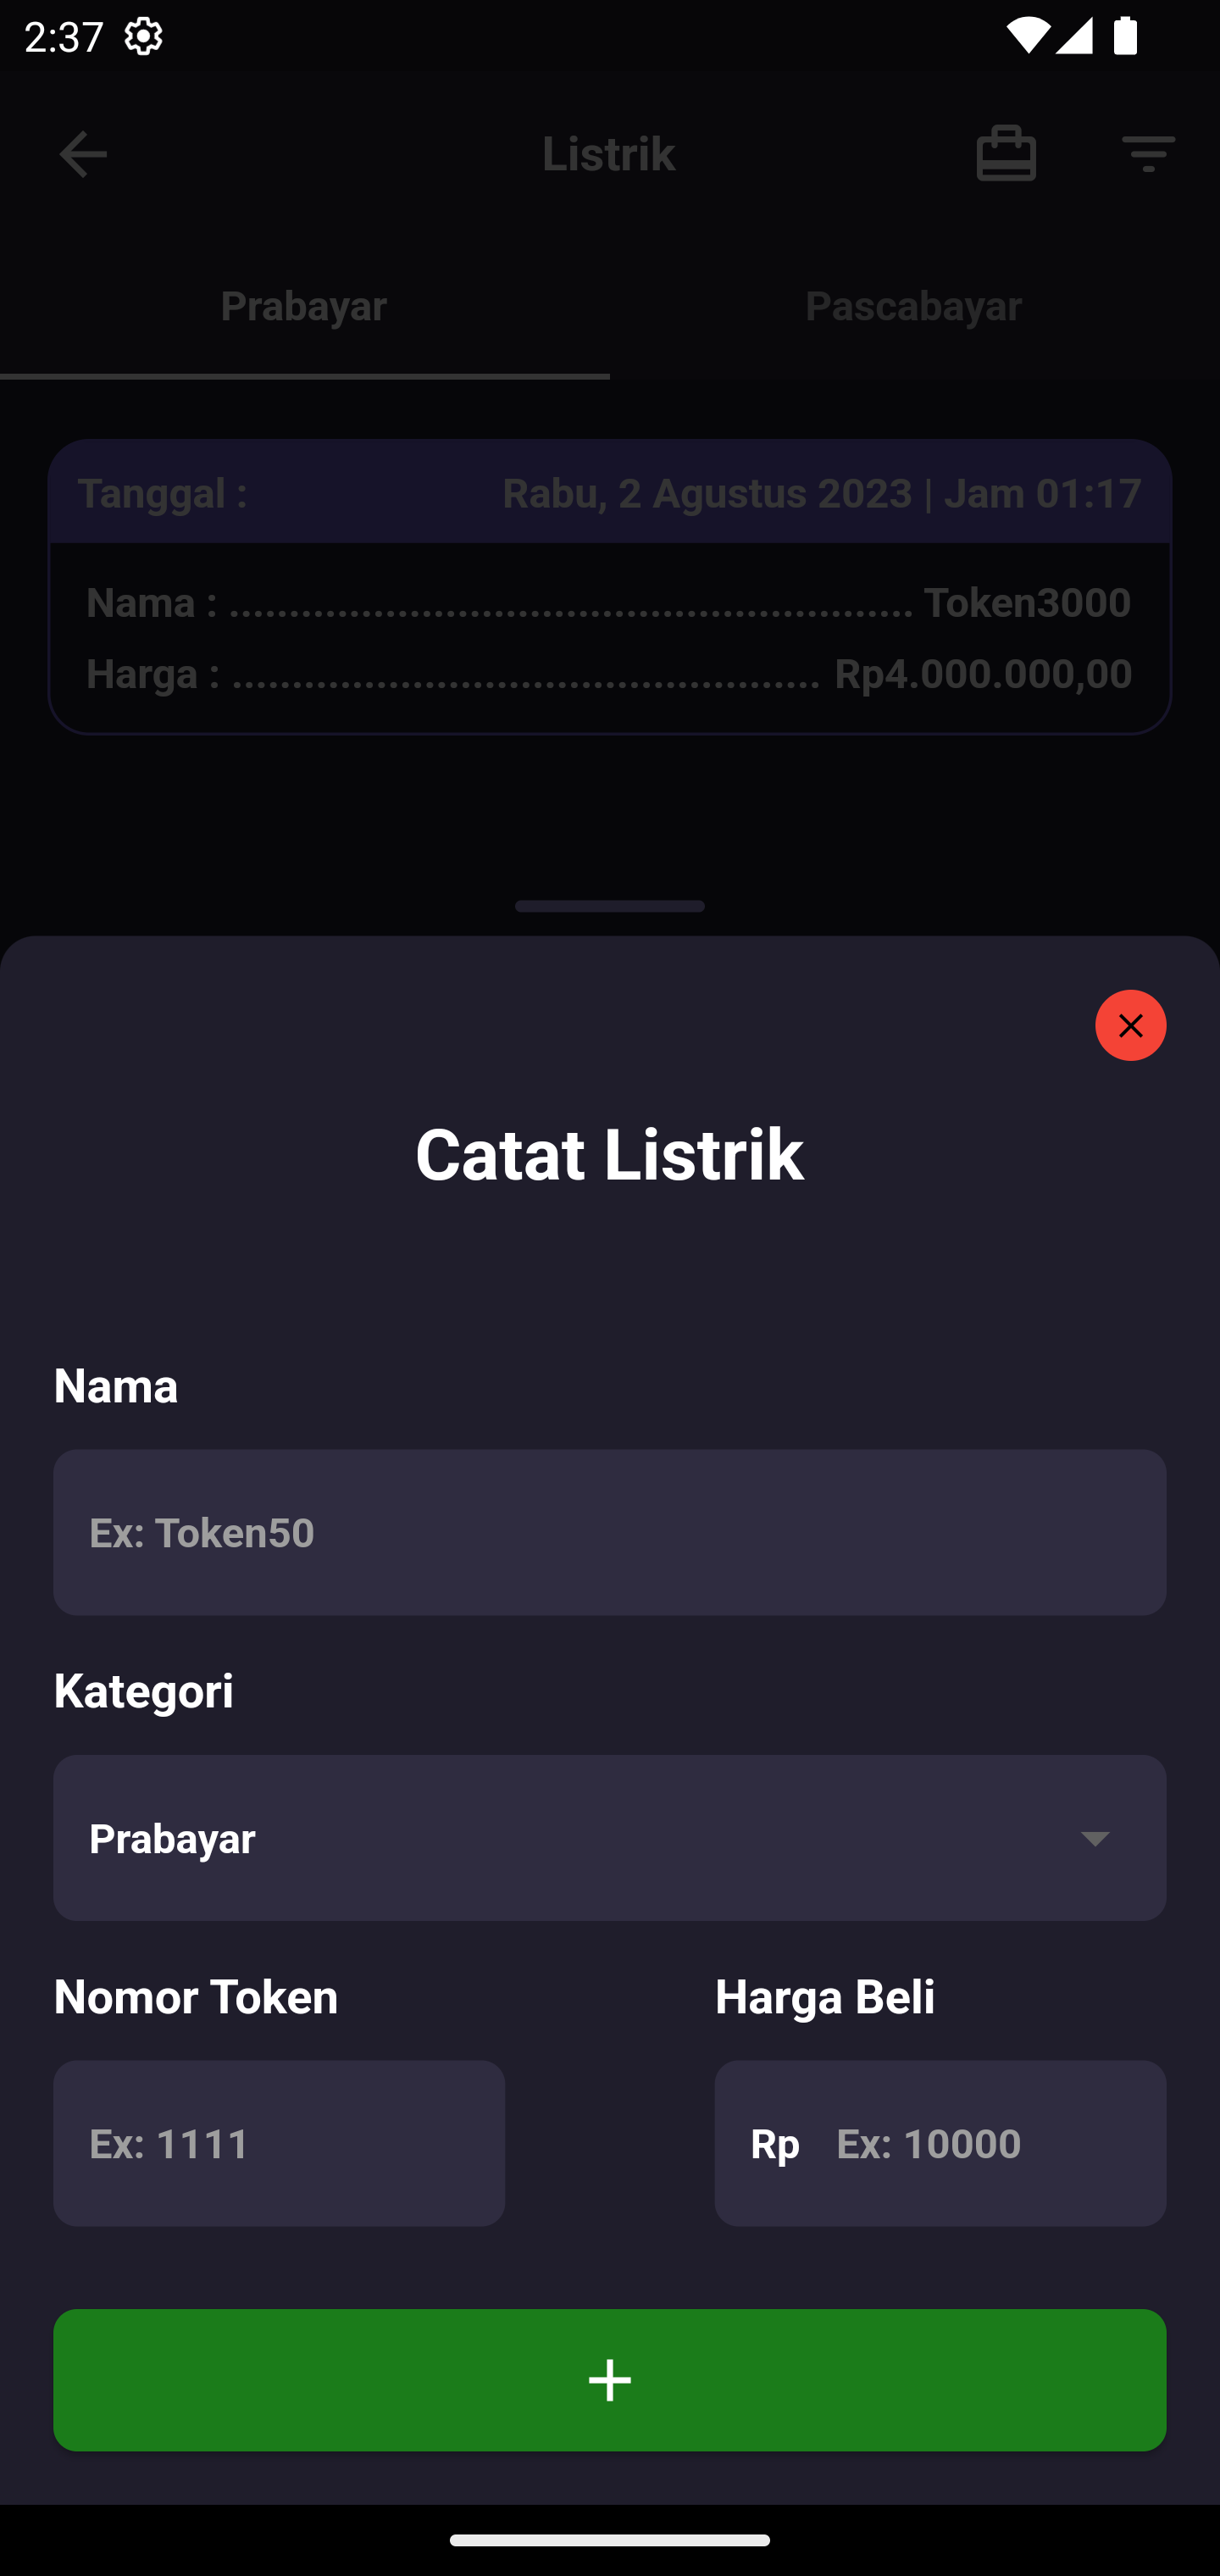
\includegraphics[width=\linewidth]{gambar/sprint4/el_2.png}
						\caption{Halaman Input Inventaris Listrik}
					\endminipage\hfill
					\minipage{0.32\textwidth}
						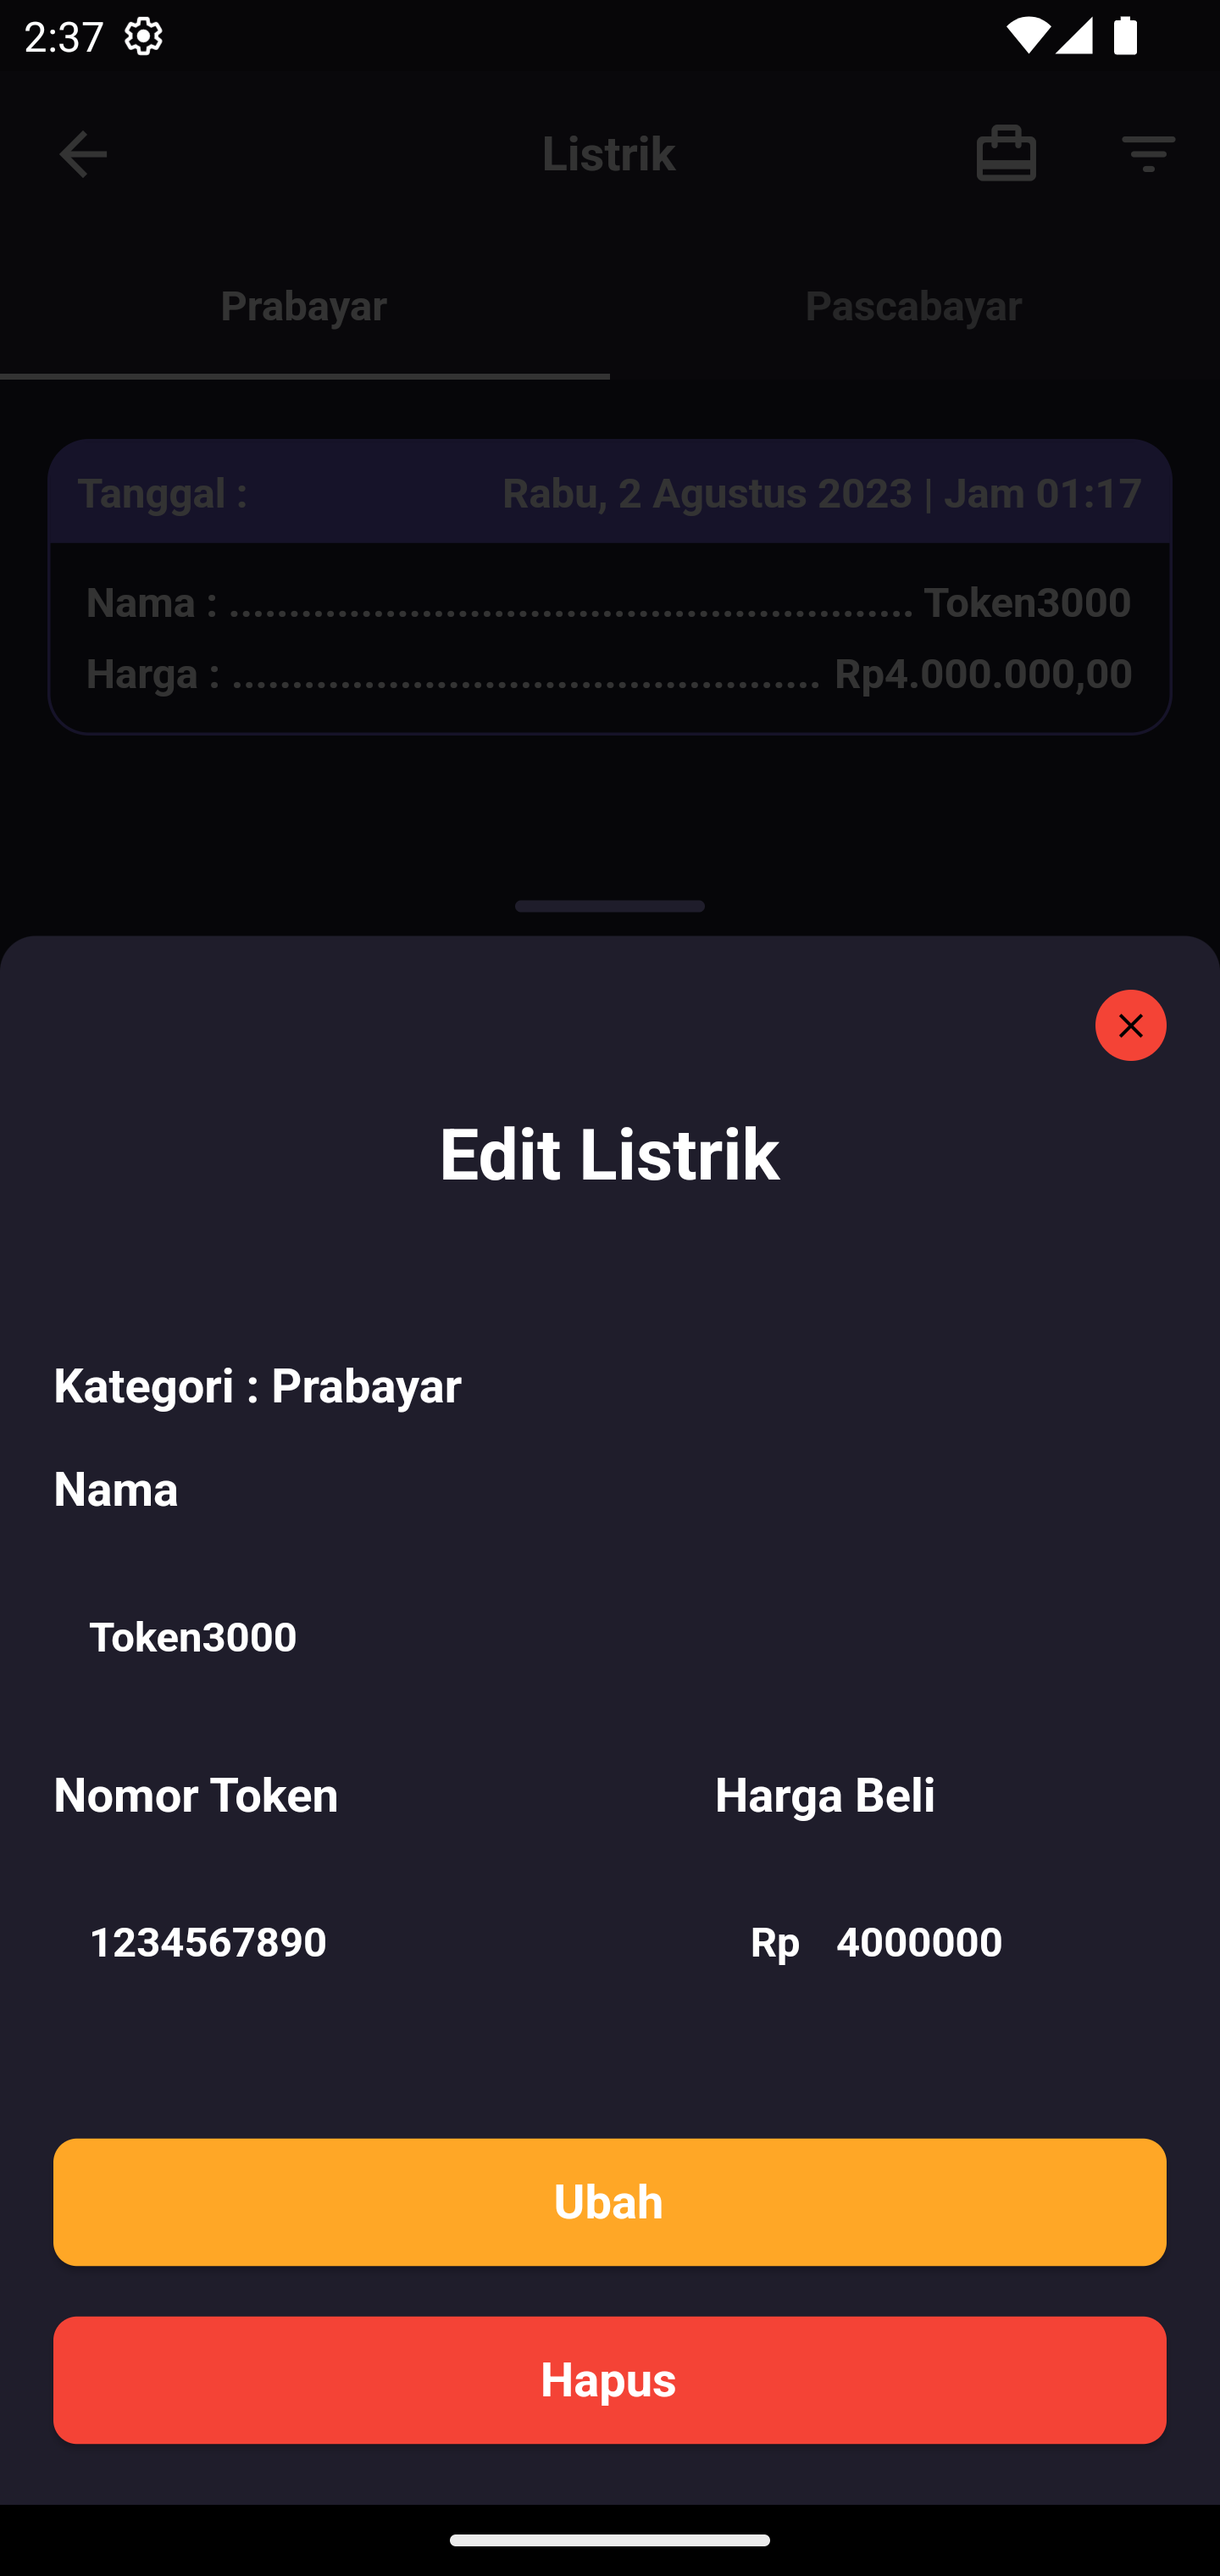
\includegraphics[width=\linewidth]{gambar/sprint4/el_3.png}
						\caption{Halaman Detail Inventaris Listrik}
					\endminipage\hfill
				\end{figure}

				Pada tampilan tersebut, dapat dilihat bahwa terdapat filter listrik yang berupa pakan prabayar dan pascabayar, masing-masing memiliki input form yang berbeda. Serta di bagian center terdapat bagian yang menampilkan list dari inventaris listrik yang sudah terdaftar.

				Dibagian Catat Listrik, terdapat form isian yang harus dilengkapi jika ingin mencatat inventaris listrik. Kemudian, pada halaman Edit Listrik memiliki layout yang kurang lebih sama seperti Catat Listrik namun fungsi yang digunakan berbeda.

				\end{itemize}
		\end{enumerate}
		
		\item Design route dan penerapan pada Flutter untuk inventaris aset (dalam bentuk RESTful API)
		
		\begin{enumerate}
			\item Design Sample Route
			
			Berikut merupakan sample route yang sudah dibuat untuk inventaris aset.

			\begin{figure}[H]
				\centering
				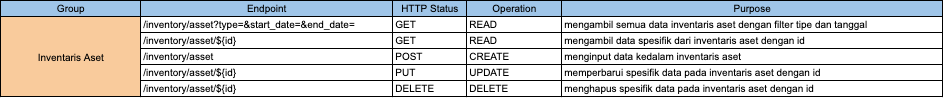
\includegraphics[width=1\textwidth]{gambar/sprint4/samle_route_aset.png}
				\caption{Sample Route Inventaris Aset}
			\end{figure}

			\item Model Backend
 			
			Berdasarkan sample route tersebut, dapat dibuat model dan class HTTP method pada backend. Berikut model serta class untuk inventaris aset :

			\begin{itemize}
				\item Model Inventaris Aset
				
				\begin{lstlisting}
					class AssetInventory(db.Document):
						id_int = db.SequenceField(required=True)
						farm_id = db.ReferenceField(Farm, required=True)
						asset_category = db.StringField(required=True)
						name = db.StringField(required=True)
						description = db.StringField(required=True)
						amount = db.IntField(required=True)
						price = db.IntField(required=True)
						image = db.StringField(required=True)
						created_at = db.DateTimeField(default=datetime.datetime.now)
						updated_at = db.DateTimeField(default=datetime.datetime.now)
				\end{lstlisting}

				% Pada model tersebut, terdapat beberapa \textit{key} seperti feed\_name\_id yang digunakan untuk mereferensikan kepada tabel FeedName, farm\_id untuk mereferensikan kepada tabel Farm, id\_int untuk 

				\end{itemize}

			\item Fungsi-fungsi HTTP Method
			
			\begin{itemize}
				\item Mengambil semua data inventaris aset (HTTP Method - GET)
				
				\begin{lstlisting}
					class AssetInventoriesApi(Resource):
						@jwt_required()
						def get(self):
							try:
								current_user = get_jwt_identity()
								farm = str(current_user['farm_id'])
								farm_id = ObjectId(farm)
					
								type = request.args.get('type') if request.args.get('type') else ""
								start_date = datetime.datetime.strptime(request.args.get('start_date'), '%Y-%m-%d') if request.args.get('start_date') else datetime.datetime.strptime("2023-01-01", '%Y-%m-%d')
								end_date = datetime.datetime.strptime(request.args.get('end_date'), '%Y-%m-%d') + datetime.timedelta(days=1) if request.args.get('end_date') else datetime.datetime.strptime("2030-01-01", '%Y-%m-%d')
					
								pipeline = [
									{"$sort": {"id_int": 1}},
									{
										'$match': {
											"farm_id": farm_id,
											'asset_category': {
												'$regex': type,
												'$options': 'i'
											},
											'created_at': {
												'$gte': start_date,
												'$lte': end_date,
											}
										}
									},
								]
							
								testing = AssetInventory.objects.aggregate(pipeline)
								temp = list(testing)
								response = json.dumps({
									'status': 'success',
									'data': temp,
								}, default=str)
								return Response(response, mimetype="application/json", status=200)
							except Exception as e:
								response = {"message": e}
								response = json.dumps(response, default=str)
								return Response(response, mimetype="application/json", status=400)
				\end{lstlisting}

				\item Mengambil spesifik data inventaris aset (HTTP Method - GET)
				
				\begin{lstlisting}
					class AssetInventoryApi(Resource):
						def get(self, id):
							try:
								pipeline = {"$match": {"id_int": int(id)}},
								testing = AssetInventory.objects.aggregate(pipeline)
								temp = list(testing)
								if len(temp) == 0:
									res = {"message": 'no data found'}
									response = json.dumps(res, default=str)
									return Response(response, mimetype="application/json", status=200)
								response = json.dumps({
									'status': 'success',
									'data': temp[0],
								}, default=str)
								return Response(response, mimetype="application/json", status=200)
							except Exception as e:
								response = {"message": e}
								response = json.dumps(response, default=str)
								return Response(response, mimetype="application/json", status=400)
				\end{lstlisting}

				\item Menambahkan data inventaris aset (HTTP Method - POST)
				
				\begin{lstlisting}
					class AssetInventoriesApi(Resource):
						@jwt_required()
						def post(self):
							try:
								current_user = get_jwt_identity()
								farm = str(current_user['farm_id'])
								body = {
									"farm_id": farm,
									"asset_category": request.form.get('asset_category', None),
									"name": request.form.get('name', None),
									"description": request.form.get('description', None),
									"amount": request.form.get('amount', None),
									"price": request.form.get('price', None),
									"image": request.form.get('image', None),
								}
								inventory = AssetInventory(**body).save()
								id = inventory.id
								res = {"message": "success add asset to inventory", "id": id, "data": body}
								response = json.dumps(res, default=str)
								return Response(response, mimetype="application/json", status=200)
							except Exception as e:
								response = {"message": str(e)}
								response = json.dumps(response, default=str)
								return Response(response, mimetype="application/json", status=400)
				\end{lstlisting}

				\item Memperbarui spesifik data inventaris aset (HTTP Method - PUT)
				
				\begin{lstlisting}
					class AssetInventoryApi(Resource):
						def put(self, id):
							try:
								body = {       
									"id_int": int(id),
									"asset_category": request.form.get('asset_category', None),
									"name": request.form.get('name', None),
									"description": request.form.get('description', None),
									"amount": request.form.get('amount', None),
									"price": request.form.get('price', None),
									"image": request.form.get('image', None),
								}
								inventory = AssetInventory.objects.get(id_int = int(id)).update(**body)
								response = {"message": "success update asset inventory", "data": body}
								response = json.dumps(response, default=str)
								return Response(response, mimetype="application/json", status=200)
							except Exception as e:
								response = {"message": str(e)}
								response = json.dumps(response, default=str)
								return Response(response, mimetype="application/json", status=400)
				\end{lstlisting}

				\item Menghapus spesifik data inventaris aset (HTTP Method - DELETE)
				
				\begin{lstlisting}
					class AssetInventoryApi(Resource):
						def delete(self, id):
							try:
								inventory = AssetInventory.objects.get(id_int = int(id)).delete()
								response = {"message": "success delete asset inventory"}
								response = json.dumps(response, default=str)
								return Response(response, mimetype="application/json", status=200)
							except Exception as e:
								response = {"message": str(e)}
								response = json.dumps(response, default=str)
								return Response(response, mimetype="application/json", status=400)
				\end{lstlisting}
			\end{itemize}

			\item Controller HTTP pada Flutter
			
			\begin{itemize}
				\item Mengambil semua data inventaris aset (HTTP Method - GET)
				
				\begin{lstlisting}
					Future getAllData(
						String type, String first, String last, Function() doAfter) async {
					  assetList.value.data!.clear();
					  isLoadingPage.value = true;
				  
					  SharedPreferences prefs = await SharedPreferences.getInstance();
					  String token = prefs.getString('token').toString();
					  var headers = {'Authorization': 'Bearer $token'};
				  
					  final response = await http.get(
						Uri.parse('${Urls.invAsset}?type=$type&start_date=$first&end_date=$last'),
						headers: headers,
					  );
				  
					  try {
						if (response.statusCode == 200) {
						  InventarisAssetModel res =
							  InventarisAssetModel.fromJson(jsonDecode(response.body));
				  
						  assetList.value = res;
				  
						  doAfter();
						}
					  } catch (e) {
						throw Exception(e);
					  }
					  isLoadingPage.value = false;
					}
				\end{lstlisting}

				\item Mengambil spesifik data inventaris aset (HTTP Method - GET)
				
				\begin{lstlisting}
					Future getDataByID(int id, Function() doAfter) async {
						isLoadingDetail.value = true;

						final response = await http.get(Uri.parse('${Urls.invAsset}/$id'));

						try {
						if (response.statusCode == 200) {
							DetailInventarisAssetModel res =
								DetailInventarisAssetModel.fromJson(jsonDecode(response.body));

							assetCategory.value = res.data!.assetCategory!.toString();
							name.text = res.data!.name.toString();
							desc.text = res.data!.description.toString() == ''
								? '-'
								: res.data!.description.toString();
							price.text = res.data!.price.toString();
							amount.text = res.data!.amount.toString();
							image.value = res.data!.image.toString();
						}
						doAfter();
						} catch (e) {
						throw Exception(e);
						}
						isLoadingDetail.value = false;
					}
				\end{lstlisting}

				\item Menambahkan data inventaris aset (HTTP Method - POST)
				
				\begin{lstlisting}
					Future postData(Function() doAfter) async {
						var map = <String, dynamic>{};
					
						SharedPreferences prefs = await SharedPreferences.getInstance();
						String token = prefs.getString('token').toString();
						var headers = {'Authorization': 'Bearer $token'};
						map['asset_category'] = assetCategory.value;
						map['name'] = name.text;
						map['description'] = desc.text;
						map['price'] = price.text;
						map['amount'] = amount.text;
						map['image'] = image.value;
					
						isLoadingPost.value = true;
					
						try {
						  final res = await http.post(
							Uri.parse(Urls.invAsset),
							body: map,
							headers: headers,
						  );
						  inspect(res);
						  doAfter();
						} catch (e) {
						  throw Exception(e);
						}
						isLoadingPost.value = false;
					  }
				\end{lstlisting}

				\item Memperbarui spesifik data inventaris aset (HTTP Method - PUT)
				
				\begin{lstlisting}
					Future updateData(int id, Function() doAfter) async {
						var map = <String, dynamic>{};

						map['asset_category'] = assetCategory.value;
						map['name'] = name.text;
						map['description'] = desc.text == '' ? '-' : desc.text;
						map['price'] = price.text;
						map['amount'] = amount.text;
						map['image'] = image.value;

						isLoadingPost.value = true;

						try {
						// inspect(map);
						final res = await http.put(
							Uri.parse('${Urls.invAsset}/$id'),
							body: map,
						);
						// inspect(res);
						doAfter();
						} catch (e) {
						throw Exception(e);
						}
						isLoadingPost.value = false;
					}
				\end{lstlisting}

				\item Menghapus spesifik data inventaris aset (HTTP Method - DELETE)
				
				\begin{lstlisting}
					Future deleteData(int id, Function() doAfter) async {
						isLoadingDelete.value = true;
						try {
						await http.delete(
							Uri.parse(
							'${Urls.invAsset}/$id',
							),
							headers: {
							'Content-Type': 'application/json; charset=UTF-8',
							},
						);
						doAfter();
						} catch (e) {
						throw Exception(e);
						}
						isLoadingDelete.value = false;
					}
				\end{lstlisting}
			\end{itemize}

			\item Tampilan pada Flutter
			
			\begin{itemize}
				\item Halaman Inventaris Aset, Input Aset, dan Detail Aset
				
				\begin{figure}[H]
					\minipage{0.32\textwidth}
						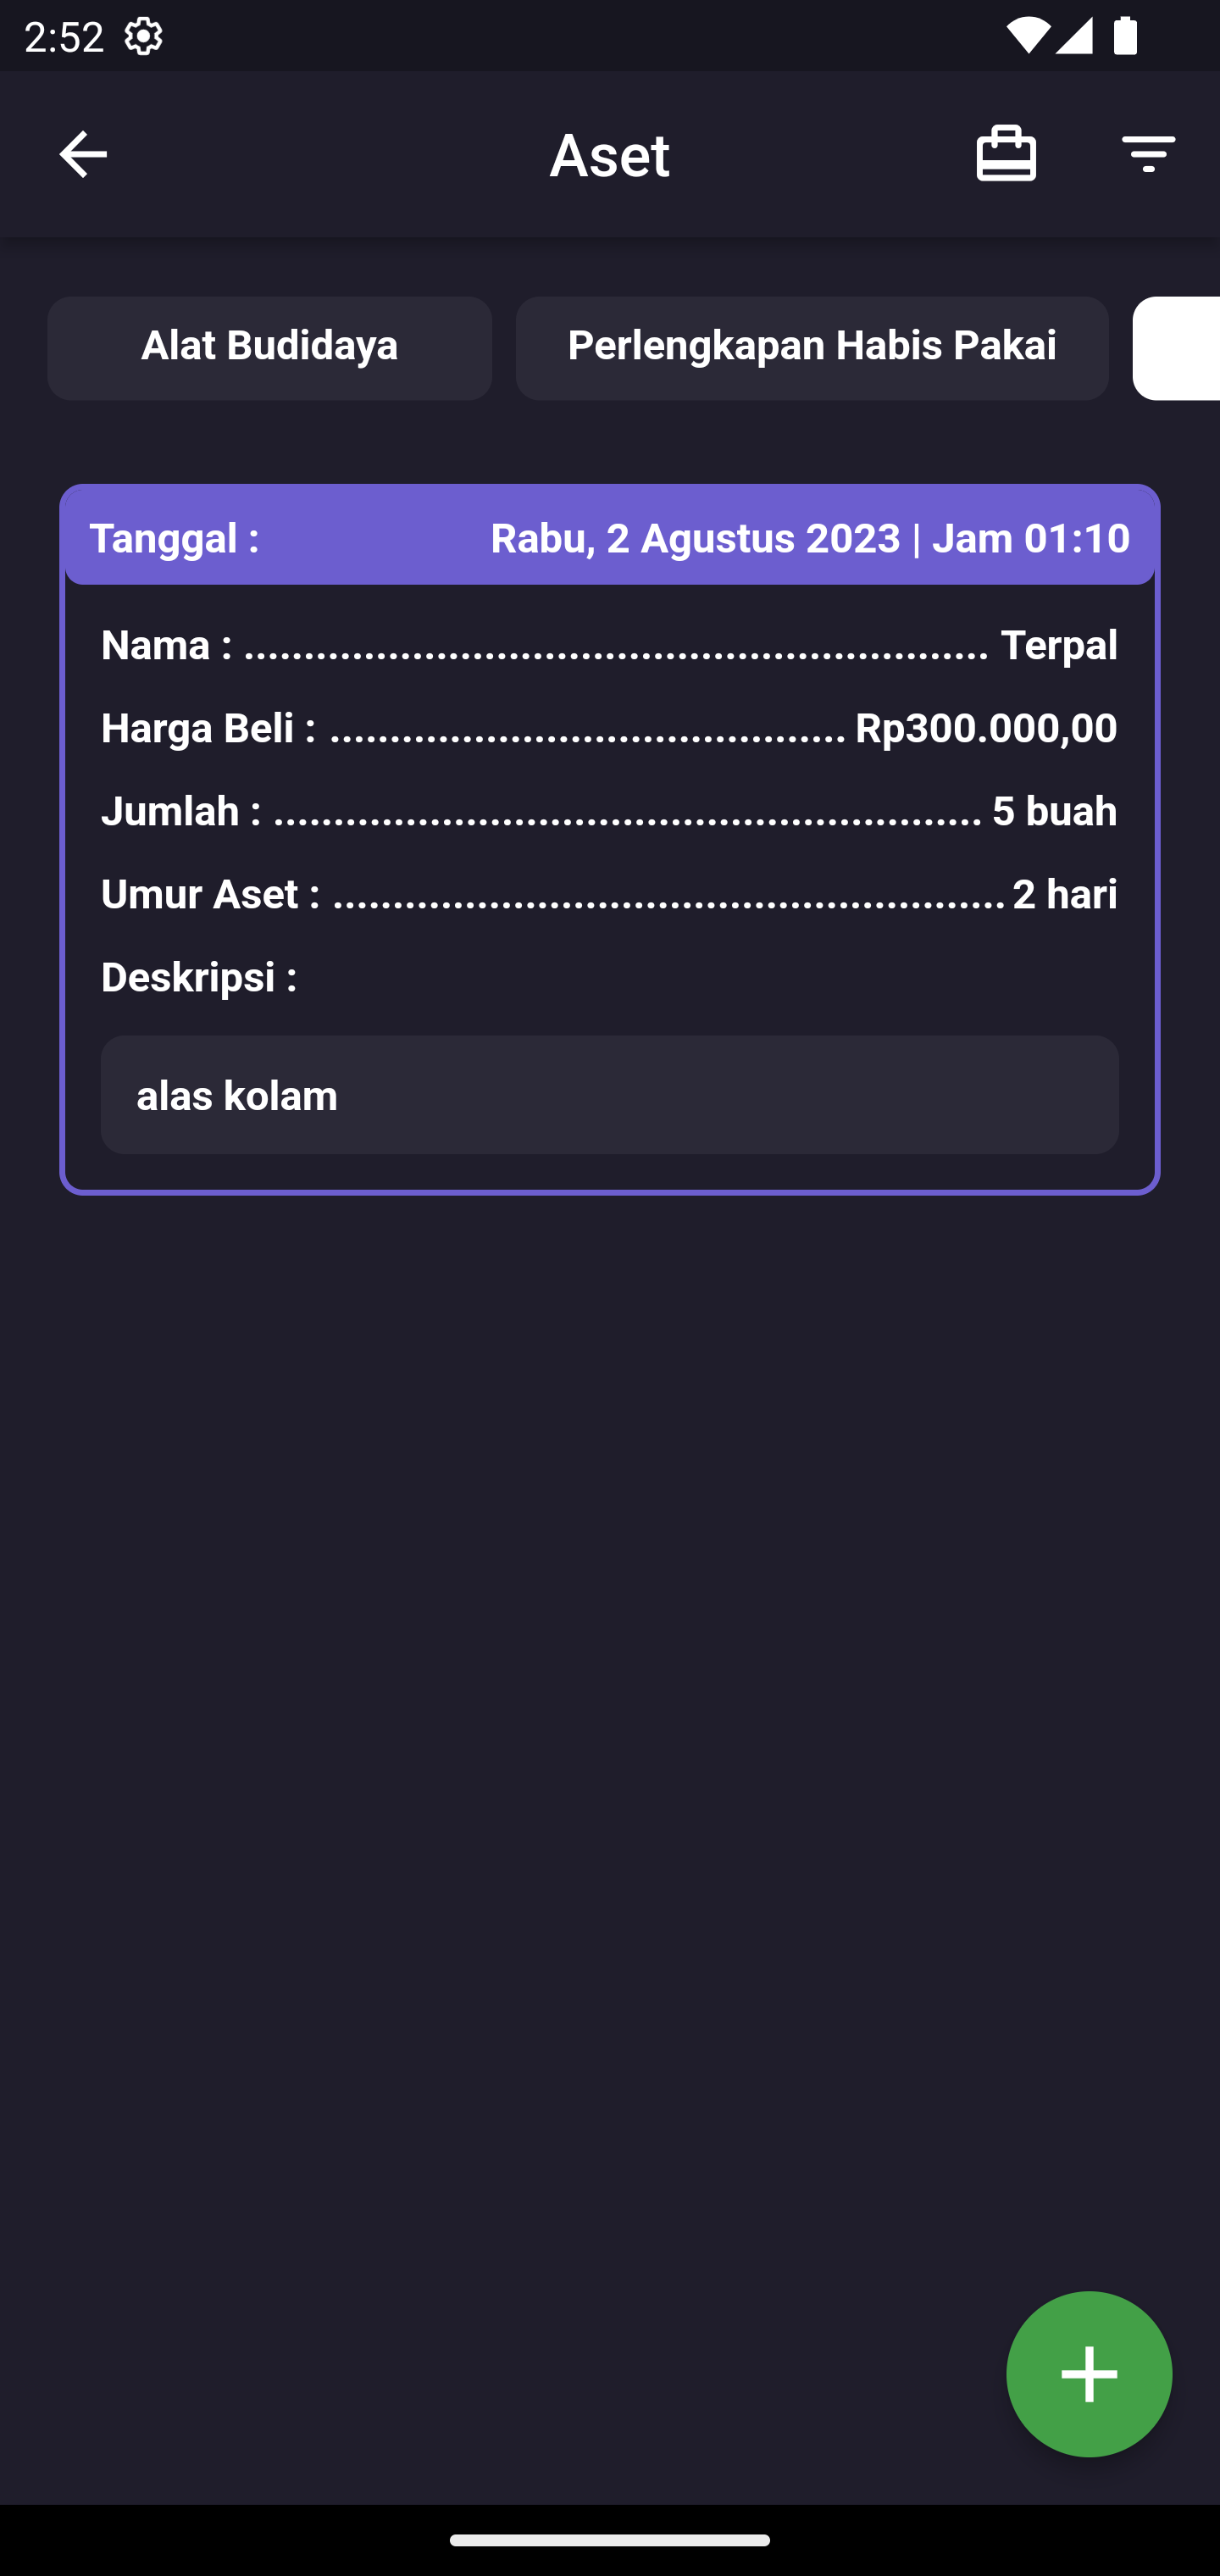
\includegraphics[width=\linewidth]{gambar/sprint4/as_1.png}
						\caption{Halaman Inventaris Aset}
					\endminipage\hfill
					\minipage{0.32\textwidth}
						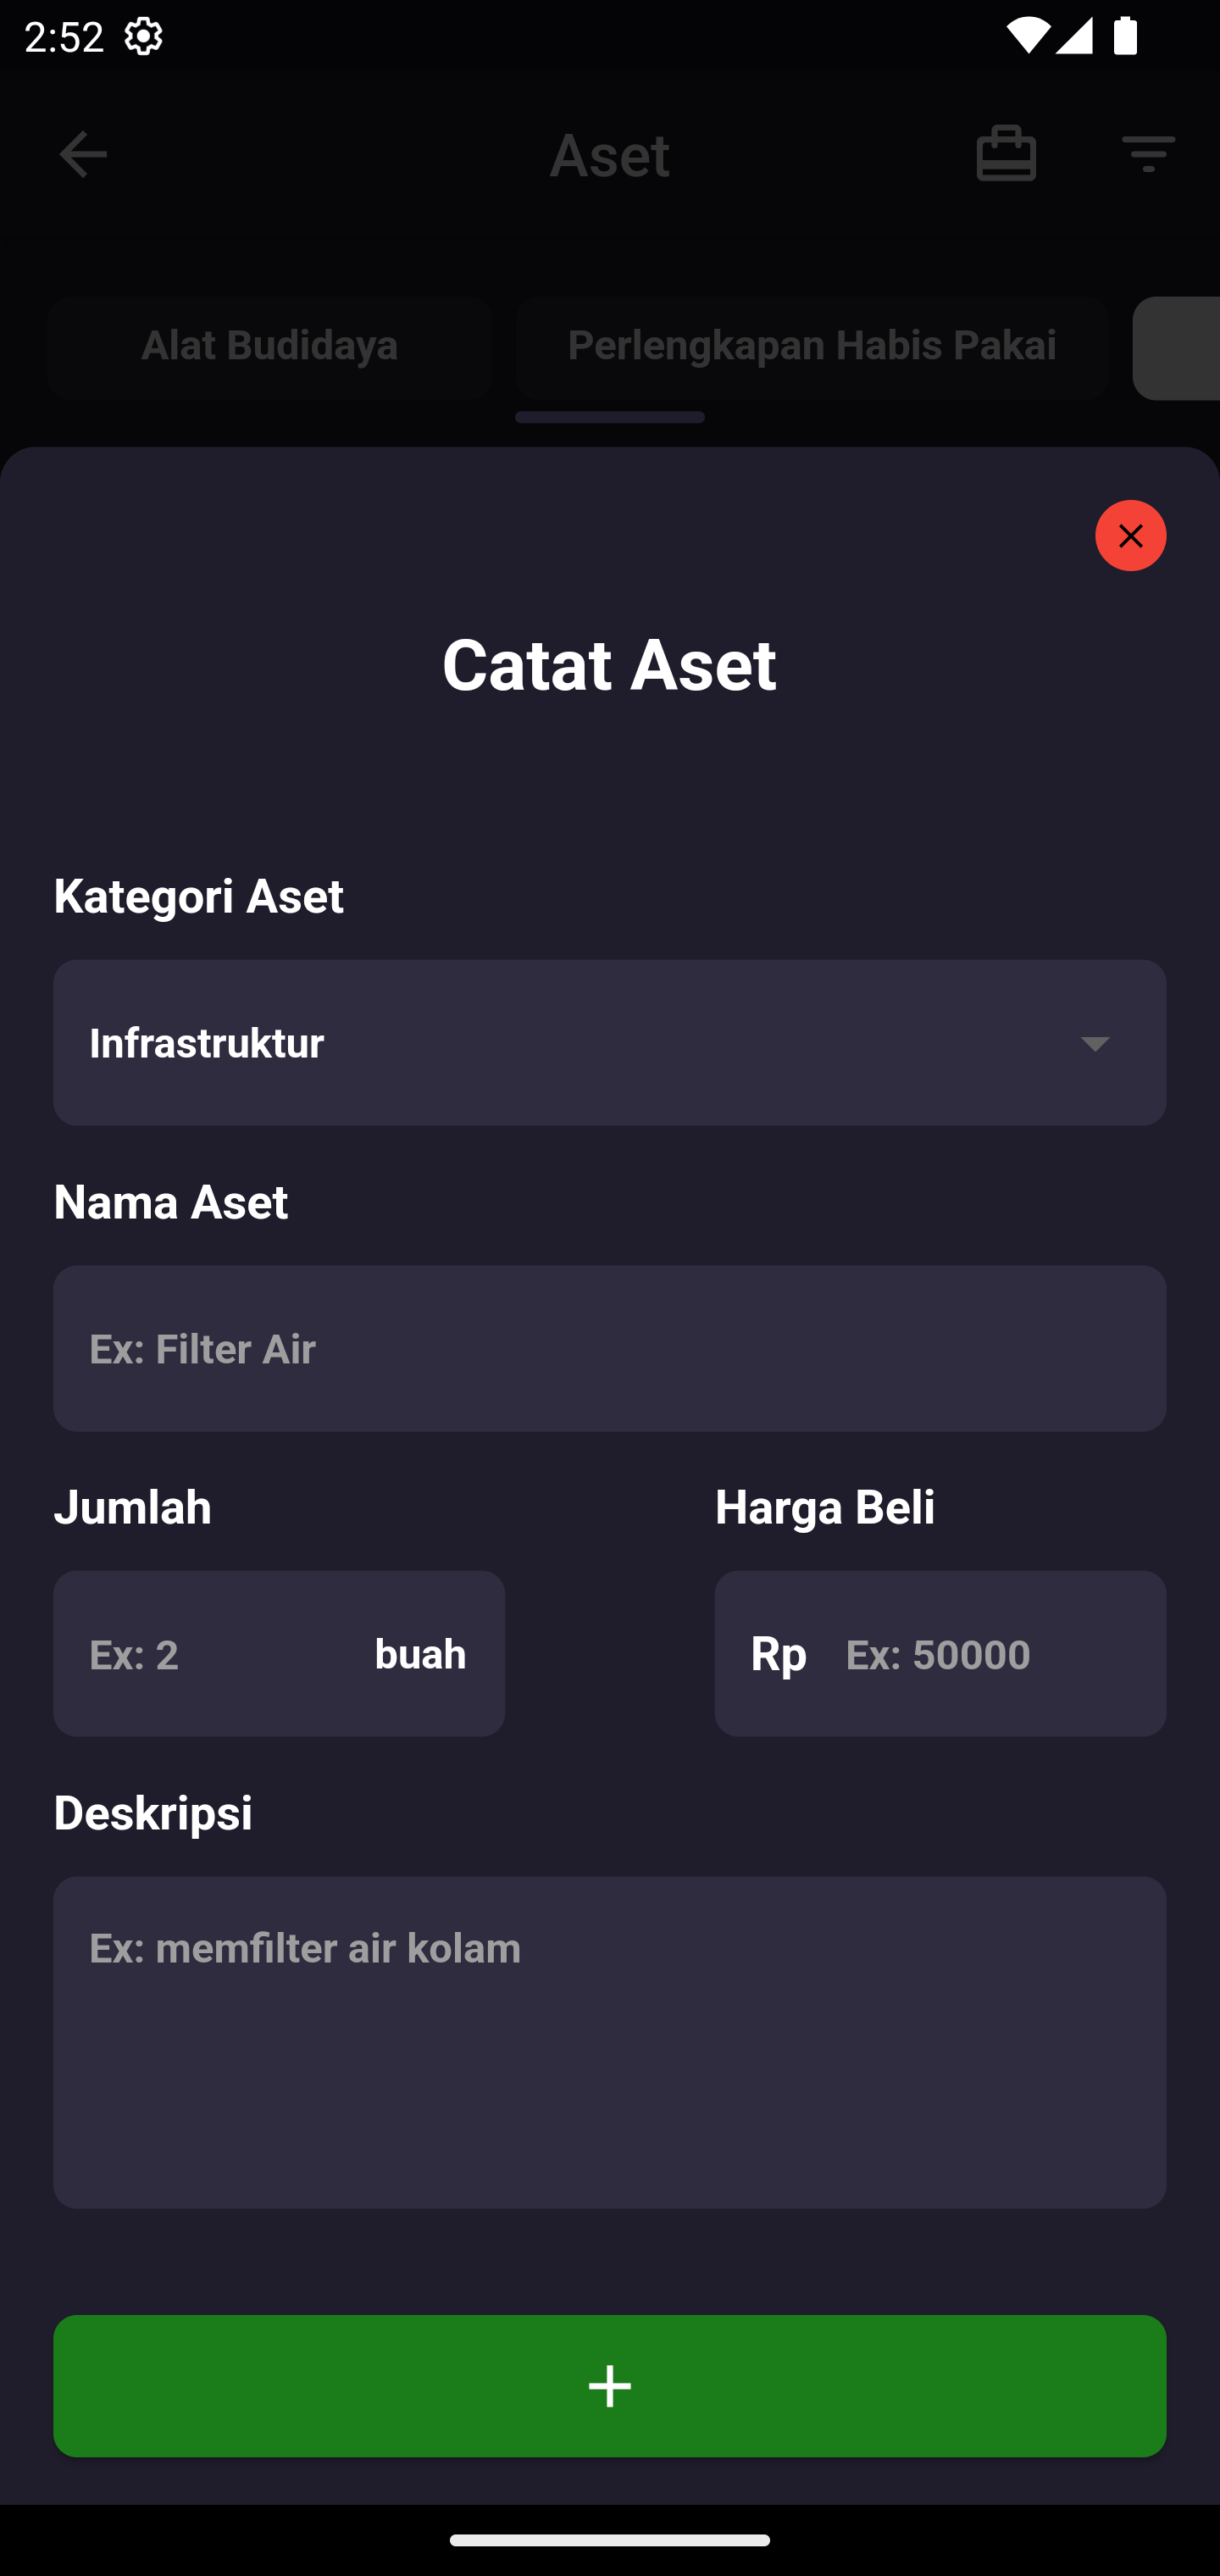
\includegraphics[width=\linewidth]{gambar/sprint4/as_2.png}
						\caption{Halaman Input Inventaris Aset}
					\endminipage\hfill
					\minipage{0.32\textwidth}
						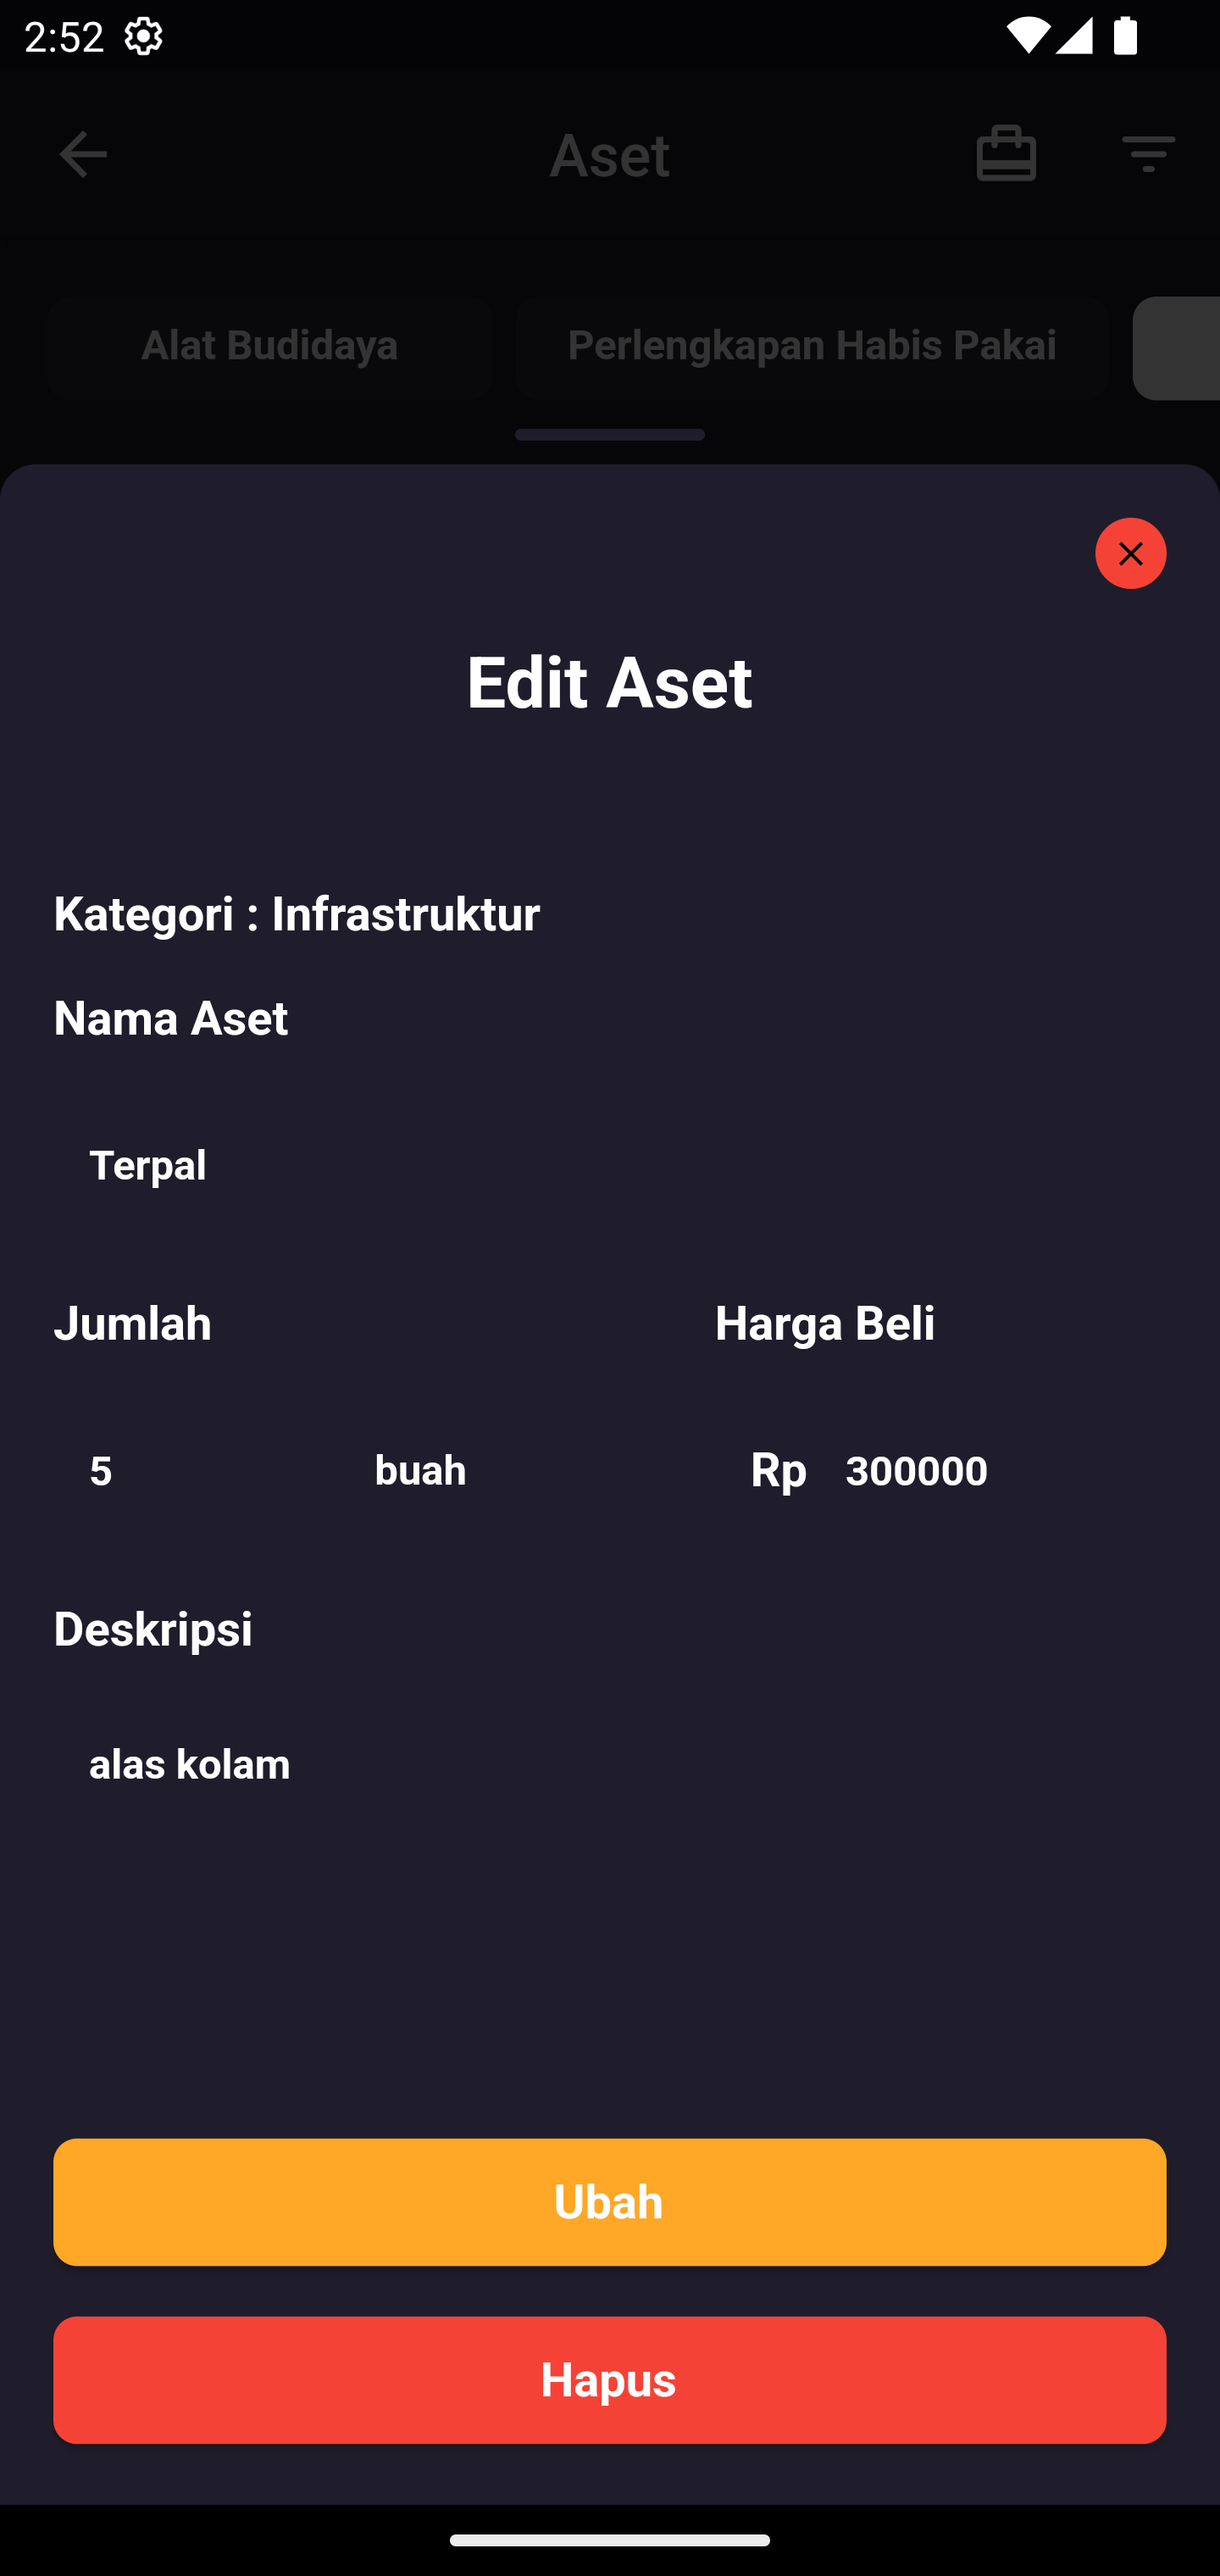
\includegraphics[width=\linewidth]{gambar/sprint4/as_3.png}
						\caption{Halaman Detail Inventaris Aset}
					\endminipage\hfill
				\end{figure}

				Pada tampilan tersebut, dapat dilihat bahwa terdapat filter pakan yang berupa aset alat budidaya, aset perlengkapan habis pakai, aset infrastruktur, dan lainnya. Serta di bagian center terdapat bagian yang menampilkan list dari inventaris aset yang sudah terdaftar.

				Dibagian Catat Aset, terdapat form isian yang harus dilengkapi jika ingin mencatat Aset. Kemudian, pada halaman Edit Aset memiliki layout yang kurang lebih sama seperti Catat Aset namun fungsi yang digunakan berbeda.
		
			\end{itemize}
		\end{enumerate}
		
		\item Design route dan penerapan pada Flutter untuk riwayat pemakaian pakan (dalam bentuk RESTful API) 
		
		\begin{enumerate}
			\item Design Sample Route
			
			Berikut merupakan sample route yang sudah dibuat untuk riwayat pemakaian pakan.

			\begin{figure}[H]
				\centering
				\includegraphics[width=1.1\textwidth]{gambar/sprint4/pakan_hs_route.png}
				\caption{Sample Route Riwayat Pemakaian Pakan}
			\end{figure}

			\item Model Backend
 			
			Berdasarkan sample route tersebut, dapat dibuat model dan class HTTP method pada backend. Berikut model serta class untuk riwayat pemakaian pakan :

			\begin{itemize}
				\item Model Riwayat Pemakaian Pakan
				
				\begin{lstlisting}
					class FeedUsed(db.Document):
						fish_feed_id = db.ReferenceField(FeedInventory, required=True)
						farm_id = db.ReferenceField(Farm, required=True)
						original_amount = db.FloatField(required=True)
						usage = db.FloatField(required=True)
						pond = db.StringField(required=True)
						created_at = db.DateTimeField(default=datetime.datetime.now)
						updated_at = db.DateTimeField(default=datetime.datetime.now)
				\end{lstlisting}

				% Pada model tersebut, terdapat beberapa \textit{key} seperti feed\_name\_id yang digunakan untuk mereferensikan kepada tabel FeedName, farm\_id untuk mereferensikan kepada tabel Farm, id\_int untuk 

				\end{itemize}

			\item Fungsi-fungsi HTTP Method
			
			\begin{itemize}
				\item Mengambil semua data riwayat pemakaian pakan (HTTP Method - GET)
				
				\begin{lstlisting}
					class FeedFishHistoryApi(Resource):
						@jwt_required()

						def get(self):
							try:
								current_user = get_jwt_identity()
								farm = str(current_user['farm_id'])
								farm_id = ObjectId(farm)

								start_date = datetime.datetime.strptime(request.args.get('start_date'), '%Y-%m-%d') if request.args.get('start_date') else datetime.datetime.strptime("2023-01-01", '%Y-%m-%d')
								end_date = datetime.datetime.strptime(request.args.get('end_date'), '%Y-%m-%d') + datetime.timedelta(days=1) if request.args.get('end_date') else datetime.datetime.strptime("2030-01-01", '%Y-%m-%d')
								name = request.args.get('name') if request.args.get('name') else ""
								pond_name = request.args.get('pond_name') if request.args.get('pond_name') else ""

								pipeline = [
									{
										'$match': {
											'created_at': {
												'$gte': start_date,
												'$lte': end_date,
											}
										}
									},
									{
										'$match': {
											"farm_id": farm_id,
											'pond': {
												'$regex': pond_name,
												'$options': 'i'
											}
										}
									},
									{"$sort": {"fish_feed_id": 1}},
									{'$lookup': {
										'from': 'feed_inventory',
										'let': {"fishfeedid": "$fish_feed_id"},
										'pipeline': [
											{'$match': {'$expr': {'$eq': ['$_id', '$$fishfeedid']}}},
											{
												'$match': {
													'brand_name': {
														'$regex': name,
														'$options': 'i'
													}
												}
											},
											{"$project": {
												"_id": 1,
												"id_int": 1,
												"feed_category": 1,
												"brand_name": 1,
												"price": 1,
												"amount": 1,
												"created_at": 1,
											}}
										],
										'as': 'feed'
									}},
									{"$addFields": {
										"feed": {"$first": "$feed"},
									}},
								]

								testing = FeedUsed.objects.aggregate(pipeline)
								temp = list(testing)
								response = json.dumps({
									'status': 'success',
									'data': temp,
								}, default=str)
								return Response(response, mimetype="application/json", status=200)
							except Exception as e:
								response = {"message": e}
								response = json.dumps(response, default=str)
								return Response(response, mimetype="application/json", status=400)
				\end{lstlisting}

				\item Menambahkan riwayat pemakaian pakan (HTTP Method - POST)
				
				\begin{lstlisting}
					class FeedFishHistoryApi(Resource):
						@jwt_required()
						def post(self):
							try:
								current_user = get_jwt_identity()
								farm = str(current_user['farm_id'])
					
								req_pond = request.form.get('pond', None)
								req_feed_id = request.form.get('fish_feed_id', None)
								req_usage = request.form.get('usage', None) 
								
								history_by_pond =  FeedUsed.objects(pond=req_pond, fish_feed_id=req_feed_id).first()
					
								theDate = request.form.get('created_at', None)
					
								body = {
									"farm_id": farm,
									"fish_feed_id": request.form.get('fish_feed_id', None),
									"original_amount": request.form.get('original_amount', None),
									"usage": request.form.get('usage', None),
									"pond": request.form.get('pond', None),
								}
					
								if theDate != '':
									body['created_at'] = datetime.datetime.strptime(theDate, "%Y-%m-%dT%H:%M:%S.%f %z") 
					
							except Exception as e:
								response = {"message": str(e)}
								response = json.dumps(response, default=str)
								return Response(response, mimetype="application/json", status=400)
				\end{lstlisting}
			\end{itemize}

			\item Controller HTTP pada Flutter
			
			\begin{itemize}
				\item Mengambil semua data riwayat pemakaian pakan (HTTP Method - GET)
				
				\begin{lstlisting}
					Future getHistoryFeedData(bool isReversed, String firstDate, String lastDate,
						Function() doAfter) async {
						feedHistoryList.value.data!.clear();
						isLoadingHistory.value = true;

						SharedPreferences prefs = await SharedPreferences.getInstance();
						String token = prefs.getString('token').toString();
						var headers = {'Authorization': 'Bearer $token'};

						final response = await http.get(
							Uri.parse('${Urls.feedSch}?start_date=$firstDate&end_date=$lastDate'),
							headers: headers);

						try {
						if (response.statusCode == 200) {
							HistoryFeedModel res =
								HistoryFeedModel.fromJson(jsonDecode(response.body));

							if (isReversed) {
							var temp = res;
							feedHistoryList.value.data = temp.data!.reversed.toList();
							} else {
							var temp = res;
							feedHistoryList.value.data = temp.data!;
							}

							doAfter();
						}
						} catch (e) {
						throw Exception(e);
						}
						isLoadingHistory.value = false;
					}
				\end{lstlisting}

				\item Menambahkan riwayat pemakaian pakan (HTTP Method - POST)
				
				\begin{lstlisting}
					Future postHistoryFeedData(
						String pondName,
						String feedId,
						String amount,
						String used,
						String usedDate,
						Function() doAfter,
					) async {
						var map = <String, dynamic>{};

						SharedPreferences prefs = await SharedPreferences.getInstance();
						String token = prefs.getString('token').toString();
						var headers = {'Authorization': 'Bearer $token'};

						map['pond'] = pondName;
						map['fish_feed_id'] = feedId;
						map['original_amount'] = amount;
						map['usage'] = used.replaceAll(',', '.');
						map['created_at'] = usedDate;

						inspect(map);

						try {
						final res = await http.post(
							Uri.parse(Urls.feedSch),
							body: map,
							headers: headers,
						);
						if (res.statusCode != 200) {
							inspect(res);
						}
						doAfter();
						} catch (e) {
						throw Exception(e);
						}
					}
				\end{lstlisting}

			\end{itemize}
	
			\item Tampilan pada Flutter
			
			\begin{itemize}
				\item Halaman Riwayat Pemakaian Pakan
				
				\begin{figure}[H]
					\centering
					\includegraphics[width=0.4\textwidth]{gambar/sprint4/pakan_hs.png}
					\caption{Halaman Riwayat Pemakaian Pakan}
				\end{figure}

				Pada halaman tersebut, dapat dilihat list dari pemakaian pakan yang terdiri dari tanggal, tipe pakan, nama pakan, jumlah dan kolam tempat pakan itu digunakan. Pada pojok kanan atas juga terdapat tombol filter untuk memfilter data list riwayat pakan sesuai dengan tanggal input.

			\end{itemize}
		\end{enumerate}
		
		\item Design route dan penerapan pada Flutter untuk riwayat pemakaian suplemen (dalam bentuk RESTful API)
		
		\begin{enumerate}
			\item Design Sample Route
			
			Berikut merupakan sample route yang sudah dibuat untuk riwayat pemakaian suplemen.

			\begin{figure}[H]
				\centering
				\includegraphics[width=1.1\textwidth]{gambar/sprint4/suplemen_hs_route.png}
				\caption{Sample Route Riwayat Pemakaian Suplemen}
			\end{figure}

			\item Model Backend
 			
			Berdasarkan sample route tersebut, dapat dibuat model dan class HTTP method pada backend. Berikut model serta class untuk riwayat pemakaian suplemen :

			\begin{itemize}
				\item Model Riwayat Pemakaian Suplemen
				
				\begin{lstlisting}
					class SuplemenUsed(db.Document):
						fish_suplemen_id = db.ReferenceField(SuplemenInventory, required=True)
						farm_id = db.ReferenceField(Farm, required=True)
						original_amount = db.FloatField(required=True)
						usage = db.FloatField(required=True)
						pond = db.StringField(required=True)
						created_at = db.DateTimeField(default=datetime.datetime.now)
						updated_at = db.DateTimeField(default=datetime.datetime.now)
				\end{lstlisting}

				% Pada model tersebut, terdapat beberapa \textit{key} seperti feed\_name\_id yang digunakan untuk mereferensikan kepada tabel FeedName, farm\_id untuk mereferensikan kepada tabel Farm, id\_int untuk 

				\end{itemize}

			\item Fungsi-fungsi HTTP Method
			
			\begin{itemize}
				\item Mengambil semua data riwayat pemakaian suplemen (HTTP Method - GET)
				
				\begin{lstlisting}
					class SuplemenHistoryApi(Resource):
						@jwt_required()

						def get(self):
							try:
								current_user = get_jwt_identity()
								farm = str(current_user['farm_id'])
								farm_id = ObjectId(farm)

								start_date = datetime.datetime.strptime(request.args.get('start_date'), '%Y-%m-%d') if request.args.get('start_date') else datetime.datetime.strptime("2023-01-01", '%Y-%m-%d')
								end_date = datetime.datetime.strptime(request.args.get('end_date'), '%Y-%m-%d') + datetime.timedelta(days=1) if request.args.get('end_date') else datetime.datetime.strptime("2030-01-01", '%Y-%m-%d')
								name = request.args.get('name') if request.args.get('name') else ""
								pond_name = request.args.get('pond_name') if request.args.get('pond_name') else ""

								pipeline = [
									{
										'$match': {
											'created_at': {
												'$gte': start_date,
												'$lte': end_date,
											}
										}
									},
									{
										'$match': {
											"farm_id": farm_id,
											'pond': {
												'$regex': pond_name,
												'$options': 'i'
											}
										}
									},
									{"$sort": {"fish_suplemen_id": 1}},
									{'$lookup': {
										'from': 'suplemen_inventory',
										'let': {"fishsuplemenid": "$fish_suplemen_id"},
										'pipeline': [
											{'$match': {'$expr': {'$eq': ['$_id', '$$fishsuplemenid']}}},
											{
												'$match': {
													'name': {
														'$regex': name,
														'$options': 'i'
													}
												}
											},
											{"$project": {
												"_id": 1,
												"id_int": 1,
												"function": 1,
												"name": 1,
												"description": 1,
												"price": 1,
												"amount": 1,
												"type": 1,
												"min_expired_period": 1,
												"max_expired_period": 1,
												"image": 1,
												"created_at": 1,
											}}
										],
										'as': 'suplemen'
									}},
									{"$addFields": {
										"suplemen": {"$first": "$suplemen"},
									}},
								]

								testing = SuplemenUsed.objects.aggregate(pipeline)
								temp = list(testing)
								response = json.dumps({
									'status': 'success',
									'data': temp,
								}, default=str)
								return Response(response, mimetype="application/json", status=200)
							except Exception as e:
								response = {"message": e}
								response = json.dumps(response, default=str)
								return Response(response, mimetype="application/json", status=400)
				\end{lstlisting}

				\item Menambahkan data riwayat pemakaian suplemen (HTTP Method - POST)
				
				\begin{lstlisting}
					class SuplemenHistoryApi(Resource):
						@jwt_required()
						def post(self):
							try:
								current_user = get_jwt_identity()
								farm = str(current_user['farm_id'])
					
								req_pond = request.form.get('pond', None)
								req_suplemen_id = request.form.get('fish_suplemen_id', None)
								req_usage = request.form.get('usage', None) 
								
								history_by_pond =  SuplemenUsed.objects(pond=req_pond, fish_suplemen_id=req_suplemen_id).first()
					
								theDate = request.form.get('created_at', None)
					
								body = {
									"farm_id": farm,
									"fish_suplemen_id": request.form.get('fish_suplemen_id', None),
									"original_amount": request.form.get('original_amount', None),
									"usage": request.form.get('usage', None),
									"pond": request.form.get('pond', None),
								}
					
								if theDate != '':
									body['created_at'] = datetime.datetime.strptime(theDate, "%Y-%m-%dT%H:%M:%S.%f %z") 

							except Exception as e:
								response = {"message": str(e)}
								response = json.dumps(response, default=str)
								return Response(response, mimetype="application/json", status=400)
				\end{lstlisting}
			\end{itemize}

			\item Controller HTTP pada Flutter
			
			\begin{itemize}
				\item Mengambil semua data riwayat pemakaian suplemen (HTTP Method - GET)
				
				\begin{lstlisting}
					Future getHistorySuplemenData(bool isReversed, String firstDate,
						String lastDate, Function() doAfter) async {
						suplemenHistoryList.value.data!.clear();
						isLoadingHistory.value = true;

						SharedPreferences prefs = await SharedPreferences.getInstance();
						String token = prefs.getString('token').toString();
						var headers = {'Authorization': 'Bearer $token'};

						final response = await http.get(
						Uri.parse('${Urls.suplemenSch}?start_date=$firstDate&end_date=$lastDate'),
						headers: headers,
						);

						try {
						if (response.statusCode == 200) {
							HistorySuplemenModel res =
								HistorySuplemenModel.fromJson(jsonDecode(response.body));

							if (isReversed) {
							var temp = res;
							suplemenHistoryList.value.data = temp.data!.reversed.toList();
							} else {
							var temp = res;
							suplemenHistoryList.value.data = temp.data!;
							}

							doAfter();
						}
						} catch (e) {
						throw Exception(e);
						}
						isLoadingHistory.value = false;
					}
				\end{lstlisting}

				\item Menambahkan data riwayat pemakaian suplemen (HTTP Method - POST)
				
				\begin{lstlisting}
					Future postHistorySuplemenData(String pondName, List suplemen,
						String usedDate, Function() doAfter) async {
						var map = <String, dynamic>{};

						SharedPreferences prefs = await SharedPreferences.getInstance();
						String token = prefs.getString('token').toString();
						var headers = {'Authorization': 'Bearer $token'};

						map['pond'] = pondName;

						for (var i = 0; i < suplemen.length; i++) {
						map['fish_suplemen_id'] = suplemen[i]['suplemen_id'];
						map['original_amount'] = suplemen[i]['original_value'];
						map['usage'] = suplemen[i]['amount'];
						map['created_at'] = usedDate;

						inspect(map);

						try {
							await http.post(
							Uri.parse(Urls.suplemenSch),
							body: map,
							headers: headers,
							);
							doAfter();
						} catch (e) {
							throw Exception(e);
						}
						}
					}
				\end{lstlisting}	
			\end{itemize}

			\item Tampilan pada Flutter
			
			\begin{itemize}
				\item Halaman Riwayat Pemakaian Suplemen
				
				\begin{figure}[H]
					\centering
					\includegraphics[width=0.4\textwidth]{gambar/sprint4/suplemen_hs.png}
					\caption{Halaman Riwayat Pemakaian Suplemen}
				\end{figure}

				Pada halaman tersebut, dapat dilihat list dari pemakaian pakan yang terdiri dari tanggal, fungsi suplemen, nama suplemen, jumlah dan kolam tempat suplemen itu digunakan. Pada pojok kanan atas juga terdapat tombol filter untuk memfilter data list riwayat suplemen sesuai dengan tanggal input.

				\end{itemize}
		\end{enumerate}
		
		\item Integrasi data inventaris pakan pada halaman entry pakan
		
		Dalam penggunaan fitur inventaris pakan, pakan yang sudah ada pada inventaris dapat digunakan pada halaman entry pakan. Pada bagian ini, dilakukan beberapa perubahan pada backend dan frontend untuk menyatukan antara inventaris pakan dengan riwayat pakan.

		\begin{itemize}
			\item Model backend riwayat pakan
			
			\begin{lstlisting}
				class FeedHistory(db.Document):
					pond_id = db.ReferenceField(Pond, required=True)
					fish_feed_id = db.ReferenceField(FeedInventory, required=True)
					farm_id = db.ReferenceField(Farm, required=True)
					pond_activation_id = db.ReferenceField(PondActivation, required=True)
					feed_dose = db.FloatField(required=True)
					feed_history_time = db.DateTimeField(default=datetime.datetime.now)
					created_at = db.DateTimeField(default=datetime.datetime.now)
					updated_at = db.DateTimeField(default=datetime.datetime.now)
			\end{lstlisting}
		\end{itemize}

		Pada tabel ini, terdapat feed\_dose yang nantinya akan diisi dengan jumlah pakan yang digunakan serta fish\_feed\_id yang digunakan untuk memproyeksikan data pada inventaris pakan sehingga detail dari pakan tersebut dapat terlihat.

		Berikut merupakan class dari pemberian pakan yang sudah diintegrasikan dengan inventaris pakan. Source code dapat dilihat sebagai berikut.
		
		\begin{itemize}
			\item Class pemberian pakan
			
			\begin{lstlisting}
				class FeedHistorysApi(Resource):
					@jwt_required()
					def post(self):
						try:
							pond_id = request.form.get("pond_id", None)
							print(pond_id)
							fish_feed_id = request.form.get("fish_feed_id", None)
							pond = Pond.objects.get(id=pond_id)
							if pond['isActive'] == False:
								response = {"message": "pond is not active"}
								response = json.dumps(response, default=str)
								return Response(response, mimetype="application/json", status=400)
							pond_activation = PondActivation.objects(
								pond_id=pond_id, isFinish=False).order_by('-activated_at').first()
							# feed_type = FeedType.objects.get(id=feed_type_id)
							feed_history_time = request.form.get("feed_history_time", None)
							if feed_history_time != None:
								feed_history_time = datetime.datetime.fromisoformat(
									feed_history_time)
								
							current_user = get_jwt_identity()
							farm = str(current_user['farm_id'])
				
							body = {
								"pond_id": pond_id,
								"farm_id": farm,
								"pond_activation_id": pond_activation.id,
								"fish_feed_id": fish_feed_id,
								"feed_dose": request.form.get("feed_dose", None),
								"feed_history_time": feed_history_time
							}
				
							# # update feed inventory table
							get_feed_by_id = FeedInventory.objects.get(id=request.form.get('fish_feed_id', None))
							get_feed_by_id.amount -= float(request.form.get('feed_dose', None))
							get_feed_by_id.save()
				
							feedhistory = FeedHistory(**body).save()
							id = feedhistory.id
							return {'id': str(id), 'message': 'success input'}, 200
						except Exception as e:
							response = {"message": str(e)}
							response = json.dumps(response, default=str)
							return Response(response, mimetype="application/json", status=400)
			\end{lstlisting}
		\end{itemize}

		Fungsi pada class tersebut merupakan fungsi HTTP Method POST yang dimana fungsi itu berisi bagaimana proses pemberian pakan berlangsung. Nilai feed\_dose pada body request tersebut nantinya akan digunakan menjadi substraksi dengan jumlah pakan yang ada di inventaris pakan. Kemudian, data tersebut nantinya akan dikirim ke tabel FeedHistory (tabel riwayat pemakaian pakan).

		Pada Flutter, halaman entry pakan yang sudah terintegrasi dengan inventaris pakan dapat dilihat sebagai berikut.

		\begin{figure}[H]
			\centering
			\includegraphics[width=0.4\textwidth]{gambar/sprint4/entry_2.png}
			\caption{Halaman Entry Pakan}
		\end{figure}


		Di halaman tersebut, terdapat beberapa detail informasi pakan serta form input dosis pakan yang diperlukan.
		
		Adapun fungsi dari method POST pakan untuk mengirimkan data entry pakan kepada backend pada Flutter dapat dilihat pada code berikut.

		\begin{lstlisting}
			Future<void> postFeedHistory() async {
				bool value = await FeedHistoryService().postFeedHistory(
					pondId: pond.id,
					fishFeedId: pakanState.selectedFeedName.value['feed_id'],
					feedDose: pakanState.amountChecker(feedDosisController.text),
					doAfter: () async {
					  await feedController.getWeeklyRecapFeedHistory(
						  activation_id: activation.id.toString());
					});
			
				await pakanState.postHistoryFeedData(
				  pakanState.pondName.value,
				  pakanState.selectedFeedName.value['feed_id'],
				  pakanState.amount.text,
				  pakanState.amountChecker(feedDosisController.text),
				  pakanState.selectedUsedDate.value,
				  () => null,
				);
			}
		\end{lstlisting}

		Fungsi tersebut akan berjalan ketika tombol Submit pada halaman Entry Pakan ditekan. Pada fungsi tersebut, dijalankan dua jenis method POST yaitu method untuk mengirimkan data entry pakan ke backend dan mengirimkan penggunaan pakan ke backend yang nantinya akan masuk ke tabel riwayat penggunaan pakan.

		\item Sprint 4 Review
		
		Hasil review pada Sprint 4 ini adalah review dan testing oleh penulis selaku developer dengan Scrum Master. Setelah dilakukan testing, Scrum Master menyimpulkan bahwa penerapan fitur inventaris pakan, suplemen, listrik, aset serta riwayat pemakaian pakan dan suplemen telah berjalan dengan baik. Integrasi antara inventaris benih dengan aktivasi kolam serta integrasi antara inventaris pakan dengan entry pakan juga telah berjalan dengan baik.
 
	\end{enumerate}

\subsection{Sprint 5}

	Sprint 5 dilaksanakan pada tanggal 12 Juli 2023 - 01 Agustus 2023. Detail dari Sprint 5 ini adalah mengerjakan tugas yang ada pada Sprint 5 Backlog di tabel berikut.
		
	\begin{table}[H]	
		\begin{center}
			\caption{Sprint 5 Backlog}
			\label{tab:table22}
			\begin{tabular}{|c|c|m{13em}|c|}
			\hline
			\textbf{No} & \textbf{Stories} & \textbf{Task} & \textbf{Status} \\
			\hline
			1 & \multirow{1}{12em}{Fitur pencatatan inventaris} &  - Design route dan penerapan pada Flutter untuk merk di inventaris pakan (dalam bentuk RESTful API) & Selesai \\
			\hline
			2 & \multirow{2}{12em}{Fitur Treatment kolam yang terkoneksi dengan inventaris} & - Integrasi halaman Input Treatment dengan data inventaris suplemen  & Selesai \\
			\hline
			3 & \multirow{2}{12em}{Fitur Panen termasuk harga nilai jual ikan} & - Integrasi harga jual minimum ikan pada fitur Panen  & Selesai \\
			& & & \\
			\hline
			4 & \multirow{1}{12em}{Fitur Pembukuan musim budidaya} & - Design route dan penerapan Flutter untuk rekapitulasi panen beserta harga jual ikan (dalam bentuk RESTful API)  & Selesai \\
			\hline
			\end{tabular}
		\end{center}
	\end{table}

	Dalam proses Sprint ini, beberapa tahapan yang dilakukan adalah sebagai berikut :

	\begin{enumerate}
		\item Design route dan penerapan pada Flutter untuk merk di inventaris pakan (dalam bentuk RESTful API)
		
		\begin{enumerate}
			\item Design Sample Route
			
			Berikut merupakan sample route yang sudah dibuat untuk merk pakan.
			
			\begin{figure}[H]
				\centering
				\includegraphics[width=1\textwidth]{gambar/sprint5/merk_route.png}
				\caption{Sample Route Merk Pakan}
			\end{figure}

		\end{enumerate}

		\item Model Backend
		
		Berdasarkan sample route tersebut, dapat dibuat model dan class HTTP method pada backend. Berikut model serta class untuk merk pakan :

		\begin{lstlisting}
			class FeedName(db.Document):
				id_int = db.SequenceField(required=True)
				farm_id = db.ReferenceField(Farm, required=True)
				type = db.StringField(required=True)
				name = db.StringField(required=True)
				description = db.StringField(required=True)
				producer = db.StringField(required=True)
				protein = db.IntField(required=True)
				carbohydrate = db.IntField(required=True)
				min_expired_period = db.IntField(required=True)
				max_expired_period = db.IntField(required=True)
				image = db.StringField(required=True)
				created_at = db.DateTimeField(default=datetime.datetime.now)
				updated_at = db.DateTimeField(default=datetime.datetime.now)
		\end{lstlisting}

		\item Fungsi-fungsi HTTP Method
		
			\begin{itemize}
				\item Mengambil semua data merk pakan (HTTP Method - GET)
					
			\begin{lstlisting}
				class FeedNamesApi(Resource):
					@jwt_required()
					def get(self):
						try:
							current_user = get_jwt_identity()
							farm = str(current_user['farm_id'])
							farm_id = ObjectId(farm)
				
							type = request.args.get('type') if request.args.get('type') else ""
				
							pipeline = [
								{"$sort": {"id_int": 1}},
								{
									'$match': {
										"farm_id": farm_id,
										'type': {
											'$regex': type,
											'$options': 'i'
										}
									}
								}
							]
				
							testing = FeedName.objects.aggregate(pipeline)
							temp = list(testing)
							response = json.dumps({
								'status': 'success',
								'data': temp,
							}, default=str)
							return Response(response, mimetype="application/json", status=200)
						except Exception as e:
							response = {"message": e}
							response = json.dumps(response, default=str)
							return Response(response, mimetype="application/json", status=400)
			\end{lstlisting}

			\item Mengambil spesifik data merk pakan (HTTP Method - GET)
			
			\begin{lstlisting}
				class FeedNameApi(Resource):
					def get(self, id):
						try:
							pipeline = [
								{"$match": {"id_int": int(id)}},
							]
					
							testing = FeedName.objects.aggregate(pipeline)
							temp = list(testing)
							if len(temp) == 0:
								res = {"message": 'no data found'}
								response = json.dumps(res, default=str)
								return Response(response, mimetype="application/json", status=200)
							response = json.dumps({
								'status': 'success',
								'data': temp[0],
							}, default=str)
							return Response(response, mimetype="application/json", status=200)
						except Exception as e:
							response = {"message": e}
							response = json.dumps(response, default=str)
							return Response(response, mimetype="application/json", status=400)
			\end{lstlisting}

			\item Menambahkan data merk pakan (HTTP Method - POST)
			
			\begin{lstlisting}
				class FeedNamesApi(Resource):
					@jwt_required()
					def post(self):
						try:
							current_user = get_jwt_identity()
							farm = str(current_user['farm_id'])
							body = {
								"farm_id": farm,
								"type": request.form.get('type', None),
								"name": request.form.get('name', None),
								"description": request.form.get('description', None),
								"producer": request.form.get('producer', None),
								"protein": request.form.get('protein', None),
								"carbohydrate": request.form.get('carbohydrate', None),
								"min_expired_period": request.form.get('min_expired_period', None),
								"max_expired_period": request.form.get('max_expired_period', None),
								"image": request.form.get('image', None),
							}
							feed_name = FeedName(**body).save()
							id = feed_name.id
							res = {"message": "success add feed name to db", "id": id, "data": body}
							response = json.dumps(res, default=str)
							return Response(response, mimetype="application/json", status=200)
						except Exception as e:
							response = {"message": str(e)}
							response = json.dumps(response, default=str)
							return Response(response, mimetype="application/json", status=400)
			\end{lstlisting}

			\item Mengambil semua data merk pakan (HTTP Method - PUT)
			
			\begin{lstlisting}
				class FeedNameApi(Resource):
					def put(self, id):
						try:
							body = {
								"id_int": int(id),
								"type": request.form.get('type', None),
								"name": request.form.get('name', None),
								"description": request.form.get('description', None),
								"producer": request.form.get('producer', None),
								"protein": request.form.get('protein', None),
								"carbohydrate": request.form.get('carbohydrate', None),
								"min_expired_period": request.form.get('min_expired_period', None),
								"max_expired_period": request.form.get('max_expired_period', None),
								"image": request.form.get('image', None),
							}
							inventory = FeedName.objects.get(id_int = int(id)).update(**body)
							response = {"message": "success update feed inventory", "data": body}
							response = json.dumps(response, default=str)
							return Response(response, mimetype="application/json", status=200)
						except Exception as e:
							response = {"message": str(e)}
							response = json.dumps(response, default=str)
							return Response(response, mimetype="application/json", status=400)
			\end{lstlisting}

			\item Mengambil semua data merk pakan (HTTP Method - DELETE)
			
			\begin{lstlisting}
				class FeedNameApi(Resource):
					def delete(self, id):
						try:
							inventory = FeedName.objects.get(id_int = int(id)).delete()
							response = {"message": "success delete feed name on inventory"}
							response = json.dumps(response, default=str)
							return Response(response, mimetype="application/json", status=200)
						except Exception as e:
							response = {"message": str(e)}
							response = json.dumps(response, default=str)
							return Response(response, mimetype="application/json", status=400)
			\end{lstlisting}
		\end{itemize}

		\item Controller HTTP pada Flutter
		
		\begin{itemize}
			\item Mengambil semua data merk pakan (HTTP Method - GET)
				
			\begin{lstlisting}
				Future getPakanNameData(String type, Function() doAfter) async {
					feedNameList.value.data!.clear();
					listPakanName.clear();
					isLoadingName.value = true;

					SharedPreferences prefs = await SharedPreferences.getInstance();
					String token = prefs.getString('token').toString();
					var headers = {'Authorization': 'Bearer $token'};

					final response = await http
						.get(Uri.parse('${Urls.feedNameList}?type=$type'), headers: headers);

					try {
					if (response.statusCode == 200) {
						InventarisPakanNameModel res =
							InventarisPakanNameModel.fromJson(jsonDecode(response.body));

						feedNameList.value = res;

						if (feedNameList.value.data!.isNotEmpty) {
						for (var i in feedNameList.value.data!) {
							listPakanName.add({
							'id': i.idInt,
							'feed_name_id': i.sId,
							'feed_name': i.name,
							});
						}

						selectedPakan.value = listPakanName[0];
						}
					}
					doAfter();
					} catch (e) {
					throw Exception(e);
					}
					isLoadingName.value = false;
				}
			\end{lstlisting}

			\item Mengambil spesifik data merk pakan (HTTP Method - GET)
			
			\begin{lstlisting}
				Future getDetailPakanNameData(int id, Function() doAfter) async {
					isLoadingNameDetail.value = true;

					final response = await http.get(Uri.parse('${Urls.feedNameList}/$id'));

					try {
					if (response.statusCode == 200) {
						DetailInventarisPakanNameModel res =
							DetailInventarisPakanNameModel.fromJson(jsonDecode(response.body));

						feedCategory.value = res.data!.type.toString();
						name.text = res.data!.name.toString();
						producer.text = res.data!.producer.toString();
						desc.text = res.data!.description.toString();
						protein.text = res.data!.protein.toString();
						carbo.text = res.data!.carbohydrate.toString();
						minExp.text = res.data!.minExpiredPeriod.toString();
						maxExp.text = res.data!.maxExpiredPeriod.toString();
					}
					doAfter();
					} catch (e) {
					throw Exception(e);
					}
					isLoadingNameDetail.value = false;
				}
			\end{lstlisting}

			\item Menambahkan semua data merk pakan (HTTP Method - POST)
			
			\begin{lstlisting}
				Future postPakanNameData(Function() doAfter) async {
					var map = <String, dynamic>{};

					SharedPreferences prefs = await SharedPreferences.getInstance();
					String token = prefs.getString('token').toString();
					var headers = {'Authorization': 'Bearer $token'};

					map['type'] = feedCategory.value;
					map['name'] = name.text;
					map['description'] = desc.text == '' ? '-' : desc.text;
					map['producer'] = producer.text;
					map['protein'] = protein.text == '' ? '0' : protein.text;
					map['carbohydrate'] = feedCategory.value == 'Industri'
						? '50'
						: carbo.text == ''
							? '0'
							: carbo.text;
					map['min_expired_period'] = minExp.text == '' ? '0' : minExp.text;
					map['max_expired_period'] = maxExp.text == ''
						? (int.parse(minExp.text == '' ? '0' : minExp.text) * 2).toString()
						: maxExp.text;
					map['image'] = image.value;

					isLoadingPost.value = true;

					try {
					inspect(map);
					await http.post(
						Uri.parse(Urls.feedNameList),
						body: map,
						headers: headers,
					);
					doAfter();
					} catch (e) {
					inspect(e);
					throw Exception(e);
					}
					isLoadingPost.value = false;
				}
			\end{lstlisting}

			\item Memperbarui spesifik data merk pakan (HTTP Method - PUT)
			
			\begin{lstlisting}
				Future updatePakanNameData(int id, Function() doAfter) async {
					var map = <String, dynamic>{};

					map['type'] = feedCategory.value;
					map['name'] = name.text;
					map['description'] = desc.text == '' ? '-' : desc.text;
					map['producer'] = producer.text;
					map['protein'] = protein.text == '' ? '0' : protein.text;
					map['carbohydrate'] = feedCategory.value == 'Industri'
						? '50'
						: carbo.text == ''
							? '0'
							: carbo.text;
					map['min_expired_period'] = minExp.text == '' ? '0' : minExp.text;
					map['max_expired_period'] = maxExp.text == ''
						? (int.parse(minExp.text == '' ? '0' : minExp.text) * 2).toString()
						: maxExp.text;
					map['image'] = image.value;

					isLoadingPost.value = true;

					try {
					inspect(map);
					await http.put(
						Uri.parse('${Urls.feedNameList}/$id'),
						body: map,
					);
					doAfter();
					} catch (e) {
					inspect(e);
					throw Exception(e);
					}
					isLoadingPost.value = false;
				}
			\end{lstlisting}

			\item Menghapus spesifik data merk pakan (HTTP Method - DELETE)
			
			\begin{lstlisting}
				Future deletePakanName(int id, Function() doAfter) async {
					isLoadingDelete.value = true;
					try {
					await http.delete(
						Uri.parse(
						'${Urls.feedNameList}/$id',
						),
						headers: {
						'Content-Type': 'application/json; charset=UTF-8',
						},
					);
					doAfter();
					} catch (e) {
					throw Exception(e);
					}
					isLoadingDelete.value = false;
				}
			\end{lstlisting}
		\end{itemize}
 
		\item Tampilan pada Flutter

		\begin{itemize}
			\item Halaman Input Merk Pakan \& Detail Merk Pakan
				
			\begin{figure}[H]
				\minipage{0.32\textwidth}
					\includegraphics[width=\linewidth]{gambar/sprint4/pakan_choose.png}
					\caption{Halaman Menu Inventaris Pakan}
				\endminipage\hfill
				\minipage{0.32\textwidth}
					\includegraphics[width=\linewidth]{gambar/sprint4/input_name_pakan.png}
					\caption{Halaman Merk Pakan}
				\endminipage\hfill
				\minipage{0.32\textwidth}
					\includegraphics[width=\linewidth]{gambar/sprint4/detail_merk_pakan.png}
					\caption{Halaman Detail Merk Pakan}
				\endminipage\hfill
			\end{figure}
		\end{itemize}

		Pada halaman inventaris pakan, terdapat tombol dipojok kanan bawah yang berfungsi untuk menampilkan opsi antara input pakan dan input merk.

		Dalam skenario penambahan pakan, model merk pakan harus diisi terlebih dahulu karena pada saat input data inventaris pakan diperlukan data dari merk pakan tersebut.

		\item Integrasi halaman Input Treatment dengan data inventaris suplemen
		
		Pada model backend, model dari PondTreatment berubah menjadi seperti berikut.

		\begin{lstlisting}
			class PondTreatment(db.Document):
				treatment_type_option = ("ringan", "berat", "pergantian air")
				farm_id = db.ReferenceField(Farm, required=True)

				probiotic_culture_id = db.ReferenceField(SuplemenInventory, default=None)
				carbon_id = db.ReferenceField(SuplemenInventory, default=None)
				salt_id = db.ReferenceField(SuplemenInventory, default=None)

				pond_id = db.ReferenceField(Pond, required=True)
				pond_activation_id = db.ReferenceField(PondActivation, required=True)
				treatment_type = db.StringField(
					required=True, choices=treatment_type_option)
				water_change = db.IntField()
				salt = db.FloatField(default=0.0)
				probiotic_culture_name = db.StringField(default='')
				probiotic_culture = db.FloatField(default=0.0)
				carbohydrate = db.FloatField(default=0.0)
				carbohydrate_type = db.StringField(default="")
				description = db.StringField(default="")
				treatment_at = db.DateTimeField(default=datetime.datetime.now)
				created_at = db.DateTimeField(default=datetime.datetime.now)
				updated_at = db.DateTimeField(default=datetime.datetime.now)
		\end{lstlisting}

		Pada model tersebut, variabel probiotic\_culture\_id, carbon\_id, salt\_id didapatkan dari tabel inventaris suplemen. Dalam hal ini, model tabel PondTreatment ini nantinya akan mencatat jenis dan jumlah suplemen yang digunakan.
		
		Perubahan juga terjadi pada bagian Method POST pada class input treatment kolam. Method tersebut berubah menjadi seperti berikut.


		\begin{lstlisting}
			class PondTreatmentsApi(Resource):
				@jwt_required()
				def post(self):
					try:
						current_user = get_jwt_identity()
						farm = str(current_user['farm_id'])
						
						pond_id = request.form.get("pond_id", None)
						pond = Pond.objects.get(id=pond_id)
						if pond['isActive'] == False:
							response = {"message": "pond is not active"}
							response = json.dumps(response, default=str)
							return Response(response, mimetype="application/json", status=400)
						pond_activation = PondActivation.objects(
							pond_id=pond_id, isFinish=False).order_by('-activated_at').first()
						treatment_type = request.form.get("treatment_type", None)
						if treatment_type == "berat":
							fishes = request.form.get("fish", "[]")
							fishes = json.loads(fishes)
							body = {
								"pond_id": pond_id,
								"farm_id": farm,
								"pond_activation_id": pond_activation.id,
								"treatment_type": treatment_type,
								"water_change": 100,
								"description": request.form.get("description", None),
							}
							pondtreatment = PondTreatment(**body).save()
							id = pondtreatment.id
							# update activation and pond
							pond_deactivation_data = {
								"isFinish": True,
								"total_fish_harvested": request.form.get("total_fish_harvested", None),
								"total_weight_harvested": request.form.get("total_weight_harvested", None),
								"deactivated_at": request.form.get("deactivated_at", datetime.datetime.now()),
								"deactivated_description": "karantina total"
							}
							pond_activation = PondActivation.objects(
								pond_id=pond_id, isFinish=False).order_by('-activated_at').first()
							pond_activation.update(**pond_deactivation_data)
							pond.update(**{"isActive": False, "status": "Panen"})
							for fish in fishes:
						# save fish log
								data = {
									"pond_id": pond_id,
									"pond_activation_id": pond_activation.id,
									"type_log": "deactivation",
									"fish_type": fish['type'],
									"fish_amount": fish['amount'],
									"fish_total_weight": fish['weight']
								}
								# total_fish_harvested += fish['amount']
								# total_weight_harvested += fish['weight']
								fishlog = FishLog(**data).save()
								print(data)
						elif treatment_type == "ringan":

							prob_id =request.form.get("probiotic_culture_id", None)
							carb_id = request.form.get("carbon_id", None)
							salt_id = request.form.get("salt_id", None)

							body = {
								"pond_id": pond_id,
								"farm_id": farm,
								"probiotic_culture_id":prob_id ,
								"pond_activation_id": pond_activation.id,
								"treatment_type": treatment_type,
								"description": request.form.get("description", None),
								"water_change": request.form.get("water_change", 0),
								"salt": request.form.get("salt", None),
								"probiotic_culture_name": request.form.get("probiotic_culture_name", None),
								"probiotic_culture": request.form.get("probiotic_culture", None),
								"carbohydrate": request.form.get("carbohydrate", None),
								"carbohydrate_type": request.form.get("carbohydrate_type", None),
								"treatment_at": request.form.get("treatment_at", datetime.datetime.now())
							}

							get_suplemen_by_prob = SuplemenInventory.objects.get(id=prob_id)
							get_suplemen_by_prob.amount -= float(request.form.get("probiotic_culture", None))
							get_suplemen_by_prob.save()

							if carb_id != None:
								body['carbon_id']: carb_id
								get_suplemen_by_carb = SuplemenInventory.objects.get(id=carb_id)
								get_suplemen_by_carb.amount -= float(request.form.get("carbohydrate", None))
								get_suplemen_by_carb.save()

							if salt_id != None:
								body['salt_id']: salt_id
								get_suplemen_by_salt = SuplemenInventory.objects.get(id=salt_id)
								get_suplemen_by_salt.amount -= float(request.form.get("salt", None))
								get_suplemen_by_salt.save()

							pondtreatment = PondTreatment(**body).save()
							id = pondtreatment.id
						elif treatment_type == "pergantian air":
							body = {
								"pond_id": pond_id,
								"pond_activation_id": pond_activation.id,
								"treatment_type": treatment_type,
								"water_change": request.form.get("water_change", 0)
							}
							pondtreatment = PondTreatment(**body).save()
							id = pondtreatment.id
						else:
							response = {
								"message": "treatment type just allow ['ringan','berat']"}
							response = json.dumps(response, default=str)
							return Response(response, mimetype="application/json", status=400)
						response = {
							"message": "success add data pond treatment", "id": id}
						response = json.dumps(response, default=str)
						return Response(response, mimetype="application/json", status=200)
					except Exception as e:
						response = {"message": str(e)}
						response = json.dumps(response, default=str)
						return Response(response, mimetype="application/json", status=400)
		\end{lstlisting}

		Pada method tersebut, terdapat pengambilan data dari inventaris suplemen agar jumlah stok dari inventaris suplemen dapat terupdate jika fitur treatment kolam dijalankan.

		Berikut merupakan tampilan dari fitur treatment kolam yang telah diperbarui.

		\begin{figure}[H]
			\minipage{0.32\textwidth}
				\includegraphics[width=\linewidth]{gambar/sprint4/treat_1.png}
				\caption{Halaman Treatment Kolam}
			\endminipage\hfill
			\minipage{0.32\textwidth}
				\includegraphics[width=\linewidth]{gambar/sprint4/treat_2.png}
				\caption{Halaman Treatment Kolam}
			\endminipage\hfill
		\end{figure}
		Pada halaman tersebut, dapat dilihat bagian pada kultur probiotik, karbon, serta dosis garam yang stoknya diambil dari inventaris suplemen.

		Berikut merupakan fungsi entry treatment pada Flutter setelah diubah.

		\begin{lstlisting}
			Future<void> postFishGrading(BuildContext context, Function doInPost) async {
				bool value = await TreatmentService().postPondTreatment(
				pondId: pond.id,
				prob_id: supState.probID.value,
				carb_id: supState.carbID.value,
				salt_id: supState.saltID.value,
				type: typeController.selected.value,
				probiotic_name: supState.selectedCultureProbiotik.value['suplemen_name'],
				probiotic: probioticController.value.text,
				desc: descController.value.text,
				water: waterController.value.text,
				carbohydrate:
					supState.carbCheck.value ? carbonController.value.text : '0',
				carbohydrate_type: supState.carbCheck.value
					? supState.selectedCarbon.value['suplemen_name']
					: 'Tidak ada',
				salt: saltController.value.text,
				);

				await supState.postHistorySuplemenData(
				supState.pondName.value,
				buildJsonTreatment(),
				supState.selectedUsedDate.value,
				() => null,
				);
				doInPost();
			}
		\end{lstlisting}

		Fungsi diatas akan berjalan jika user menekan tombol Submit pada halaman entry treatment. Pada fungsi entry treatment tersebut, terdapat dua jenis method POST. Method pertama digunakan untuk mengirimkan data entry treatment kepada backend dan method kedua digunakan untuk mengirimkan detail penggunaan treament yang nantinya akan masuk kedalam tabel riwayat pemakaian suplemen.

		\item Integrasi harga jual minimum ikan pada fitur Panen
		
		Setelah semua sistem inventaris selesai, dapat dibuat fungsi untuk menentukan harga jual minimum ikan. Berikut merupakan code dari penentuan harga minimum jual ikan.

		\begin{lstlisting}
			Future getAllAssetData(
				String first,
				String last,
				Function() doAfter,
			) async {
				assetList.value.data!.clear();
				var assetPrice = 0;

				SharedPreferences prefs = await SharedPreferences.getInstance();
				String token = prefs.getString('token').toString();
				var headers = {'Authorization': 'Bearer $token'};

				final response = await http.get(
				// Uri.parse('${Urls.invAsset}?start_date=$first&end_date=$last'),
				Uri.parse(Urls.invAsset),
				headers: headers,
				);

				try {
				if (response.statusCode == 200) {
					InventarisAssetModel res =
						InventarisAssetModel.fromJson(jsonDecode(response.body));

					assetList.value = res;

					if (assetList.value.data!.isNotEmpty) {
					for (var i in assetList.value.data!) {
						assetPrice += i.price!;
					}
					}

					doAfter();
				}
				} catch (e) {
				throw Exception(e);
				}

				return (assetPrice / (60 * pondController.ponds.length)).round();
			}

			Future getAllElectricData(
				String first, String last, Function() doAfter) async {
				var filteredPond = [];
				var electricPrice = 0;

				electricList.value.data!.clear();
				filteredPond.clear();

				SharedPreferences prefs = await SharedPreferences.getInstance();
				String token = prefs.getString('token').toString();
				var headers = {'Authorization': 'Bearer $token'};

				final response = await http.get(
					Uri.parse('${Urls.invElect}?start_date=$first&end_date=$last'),
					headers: headers);

				try {
				if (response.statusCode == 200) {
					InventarisListrikModel res =
						InventarisListrikModel.fromJson(jsonDecode(response.body));

					electricList.value = res;

					if (electricList.value.data!.isNotEmpty) {
					for (var i in electricList.value.data!) {
						electricPrice += i.price!;
					}
					}
					doAfter();
				}
				} catch (e) {
				throw Exception(e);
				}

				for (var i in pondController.ponds) {
				if (i.isActive!) {
					filteredPond.add(i);
				}
				}

				return (electricPrice / filteredPond.length).round();
			}

			Future getHistorySuplemenData(
				String firstDate,
				String lastDate,
				String pondName,
				Function() doAfter,
			) async {
				suplemenHistoryList.value.data!.clear();
				var suplemenPrice = 0;

				SharedPreferences prefs = await SharedPreferences.getInstance();
				String token = prefs.getString('token').toString();
				var headers = {'Authorization': 'Bearer $token'};

				final response = await http.get(
				Uri.parse(
					'${Urls.suplemenSch}?start_date=$firstDate&end_date=$lastDate&pond_name=$pondName'),
				headers: headers,
				);

				try {
				if (response.statusCode == 200) {
					HistorySuplemenModel res =
						HistorySuplemenModel.fromJson(jsonDecode(response.body));

					suplemenHistoryList.value = res;

					if (suplemenHistoryList.value.data!.isNotEmpty) {
					for (var i in suplemenHistoryList.value.data!) {
						suplemenPrice +=
							((i.usage! / i.originalAmount!) * i.suplemen!.price!).round();
					}
					}

					doAfter();
				}
				} catch (e) {
				throw Exception(e);
				}

				return suplemenPrice;
			}

			Future getHistoryFeedData(String firstDate, String lastDate, String pondName,
				Function() doAfter) async {
				feedHistoryList.value.data!.clear();
				var feedPrice = 0;

				SharedPreferences prefs = await SharedPreferences.getInstance();
				String token = prefs.getString('token').toString();
				var headers = {'Authorization': 'Bearer $token'};

				final response = await http.get(
					Uri.parse(
						'${Urls.feedSch}?start_date=$firstDate&end_date=$lastDate&pond_name=$pondName'),
					headers: headers);

				try {
				if (response.statusCode == 200) {
					HistoryFeedModel res =
						HistoryFeedModel.fromJson(jsonDecode(response.body));

					feedHistoryList.value = res;

					if (feedHistoryList.value.data!.isNotEmpty) {
					for (var i in feedHistoryList.value.data!) {
						feedPrice +=
							((i.usage! / i.originalAmount!) * i.feed!.price!).round();
					}
					}

					doAfter();
				}
				} catch (e) {
				throw Exception(e);
				}
				return feedPrice;
			}

			Future getHistorySeedData(String firstDate, String lastDate, String pondName,
				Function() doAfter) async {
				seedHistoryList.value.data!.clear();

				SharedPreferences prefs = await SharedPreferences.getInstance();
				String token = prefs.getString('token').toString();
				var headers = {'Authorization': 'Bearer $token'};

				final response = await http.get(
				Uri.parse(
					'${Urls.seedSch}?start_date=$firstDate&end_date=$lastDate&pond_name=$pondName'),
				headers: headers,
				);

				try {
				if (response.statusCode == 200) {
					HistorySeedModel res =
						HistorySeedModel.fromJson(jsonDecode(response.body));

					seedHistoryList.value = res;

					if (seedHistoryList.value.data!.isNotEmpty) {
					for (var i in activation.fishLive!) {
						for (var j in seedHistoryList.value.data!) {
						if (i.fishId == j.fishSeedId) {
							if (i.type == "patin") {
							patinPrice.value += ((j.usage! / j.originalAmount!) *
									j.seed!.price! *
									j.originalAmount!)
								.round();
							}
							if (i.type == "lele") {
							lelePrice.value += ((j.usage! / j.originalAmount!) *
									j.seed!.price! *
									j.originalAmount!)
								.round();
							}
							if (i.type == "mas") {
							masPrice.value += ((j.usage! / j.originalAmount!) *
									j.seed!.price! *
									j.originalAmount!)
								.round();
							}
							if (i.type == "nila hitam") {
							nilaHitamPrice.value += ((j.usage! / j.originalAmount!) *
									j.seed!.price! *
									j.originalAmount!)
								.round();
							}
							if (i.type == "nila merah") {
							nilaMerahPrice.value += ((j.usage! / j.originalAmount!) *
									j.seed!.price! *
									j.originalAmount!)
								.round();
							}
						}
						}
					}
					}

					doAfter();
				}
				} catch (e) {
				throw Exception(e);
				}
			}
		\end{lstlisting}

		Fungsi-fungsi diatas digunakan untuk mendapatkan data dari masing-masing sistem inventaris. Dari urutan fungsi tersebut, data dari inventaris aset diambil terlebih dahulu kemudian semua pengeluaran dari aset ini akan dibagi 60 sesuai dengan formula penentuan harga minimum ikan yang sudah didiskusikan sebelumnya.

		Kemudian, fungsi selanjutnya merupakan pengambilan data inventaris listrik, yang dimana semua jumlah pengeluaran listrik ini akan dibagi berdasarkan jumlah kolam ikan yang masih aktif.

		Selanjutnya ada fungsi pengambilan riwayat benih, pakan dan suplemen. Pada fitur riwayat benih, pakan, dan suplemen sudah terekam semua penggunaannya sehingga dari fungsi ini akan didapat jumlah pengeluaran dari masing-masing inventaris pakan, suplemen, dan benih.

		Masing-masing fungsi inventaris tersebut difilter berdasarkan tanggal awal mulai musim budidaya dan tanggal dimana musim budidaya akan berakhir (panen).

		Setelah semua inventaris sudah didapatkan harganya, kemudian harga ikan tersebut disesuaikan berdasarkan jenis ikan yang ada pada musim budidaya tersebut dikarenakan satu kolam itu bisa menggunakan banyak benih ikan sehingga harga masing-masing benih pastinya berbeda. Fungsi filter ini dapat dilihat sebagai berikut.

		\begin{lstlisting}
			Future getAllInventory(String firstDate, String lastDate) async {
				isLoadingInventory.value = true;

				DateTime now = DateTime.now();
				var currMonth = DateTime.now().month;
				var currYear = DateTime.now().year;
				int lastday = DateTime(now.year, now.month + 1, 0).day;

				try {

				var valueA = await getAllAssetData(
					firstDate,
					lastDate,
					() => null,
				); 

				var valueB = await getAllElectricData(
					'$currYear-$currMonth-01',
					'$currYear-$currMonth-$lastday',
					() => null,
				);
				var valueC = await getHistorySuplemenData(
					firstDate,
					lastDate,
					pondName.value,
					() => null,
				);
				var valueD = await getHistoryFeedData(
					firstDate,
					lastDate,
					pondName.value,
					() => null,
				);
				await getHistorySeedData(
					firstDate,
					lastDate,
					pondName.value,
					() => null,
				);

				for (var i in activation.fishLive!) {
					if (i.type == 'lele') {
					lelePriceController.text = ConvertToRupiah.formatToRupiah(
						((valueA + valueB + valueC + valueD + lelePrice.value) /
								activation.fishAmount!)
							.round(),
					);
					}
					if (i.type == 'mas') {
					masPriceController.text = ConvertToRupiah.formatToRupiah(
						((valueA + valueB + valueC + valueD + masPrice.value) /
								activation.fishAmount!)
							.round(),
					);
					}
					if (i.type == 'patin') {
					patinPriceController.text = ConvertToRupiah.formatToRupiah(
						((valueA + valueB + valueC + valueD + patinPrice.value) /
								activation.fishAmount!)
							.round(),
					);
					}
					if (i.type == 'nila hitam') {
					nilaHitamPriceController.text = ConvertToRupiah.formatToRupiah(
						((valueA + valueB + valueC + valueD + nilaHitamPrice.value) /
								activation.fishAmount!)
							.round(),
					);
					}
					if (i.type == 'nila merah') {
					nilaMerahPriceController.text = ConvertToRupiah.formatToRupiah(
						((valueA + valueB + valueC + valueD + nilaMerahPrice.value) /
								activation.fishAmount!)
							.round(),
					);
					}
				}
				} catch (e) {
				inspect(e);
				throw Exception(e);
				}

				Future.delayed(const Duration(seconds: 2), () {
				isLoadingInventory.value = false;
				});
			}
		\end{lstlisting}

		Berikut merupakan tampilan dari halaman panen ketika harga ikan sudah terlihat.

		\begin{figure}[H]
			\centering
			\includegraphics[width=0.4\textwidth]{gambar/sprint5/panen.png}
			\caption{Halaman Panen}
		\end{figure}
		
		Setelah harga ikan sudah didapatkan, terdapat fungsi rekap panen yang akan berjalan jika user menekan tombol Panen pada halaman panen.

		\begin{lstlisting}
			Future<void> pondDeactivation(BuildContext context, Function doInPost) async {
				var fishDataRecap = buildJsonFishRecap();

				double weight = getWeight();
				if (weight == 0) {
				showDialog<String>(
					context: context,
					builder: (BuildContext context) => AlertDialog(
							title: const Text('Input Error',
								style: TextStyle(color: Colors.red)),
							content: const Text(
							'Input Tidak boleh 0/Kosong',
							style: TextStyle(color: Colors.white),
							),
							backgroundColor: backgroundColor1,
							shape: RoundedRectangleBorder(
								borderRadius: BorderRadius.all(Radius.circular(16.0))),
							actions: <Widget>[
							TextButton(
								onPressed: () => Navigator.pop(context, 'OK'),
								child: const Text('OK'),
							),
							],
						));
				} else {
				isDeactivationProgress.value = true;
				try {
					await service.postDeactivation(
					pondId: pond.id,
					total_fish_harvested: leleAmount.toInt() +
						patinAmount.toInt() +
						masAmount.toInt() +
						nilahitamAmount.toInt() +
						nilamerahAmount.toInt(),
					total_weight_harvested: getWeight().toString(),
					isFinish: true,
					fish_harvested: buildJsonFish(),
					doInPost: doInPost,
					context: context,
					);

					await deactivationRecapState.postRecap(
					pond.id.toString(),
					fishDataRecap,
					() => null,
					);
					doInPost();
				} catch (e) {
					//
				}
				isDeactivationProgress.value = false;
				}
			}
		\end{lstlisting}

		Fungsi tersebut merupakan gabungan dari fungsi deaktivasi kolam atau panen, serta fungsi untuk mengirimkan rekap data panen kedalam fitur pembukuan musim budidaya. 

		\item Design route dan penerapan Flutter untuk pembukuan musim budidaya beserta harga jual ikan (dalam bentuk RESTful API) 
		
		\begin{enumerate}
			\item Design sample route
						
			Berikut merupakan sample route yang sudah dibuat untuk pembukuan musim budidaya.

			\begin{figure}[H]
				\centering
				\includegraphics[width=1\textwidth]{gambar/sprint5/pembukuan_route.png}
				\caption{Sample Route Pembukuan}
			\end{figure}

			\item Model backend

			Berdasarkan sample route tersebut, dapat dibuat model dan class HTTP method pada backend. Berikut model serta class untuk pembukuan musim budidaya :

			\begin{itemize}
				\item Model Pembukuan
				
				\begin{lstlisting}
					class DeactivationRecap(db.Document):
						id_int = db.SequenceField(required=True)
						pond_id = db.ReferenceField(Pond, required=True)
						farm_id = db.ReferenceField(Farm, required=True)
						fish_seed_id = db.ReferenceField(SeedInventory, required=True)
						fish_weight = db.FloatField(required=True)
						fish_amount = db.IntField(required=True)
						fish_type = db.StringField(required=True)
						fish_category = db.StringField(required=True)
						fish_price = db.IntField(required=True)
						created_at = db.DateTimeField(default=datetime.datetime.now)
						updated_at = db.DateTimeField(default=datetime.datetime.now)
				\end{lstlisting}
			\end{itemize}

			\item Fungsi-fungsi HTTP Method
			
			\begin{itemize}
				\item Mengambil semua data pembukuan (HTTP Method - GET)
				
				\begin{lstlisting}
					class DeactivationRecapApi(Resource):
						@jwt_required()
						def get(self):
							try:
								current_user = get_jwt_identity()
								farm = str(current_user['farm_id'])
								farm_id = ObjectId(farm)
						
								start_date = datetime.datetime.strptime(request.args.get('start_date'), '%Y-%m-%d') if request.args.get('start_date') else datetime.datetime.strptime("2023-01-01", '%Y-%m-%d')
								end_date = datetime.datetime.strptime(request.args.get('end_date'), '%Y-%m-%d') + datetime.timedelta(days=1) if request.args.get('end_date') else datetime.datetime.strptime("2030-01-01", '%Y-%m-%d')
						
								pipeline = [
									{
										'$match': {
											'created_at': {
												'$gte': start_date,
												'$lte': end_date,
											},
											"farm_id": farm_id,
										}
									},
									{"$sort": {"created_at": 1}},
									{'$lookup': {
										'from': 'pond',
										'let': {"pondid": "$pond_id"},
										'pipeline': [
											{'$match': {'$expr': {'$eq': ['$_id', '$$pondid']}}, },
											{"$project": {
												"_id": 1,
												"alias": 1,
												"location": 1,
												"created_at": 1,
											}}
										],
										'as': 'pond_detail'
									}},
									{"$addFields": {
										"pond_detail": {"$first": "$pond_detail"},
									}},
								]
					
								testing = DeactivationRecap.objects.aggregate(pipeline)
								temp = list(testing)
								
					
								response = json.dumps({
									'status': 'success',
									'data': temp,
								}, default=str)
								return Response(response, mimetype="application/json", status=200)
							except Exception as e:
								response = {"message": e}
								response = json.dumps(response, default=str)
								return Response(response, mimetype="application/json", status=400)
								
				\end{lstlisting}

				\item Membuat data pembukuan (HTTP Method - POST)
				
				\begin{lstlisting}
					class DeactivationRecapApi(Resource):
						@jwt_required()
						def post(self):
							try:
								current_user = get_jwt_identity()
								farm = str(current_user['farm_id'])
					
								body = {
									"pond_id": request.form.get('pond_id'),
									"farm_id": farm,
									"fish_seed_id": request.form.get('fish_seed_id'),
									"fish_weight": request.form.get('fish_weight'),
									"fish_amount": request.form.get('fish_amount'),
									"fish_type": request.form.get('fish_type'),
									"fish_category": request.form.get('fish_category'),
									"fish_price": request.form.get('fish_price'),
								}
					
								DeactivationRecap(**body).save()
								res = {"message": "success add deactivation recap"}
								response = json.dumps(res, default=str)
								return Response(response, mimetype="application/json", status=200)
							except Exception as e:
								response = {"message": e}
								response = json.dumps(response, default=str)
								return Response(response, mimetype="application/json", status=400)
				\end{lstlisting}
			\end{itemize}
			
			\item Controller HTTP pada Flutter

			\begin{itemize}
				\item Mengambil semua data pembukuan (HTTP Method - GET)
				
				\begin{lstlisting}
					Future getRecap(
						String type, String startDate, String endDate, Function() doAfter) async {
						deactRecapList.value.data!.clear();
						isLoadingPage.value = true;

						SharedPreferences prefs = await SharedPreferences.getInstance();
						String token = prefs.getString('token').toString();
						var headers = {'Authorization': 'Bearer $token'};

						final response = await http.get(
						Uri.parse(
							'${Urls.deactivationRecap}?start_date=$startDate&end_date=$endDate'),
						headers: headers,
						);

						try {
						if (response.statusCode == 200) {
							DeactivationRecapModel res =
								DeactivationRecapModel.fromJson(jsonDecode(response.body));

							deactRecapList.value = res;

							doAfter();
						}
						} catch (e) {
						throw Exception(e);
						}
						isLoadingPage.value = false;
					}
				\end{lstlisting}

				\item Membuat data pembukuan (HTTP Method - POST)
				
				\begin{lstlisting}
					Future postRecap(String pondId, List fishs, Function() doAfter) async {
						var map = <String, dynamic>{};

						SharedPreferences prefs = await SharedPreferences.getInstance();
						String token = prefs.getString('token').toString();
						var headers = {'Authorization': 'Bearer $token'};

						map['pond_id'] = pondId;

						isLoadingPost.value = true;

						for (var i = 0; i < fishs.length; i++) {
						map['fish_seed_id'] = fishs[i]['fish_seed_id'];
						map['fish_type'] = fishs[i]['type'];
						map['fish_amount'] = fishs[i]['amount'];
						map['fish_weight'] = fishs[i]['weight'];
						map['fish_category'] = fishs[i]['fish_category'];
						map['fish_price'] = fishs[i]['fish_price'];

						inspect(map);

						try {
							final response = await http.post(
							Uri.parse(Urls.deactivationRecap),
							headers: headers,
							body: map,
							);
							inspect(response);
							doAfter();
						} catch (e) {
							throw Exception(e);
						}
						}

						isLoadingPost.value = false;
					}
				\end{lstlisting}
				
			\end{itemize}

			\item  Tampilan pada Flutter
			
			\begin{itemize}
				\item Halaman Pembukuan
				
				\begin{figure}[H]
					\minipage{0.32\textwidth}
						\includegraphics[width=\linewidth]{gambar/sprint5/dashboard.png}
						\caption{Halaman Dashboard}
					\endminipage\hfill
					\minipage{0.32\textwidth}
						\includegraphics[width=\linewidth]{gambar/sprint5/pembukuan.png}
						\caption{Halaman Pembukuan}
					\endminipage\hfill
				\end{figure}

				Pada halaman dashboard, terdapat tombol buku di pojok kiri atas layar yang akan menavigasikan ke halaman pembukuan. Pada halaman pembukuan, terdapat list dari riwayat panen dengan informasi detail ikan yang dipanen yang terdiri dari nama kolam, kategori, tipe ikan, total berat, jumlah ikan, dan harga ikan per ekornya.
			\end{itemize}
		\end{enumerate}

		\item Sprint 5 Review
		
		Hasil review pada Sprint 5 ini adalah review dan testing oleh penulis selaku developer dengan Scrum Master. Setelah dilakukan testing, Scrum Master menyimpulkan bahwa integrasi antara inventaris suplemen dengan treatment kolam sudah berjalan dengan baik. Pada halaman panen juga sudah menampilkan harga minimum ikan yang sudah sesuai berdasarkan kalkulasi formula penentuan harga jual minimum ikan. Pembukuan juga sudah menampilkan rekap data panen dengan informasi ikan dan berjalan dengan baik.
 
	\end{enumerate}

\section{Kesimpulan Sprint}

Dari semua Sprint yang sudah dilakukan, berikut tabel dari kegiatan pada keseluruhan Sprint. 

\begin{table}[H]	
	\begin{center}
		\caption{Sprint 1 Backlog}
		\label{tab:table6}
		\begin{tabular}{|c|c|m{13em}|c|}
		\hline
		\textbf{No} & \textbf{Stories} & \textbf{Task} & \textbf{Status} \\
		\hline
		1 & \multirow{2}{12em}{Fitur pencatatan inventaris} & - Membuat skema database dari pencatatan inventaris & Selesai \\
		&  & - Membuat integrasi skema database dengan skema database sebelumnya & Selesai \\
		&  & - Membuat mockup dari fitur inventaris & Selesai \\
		\hline
		\end{tabular}
	\end{center}
\end{table}

\begin{table}[H]	
	\begin{center}
		\caption{Sprint 2 Backlog}
		\label{tab:table7}
		\begin{tabular}{|c|c|m{13em}|c|}
		\hline
		\textbf{No} & \textbf{Stories} & \textbf{Task} & \textbf{Status} \\
		\hline
		1 & \multirow{2}{12em}{Fitur pencatatan inventaris} & - Membuat alur UI/UX dari design aplikasi & Selesai \\
		&  & - Mengupdate skema database pada inventaris & Selesai \\ 
		% &  & -  & Selesai \\ 
		\hline
		\end{tabular}
	\end{center}
\end{table}

\begin{table}[H]	
	\begin{center}
		\caption{Sprint 3 Backlog}
		\label{tab:table20}
		\begin{tabular}{|c|c|m{13em}|c|}
		\hline
		\textbf{No} & \textbf{Stories} & \textbf{Task} & \textbf{Status} \\
		\hline
		1 & \multirow{2}{12em}{Fitur pencatatan inventaris} & - Design route untuk inventaris benih (dalam bentuk RESTful API) & Selesai \\
		&  & - Membuat halaman serta Integrasi RESTful API benih dengan Flutter & Selesai \\ 
		\hline
		2 & \multirow{2}{12em}{Fitur Aktivasi kolam dengan inventaris} & - Membuat tabel riwayat pemakaian benih & Selesai \\
		&  & - Design route dan penerapan dengan Flutter untuk riwayat pemakaian benih (dalam bentuk RESTful API) & Selesai \\ 
		\hline
		\end{tabular}
	\end{center}
\end{table}

\begin{table}[H]	
	\begin{center}
		\caption{Sprint 4 Backlog}
		\label{tab:table21}
		\begin{tabular}{|c|c|m{13em}|c|}
		\hline
		\textbf{No} & \textbf{Stories} & \textbf{Task} & \textbf{Status} \\
		\hline
		1 & \multirow{1}{12em}{Fitur pencatatan inventaris} & - Design route dan penerapan pada Flutter untuk inventaris pakan (dalam bentuk RESTful API) & Selesai \\
		\hline
		&  & - Design route dan penerapan pada Flutter untuk inventaris suplemen (dalam bentuk RESTful API) & Selesai  \\ 
		\hline
		&  & - Design route dan penerapan pada Flutter untuk inventaris listrik (dalam bentuk RESTful API) & Selesai  \\ 
		\hline
		&  & - Design route dan penerapan pada Flutter untuk inventaris aset (dalam bentuk RESTful API) & Selesai  \\ 
		\hline
		&  & - Design route dan penerapan pada Flutter untuk riwayat pemakaian pakan (dalam bentuk RESTful API) & Selesai  \\ 
		\hline
		&  & - Design route dan penerapan pada Flutter untuk riwayat pemakaian suplemen (dalam bentuk RESTful API) & Selesai  \\ 
		\hline
		2 & \multirow{1}{12em}{Fitur Pemberian pakan yang terkoneksi dengan inventaris} & - Integrasi data inventaris pakan pada halaman entry pakan  & Selesai \\
		&  &  &  \\ 
		\hline
		\end{tabular}
	\end{center}
\end{table}

\begin{table}[H]	
	\begin{center}
		\caption{Sprint 5 Backlog}
		\label{tab:table22}
		\begin{tabular}{|c|c|m{13em}|c|}
		\hline
		\textbf{No} & \textbf{Stories} & \textbf{Task} & \textbf{Status} \\
		\hline
		1 & \multirow{1}{12em}{Fitur pencatatan inventaris} &  - Design route dan penerapan pada Flutter untuk merk di inventaris pakan (dalam bentuk RESTful API) & Selesai \\
		\hline
		2 & \multirow{2}{12em}{Fitur Treatment kolam yang terkoneksi dengan inventaris} & - Integrasi halaman Input Treatment dengan data inventaris suplemen  & Selesai \\
		\hline
		3 & \multirow{2}{12em}{Fitur Panen termasuk harga nilai jual ikan} & - Integrasi harga jual minimum ikan pada fitur Panen  & Selesai \\
		& & & \\
		\hline
		4 & \multirow{1}{12em}{Fitur Pembukuan musim budidaya} & - Design route dan penerapan Flutter untuk rekapitulasi panen beserta harga jual ikan (dalam bentuk RESTful API)  & Selesai \\
		\hline
		\end{tabular}
	\end{center}
\end{table}

Dari semua Sprint tersebut, dihasilkan aplikasi Aqua Breeding versi kedua dengan penambahan fitur inventaris untuk tracking pengeluaran budidaya serta dapat digunakan untuk menentukan harga dasar penjualan ikan.

Pada tanggal 21 Agustus 2023, dilaksanakan rapat dengan para pembudidaya ikan yang membahas formula penentuan harga dasar berdasarkan inventaris. Dari rapat tersebut, jenis-jenis inventaris yang meliputi inventaris pakan, inventaris suplemen, inventaris listrik, inventaris benih, dan inventaris aset dapat digunakan untuk menentukan harga dasar jual ikan. Namun, terdapat faktor yang tidak dimasukkan yaitu tenaga kerja.

Berdasarkan diskusi dengan stackholder, tenaga kerja tidak dimasukkan kedalam penentuan harga dasar ini sebab harga jual ikan akan melonjak naik. Oleh karena itu, harga dasar ini hanya berbasis pada pengeluaran yang dikeluarkan oleh pembudidaya.

Berikut merupakan bukti dari diskusi dapat dilihat pada gambar berikut.

\begin{figure}[H]
	\centering
	\includegraphics[width=1\textwidth]{gambar/IMG_7656.jpg}
	\caption{Rapat dengan Pembudidaya Ikan}
\end{figure}

Pada penelitian ini, formula penentuan harga belum di testing kepada para pembudidaya sehingga formula ini masih merupakan hipotesis untuk menyelesaikan masalah pada saat berbudidaya ikan.

\section{Pengujian Sistem}

Pengujian sistem dilakukan dengan dua tahap yaitu unit testing dan UAT. Pengujian dilakukan ketika task pada Sprint Backlog sudah selesai dilakukan.

\subsection{Unit Testing}

Adapun hasil dari unit testing yang telah dilaksanakan kepada tim internal developer dapat dilihat pada tabel-tabel dibawah ini:

\begin{longtable}{| p{8cm} | c | c | l |}
	\caption{Unit testing fitur inventarisasi.\label{table:unit_testing_inventarisasi}}\\
	\hline
	\multicolumn{4}{| c |}{Awal Tabel}\\
	\hline
	\multirow{2}{*}{Skenario Pengujian} & \multicolumn{2}{l|}{Kesesuaian}            & \multirow{2}{*}{Kesimpulan} \\ \cline{2-3}
										& \multicolumn{1}{l|}{sesuai} & tidak sesuai &                             \\ \hline
	\hline
	\endfirsthead
	\hline
	\multicolumn{4}{|c|}{Lanjutan \textbf{Tabel \ref{table:unit_testing_inventarisasi}}}\\
	\hline
	\multirow{2}{*}{Skenario Pengujian} & \multicolumn{2}{l|}{Kesesuaian}            & \multirow{2}{*}{Kesimpulan} \\ \cline{2-3}
										& \multicolumn{1}{l|}{sesuai} & tidak sesuai &                             \\ \hline
	\hline
	\endhead
	\hline
	\endfoot
	\hline
	\multicolumn{4}{|c|}{Akhir \textbf{Tabel \ref{table:unit_testing_inventarisasi}}}\\
	\hline\hline
	\endlastfoot
	Fitur inventaris pakan& \centering{\Checkmark} &  & Diterima                         \\ \hline
	Fitur inventaris suplemen& \centering{\Checkmark} & & Diterima                    \\ \hline
	Fitur inventaris benih& \centering{\Checkmark} & & Diterima           \\ \hline
	Fitur inventaris listrik& \centering{\Checkmark} & & Diterima           \\ \hline
	Fitur inventaris aset& \centering{\Checkmark} & & Diterima                       \\ \hline
\end{longtable}

\begin{longtable}{| p{8cm} | c | c | l |}
	\caption{Unit testing integrasi inventarisasi dengan sistem.\label{table:unit_testing_inventarisasi_sistem}}\\
	\hline
	\multicolumn{4}{| c |}{Awal Tabel}\\
	\hline
	\multirow{2}{*}{Skenario Pengujian} & \multicolumn{2}{l|}{Kesesuaian}            & \multirow{2}{*}{Kesimpulan} \\ \cline{2-3}
										& \multicolumn{1}{l|}{sesuai} & tidak sesuai &                             \\ \hline
	\hline
	\endfirsthead
	\hline
	\multicolumn{4}{|c|}{Lanjutan \textbf{Tabel \ref{table:unit_testing_inventarisasi_sistem}}}\\
	\hline
	\multirow{2}{*}{Skenario Pengujian} & \multicolumn{2}{l|}{Kesesuaian}            & \multirow{2}{*}{Kesimpulan} \\ \cline{2-3}
										& \multicolumn{1}{l|}{sesuai} & tidak sesuai &                             \\ \hline
	\hline
	\endhead
	\hline
	\endfoot
	\hline
	\multicolumn{4}{|c|}{Akhir \textbf{Tabel \ref{table:unit_testing_inventarisasi_sistem}}}\\
	\hline\hline
	\endlastfoot
	Aktivasi kolam dengan inventaris & \centering{\Checkmark} &  & Diterima  \\ \hline
	Pemberian pakan dengan inventaris & \centering{\Checkmark} & & Diterima \\ \hline
	Treatment kolam dengan inventaris & \centering{\Checkmark} & & Diterima   \\ \hline
	Panen kolam dengan harga jual minimum ikan & \centering{\Checkmark} & & Diterima   \\ \hline
	Pembukuan panen musim budidaya & \centering{\Checkmark} & & Diterima\\ \hline
\end{longtable}

\subsection {User Acceptance Test}

User Acceptance Test terhadap user dilaksanakan pada tanggal 5 Agustus 2023 secara luring bertempat di Kecamatan Jasinga. Adapun hasil dari UAT yang telah dilaksanakan dapat dilihat pada tabel di bawah ini.

\begin{longtable}[c]{@{} |p{1cm}|p{6.5cm}|p{1.1cm}|p{1.1cm}|p{1.1cm}|p{1.1cm}| @{}}
	\caption{Format \textit{User Acceptance Test} \label{uat}}\\

	\hline
	\multicolumn{6}{| c |}{\textbf{\textit{User Acceptance Test}}}\\
	\hline
	\multirow{2}{=}{\centering{\textbf{No}}} & \multirow{2}{=}{\centering{\textbf{\textit{Acceptance Requirements}}}} & \multicolumn{4}{| c |}{\textbf{Kesesuaian}}\\
	\cline{3-6}
	&  & \centering{\textbf{SS}} & \centering{\textbf{S}} & \centering{\textbf{TS}} & \centering{\textbf{STS}}
	\endfirsthead

	\hline
	\multicolumn{6}{| c |}{\textbf{\textit{User Acceptance Test}}}\\
	\hline
	\multirow{2}{=}{\centering{\textbf{No}}} & \multirow{2}{=}{\centering{\textbf{\textit{Acceptance Requirements}}}} & \multicolumn{4}{| c |}{\textbf{Kesesuaian}}\\
	\cline{3-6}
	&  & \centering{\textbf{SS}} & \centering{\textbf{S}} & \centering{\textbf{TS}} & \centering{\textbf{STS}}
	\endhead

	\hline
	\endfoot

	\hline
	\endlastfoot

	\hline
	1 & Fitur inventaris pakan & \centering{\Checkmark} &  &  &\\
	\hline
	2 & Fitur inventaris suplemen &  \centering{\Checkmark}&  &  &\\
	\hline
	3 &	Fitur inventaris benih &  \centering{\Checkmark}&  &  &\\
	\hline
	4 & Fitur inventaris listrik & \centering{\Checkmark} &  &  &\\
	\hline
	5 & Fitur inventaris aset &  \centering{\Checkmark}&  &  &\\
	\hline
	6 & Aktivasi kolam dengan inventaris & \centering{\Checkmark} &  &  &\\
	\hline
	7 & Pemberian pakan dengan inventaris & \centering{\Checkmark}  &  &  &\\
	\hline
	8 & Treatment kolam dengan inventaris &  & \centering{\Checkmark} &  &\\
	\hline
	9 & Panen kolam dengan harga jual minimum ikan & \centering{\Checkmark} &   &  &\\
	\hline
	10 & Pembukuan panen musim budidaya &  & \centering{\Checkmark} &  &\\
	\hline
	\end{longtable}

Berdasarkan tabel yang telah di atas, terdapat beberapa fitur yang memerlukan revisi diantaranya:

\begin{enumerate}
	\item Pada fitur treatment kolam perlu ditambahkan validasi dari masing-masing jenis inventaris suplemen agar dapat melakukan treatment dengan benar.
	\item Pada fitur pembukuan panen musim budidaya, masih perlu ditambahkan informasi mengenai data panen selain data harga ikan.
\end{enumerate}

\subsection {Kesimpulan Pengujian}

Pengujian aplikasi dilaksanakan dengan dua tahap yaitu unit testing dan UAT. Berdasarkan hasil di atas, seluruh skenario pada unit testing berjalan dengan baik. Namun, berdasarkan hasil UAT terhadap pembudidaya terdapat beberapa masukan seperti fitur treatment kolam dan pembukuan hasil panen.

\end{spacing}
